%%%%
%%%% The ECJ Owner's Manual
%%%% Copyright 2010 by Sean Luke
%%%%
%%%% LaTeX Source
%%%% This source code, and embedded PDFs and sources (such as OmniGraffle Files)
%%%% Are distributed under the Academic Free License version 3.0
%%%% See the file "LICENSE" for more information
%%%%
%%%% When you build this source code, the resulting PDF file is licensed under the
%%%% Creative Commons Attribution-No Derivative Works 3.0 United States License
%%%% See the URL http://creativecommons.org/licenses/by-nd/3.0/us/   for more information
%%%%
%%%% If you have any questions, feel free to contact me at sean@cs.gmu.edu
%%%% Sean Luke

\documentclass[twoside,10pt]{book}
\usepackage{fullpage}
\usepackage{mathpazo}
\usepackage[noend]{algpseudocode}
\usepackage{amsmath}
\usepackage{latexsym}
\usepackage{graphicx}
\usepackage{wrapfig}
\usepackage{bm}
\usepackage{qtree}
\usepackage{array}
\usepackage{eurosym}
\usepackage{textcomp}
\usepackage{makeidx}
\usepackage{rotating}
\usepackage{multirow}
\usepackage{multicol}
\usepackage{microtype}
\usepackage{afterpage}
\usepackage[font=footnotesize,labelsep=quad,labelfont=it]{caption}
%%% Added in order to use hyperref -- this stuff has to appear before bibentry,x
%%% which has a conflict with regard to \bibitem.  See later in this file for more stuff that has
%%% to be added afterwards
  \makeatletter
  \let\saved@bibitem\@bibitem
  \makeatother

\usepackage{bibentry}
\usepackage[hyperfootnotes=false,linktocpage=true,linkbordercolor={0.5 0 0}]{hyperref}
%%% Note that to avoid a link being created from \pageref, just use \pageref*
%%% End hyperref stuff

\renewcommand\textfraction{0.0}
\renewcommand\topfraction{1.0}
\renewcommand\bottomfraction{1.0}


\newcommand\file[1]{\textsf{#1}}
\newcommand\variable[1]{\textsf{#1}}
\newcommand\package[1]{\textsf{#1}}
\newcommand\class[1]{\textsf{#1}}
\newcommand\method[1]{\textsf{#1}}
\newcommand\parameter[1]{\texttt{#1}}
\newcommand\character[1]{\texttt{"{#1}"}}
\newcommand\textstr[1]{\texttt{"{#1}"}}


%%% Hack to allow more spacing before and after an hline
\newcommand\tstrut{\rule{0pt}{2.4ex}}
\newcommand\bstrut{\rule[-1.0ex]{0pt}{0pt}}

% Increase the numbering depth
\setcounter{secnumdepth}{3}
\setcounter{tocdepth}{6}


%%%% This code is used to create consistent lists of methods

% From TUGboat, Volume 24 (2003), No. 2 "Hints & Tricks"
\newcommand*{\xfill}[1][0pt]{%
	\cleaders
		\hbox to 1pt{\hss
			\raisebox{#1}{\rule{1.2pt}{0.4pt}}%
			\hss}\hfill}
			
\newenvironment{methods}[1]{
\vspace{1.0em}\noindent\textsf{\textbf{#1 Methods}}\quad \xfill[0.5ex]
\vspace{-0.25em}
\begin{description}
\small}
{\end{description}\hrule\vspace{1.5em}}

\newcommand{\mthd}[1]{\item[{\sf #1}]~\newline}


\newcommand\booktitle{The ECJ Owner's Manual}
\newcommand\reference[1]{\vspace{0.5em}\hfill{\parbox{6in}{\raggedleft\noindent\textsf{#1}}}}

% Include subsubsection in the TOC
\setcounter{tocdepth}{3}

% Use with a %, like this:   \params{%
\newcommand\params[1]{\vbox{\begin{quote}\small\tt{\noindent{#1}}\end{quote}}}
\newcommand\script[1]{\params{#1}}
\newcommand\java[1]{\params{#1}}

% Allow poor horizontal spacing
\sloppy

% Allow a ragged bottom even in two-sided
\raggedbottom

% Command to push text to following page without the cutoff that occurs with clearpage
\newcommand\bump{\vspace{10in}}

% Command to push text to following line
\newcommand\hbump{\hspace{10in}}


% Define an existing word in text as an index item
\newcommand{\idx}[1]{\index{#1}#1}

% Define an existing word in text as an index item and make it bold
\newcommand{\df}[1]{\index{#1}\textbf{#1}}

% Provide a separate index item for a word in text and make it bold
\newcommand{\dfa}[2]{\index{#1}\textbf{#2}}

% Create algorithms and definitions
\newtheorem{algm}{Algorithm}
\newtheorem{defn}{Definition}

% Initial figures, pages, algorithms, and sections should be 0 :-)
\setcounter{figure}{-1}	% Mona is Figure 0
\setcounter{page}{-1}	% Start with Page 1 (the Front Page).  I'd like it to be Page 0 but it messes up twosided
\setcounter{algm}{-1}	% Start with Algorithm 0 (the Example Algorithm)
\setcounter{section}{-1}	% Start at Section 0 (the Introduction)

\thispagestyle{plain}
\thispagestyle{empty}

\newcommand\hsp[1]{{\rule{0pt}{0pt}\hspace{#1}}}
\newcommand\spc{{\rule{0pt}{0pt}~}}

\begin{document}


\noindent\huge\bf \booktitle\\
\\
{\large\rm A User Manual for the ECJ Evolutionary Computation Library}\\
\\
\Large\bf Sean Luke\\
{\large\rm 
Department of Computer Science\\
George Mason University}
\\
\\
\\
\Large\bf Zeroth Edition\\
\large\rm Online Version 0.2\\
\large\rm October, 2010\\

\vspace{5.6in}
\noindent\Large\bf Where to Obtain ECJ\\
\large\rm http:/\!/cs.gmu.edu/\!\(\sim\)eclab/projects/ecj/

\clearpage

\small 
\noindent {\Large\bf Copyright }  2010 by Sean Luke.

\vspace{0.25in}
\noindent {\Large\bf Thanks to } Carlotta Domeniconi.

\vspace{0.25in}

\noindent {\Large\bf Get the latest version of this document or suggest improvements here:}

\reference{http:/\!/cs.gmu.edu/\!\(\sim\)eclab/projects/ecj/}

\vspace{0.15in}

\vspace{0.15in}
	\noindent {\Large\bf This document is licensed} under the {\bf Creative Commons Attribution-No Derivative Works 3.0 United States License,} except for those portions of the work licensed differently as described in the next section. To view a copy of this license, visit http:/\!/creativecommons.org/licenses/by-nd/3.0/us/ or send a letter to Creative Commons, 171 Second Street, Suite 300, San Francisco, California, 94105, USA.  A quick license summary:
	\begin{itemize}
	\item You are free to redistribute this document.
	\vspace{-0.5em}\item {\bf You may not} modify, transform, translate, or build upon the document except for personal use.   
	\vspace{-0.5em}\item You must maintain the author's attribution with the document at all times.
	\vspace{-0.5em}\item You may not use the attribution to imply that the author endorses you or your document use.  
	\end{itemize}
	This summary is just informational: if there is any conflict in interpretation between the summary and the actual license, the actual license always takes precedence.


\normalsize
\cleardoublepage

\tableofcontents
\clearpage


\chapter{Introduction}

The purpose of this manual is to describe practically every feature of ECJ, an evolutionary computation toolkit.  It's not a good choice to learn the system.  It's very terse, boring, and long, and not organized as a tutorial but rather as an encyclopedia.  Instead, I refer you to ECJ's four tutorials and various other documentation that comes with the system.  But when you need to know about some particular gizmo that ECJ has available, this manual is where to look.

\section{About ECJ}

ECJ is an evolutionary computation framework written in Java.  The system was designed for large, heavyweight experimental needs and provides tools which provide many popular EC algorithms and conventions of EC algorithms, but with a particular emphasis towards genetic programming. ECJ is free open-source with a modified academic license which requires acknowledgment of use of the system in the body of significant published work.

ECJ is now well over ten years old and is a mature, stable framework which has (fortunately) exhibited relatively few serious bugs over the years.  Its design has readily accommodated many later additions, including multiobjective optimization algorithms, island models, master/slave evaluation facilities, coevolution, steady-state and evolution strategies methods, parsimony pressure techniques, and various new individual representations (for example, rule-sets). The system is widely used in the genetic programming community and is reasonably popular in the EC community at large. I myself have used it in over thirty or forty publications.

A toolkit such as this is not for everyone.  ECJ was designed for big projects and to provide many facilities, and this comes with a relatively steep learning curve.  We provide tutorials and many example applications, but this only partly mitigates ECJ's imposing nature.  Further, while ECJ is {\it extremely} ``hackable'', the initial development overhead for starting a new project is relatively large.  As a result, while I feel ECJ is an excellent tool for many projects, other tools might be more apropos for quick-and-dirty experimental work.

\paragraph{Why ECJ was Made}

ECJ's primary inspiration comes from {\it lil-gp} \cite{lilgp}, from which it owes much.  Homage to {\it lil-gp} may be found in ECJ's command-line facility, how it prints out messages, and how it stores statistics.

Work on ECJ commenced in Fall 1998 after experiences with {\it lil-gp} in evolving simulated soccer robot teams \cite{luke:genetic1998}.  This project involved heavily modifying {\it lil-gp} to perform parallel evaluations, a simple coevolutionary procedure, multiple threading, and strong typing.  Such modifications made it clear that {\it lil-gp} could not be further extended without considerable effort, and that it would be worthwhile developing an ``industrial-grade'' evolutionary computation framework in which GP was one of a number of orthogonal features.  I intended ECJ to provide at least ten years of useful life, and I believe it has performed well so far.

\begin{figure}[t]
\begin{center}
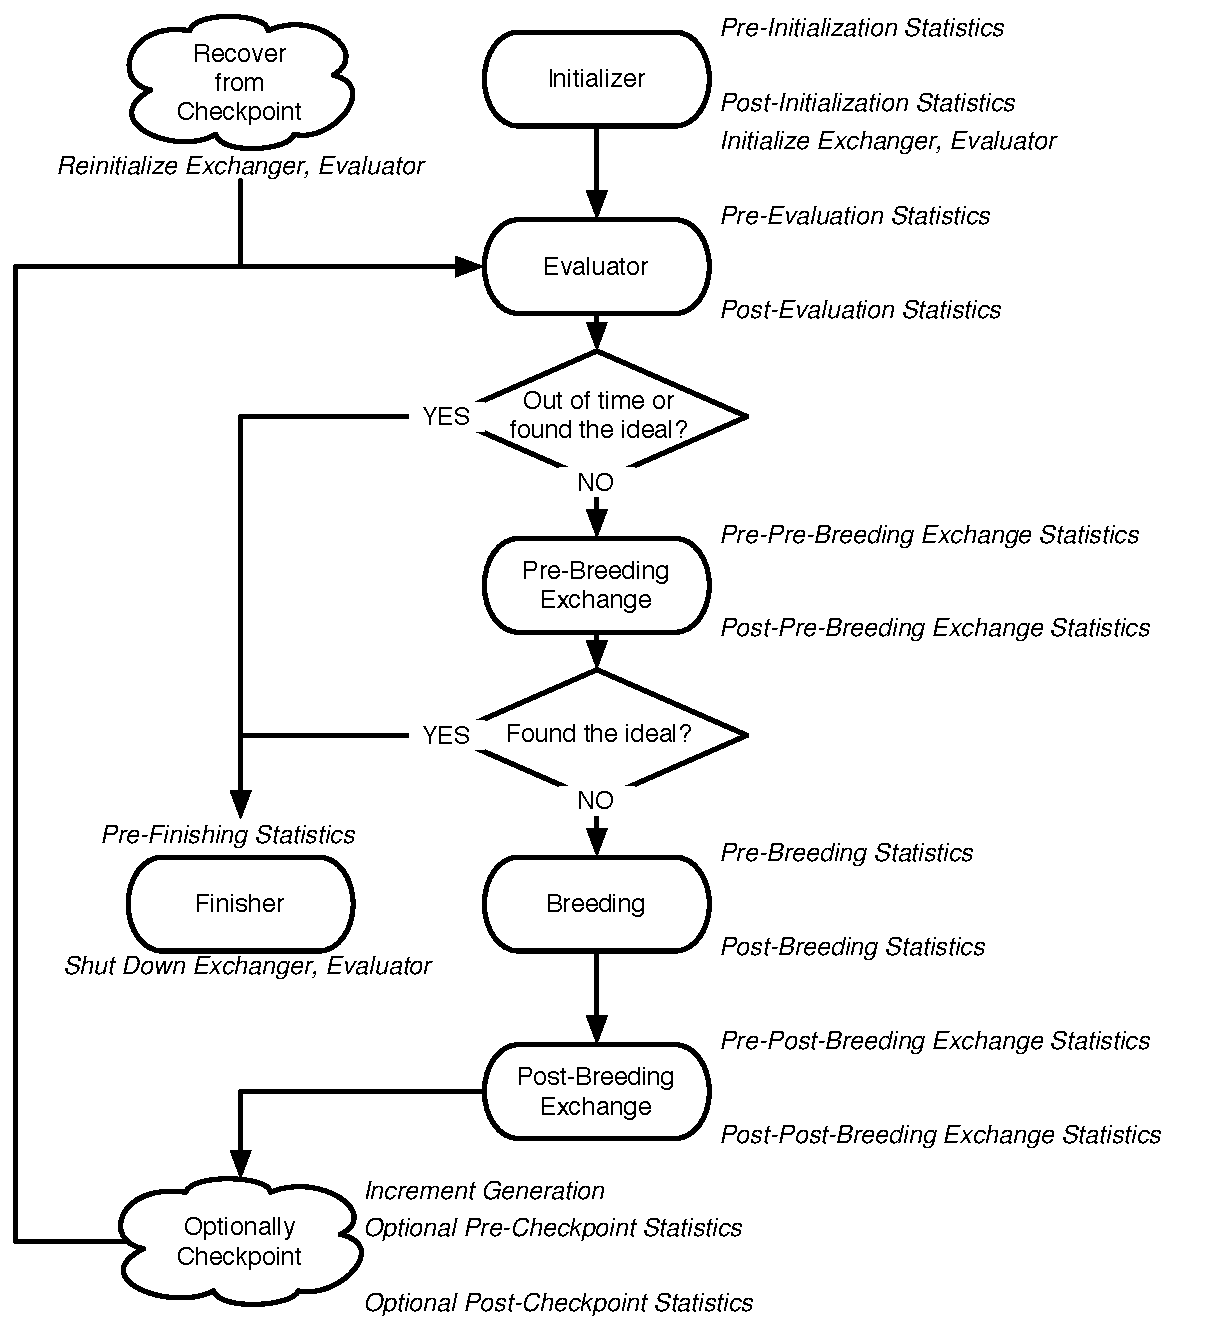
\includegraphics[height=6.3in]{EvolutionState.pdf}
\end{center}
\caption{Top-Level Loop of ECJ's \class{SimpleEvolutionState} class, used for basic generational EC algorithms.  Various sub-operations are shown occurring before or after the primary operations.  The full population is revised each iteration. }
\label{EvolutionState}
\end{figure}
\afterpage{\clearpage}

\section{Overview}

ECJ is a general-purpose evolutionary computation framework which attempts to permit as many valid combinations as possible of individual representation and breeding method, fitness and selection procedure, evolutionary algorithm, and parallelism.

\paragraph{Top-level Loop}  ECJ hangs the entire state of the evolutionary run off of a single instance of a subclass of \class{EvolutionState}.  This enables ECJ to serialize out the entire state of the system to a checkpoint file and to recover it from the same.  The \class{EvolutionState} subclass chosen defines the kind of top-level evolutionary loop used in the ECJ process.  We provide two such loops: a simple generational loop with optional elitism, and a steady-state loop.


\begin{figure}[t]
\begin{center}
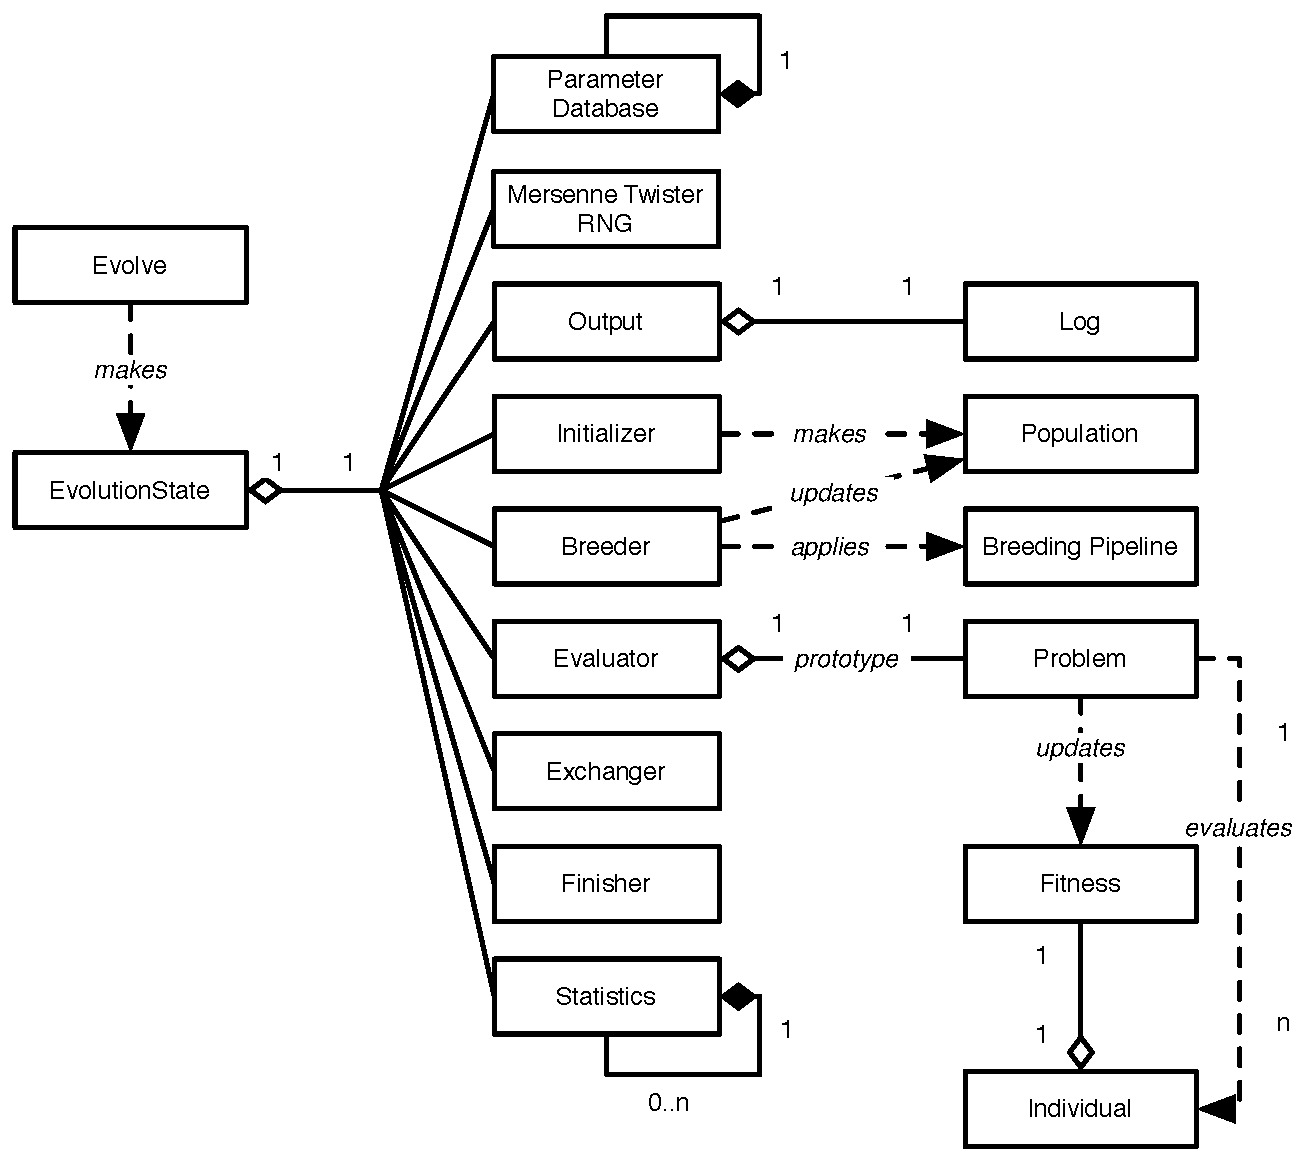
\includegraphics[width=5in]{Operators.pdf}
\end{center}
\caption{Top-Level operators and utility facilities in EvolutionState, and their relationship to certain state objects.}
\label{Operators}
\end{figure}

Figure \ref{EvolutionState} shows the top-level loop of the simple generational \class{EvolutionState}.  The loop iterates between breeding and evaluation, with an optional ``exchange'' period after each.  \class{Statistics} hooks are called before and after each period of breeding, evaluation, and exchanging, as well as before and after initialization of the population and ``finishing'' (cleaning up prior to quitting the program).

Breeding and evaluation are handled by singleton objects known as the \class{Breeder} and \class{Evaluator} respectively.  Likewise, population initialization is handled by an \class{Initializer} singleton, and finishing is done by a \class{Finisher}.  Exchanges after breeding and after evaluation are handled by an \class{Exchanger}.  The particular versions of these singleton objects are determined by the experimenter, though we provide versions which perform common tasks.  For example, we provide a traditional-EA \class{SimpleEvaluator}, a steady-state EA \class{SteadyStateEvaluator}, a ``single-population coevolution'' \class{CompetitiveEvaluator}, and a multi-population coevolution \class{MultiPopCoevolutionaryEvaluator}, among others.  There are likewise custom breeders and initializers for different functions.  The \class{Exchanger} provides an opportunity for other hooks, notably internal and external island models.  For example, post-breeding exchange might allow external immigrants to enter the population, while emmigrants might leave the population during post-evaluation exchange.  These singleton operators comprise most of the high-level ``verbs'' in the ECJ system, as shown in Figure \ref{Operators}.

\paragraph{Parameterized Construction}  ECJ is unusually heavily parameterized: practically every feature of the system is determined at runtime from a parameter.  Parameters define the classes of objects, the specific subobjects they hold, and all of their initial runtime values.  ECJ does this through a bootstrap class called \class{Evolve}, which loads a \class{ParameterDatabase} from runtime parameter files at startup.  Using this database, \class{Evolve} constructs the top-level \class{EvolutionState} and tells it to ``setup'' itself.  \class{EvolutionState} in turn calls subsidiary classes (such as \class{Evaluator}) and tells them to ``setup'' themselves from the database.  This procedure continues down the chain until the entire system is constructed.

\paragraph{State Objects}  In addition to ``verbs'', \class{EvolutionState} also holds ``nouns'' --- the state objects representing the things being evolved.  Specifically, \class{EvolutionState} holds exactly one \class{Population}, which contains some \(N\) (typically 1) \class{Subpopulation}s.  Multiple \class{Subpopulation}s permit experiments in coevolution, internal island models, etc.  Each \class{Subpopulation} holds some number of \class{Individual}s and the \class{Species} to which the \class{Individual}s belong.  \class{Species} is a flyweight object for \class{Individual}: it provides a central repository for things common to many \class{Individuals} so they don't have to each contain them in their own instances.

\begin{figure}
\begin{center}
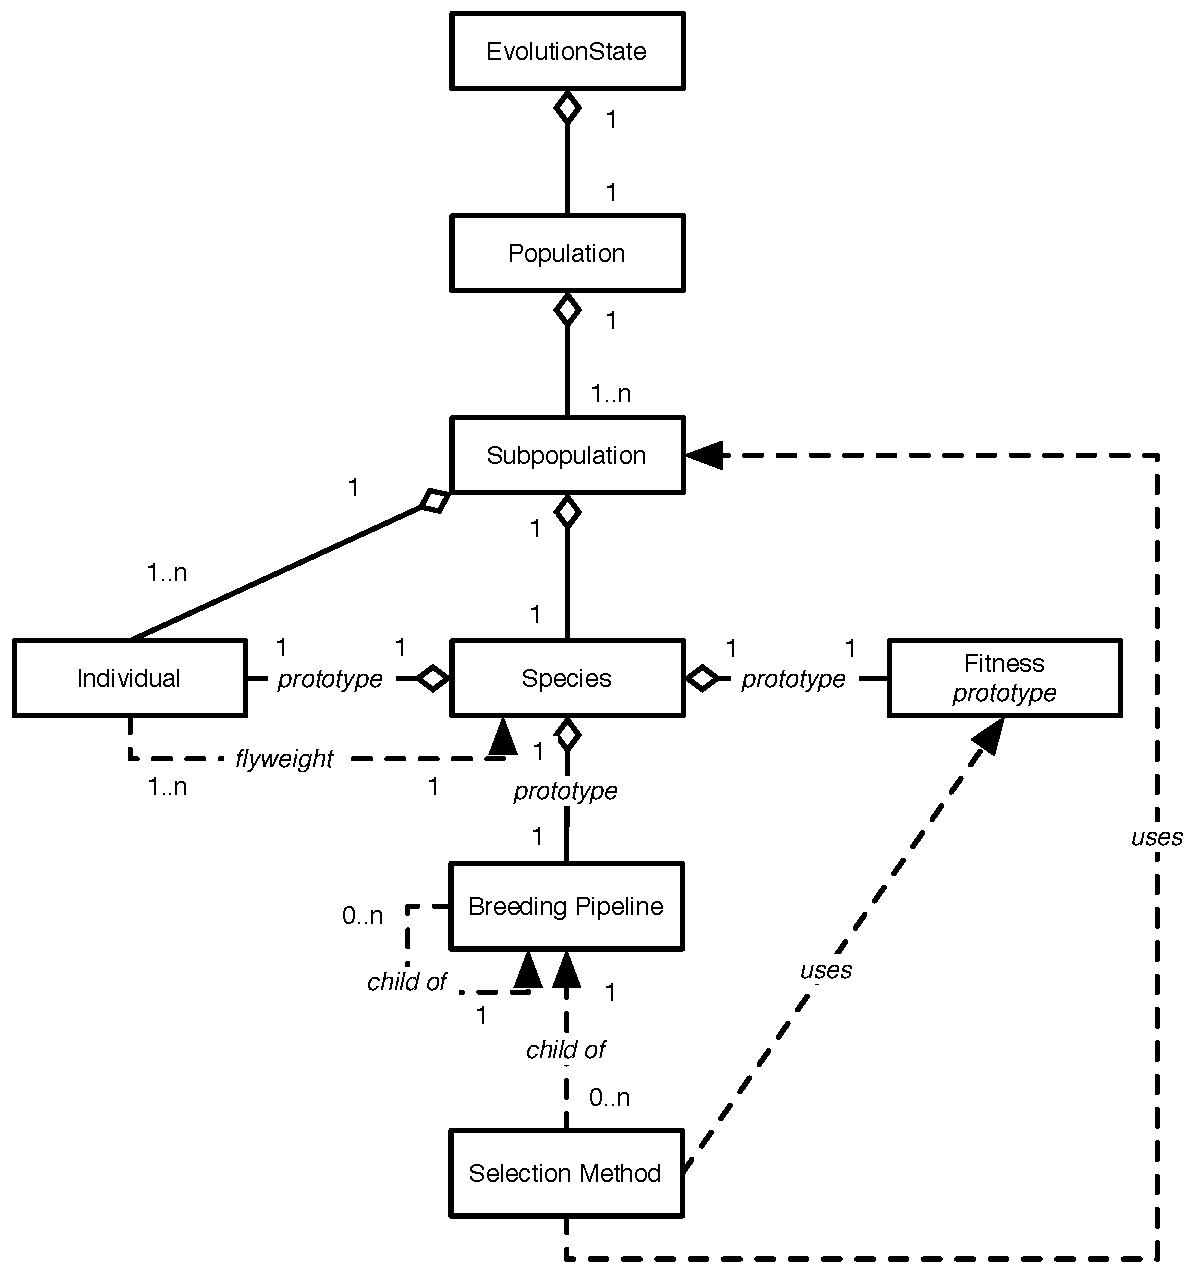
\includegraphics[width=4.7in]{StateObjects.pdf}
\end{center}
\caption{Top-Level data objects used in evolution.}
\label{StateObjects}
\end{figure}

While running, numerous state objects must be created, destroyed, and recreated.  As ECJ only learns the specific classes of these objects from the user-defined parameter file at runtime, it cannot simply construct them using Java's \class{new} operator.  Instead such objects are created by constructing a {\it prototype} object at startup time, and then using this object to stamp out copies of itself as often as necessary.  For example, \class{Species} contains a prototypical \class{Individual}.  When new \class{Individuals} must be created for a given \class{Subpopulation}, they are copied from the \class{Subpopulation}'s \class{Species} and then customized.  This allows different \class{Subpopulation}s to use different \class{Individual} representations.

In keeping with its philosophy of orthogonality, ECJ defines \class{Fitness}es separate from \class{Individual}s (representations), and provides both single-objective and multi-objective \class{Fitness} subclasses.  For historical reasons, \class{Subpopulation} stores the \class{Fitness} prototype, rather than keeping it in \class{Species}.  Different \class{Subpopulation}s may likewise use different \class{Fitness} forms.

\paragraph{Breeding} 

A \class{Species} holds a prototypical {\it breeding pipeline} which is cloned by the \class{Breeder} and used per-thread to breed individuals and form the next-generation population.  Breeding pipelines are tree structures where a node in the tree filters incoming \class{Individual}s from its child nodes and hands them to its parents.  The leaf nodes in the tree are \class{SelectionMethod}s which simply choose \class{Individual}s from the old subpopulation and hand them off.  There exist \class{SelectionMethod}s which perform tournament selection, fitness proportional selection, truncation selection, etc.  Nonleaf nodes in the tree are \class{BreedingPipeline}s, many of which copy and modify their received \class{Individual}s before handing them to their parent nodes.  Some \class{BreedingPipeline}s are representation-independent: for example, \class{MultiBreedingPipeline} asks for \class{Individual}s from one of its children at random according to some probability distribution.  But most \class{BreedingPipeline}s act to mutate or cross over \class{Individual}s in a representation-dependent way.  For example, the GP \class{CrossoverPipeline} asks for one \class{Individual} of each of its two children, which must be genetic programming \class{Individual}s, performs subtree crossover on those \class{Individual}s, then hands them to its parent.

A tree-structured breeding pipeline allows for a rich assortment of experimenter-defined selection and breeding proceses.  Further, ECJ's pipeline is {\it copy-forward}: \class{BreedingPipeline}s must ensure that they copy \class{Individual}s before modifying them or handing them forward, if they have not been already copied.  This guarantees that new \class{Individual}s are copies of old ones in the population, and furthermore that multiple pipelines may operate on the same \class{Subpopulation} in different threads without the need for locking.  ECJ may apply multiple threads to parallelize the breeding process without the use of Java synchronization at all.

\paragraph{Evaluation}

The \class{Evaluator} performs evaluation of a population by passing one or (for coevolutionary evaluation) several \class{Individual}s to a \class{Problem} subclass which the \class{Evaluator} has cloned off of its prototype.  Evaluation may too be done in multithreaded fashion with no locking, using one \class{Problem} per thread.  \class{Individual}s may also undergo repeated evaluation in coevolutionary \class{Evaluator}s of different sorts.

In most projects using ECJ, the primary task is to construct an appropriate \class{Problem} subclass.  The task of the \class{Problem} is to assess the fitness of the \class{Individual}(s) and set its \class{Fitness} accordingly.  \class{Problem} classes also report if the ideal \class{Individual} has been discovered.

\paragraph{Utilities}

In addition to its \class{ParameterDatabase}, ECJ also uses a checkpointable \class{Output} convenience facility which maintains various streams, repairing them after checkpoint.  \class{Output} also provides for message logging, retaining in memory all messages during the run, so that on checkpoint recovery the messages are printed out again as before.  Other utilities include population distribution selectors, searching and sorting tools, etc.

The quality of a random number generator is important for a stochastic optimization system.  As such, ECJ's random number generator was the very first class written in the system: it is a Java implementation of the highly respected Mersenne Twister algorithm \cite{mersennetwister} and is the fastest such implementation available.  Since ECJ's release, the ECJ \class{MersenneTwister} and \class{MersenneTwisterFast} classes have found their way in a number of unrelated public-domain systems, including the popular NetLogo multiagent simulator \cite{Tisue04netlogo:a}.  \class{MersenneTwisterFast} is also shared in ECJ's sister software, the MASON multiagent simulation toolkit \cite{luke.cioffi-revilla.ea:mason}.

\paragraph{Representations and Genetic Programming}

ECJ allows you to specify any genome representation you like.  Standard representation packages in ECJ provide functionality for vectors of all Java data types; arbitrary-length lists; trees; and collections of objects (such as rulesets).



\begin{figure}[t]
\begin{center}
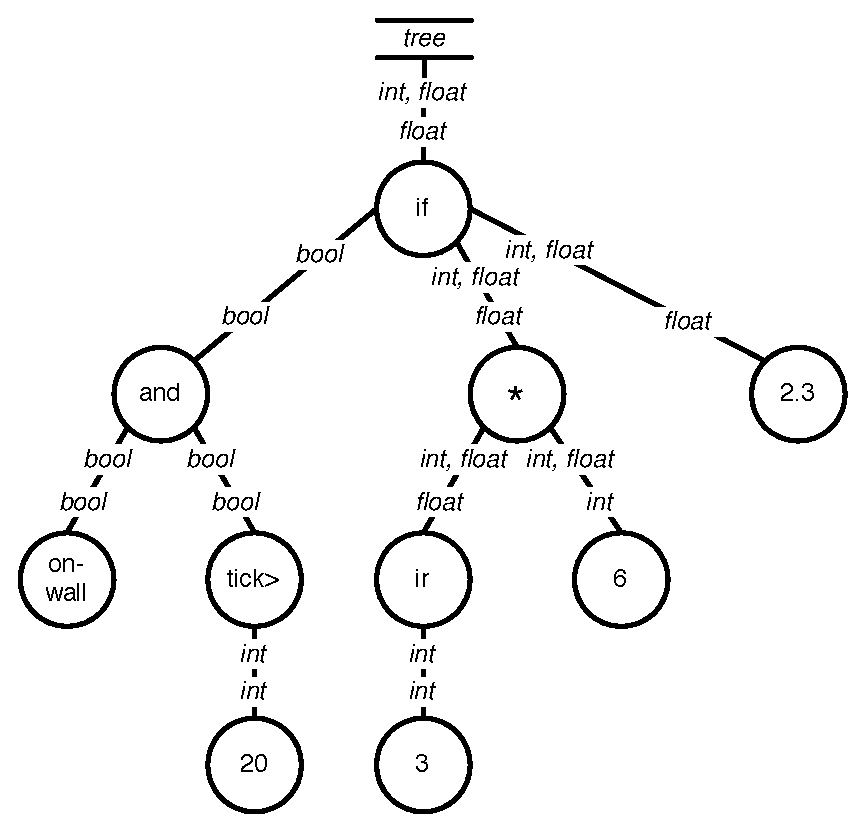
\includegraphics[width=4in]{parsetree.pdf}
\end{center}
\caption{A typed genetic programming parse tree.}
\label{parsetree}
\end{figure}


ECJ is perhaps best known for its support of ``Koza''-style tree-structured genetic programming representations.  ECJ represents these individuals as forests of parse-trees, each tree equivalent to a single Lisp s-expression.  Figure \ref{parsetree} shows a parse-tree for a simple robot program, equivalent to the Lisp s-expression \mbox{\class{(if (and on-wall (tick\(>\) 20) (\(\ast\) (ir 3) 6) 2.3).}}  In C this might look like \mbox{\class{ (onWall \&\& tick \(>\) 20) ? ir(3) * 6 : 2.3}.}  This notionally says ``If I'm on the wall and my tick-count is greater than 20, then return the value of my third infrared sensor times six, else return 2.3''.  Such parse-trees are typically evaluated by executing their programs in a test environment, and modified via subtree crossover (swapping subtrees among individuals) or various kinds of mutation (replacing a subtree with a randomly-generated one, perhaps).  

ECJ allows multiple subtrees for various experimental needs: Automatically Defined Functions (ADFs\,---\,a mechanism for evolving subroutine calls \cite{koza:gp2}), or parallel program execution, or evolving teams of programs.  Along with ADFs, ECJ provides built-in support for Automatically Defined Macros (ADMs) \cite{adm} and Ephemeral Random Constants (ERCs \cite{koza:book}, such as the numbers 20, 3, 6, and 2.3 in Figure \ref{parsetree}).

Genetic programming trees are constructed out of a ``primorial soup'' of function templates (such as \class{on-wall} or \class{2.3}.  Early forms of genetic programming were typeless: though such templates had a predefined arity (number of arguments), any node could be connected to any other.  Many genetic programming needs require more constraints than this.  For example, the node \class{if} might expect a boolean value in its first argument, and integers or floats in the second and third arguments, and return a float when evaluated.  Similarly \class{and} might take two booleans as arguments and return a boolean, while \class{\(\ast\)} would take ints or floats as arguments and return a float.

Such types are often associated with the kinds of data passed from node to node, but they do not have to be.  For example, typing might be used to constrain certain nodes to be evaluated in groups or in a certain order: for example, a function \class{type-block} might insist that its first argument be of type \textit{foo} and its second argument be of type \textit{bar} to make certain that a \textit{foo} node be executed before a \textit{bar} node.

ECJ permits a simple static typing mechanism called {\it set-based} typing, which is suitable for many such tasks.  In set-based typing, the return type and argument types of each node are each defined to be  sets of type symbols (for example, \{\textit{bool}\} or \{\textit{foo, bar, baz}\}, or \{\textit{int, float}\}.  The desired return type for the tree's root is similarly defined.  A child node is permitted to fit into the argument slot of a parent node if the child node's return type and type of the that argument slot in the parent are {\it compatible}.  We define types to be compatible if their set intersection is nonempty (that is, they share at least one type symbol).

Set-based typing is sufficient for the typing requirements found in many programming languages, including ones with type hierarchies.  It allows, among other things, for nodes such as \class{\(\ast\)} to accept {\it either} integers or floats.  However there are considerable restrictions on the power of set-based typing.  It's often useful for the return type of a node to {\it change} based on the particular nodes which have plugged into it as arguments. For example, \class{\(\ast\)} might be defined as returning a float if at least one of its arguments returns floats, but returning an integer if both of its arguments return integers.  \class{if} might be similarly defined not to return a particular type, but to simply require that its return type and the second and third argument types must all match.  Such ``polymorphic'' typing is particularly useful in situations such as matrix multiplication, where the operator must place constraints on the width and height of its arguments and the final returned matrix.  In this example, it's also useful to have an infinite number of types (perhaps to represent matrices of varying widths or heights).

ECJ does not support polymorphic typing out of the box simply because it is difficult to implement many if not most common tree modification and generation algorithms using polymorphic typing: instead, set-based typing is offered to handle as many common needs as can be easily done. 

\paragraph{Out of the Box Capabilities}

ECJ provides support out-of-the-box for a bunch of algorithm options:

\begin{itemize}
\item Generational algorithms: \((\mu,\lambda)\) and \((\mu+\lambda)\) Evolution Strategies, the Genetic Algorithm, Genetic Programming variants, and Differential Evolution
\item Steady-State evolution
%\item Particle Swarm Optimization
\item Parsimony pressure algorithms
\item Spatially-embeded evolutionary algorithms
\item Random restarts
\item Multiobjective optimization, including the NSGA-II and SPEA2 algorithms.
\item Cooperative, 1-Population Competitive, and 2-Population Competitive coevolution.
\item Multithreaded evaluation and breeding.
\item Parallel synchronous and asynchronous Island Models spread over a grid of computers.
\item Internal synchronous Island Models internally in a single ECJ process.
\item Massive parallel generational fitness evaluation of individuals on remote slave machines.
\item Asynchronous Evolution, a version of steady-state evolution with massive parallel fitness evaluation on remote slave machines.
\item Opportunistic Evolution, where remote slave machines run their own mini-evolutionary processes for a while before sending individuals back to the master process.
\item Internal synchronous Island Models internally in a single ECJ process.
\item A large number of selection and breeding operators
\end{itemize}

ECJ also has a GUI, though in truth I nearly universally use the command-line.

\paragraph{Idiosyncracies}

ECJ was developed near the introduction of Java and so has a lot of historical idiosyncracies.\footnote{It used to have a lot more\,---\,I've been weeding out ones that I think are unnecessary nowadays!}.  Some of them exist to this day because of conservatism: refactoring is disruptive.  If you code with ECJ, you'll definitely have to get used to one or more of the following:

\begin{itemize}
\item No generics at all, few iterators or enumerators, no Java features beyond 1.4 (including annotations), and little use of the Java Collections library.  This is part historical, and part my own dislike of Java's byzantine generics implementation, but it's mostly efficiency.  Generics are very slow when used with basic data types, as they require boxing and unboxing.  The Java Collections library is unusually badly written in many places internally: and anyway, for speed we tend to work directly with arrays.  

\item Hand-rolled socket code.  ECJ's parallel facility doesn't rely on other libraries.

\item ECJ loads nearly every object from its parameter database.  This means that you'll rarely see the \variable{new} keyword in ECJ, nor any constructors.  Instead ECJ's usual ``constructor'' method is a method called \method{setup(...)}, which sets up an object from the database.

\item A proprietary logging facility.  ECJ was developed before the existence of \class{java.util.logging}.  Partly out of conservatism, I am hesitant to rip up all the pervasive logging just to use Sun's implementation (which isn't very good anyway).

\item A parameter database derived from Java's old \class{java.util.Properties} list rather than XML.  This is historical of course.  But seriously, do I need a justification to avoid XML?  

\item Mersenne Twister random number generator. \class{java.lang.Random} is grotesquely bad, and systems which use it should be shunned.

\item A Makefile.  ECJ was developed before Ant and I've personally never needed it.

\end{itemize}

\section{Unpacking ECJ and Using the Tutorials}

ECJ comes as a single tarball, \file{ecj.tar.gz}, or as a ZIP file, \file{ecj.zip}.  After unpacking this, you're left with one directory called \file{ec}.

In the \file{ec} directory you'll find several items:

\begin{itemize}
\item A top-level \file{README} file, which should be self-explanatory in its importance.
\item ECJ's \file{LICENSE} file, which describes the primary license (AFL 3.0, a BSD-style academic license).
\item A \file{CHANGES} log, which lists all past changes to all versions (including the latest).
\item A \file{Makefile}.  ECJ does not use Ant, and in fact you can compile ECJ very straightforwardly by simply compiling all the java files in the \file{ec} directory.  But we provide a helpful Makefile which will compile ECJ and do various other useful tasks.
\item The \file{docs} directory.  This contains most of the ECJ documentation.
\item The \file{start} directory.  This contains various scripts for starting up ECJ: though in truth we rarely use them.
\item The \file{ec} directory.  This contains ECJ proper.  \file{ec} is the top-level package for ECJ.
\end{itemize}

\subsection{The \file{ec} Directory, the CLASSPATH, and jar files}

The \file{ec} directory is ECJ's top-level package.  Every subdirectory is a subpackage, and most of them are headed by helpful README files which describe the contents of the directory.  Most packages contain not only Java files and class files but also parameter files and occasional data files: ECJ was designed originally for the class files to be compiled and stored right alongside the Java files in these directories, though it can be used with the separate-build-area approach taken by IDEs like Eclipse.

Because \file{ec} is the top-level package, you can compile ECJ, more or less, by just sticking its parent directory (the \file{ecj} directory), in your CLASSPATH.  You will also need to add certain {\bf jar files} in order to compile ECJ's distributed evaluation and island model facilities, and its GUI.  You can get these jar files from the ECJ main website (http://cs.gmu.edu/\(\sim\)eclab/projects/ecj/).  Note that none of these libraries is required.  For example, if the libraries for the distributed evaluator and island model are missing, ECJ will compile but will complain if you try to run those packages with compression turned on (a feature of the packages).  The GUI library is optional to ECJ, so if you don't install its libraries, you can still compile ECJ by just deleting the \file{ec/display} directory.

\subsubsection{The \file{ec/display} Directory: ECJ's GUI}

This directory contains ECJ's GUI.  It's in a state of disrepair and I suggest you do not use it.  ECJ is really best as a command line program.  In fact, as mentioned above, you can simply delete the directory and ECJ will compile just fine.

\subsubsection{The \file{ec/app} Directory: Demo Applications}

This directory contains all the demo applications.  We have quite a number of demo applications, many sharing the same subdirectories.  Read the provided README file for some guidance.

\subsection{The \file{docs} Directory}

This directory contains all top-level documentation of ECJ except for the various README files scattered throughout the package.  The \file{index.html} file provides the top-level entry point to the documentation.

The documentation includes:

\begin{itemize}
\item Introduction to parameters in ECJ
\item Class documentation
\item ECJ's four tutorials and post-tutorial discussion.  The actual tutorial code is located in the \file{ec/app} directory.
\item An (old) overview of ECJ
\item An (old) discussion of ECJ's warts
\item Some (old) graph diagrams of ECJ's structure
\item This manual
\end{itemize}

\subsubsection{Tutorials}

ECJ has four tutorials which introduce you to the basics of coding on the system.  {\bf I strongly suggest you go through them before continuing through the rest of this manual.}  They are roughly:

\begin{enumerate}
\item A simple GA to solve the MaxOnes problem with a boolean representation.
\item A GA to solve an integer problem, with a custom mutation pipeline.
\item An evolution strategy to solve a floating-point problem, with a custom statistics object and reading and writing populations.
\item A genetic programming problem, plus some elitism.
\end{enumerate}

As should be obvious from the rest of this manual, this {\bf barely scratches the surface} of ECJ.  No mention is given of parallelism, differential evolution, coevolution, multiobjective optimization, list and ruleset representations, grammatical encoding, spatial embedding, etc.  But it'll get you up to speed.

\chapter{\class{ec.Evolve} and Utility Classes}
\label{ec.Evolve}

ECJ is big.  Let us begin.
\vspace{4em}

\noindent ECJ's entry point is the class \class{ec.Evolve}.  This class is little more than bootstrapping code to set up the ECJ system, construct basic datatypes, and get things going.

To run an ECJ process, you fire up \class{ec.Evolve} with certain runtime arguments.

\script{%
java ec.Evolve -file \textit{myParameterFile.params} -p \textit{param=value} -p \textit{param=value}\hfill{\it (etc.)}
}

ECJ sets itself up entirely using a {\bf parameter file}.  To this you can add additional {\bf command-line parameters} which override those found in the parameter file.  More on the parameter file will be discussed starting in Section~\ref{parameterdatabase}.

ECJ can also restart from a checkpoint file it created in a previous run, like this:

\script{%
java ec.Evolve -checkpoint \textit{myCheckpointFile.gz}
}

Checkpointing will be discussed in Section~\ref{checkpointing}.

The purpose of \class{ec.Evolve} is to construct an \class{ec.EvolutionState} instance, or load one from a checkpoint file; then get it running; and finally clean up.  The \class{ec.EvolutionState} class actually performs the evolutionary process.   Most of the stuff \class{ec.EvolutionState} holds is associated with evolutionary algorithms or other stochastic optimization procedures.  However there are certain important utility objects or data which are created by \class{ec.Evolve} prior to creating the \class{ec.EvolutionState}, and are then stored into \class{ec.EvolutionState} after it has been constructed.  These objects are:

\begin{itemize}
\item The {\bf Parameter Database}, which holds all the parameters \class{ec.EvolutionState} uses to build and run the process.
\item The {\bf Output}, which handles logging and writing to files.
\item The {\bf Checkpointing Facility} to create checkpoint files as the process continues.
\item The {\bf Number of Threads} to use, and the {\bf Random Number Generators}, one per thread.
\item A simple declaration of the {\bf Number of Jobs} to run in the process.
\end{itemize}

The remainder Section~\ref{ec.Evolve} discusses each of these items.  It's not the most exciting of topics: but it's important in order to understand the rest of the ECJ process.

\section{The Parameter Database}
\label{parameterdatabase}

To build and run an experiment in ECJ, you typically write three things:

\begin{itemize}
\item (In Java) A {\bf problem} which evaluates individuals and assigns fitness values to them.
\item (In Java) Depending on the kind of experiment, various {\bf components} from which individuals can be constructed\,---\,for example, for a genetic programming experiment, you'll need to define the kinds of nodes which can be used to make up the individual's tree.
\item (In one or more Parameter Files) Various {\bf parameters} which define the kind of algorithm you are using, the nature of the experiment, and the makeup of your populations and processes.
\end{itemize}

Let's begin with the third item.  Parameters are the lifeblood of ECJ: practically everything in the system is defined by them.  This makes ECJ highly flexible; but it also adds complexity to the system.

ECJ loads parameter files and stores them into the \class{ec.util.ParameterDatabase} object, which is available to nearly everything.  Parameter files are an extension of the files used by Java's old {\bf java.util.PropertyList} object.  Parameter files usually end in \textstr{.params}, and contain parameters one to a line.  Parameter files may also contain blank (all whitespace) lines, which are ignored, and also lines which start with \character{\#}, which are considered comments and also ignored.  An example comment:
\begin{quote}
\texttt{\# This is a comment}
\end{quote}

The parameter lines in a parameter file typically look like this:
\begin{quote}
{\it parameter.name} = {\it parameter value}
\end{quote}

A {\bf parameter name} is a string of non-whitespace characters except for \character{=}.  After this comes some optional whitespace, then an \character{=}, then some more optional whitespace.\footnote{Actually, you can omit the \character{=}, but it's considered bad style.}  A {\bf parameter value} is a string of characters, including whitespace, except that all whitespace is trimmed from the front and end of the string.  Notice the use of a period the parameter name.  It's quite a common convention to use periods in various parameter names in ECJ. We'll get to why in a second.

Here are some legal parameter lines:

\params{%
generations = 400\\
pop.subpop.0.size\hspace{1in}=1000\\
pop.subpop=\hspace{2in}ec.Subpopulation\\
}

Here are some illegal parameter lines:

\params{%
generations\\
= 1000\\
pop subpop = ec.Subpopulation
}

\subsection{Inheritance}
Parameter files may be set up to {\bf derive from} one or more other parameter files.  Let's say you have two parameter files, \file{a.params} and \file{b.params}.  Both are located in the same directory.  You can set up \file{a.params} to derive from \file{b.params} by adding the following line as the very first line in the \file{a.params} file:


\params{%
parent.0 = b.params
}

This says, in effect: ``include in me all the parameters found in the \file{b.params} file, but any parameters I myself declare will override any parameters of the same name in the \file{b.params} file.''  Note that \file{b.params} may itself derive from some other file (say, \file{c.params}).  In this case, \file{a.params} receives parameters from both (and parameters in \file{b.params} will likewise override ones of the same name in \file{c.params}).

Let's say that \file{b.params} is located inside a subdirectory called \file{foo}.  Then the line will look like this:

\params{%
parent.0 = foo/b.params
}

Notice the forward slash: ECJ was designed on UNIX systems.  Likewise, imagine if \file{b.params} was stored in a sibling directory called \file{bar}: then we might say:

\params{%
parent.0 = ../bar/b.params
}

Long story short: parameter files are declared using traditional UNIX path syntax.

A parameter file can also derive from {\it multiple} parent parameter files, by including each at the beginning of the file, with consecutive numbers, like this:


\params{%
parent.0 = b.params\\
parent.1 = yo/d.params\\
parent.2 = ../z.params
}

This says in effect: ``first look in \file{a.params} for the parameter.  If you can't find it there, look in \file{b.params} and, ultimately, all the files \file{b.params} derives from.  If you can't find it in any of them, look in \file{d.params} and all the files it derives from.  If you can't find it in any of them, look in \file{z.params} and all the files it derives from.  If you've still not found the parameter, give up.''

This is essentially a depth-first search through a tree or DAG, with parents overriding their children (the files they derive from) and earlier siblings overriding later siblings.  Note that this multiple inheritance scheme is not the same as C++ or Lisp/CLOS, which use a distance measure! 

When you fire up ECJ, you point it at a single parameter file, and you can provide additional parameters at the command-line, like this:

\script{%
java ec.Evolve -file \textit{parameterFile.params} -p \textit{command-line-parameter=value} \textbackslash \\
\hsp{21.15em}-p \textit{command-line-parameter=value} ...
}

Furthermore, your program itself can submit parameters to the parameter database, though it's very unusual to do so.  When a parameter is requested from the parameter database, here's how it's looked up:

\begin{enumerate}
\item If the parameter was declared by the program itself, this value is returned.
\item Else if the parameter was provided on the command line, this value is returned.
\item Else the parameter is looked up in the provided parameter file and all derived files using the inheritance ordering described earlier.
\item Else the database signals failure.
\end{enumerate}


\subsection{Kinds of Parameters}
\label{kindsofparameters}

ECJ supports the following kinds of parameters:

\begin{itemize}
\item {\bf Numbers}.  Either long integers or double floating-point values.  Examples:

\params{%
generations = 500\\
tournament.size = 3.25\\
minimum-fitness = -23.45e15\\
}

\item {\bf Arbitrary Strings} trimmed of whitespace.  Example:

\params{%
crossover-type = two-point\\
}

\item {\bf Booleans}.  Any value except for \textstr{false} (case-insensitive) is considered to be {\it true}.  It's best style to use lower-case  \textstr{true}  and  \textstr{false}.  The first two of these examples are {\it false} and the second two are {\it true}:

\params{%
print-params = false\\
%verbose = false\\
die-silently = fAlSe\\
pop.subpop.0.perform-injections = true\\
quit-on-run-complete = whatever\\
}

\item {\bf File Path Names}.  Paths can be of three types.  {\bf Absolute paths}, which (in UNIX) begin with a \character{/}, stipulate a precise location in the file system.  {\bf Relative paths}, which do not begin with a \character{/}, are defined relative to the parameter file in which the parameter was located.  You've seen relative paths already used for derived parameter files.  Finally, {\bf Execution relative paths} are defined relative to the directory in which the ECJ process was launched.  Execution relative paths look exactly like relative paths except that they begin with the special character \character{\$}.  Examples of all three kinds of paths:


\params{%
stat.file = \$out.stat\\
eval.prob.map-file = ../dungeon.map\\
temporary-output-file = /tmp/output.txt
}

\item {\bf Class Names}.   Class names are defined as the full class name of the class, including the package.  Example:


\params{%
pop.subpop.0.species = ec.gp.GPSpecies
}

\item {\bf Arrays}.   ECJ doesn't have direct support for loading arrays, but has a convention you should be made aware of.  It's common for arrays to be loaded by first stipulating the number of elements in the array, then stipulating each array element in turn, starting with 0.  The parameter used for the number of elements differs from case to case.  Note the use of periods prior to each number in the following example:


\params{%
gp.fs.0.size = 6\\
gp.fs.0.func.0 = ec.app.ant.func.Left\\
gp.fs.0.func.1 = ec.app.ant.func.Right\\
gp.fs.0.func.2 = ec.app.ant.func.Move\\
gp.fs.0.func.3 = ec.app.ant.func.IfFoodAhead\\
gp.fs.0.func.4 = ec.app.ant.func.Progn2\\
gp.fs.0.func.5 = ec.app.ant.func.Progn3
}

The particulars vary.  Here's another, slightly different, example:


\params{%
exch.num-islands = 8\\
exch.island.0.id = SurvivorIsland\\
exch.island.1.id = GilligansIsland\\
exch.island.2.id = FantasyIsland\\
exch.island.3.id = TemptationIsland\\
exch.island.4.id = RhodeIsland\\
exch.island.5.id = EllisIsland\\
exch.island.6.id = ConeyIsland\\
exch.island.7.id = TreasureIsland
}

Anyway, you get the idea.

\end{itemize}

\subsection{Namespace Hierarchies and Parameter Bases}

ECJ has lots of parameters, and by convention organizes them in a namespace hierarchy to maintain some sense of order.    The delimiter for paths in this hierarchy is\,---\, you guessed it\,---\,the period. 

The vast majority of parameters are used by one Java object or another to set itself up immediately after it has been instantiated for the first time.  ECJ has an important convention which uses the namespace hierarchy to do just this: the {\bf parameter base}.  A parameter base is essentially a path (or namespace, what have you) in which an object expects to find all of its parameters.  The prefix for this path is typically the parameter name by which the object itself was loaded.

For example, let us consider the process of defining the class to be used for the global population.  This class is found in the following parameter:

\params{%
pop = ec.Population
}

ECJ looks for this parameter, expects a class (in this case, \class{ec.Population}), loads the class, and creates one instance.  It then calls a special method (\method{setup(...)}, we'll discuss it later) on this class so it can set itself up from various parameters.  In this case, \class{ec.Population} needs to know how many subpopulations it will have.  This is defined by the following parameter:

\params{%
pop.subpops = 2
}

\class{ec.Population} didn't know that it was supposed to look in \parameter{pop.subpops} for this value.  Instead, it only knew that it needed to look in a parameter called \parameter{subpops}.  The rest (in this case, \parameter{pop}) was provided to \class{ec.Population} as its {\it parameter base}: the text to be prepended\,---\,plus a period\,---\,to all parameters that \class{ec.Population} needed to set itself up.  It's not a coincidence that the parameter base also happened to be the very parameter which defined \class{ec.Population} in the first place.  This is by convention.

Armed with the fact that it needs to create an array of two subpopulations, \class{ec.Population} is ready to load the classes for those two subpopulations.  Let's say that for our experiment we want them to be of different classes.  Here they are:

\params{%
pop.subpop.0 = ec.Subpopulation\\
pop.subpop.1 = ec.app.myapp.MySpecialSubpopulation
}

The two classes are loaded and one instance is created of each of them.  Then \method{setup(...)} is called on each of them.  Each subpopulation looks for a parameter called \parameter{size} to tell it how may individuals will be in that subpopulation.  Since each of them is provided with a different parameter base, they can have different sizes:

\params{%
pop.subpop.0.size = 100\\
pop.subpop.1.size = 512
}

Likewise, each of these subpopulations needs a ``species''.  Presuming that the species are different classes, we might have:

\params{%
pop.subpop.0.species = ec.vector.VectorSpecies\\
pop.subpop.1.species = ec.gp.GPSpecies
}

These species objects themselves need to be set up, and when they do, their parameter bases will be \parameter{pop.subpop.0.species} and \parameter{pop.subpop.1.species} respectively.  And so on.

Now imagine that we have ten subpopulations, all of the same class (\class{ec.Subpopulation}), and {\it all but the first one} has the exact same size.  We'd wind up having to write silly stuff like this: 

\vbox{
\params{%
pop.subpop.0.size = 1000\\
pop.subpop.1.size = 500\\
pop.subpop.2.size = 500\\
pop.subpop.3.size = 500\\
pop.subpop.4.size = 500\\
pop.subpop.5.size = 500\\
pop.subpop.6.size = 500\\
pop.subpop.7.size = 500\\
pop.subpop.8.size = 500\\
pop.subpop.9.size = 500
}}

That's a lot of typing.  Though I am saddened to report that ECJ's parameter files {\it do} require a lot of typing, at least the parameter database facility offers an option to save our fingers somewhat in this case.  Specifically, when the \class{ec.Subpopulation} class sets itself up each time, it actually looks in not one but {\it two} path locations for the \parameter{size} parameter: first it tacks on its current base (as above), and if there's no parameter at that location, then it tries tacking on a {\bf default base} defined for its class.  In this case, the default base for \class{ec.Subpopulation} is the prefix \parameter{ec.subpop}.  Armed with this we could simply write:

\vbox{
\params{%
ec.subpop.size = 500\\
pop.subpop.0.size = 1000
}}

When ECJ looks for subpopulation 0's size, it'll find it as normal (1000).  But when it looks for subpopulation 1 (etc.), it won't find a size parameter in the normal location, so it'll look in the default location, use what it finds there (500).  Only if there's no parameter to be found in either location will ECJ signal an error.

It's important to note that if a class is loaded from a default parameter, this doesn't mean that the default parameter will become its parameter base: rather, the original expect location will continue to be the base.  For example, imagine if both of our Species objects were the same class, and we had defined them using the default base.  That is, instead of

\params{%
pop.subpop.0.species = ec.vector.VectorSpecies\\
pop.subpop.1.species = ec.vector.VectorSpecies
}

\noindent ...we simply said  

\params{%
ec.subpop.species = ec.vector.VectorSpecies
}

When the species for subpopulation 0 is loaded, its parameter base is not going to be \parameter{ec.subpop.species}.  Instead, it will still be \parameter{pop.subpop.0.species}.  Likewise, the parameter base for the species of subpopulation 1 will still be \parameter{pop.subpop.1.species}.

Keep in mind that all of this is {\it just a convention}.  You can use periods for whatever you like ultimately.  And there exist a few global parameters without any base at all.  For example, the number of generations is defined as 

\params{%
generations = 200
}

\noindent ...and the seed for the random number generator the fourth thread is

\params{%
seed.3 = 12303421
}

\noindent ...even though there is {\it no object set up} with the \parameter{seed} parameter, and hence no object has \parameter{seed} as its parameter base.  Random number generators are one of the few rare objects in ECJ which are not specified from the parameter file.

\subsection{Loading Parameters}

Parameters are looked up in the \class{ec.util.ParameterDatabase} class, and parameter names are specified using the \class{ec.Parameter} class.  The latter is little more than a cover for Java strings.  To create the parameter \parameter{pop.subpop.0.size}, we say:

\java{%
Parameter param = new Parameter("pop.subpop.0.size");
}

Of course, usually we don't want to just make a direct parameter, but rather want to construct one from a parameter base and the remainder.  Let's say our base (\parameter{pop.subpop.0}) is stored in the variable \variable{base}, and we want to look for \parameter{size}.  We do this as:

\java{%
Parameter param = base.push("size");
}

Here are some common \class{ec.util.ParameterDatabase} methods:

\begin{methods}{ec.util.ParameterDatabase}
\mthd{public boolean exists(Parameter \textit{parameter}, Parameter \textit{default})}
If either parameter exists in the database, return true.  Either parameter may be null.
\mthd{public String getString(Parameter \textit{parameter}, Parameter \textit{default})}
Look first in {\it parameter}, then failing that, in {\it default parameter}, and return the result as a String, else null if not found.  Either parameter may be null.
\mthd{public File getFile(Parameter \textit{parameter}, Parameter \textit{default})}
Look first in {\it parameter}, then failing that, in {\it default parameter}, and return the result as a File, else null if not found.  Either parameter may be null.
\mthd{public Object getInstanceForParameterEq(Parameter \textit{parameter}, Parameter \textit{default}, Class \textit{superclass})}
Look first in {\it parameter}, then failing that, in {\it default parameter}, to find a class.  The class must have {\it superclass} as a superclass, or can be the {\it superclass} itself.  Instantiate one instance of the class using the default (no-argument) constructor, and return the instance.  Throws an \class{ec.util.ParamClassLoadException} if no class is found.
\mthd{public Object getInstanceForParameter(Parameter \textit{parameter}, Parameter \textit{default}, Class \textit{superclass})}
Look first in {\it parameter}, then failing that, in {\it default parameter}, to find a class.  The class must have {\it superclass} as a superclass, but may not be {\it superclass} itself.  Instantiate one instance of the class using the default (no-argument) constructor, and return the instance.  Throws an \class{ec.util.ParamClassLoadException} if no class is found.
\mthd{public int getBoolean(Parameter \textit{parameter}, Parameter \textit{default}, double \textit{defaultValue})}
Look first in {\it parameter}, then failing that, in {\it default parameter}, and return the result as a boolean, else \textit{defaultValue} if not found or not a boolean.  Either parameter may be null.

\mthd{public int getIntWithDefault(Parameter \textit{parameter}, Parameter \textit{default}, int \textit{defaultValue})}
Look first in {\it parameter}, then failing that, in {\it default parameter}, and return the result as an int, else \textit{defaultValue} if not found or not an int.  Either parameter may be null.
\mthd{public int getInt(Parameter \textit{parameter}, Parameter \textit{default}, int \textit{minValue})}
Look first in {\it parameter}, then failing that, in {\it default parameter}, and return the result as an int, else {\it minValue\(-1\)} if not found, not an int, or \(<\) minValue.  Either parameter may be null.
\mthd{public int getIntWithMax(Parameter \textit{parameter}, Parameter \textit{default}, int \textit{minValue}, int \textit{maxValue})}
Look first in {\it parameter}, then failing that, in {\it default parameter}, and return the result as an int, else {\it minValue\(-1\)} if not found, not an int, \(<\) minValue, or \(>\) maxValue.  Either parameter may be null.


\mthd{public long getLongWithDefault(Parameter \textit{parameter}, Parameter \textit{default}, long \textit{defaultValue})}
Look first in {\it parameter}, then failing that, in {\it default parameter}, and return the result as a long, else \textit{defaultValue} if not found or not a long.  Either parameter may be null.
\mthd{public long getLong(Parameter \textit{parameter}, Parameter \textit{default}, long \textit{minValue})}
Look first in {\it parameter}, then failing that, in {\it default parameter}, and return the result as a long, else {\it minValue\(-1\)} if not found, not a long, or \(<\) minValue.  Either parameter may be null.
\mthd{public long getLongWithMax(Parameter \textit{parameter}, Parameter \textit{default}, long \textit{minValue}, long \textit{maxValue})}
Look first in {\it parameter}, then failing that, in {\it default parameter}, and return the result as a long, else {\it minValue\(-1\)} if not found, not a long, \(<\) minValue, or \(>\) maxValue.  Either parameter may be null.


\mthd{public float getFloatWithDefault(Parameter \textit{parameter}, Parameter \textit{default}, float \textit{defaultValue})}
Look first in {\it parameter}, then failing that, in {\it default parameter}, and return the result as a float, else \textit{defaultValue} if not found or not a float.  Either parameter may be null.
\mthd{public float getFloat(Parameter \textit{parameter}, Parameter \textit{default}, float \textit{minValue})}
Look first in {\it parameter}, then failing that, in {\it default parameter}, and return the result as a float, else {\it minValue\(-1\)} if not found, not a float, or \(<\) minValue.  Either parameter may be null.
\mthd{public float getFloatWithMax(Parameter \textit{parameter}, Parameter \textit{default}, float \textit{minValue}, float \textit{maxValue})}
Look first in {\it parameter}, then failing that, in {\it default parameter}, and return the result as a float, else {\it minValue\(-1\)} if not found, not a float, \(<\) minValue, or \(>\) maxValue.  Either parameter may be null.



\mthd{public double getDoubleWithDefault(Parameter \textit{parameter}, Parameter \textit{default}, double \textit{defaultValue})}
Look first in {\it parameter}, then failing that, in {\it default parameter}, and return the result as a double, else \textit{defaultValue} if not found or not a double.  Either parameter may be null.
\mthd{public double getDouble(Parameter \textit{parameter}, Parameter \textit{default}, double \textit{minValue})}
Look first in {\it parameter}, then failing that, in {\it default parameter}, and return the result as a double, else {\it minValue\(-1\)} if not found, not a double, or \(<\) minValue.  Either parameter may be null.
\mthd{public double getDoubleWithMax(Parameter \textit{parameter}, Parameter \textit{default}, double \textit{minValue}, double \textit{maxValue})}
Look first in {\it parameter}, then failing that, in {\it default parameter}, and return the result as a double, else {\it minValue\(-1\)} if not found, not a double, \(<\) minValue, or \(>\) maxValue.  Either parameter may be null.
\end{methods}

\subsection{Debugging}

Your ECJ experiment is loading silently and running, but how do you know you didn't make a mistake in your parameters?  How do you know ECJ is using the parameters you stated rather than some default values?  If you include the following parameter in your collection:

\params{%
print-params = true
}

\noindent ...then ECJ will print out all the parameters which were used or tested for existence.  For example, you might get things like this printed out:

\script{%
	!P: pop.subpop.0.file\\
	 {\spc}P: pop.subpop.0.species = ec.gp.GPSpecies\\
	<P: ec.subpop.species\\
	 {\spc}P: pop.subpop.0.species.pipe = ec.breed.MultiBreedingPipeline\\
	<P: gp.species.pipe\\
	!E: pop.subpop.0.species.pipe.prob\\
	 {\spc}P: pop.subpop.0.species.pipe.num-sources = 2\\
	<P: breed.multibreed.num-sources\\
	 {\spc}P: pop.subpop.0.species.pipe.source.0 = ec.gp.koza.CrossoverPipeline\\
	<P: breed.multibreed.source.0\\
	 {\spc}E: pop.subpop.0.species.pipe.source.0.prob = 0.9\\
	<E: gp.koza.xover.prob
}

A {\bf P} means that a parameter was used.  An {\bf E} means that a parameter was tested for existence.  An {\bf !} means that the parameter did not exist.  A \(\bm{<}\) means that the parameter existed in the default base as well as the primary base, but the value of the primary base was the one used.  In this last case, the primary base is printed out on the line immediately prior.

There are a few other debugging parameters of less value.  At the end of a run, ECJ can dump all the parameters in the database; all the parameters accessed (retrieved or tested for existence); all the parameters used (retrieved); all the parameters {\it not} accessed; and all the parameters {\it not} used.  Pick your poison. Here are the relevant parameters:

\params{%
print-all-params = true\\
print-accessed-params = true\\
print-used-params = true\\
print-unaccessed-params = true\\
print-unused-params = true
}

Typically you'd only want to set one of these to true.  The most useful one is \parameter{print-unaccessed-params}, since by examining the results you can see if a parameter you set was used or not: if not, probably because it wasn't typed right.  It also tells you about old, disused parameters.  In fact, as I was writing this manual and needed \parameter{print-unaccessed-params} examples, I ran the Lawnmower problem (in \file{ec/app/lawnmower}) and got the following:

\script{%
Unaccessed Parameters\\
===================== (Ignore parent.x references) \\
\\
gp.fs.2.info = ec.gp.GPFuncInfo\\
stat.gather-full = true\\
gp.koza.grow.min-depth = 5\\
gp.tc.0.init.max = 6\\
gp.koza.mutate.build.0 = ec.gp.koza.GrowBuilder\\
gp.tc.1.init.max = 6\\
parent.0 = ../../gp/koza/koza.params\\
gp.koza.grow.max-depth = 5\\
gp.tc.2.init.max = 6\\
gp.koza.mutate.ns.0 = ec.gp.koza.KozaNodeSelector\\
gp.fs.0.info = ec.gp.GPFuncInfo\\
gp.koza.half.growp = 0.5\\
gp.tc.0.init.min = 2\\
gp.koza.mutate.source.0 = ec.select.TournamentSelection\\
gp.koza.mutate.tries = 1\\
gp.tc.1.init.min = 2\\
gp.fs.1.info = ec.gp.GPFuncInfo\\
gp.tc.2.init.min = 2\\
gp.koza.mutate.maxdepth = 17
}

Most of these unaccessed parameters are perfectly fine; standard boilerplate stuff for genetic programming that didn't happen to be used by this application.  But then there's the first parameter:  \parameter{gp.fs.2.info~=~ec.gp.GPFuncInfo}, and two others like it later.  I had deleted the GPFuncInfo class from the ECJ distribution well over a {\it year ago}.  But apparently I forgot to remove a vestigial parameter which referred to it.  Oops!

By the way, note the request to ignore ``parent.x references''\,---\,this means to ignore the stuff like \parameter{parent.0~=~../../gp/koza/koza.params} that gets printed out with everything else.

\section{Output}

ECJ has its own idiosyncratic logging and output facility called \class{ec.util.Output}.  This is largely historical: ECJ predates any standard logging facilities available in Java.  The facility is in part inspired by a similar facility that existed in the {\bf lil-gp} C-based genetic programming system.  The system has generally worked out well so we've not seen fit to replace it.

The primary reason for the central logging and output facility is to survive checkpointing and restarting from checkpoints (see Section~\ref{checkpointing}).  Except for the occasional debugging statement which we've forgotten to remove, all output in ECJ goes through \class{ec.util.Output}.

The output facility has four basic features:

\begin{itemize}
\item {\bf Logs}, attached to Files or to Writers, which output text of all kinds.  Logs can be {\it restarted}, meaning that they can be reopened when ECJ is restarted from a checkpoint.  
%Logs can also specify a certain amount of {\it verbosity}: text posted to a Log without sufficient verbosity will not be written to it.
\item Two dedicated Logs, the {\bf Message Logs}, which write text out to stdout and stderr respectively. 
\item The ability to print arbitrary text to any Log.
\item Short {\bf Announcements} of different kinds.  Announcements are different from arbitrary text in that they are not only written out to Logs (usually the stderr message Log) but are also stored in memory.  This allows them to be checkpointed and automatically reposted after ECJ has started up again from a checkpoint.

The least important announcements are simple {\bf messages}.  One special kind of message is the {\bf system message} generated by ECJ itself.  Next in importance are {\bf warnings}.  One special kind of warning, the {\bf once-only-warning}, will be written only once to a Log even if it's posted multiple times.  Next are various kinds of {\it errors}, which can cause ECJ to quit.  First, a whole bunch of basic {\bf errors} can piled on before ECJ finally decides to quit.  Second, {\bf fatal errors} will cause ECJ to quit immediately rather than wait for more errors to accumulate.
\end{itemize}

%\subsection{Verbosity}

%When text is written to a Log, it's done so with a given {\bf verbosity}.  Each Log has a minimum verbosity value: if text written to the Log does not exceed this verbosity, the Log ignores the text.

%Typically ordinary text is written to logs with a verbosity of 3000.  Here are common verbosity values for Logs:

%\begin{description}
%\small
%\mthd{ec.util.Output.V\_VERBOSE (0)}
%Accept all text.
%\mthd{ec.util.Output.V\_NO\_MESSAGES (1000)}
%Refuses messages.
%\mthd{ec.util.Output.V\_NO\_WARNINGS (2000)}
%Refuses messages and warnings.
%\mthd{ec.util.Output.V\_NO\_GENERAL (3000)}
%Refuses messages, warnings, and typical printed text.
%\mthd{ec.util.Output.V\_NO\_ERRORS (4000)}
%Refuses messages, warnings, typical printed text, and errors.
%\mthd{ec.util.Output.V\_TOTALLY\_SILENT (5000)}
%Totally silent.
%\end{methods}

%The primary message log, which prints to stderr, has by default a verbosity of \variable{ec.util.Output.V\_VERBOSE}, meaning that it writes anything given it.  Other Logs, most of which write to statistics files, typically have a verbosity of \variable{ec.util.Output.V\_NO\_GENERAL\(-\)1}, meaning that they refuse all messages and warnings but accept ordinary printed text.

%You can cap the verbosity all logs by setting a parameter.  For example, to eliminate messages and warnings, but allow regular text and errors, you could say:

%\params{%
%verbosity = 2999
%}

%If you increased this to, say, 5000, this would silence all the logs: generally that's not very useful.

\subsection{Creating and Writing to Logs}

There are many methods in \class{ec.util.Output} for creating Logs.  Here are the two most common ones:

\begin{methods}{ec.util.Output}
\mthd{public int addLog(File \textit{file}, boolean \textit{appendOnRestart})}
Add a log on a given file.%, with a verbosity of \variable{ec.util.Output.V\_NO\_GENERAL\(-\)1}.
If ECJ is restarted from a checkpoint, and \textit{appendOnRestart} is true, then the log will be appended to the current file contents.  Else they will be replaced.  The Log is registered with \variable{ec.util.Output} and its log number is returned.
\mthd{public int addLog(File \textit{file}, boolean \textit{appendOnRestart}, boolean \textit{gzip})}
Add a log on a given file.
%, with a verbosity of \variable{ec.util.Output.V\_NO\_GENERAL\(-\)1}.  
If ECJ is restarted from a checkpoint, and \textit{appendOnRestart} is true, then the log will be appended to the current file contents.  Else they will be replaced.  If \textit{gzip} is true, then the log will be gzipped.  You cannot have both \textit{appendOnRestart} and \textit{gzip} true at the same time.   The Log is registered with \variable{ec.util.Output} and its log number is returned.
\end{methods}

Two logs are always made for you automatically: a log to {\bf stdout} (log number 0); and another log to {\bf stderr} (log number 1).  The stderr log prints all announcements, but the stdout log does not.
%  Both logs are fully verbose.

To write arbitrary text to a log, here are the most common methods:

\begin{methods}{ec.util.Output}
%\mthd{public void print(String \textit{text}, int \textit{verbosity}, int \textit{log number})}
%Prints a string to a log with the given verbosity.
\mthd{public void print(String \textit{text}, int \textit{log number})}
Prints a string to a log.
% with a verbosity of \variable{ec.util.Output.V\_NO\_GENERAL}.
%\mthd{public void println(String \textit{text}, int \textit{verbosity}, int \textit{log number})}
%Prints a string, plus a newline, to a log with the given verbosity.
\mthd{public void println(String \textit{text}, int \textit{log number})}
Prints a string to a log, plus a newline.
% to a log with a verbosity of \variable{ec.util.Output.V\_NO\_GENERAL}.
\end{methods}


\noindent To post a message or generate a warning or error (all of which ordinarily go to the stderr log, and are also stored in memory):

\begin{methods}{ec.util.Output}
\mthd{public void message(String \textit{text})}
Posts a message.
\mthd{public void warning(String \textit{text})}
Posts a warning.
\mthd{public void warning(String \textit{text}, Parameter \textit{parameter}, Parameter \textit{default})}
Posts a warning, and indicates the parameters which caused the warning.  Typically used for cautioning the user about the parameters he chose.
\mthd{public void warnOnce(String \textit{text})}
Posts a warning which will not appear a second time.
\mthd{public void warnOnce(String \textit{text}, Parameter \textit{parameter}, Parameter \textit{default})}
Posts a warning which will not appear a second time, and indicates the parameters which caused the warning.  Typically used for cautioning the user about the parameters he chose.
\mthd{public void error(String \textit{text})}
Posts an error message.  The contract implied in using this method is that at {\it some point} in the near future you will call \method{exitIfErrors()}.
\mthd{public void error(String \textit{text}, Parameter \textit{parameter}, Parameter \textit{default})}
Posts an error message, and indicates the parameters which caused the warning.  Typically used for cautioning the user about the parameters he chose.  The contract implied in using this method is that at {\it some point} in the near future you will call \method{exitIfErrors()}.
\mthd{public void exitIfErrors()}
If an error has been posted, exit.
\mthd{public void fatal(String \textit{text})}
Posts an error message and exits immediately.
\mthd{public void fatal(String \textit{text}, Parameter \textit{parameter}, Parameter \textit{default})}
Posts an error message, indicates the parameters which caused the warning, and exits immediately.  Typically used for cautioning the user about the parameters he chose.
\end{methods}

\subsection{The \method{ec.util.Code} Class}
\label{ec.util.Code}

ECJ Individuals, Fitnesses, and various other components sometimes need to write themselves to a file in a way which can {\it both} be read by humans {\it and} be read back into Java resulting in perfect copies of the original.  This means that neither printing text nor writing raw data binary is adequate.

ECJ provides a utility facility to make doing this task a little simpler.  The \class{ec.util.Code} class encodes and decodes basic Java data types (booleans, bytes, shorts, ints, longs, floats, chars, Strings) into Strings which can be emitted as text.  They all have the same pattern:

\begin{methods}{ec.util.Code}
\mthd{public static String encode(boolean \textit{val})}
Encodes {\it val} into a String and returns it.
\mthd{public static String encode(byte \textit{val})}
Encodes {\it val} into a String and returns it.
\mthd{public static String encode(short \textit{val})}
Encodes {\it val} into a String and returns it.
\mthd{public static String encode(int \textit{val})}
Encodes {\it val} into a String and returns it.
\mthd{public static String encode(long \textit{val})}
Encodes {\it val} into a String and returns it.
\mthd{public static String encode(float \textit{val})}
Encodes {\it val} into a String and returns it.
\mthd{public static String encode(double \textit{val})}
Encodes {\it val} into a String and returns it.
\mthd{public static String encode(char \textit{val})}
Encodes {\it val} into a String and returns it.
\mthd{public static String encode(String \textit{val})}
Encodes {\it val} into a String and returns it.  Obviously encoding a String into a String sounds goofy, but go with us here.
\end{methods}


These methods encode their data in an idiosyncratic way.  Here's a table describing it:

\begin{center}
\noindent{\footnotesize\renewcommand{\arraystretch}{1.2} 
\begin{tabular}{@{}r|l|l@{}}
{\bf Data Type}&{\bf Encoding}&{\bf Example}\\
\hline
boolean&{\tt T} or {\tt F}&{\tt T}\\
byte&{\tt b}{\it valueAsDecimalNumber}\textbar&{\tt b59}\textbar\\
short&{\tt s}{\it valueAsDecimalNumber}\textbar&{\tt s-321}\textbar\\
int&{\tt i}{\it valueAsDecimalNumber}\textbar&{\tt i42391}\textbar\\
long&{\tt l}{\it valueAsDecimalNumber}\textbar&{\tt l-342341232}\textbar\\
float&{\tt f}{\it valueEncodedAsInteger}\textbar{\it valuePrintedForHumans}\textbar&{\tt f-665866527{\textbar}-9.1340002E14}\textbar\\
double&{\tt d}{\it valueEncodedAsLong}\textbar{\it valuePrintedForHumans}\textbar&{\tt d4614256656552045848{\textbar}3.141592653589793}\textbar\\
char&{\tt '}{\it characterWithEscapes}{\tt '}&{\tt 'w'}\quad{\it or}\quad{\tt ' '}\quad{\it or}\quad{\tt '{\textbackslash}n'}\quad{\it or}\quad{\tt '{\textbackslash}{'}'}\quad{\it or}\quad{\tt '{\textbackslash}u2FD3'}\\
String&{\tt "}{\it stringWithEscapes}{\tt "}&{\tt "Dragon in Chinese is:{\textbackslash}n{\textbackslash}u2FD3"}\\
\end{tabular}
}
\end{center}

These are of course idiosyncratic,\footnote{The eccentricities in this class stem from it being developed well before Java had any standard way to do such things itself\,---\,indeed Java still doesn't have a standard way to do most of this.  I might improve it in the future, at the very least, by not requiring type symbols (like b{\textbar}) in front of integer types.  And including methods named things like \method{DecodeReturn.getFloat()} which throws exceptions rather than requiring one to look up type information.}  but lacking a Java standard for doing the same task, they do an adequate job.  You're more than welcome to go your own way.

\subsubsection{Decoding the Hard Way} 
To decode a sequence of values from a String, you begin by creating an \class{ec.util.DecodeReturn} object wrapped around the String:

\java{%
DecodeReturn decodeReturn = new DecodeReturn(string);
}

To decode the next item out of the string, you call:

\java{%
Code.decode(decodeReturn);
}

The type of the decoded data is stored here:

\java{%
int type = decodeReturn.type;
}

... and is one of the following \class{ec.util.DecodeReturn} constants:

\java{%
    public static final byte \textit{DecodeReturn.}T\_ERROR = -1;\\
    public static final byte \textit{DecodeReturn.}T\_BOOLEAN = 0;\\
    public static final byte \textit{DecodeReturn.}T\_BYTE = 1;\\
    public static final byte \textit{DecodeReturn.}T\_CHAR = 2;\\
    public static final byte \textit{DecodeReturn.}T\_SHORT = 3;\\
    public static final byte \textit{DecodeReturn.}T\_INT = 4;\\
    public static final byte \textit{DecodeReturn.}T\_LONG = 5;\\
    public static final byte \textit{DecodeReturn.}T\_FLOAT = 6;\\
    public static final byte \textit{DecodeReturn.}T\_DOUBLE = 7;\\
    public static final byte \textit{DecodeReturn.}T\_STRING = 8;
}

If the type is a boolean (false \(=\) 0, true \(=\) 1), byte, char, short, int, or long, the result is stored here:

\java{%
long result = decodeReturn.l;
}

If the type is a double or float, the result is stored here:

\java{%
double result = decodeReturn.d;
}

If the type is a String, the result is stored here:

\java{%
double result = decodeReturn.s;
}

To decode the next element out of the String, just call \method{Code.decode(decodeReturn)} again.  Continue doing this until you're satisfied or reach a type of \variable{T\_ERROR}.

\subsubsection{Easier Decoding}

One of the most common decoding tasks is reading a decoded number or boolean from a single line, often preceded with a preamble, such as:

{\small\begin{verbatim}
Evaluated: T
\end{verbatim}}

... or ...

{\small\begin{verbatim}
Size of Genome: i13|
\end{verbatim}}

The \class{Code} class has some convenience methods for decoding these lines without having to muck about with a DecodeReturn:  

\begin{methods}{ec.util.Code}
\mthd{public static float readFloatWithPreamble(String \textit{preamble}, EvolutionState \textit{state}, LineNumberReader \textit{reader})}
Decodes and returns an encoded single floating-point value from the reader, first skipping past an expected preamble.  If the preamble does not exist, or the value does not exist, an error is issued.
\mthd{public static float readDoubleWithPreamble(String \textit{preamble}, EvolutionState \textit{state}, LineNumberReader \textit{reader})}
Decodes and returns an encoded double floating-point value from the reader, first skipping past an expected preamble.  If the preamble does not exist, or the value does not exist, an error is issued.
\mthd{public static float readBooleanWithPreamble(String \textit{preamble}, EvolutionState \textit{state}, LineNumberReader \textit{reader})}
Decodes and returns an encoded boolean value from the reader, first skipping past an expected preamble.  If the preamble does not exist, or the value does not exist, an error is issued.
\mthd{public static byte readByteWithPreamble(String \textit{preamble}, EvolutionState \textit{state}, LineNumberReader \textit{reader})}
Decodes and returns an encoded byte from the reader, first skipping past an expected preamble.  If the preamble does not exist, or the value does not exist, an error is issued.
\mthd{public static short readShortWithPreamble(String \textit{preamble}, EvolutionState \textit{state}, LineNumberReader \textit{reader})}
Decodes and returns an encoded short from the reader, first skipping past an expected preamble.  If the preamble does not exist, or the value does not exist, an error is issued.
\mthd{public static float readIntegerWithPreamble(String \textit{preamble}, EvolutionState \textit{state}, LineNumberReader \textit{reader})}
Decodes and returns an encoded integer from the reader, first skipping past an expected preamble.  If the preamble does not exist, or the value does not exist, an error is issued.
\mthd{public static long readLongWithPreamble(String \textit{preamble}, EvolutionState \textit{state}, LineNumberReader \textit{reader})}
Decodes and returns an encoded long from the reader, first skipping past an expected preamble.  If the preamble does not exist, or the value does not exist, an error is issued.
\mthd{public static char readCharacterWithPreamble(String \textit{preamble}, EvolutionState \textit{state}, LineNumberReader \textit{reader})}
Decodes and returns an encoded character from the reader, first skipping past an expected preamble.  If the preamble does not exist, or the value does not exist, an error is issued.
\mthd{public static char readStringWithPreamble(String \textit{preamble}, EvolutionState \textit{state}, LineNumberReader \textit{reader})}
Decodes and returns an encoded string from the reader, first skipping past an expected preamble.  If the preamble does not exist, or the value does not exist, an error is issued.
\end{methods}



\section{Checkpointing}
\label{checkpointing}

ECJ supports {\bf checkpointing}, meaning the ability to save the state of the stochastic optimization process to a file at any point in time, and later start a new ECJ process resuming in that exact state.  Checkpointing is particularly useful when doing long processes on shared servers or other environments where the process may be killed at any time.  ECJ's checkpointing procedure largely consists of applying Java's serialization mechanism to the \class{ec.EvolutionState} object, which in turn serializes the entire object graph of the current system. 

Turn on checkpointing like this:

\params{%
checkpoint = true
}

ECJ typically writes out checkpoint files every \(n\) generations (or, in the steady-state evolution situation, every \(n\) generations' worth of evaluations of individuals).  To set \(n=4\), you'd say:

\params{%
checkpoint-modulo = 4
} 

ECJ writes to checkpoint files named \file{ec.\textit{generation}.gz}, where {\it generation} is the current generation number.  If you don't like the \file{ec} prefix for some reason, change it to, say, \file{curmudgeon} like this:

\params{%
prefix = curmudgeon
}

Whenever a checkpoint is written, this fact is also added as an announcement.  Here's the output of a typical run with checkpointing every two generations.

{\small\begin{verbatim}
| ECJ
| An evolutionary computation system (version 19)
| By Sean Luke
| Contributors: L. Panait, G. Balan, S. Paus, Z. Skolicki, R. Kicinger, E. Popovici,
|               K. Sullivan, J. Harrison, J. Bassett, R. Hubley, A. Desai, A. Chircop,
|               J. Compton, W. Haddon, S. Donnelly, B. Jamil, and J. O'Beirne
| URL: http://cs.gmu.edu/~eclab/projects/ecj/
| Mail: ecj-help@cs.gmu.edu
|       (better: join ECJ-INTEREST at URL above)
| Date: July 10, 2009
| Current Java: 1.5.0_20 / Java HotSpot(TM) Client VM-1.5.0_20-141
| Required Minimum Java: 1.4


Threads:  breed/1 eval/1
Seed: -530434079 
Job: 0
Setting up
Initializing Generation 0
Subpop 0 best fitness of generation: Fitness: -1542.1932
Generation 1
Subpop 0 best fitness of generation: Fitness: -1499.354
Checkpointing
Wrote out checkpoint file ec.2.gz
Generation 2
Subpop 0 best fitness of generation: Fitness: -1497.0482
Generation 3
Subpop 0 best fitness of generation: Fitness: -1481.9377
Checkpointing
Wrote out checkpoint file ec.4.gz
Generation 4
Subpop 0 best fitness of generation: Fitness: -1426.816
...
\end{verbatim}
}

Imagine that at this point the power failed and we lost the process.  We'd like to start again from the checkpoint file \file{ec.4.gz}.  We can do that by typing:

\script{%
java ec.Evolve -checkpoint ec.4.gz
}

Notice that we don't provide a parameter file or optional command-line parameters.  That's because the parameter database has already been built and stored inside the checkpoint file.  When ECJ starts up from a checkpoint file, it starts right where it left off, but first spits out all the announcements that had been produced up to that point, with one exception.  See if you can catch it:

{\small\begin{verbatim}
Restoring from Checkpoint ec.4.gz

| ECJ
| An evolutionary computation system (version 19)
| By Sean Luke
| Contributors: L. Panait, G. Balan, S. Paus, Z. Skolicki, R. Kicinger, E. Popovici,
|               K. Sullivan, J. Harrison, J. Bassett, R. Hubley, A. Desai, A. Chircop,
|               J. Compton, W. Haddon, S. Donnelly, B. Jamil, and J. O'Beirne
| URL: http://cs.gmu.edu/~eclab/projects/ecj/
| Mail: ecj-help@cs.gmu.edu
|       (better: join ECJ-INTEREST at URL above)
| Date: July 10, 2009
| Current Java: 1.5.0_20 / Java HotSpot(TM) Client VM-1.5.0_20-141
| Required Minimum Java: 1.4


Threads:  breed/1 eval/1
Seed: -530434079 
Job: 0
Setting up
Initializing Generation 0
Subpop 0 best fitness of generation: Fitness: -1542.1932
Generation 1
Subpop 0 best fitness of generation: Fitness: -1499.354
Checkpointing
Wrote out checkpoint file ec.2.gz
Generation 2
Subpop 0 best fitness of generation: Fitness: -1497.0482
Generation 3
Subpop 0 best fitness of generation: Fitness: -1481.9377
Checkpointing
Generation 4
Subpop 0 best fitness of generation: Fitness: -1426.816
Generation 5
Subpop 0 best fitness of generation: Fitness: -1336.0835
Checkpointing
Wrote out checkpoint file ec.6.gz
Generation 6
Subpop 0 best fitness of generation: Fitness: -1302.0063
...
\end{verbatim}
}

\section{Threads and Random Number Generation}
\label{threads}

In many cases ECJ supports multiple threads at two stages of the evolutionary process: during {\it breeding} and during {\it evaluation}.  You can specify the number of threads for each of these processes like this:

\params{%
breedthreads = 4\\
evalthreads = 4
} 

Typically, but not always, you'd want to set these numbers to match the number of cores or processors on your computer.  And usually these two numbers should be the same.  If you don't know the number of cores, you can let ECJ try to figure it out for you by saying:

\params{%
breedthreads = auto\\
evalthreads = auto
} 

ECJ is still capable of producing replicable results even when threading is turned on: you'll get the same results if you use the same number of evaluation and breeding threads and the same random number generator seeds.  Which brings us to...

\subsection{Random Numbers}

As befitting its name, stochastic optimization is {\it stochastic}, meaning involving randomness.  This means that a random number generator is central to the algorithms in ECJ, and it's crucial to have a fairly good generator.  Unfortunately, Java's default random number generator, \class{java.util.Random}, is notoriously bad.  It creates highly nonrandom sequences, so much so that websites have been developed to show off how awful it is.\footnote{See for example http:/\!/alife.co.uk/nonrandom/}  {\bf Never, \textit{ever}, use \class{java.util.Random} in your ECJ code}.

ECJ comes with a high quality random number generator ready for you to use: \class{ec.util.MersenneTwisterFast}.  This is a fast implementation of a famous random number generator, the Mersenne Twister.\footnote{http:/\!/www.math.sci.hiroshima-u.ac.jp/\(\sim\)m-mat/MT/emt.html}  The Mersenne Twister has a very high period and good statistical randomness qualities.

If you're comfortable with \class{java.util.Random}, you'll be fine.  \class{ec.util.MersenneTwisterFast} has all the methods that \class{java.util.Random} has, plus one or two more.

In ECJ, Mersenne Twister is seeded with a single 32-bit integer other than zero (actually, it's a long, but only the first 32 bits are used).  You specify this seed with the following parameter:

\params{%
seed.0 = -492341
}

Setting the seed this way gives you control over ECJ's results: if you set the seed to the same value, ECJ will produce the exact same results again.  But if you like you can also let ECJ set the seed to the current wall clock time in milliseconds, which is almost always different for different runs:

\params{%
seed.0 = time
}

One reason ECJ's Mersenne Twister implementation is fairly fast is that it's not threadsafe.  Thus ECJ maintains one random number generator for each thread used by the program.    This means that if you have more than one thread, you'll have more than one random number generator, and each one of them will need a seed.  Let's say you've settled on two threads.  You can set both random number generator seeds like this:

\params{%
evalthreads = 2\\
breedthreads = 2\\
seed.0 = -492341\\
seed.1 = 93123
}

You can also use wall clock time.  Specifically, if you instead do the following:

\params{%
evalthreads = 2\\
breedthreads = 2\\
seed.0 = time\\
seed.1 = time
}

\noindent ...ECJ will guarantee that the two seeds differ.  Last, if you set your threads automatically:

\params{%
evalthreads = auto\\
breedthreads = auto
}

\noindent ...then ECJ will automatically set all the seeds using wall clock time, except the ones you specify by hand.  After all, you don't know how many seeds you'll get!

The Mersenne Twister random number generators are stored in an array, located in a variable called \variable{random} in the \class{ec.EvolutionState} object.  The size of the array is the maximum of the number of breed and evaluation threads being used.  How do you know which random number generator you should use?  Many methods in ECJ are passed a {\bf thread number}.  This number is the index into the random number generator array for the thread in which this method is being called.  For example, to get a random double, you typically see things along these lines:

\java{%
    double d = state.random[threadnum].nextDouble();
}

If you're in a single-threaded portion of the program, you can just use generator number 0.


\subsection{Selecting from Distributions}
\label{ec.util.RandomChoice}

Selecting from distributions is a common task in stochastic optimization.  ECJ has a utility class, \class{ec.util.RandomChoice}, which makes it easy to set up and select from histogram-style (arbitrary) distributions, such as selecting randomly from a Population by Fitness.

The distributions in question come in the form of arrays of floats, doubles, or special objects which can provide their own float or double values.  The values in these arrays are expected to form a probability density function (PDF).  The objective is to select indexes in this array proportional to their value.  To begin, you call one of the following methods on your array to have RandomChoice convert it into a Cumulative Density Function (CDF) to make selection easier:

\begin{methods}{ec.util.RandomChoice}
\mthd{public static void organizeDistribution(float\protect{[ ]} \textit{probabilities}, boolean \textit{allowAllZeros})}
If the array is all zeros, then if \textit{allowAllZeroes} is false, then an ArihmeticException is thrown, else the array is converted to all ones.  Then the array is converted to a CDF.  If the array has negative numbers or is of zero length, an Arithmetic Exception is thrown.
\mthd{public static void organizeDistribution(float\protect{[ ]} \textit{probabilities})}
If the array is all zeros, then if \textit{allowAllZeroes} is false, then an ArihmeticException is thrown.  If not, then the array is converted to a CDF.  If the array has negative numbers or is of zero length, an Arithmetic Exception is thrown.
\mthd{public static void organizeDistribution(double\protect{[ ]} \textit{probabilities}, boolean \textit{allowAllZeros})}
If the array is all zeros, then if \textit{allowAllZeroes} is false, then an ArihmeticException is thrown, else the array is converted to all ones.  Then the array is converted to a CDF.  If the array has negative numbers or is of zero length, an Arithmetic Exception is thrown.
\mthd{public static void organizeDistribution(float\protect{[ ]} \textit{probabilities})}
If the array is all zeros, then if \textit{allowAllZeroes} is false, then an ArihmeticException is thrown.  If not, then the array is converted to a CDF.  If the array has negative numbers or is of zero length, an Arithmetic Exception is thrown.
\mthd{public static void organizeDistribution(Object\protect{[ ]} \textit{objs}, RandomChoiceChooser \textit{chooser}, boolean \textit{allowAllZeros})}
The objects in \textit{objs} ae passed to \textit{chooser} to provide their floating-point values (and to set them if needed).  If the array is all zeros, then if \textit{allowAllZeroes} is false, then an ArihmeticException is thrown, else the array is converted to all ones.  Then the array is converted to a CDF.  If the array has negative numbers or is of zero length, an Arithmetic Exception is thrown.
\mthd{public static void organizeDistribution(Object\protect{[ ]} \textit{objs}, RandomChoiceChooser \textit{chooser})}
The objects in \textit{objs} ae passed to \textit{chooser} to provide their floating-point values (and to set them if needed). If the array is all zeros, then if \textit{allowAllZeroes} is false, then an ArihmeticException is thrown.   Then the array is converted to a CDF.  If the array has negative numbers or is of zero length, an Arithmetic Exception is thrown.
\mthd{public static void organizeDistribution(Object\protect{[ ]} \!\textit{objs}, RandomChoiceChooserD \textit{chooser}, boolean \textit{allowAllZeros})}
The objects in \textit{objs} ae passed to \textit{chooser} to provide their double-floating-point values (and to set them if needed).  If the array is all zeros, then if \textit{allowAllZeroes} is false, then an ArihmeticException is thrown, else the array is converted to all ones.  Then the array is converted to a CDF.  If the array has negative numbers or is of zero length, an Arithmetic Exception is thrown.
\mthd{public static void organizeDistribution(Object\protect{[ ]} \textit{objs}, RandomChoiceChooserD \textit{chooser})}
The objects in \textit{objs} ae passed to \textit{chooser} to provide their double-floating-point values (and to set them if needed). If the array is all zeros, then if \textit{allowAllZeroes} is false, then an ArihmeticException is thrown.   Then the array is converted to a CDF.  If the array has negative numbers or is of zero length, an Arithmetic Exception is thrown.
\end{methods}

These methods rely on two special interfaces, {\bf RandomChoiceChooser} (\class{ec.util.RandomChoiceChooser}) and {\bf RandomChoiceChooserD} (\class{ec.util.RandomChoiceChooserD}).  RandomChoiceChooser requires two method which map between Objects and floating-point values.

\java{%
	public float getProbability(Object obj);\\
	public void setProbability(Object obj, float probability);
}

RandomChoiceChooserD is the same, except that it's used for double values:

\java{%
	public double getProbability(Object obj);\\
	public void setProbability(Object obj, double probability);
}

Once the array has been modified, you can then select random indexes from it.  This is done by first generating a random floating-point number from 0...1, then passing that number into one of the following methods.

\begin{methods}{ec.util.RandomChoice}
\mthd{public static int pickFromDistribution(float\protect{[ ]} \textit{probabilities}, float \textit{probability})}
Selects and returns an index in the given array which contains the given probability.
\mthd{public static int pickFromDistribution(double\protect{[ ]} \textit{probabilities}, double \textit{probability})}
Selects and returns an index in the given array which contains the given probability.
 \mthd{public static int pickFromDistribution(Object\protect{[ ]} \textit{objs}, RandomChoiceChooser \textit{chooser}, float \textit{probability})}
Selects and returns an index in the given array which contains the given probability.  The \textit{chooser} will provide the floating-point values of each element in the array.
 \mthd{public static int pickFromDistribution(Object\protect{[ ]} \textit{objs}, RandomChoiceChooserD \textit{chooser}, double \textit{probability})}
Selects and returns an index in the given array which contains the given probability.  The \textit{chooser} will provide the floating-point values of each element in the array.
\end{methods}


\section{Jobs}
\label{jobs}

Perhaps you need to run ECJ 50 times and collect statistics from all 50 runs.  ECJ's \class{ec.Evolve} class provides a rudimentary but extensible jobs facility to do this.  You specify the number of jobs as follows:

\params{%
jobs = 50
}
Each job will automatically use a different set of random number generator seeds.  Additionally, if there is more than one job, ECJ will prepend each statistics file with \file{job.\textit{jobnumber}.}  For example, if we ran with just a single job (the default) we'd probably create an output statistics file called \file{out.stat}.  But if we ran with multiple jobs, during the fourth job we'd create the output statistics file as \file{job.3.out.stat} (jobs start with 0).

Jobs are restarted properly from checkpoints: when you resume from a checkpoint, you'll start up right in that job and continue from there. This is accomplished by storing the job parameter, and the runtime arguments, in the \class{ec.EvolutionState} object.  See extended comments in the \class{ec.Evolve} source code for more information.

But what if you need more job complexity?  For example, what if you want to run ECJ with 10 different parameter settings and 50 runs per setting?  You'll need to do some coding.  

For example, let's say we want to run 50 jobs, and each job changes the generation length.  The first job has 20 generations, the second job has 21 generations, etc.  Here's the trick.  After ECJ creates the \class{ec.EvolutionState} object, it calls the \class{startFresh()} method on this object.  The default implementation calls \class{setup(...)} on this object, then starts running the evolutionary loop.  Here's your chance.  Let's say you're using the common EvolutionState \class{ec.simple.SimpleEvolutionState} subclass as your EvolutionState.  Override the \class{startFresh(...)} method in a custom subclass of SimpleEvolutionState along these lines:

\vbox{
\small\begin{verbatim}
public class ec.app.myexample.MySimpleEvolutionState extends ec.simple.SimpleEvolutionState
    {
    public void startFresh()
        {
        // setup() hasn't been called yet, so very few instance variables are valid at this point.
        // Here's what you can access:  parameters, random, output, evalthreads, breedthreads,
        //                              randomSeedOffset, job, runtimeArguments, checkpointPrefix
        // Let's modify the 'generations' parameter based on the job number
        int jobNum = ((Integer)(job[0])).intValue();
        parameters.set(new ec.util.Parameter("generations"), "" + (jobNum + 20));        
        
        // call super.startFresh() here at the end.  It'll call setup() from the parameters
        super.startFresh();
        }
    }
\end{verbatim}
}

Now we need to stipulate that this is our EvolutionState, by changing the \parameter{state} parameter:

\params{%
state = ec.app.myexample.MySimpleEvolutionState\\
jobs = 50
}

In truth though, in all my experiments, I have personally {\it always} handled different parameter settings in a completely different way: on the command line using a UNIX script.  It's much simpler than mucking with Java code.  For example, to run ten runs each of five different population sizes, perhaps you could do this (in the \file{tcsh} shell language):

\vbox{
\small\begin{verbatim}
     @ seed = 92341
     foreach size (2 4 8 16 32)
             foreach job (1 2 3 4 5 6 7 8 9 10)
                     @ seed = ${seed} + 17
                     java ec.Evolve -file ant.params \
                                    -p seed.0=${seed} \
                                    -p pop.subpop.0.size=${size} \
                                    -p stat.file=out.${size}.${job}.stat
             end
     end
\end{verbatim}
}



\section{The \class{ec.Evolve} Top-level}

ECJ's Evolve.java class looks complex but that's just because it has various gizmos to do jobs, checkpoint handling, etc.  But in in fact, the top-level loop for ECJ can be quite small.  Here's all you need to do:

\begin{enumerate}
\item Try to load an \class{ec.EvolutionState} from a checkpoint file.
\item If it loads call \method{run(...)} on it.
\item Otherwise...
	\begin{enumerate}
	\item Load a parameter database.
	\item Create a new \class{ec.EvolutionState} from the parameter database.
	\item Call \method{run(...)} on it.
	\end{enumerate}
\item Call \method{cleanup(...)} and exit.
\end{enumerate}

Here's the basic code.  As you can see, it's not very complex.

\vbox{
\small\begin{verbatim}
     public static void main(String[] args)
             {
             EvolutionState state = Evolve.possiblyRestoreFromCheckpoint(args);
             if (state!=null)  // loaded from checkpoint
                     state.run(EvolutionState.C_STARTED_FROM_CHECKPOINT);
             else
                     {
                     ParameterDatabase parameters = Evolve.loadParameterDatabase(args);
                     state = Evolve.initialize(parameters, 0);
                     state.run(EvolutionState.C_STARTED_FRESH);
                     }
             Evolve.cleanup(state);
             System.exit(0);
             }
\end{verbatim}
}


The source code for \class{ec.Evolve} is very heavily commented with examples and ideas for customization.  Check it out!








\chapter{\class{ec.EvolutionState} and the ECJ Evolutionary Process}
\label{ec.EvolutionState}

As discussed in Section~\ref{ec.Evolve}, the purpose of the \class{ec.Evolve} class is simply to set up an \class{ec.EvolutionState} and get it going.  \class{ec.EvolutionState} is the central object in all of ECJ.

An ECJ process has only one \class{ec.EvolutionState} instance.  Practically everything in ECJ, except for \class{ec.Evolve} itself, is pointed to somehow from \class{ec.EvolutionState}, so if you checkpoint \class{ec.EvolutionState}, the entire ECJ process is written to disk.  Various subclasses of \class{ec.EvolutionState} define the stochastic optimization process.  And a great many methods are handed the \class{ec.EvolutionState} instance, and so have essentially global access to the system.

\begin{figure}[t]
\begin{center}
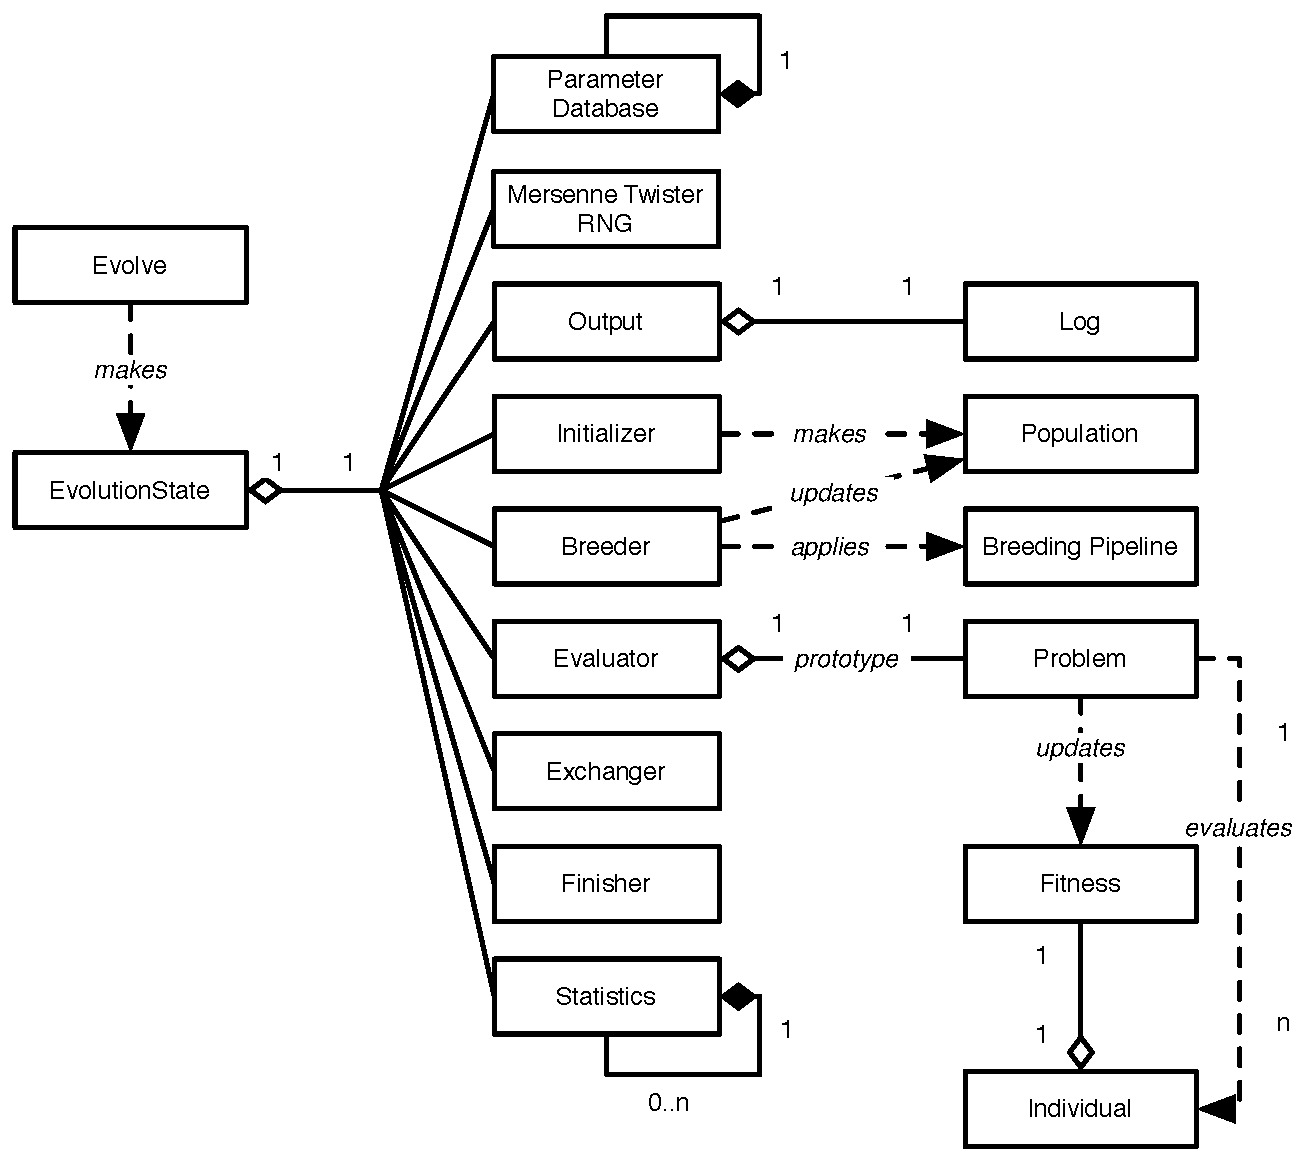
\includegraphics[width=5in]{Operators.pdf}
\end{center}
\caption{Top-Level operators and utility facilities in EvolutionState, and their relationship to certain state objects.  A repeat of Figure \ref{Operators}.  Compare to Figure \ref{SteadyState}.}
\label{Operators2}
\end{figure}


If you peek inside \class{ec.EvolutionState}, you will find a number of objects, as shown in Figure \ref{Operators2}:

\begin{itemize}
\item Some familiar objects, placed there by \class{ec.Evolve} after it created the \class{ec.EvolutionState}: the {\bf Parameter Database, Output,} and array of {\bf Random Number Generators}.  Additionally, the number of {\bf breeding threads} and {\bf evaluation threads} (and various checkpoint and job stuff, not shown below):

\java{%
public ec.util.ParameterDatabase parameters;\\
public ec.util.MersenneTwisterFast[] random;\\
public ec.util.Output output;\\
public int breedthreads;\\
public int evalthreads;
}

\item A {\bf Population}, which holds the individuals in the evolutionary process; plus the current {\bf generation} (iteration) of the evolutionary process and the total {\bf number of generations} to run (how or whether these last two variables are used depends on the evolutionary process in question):

\java{%is 
public ec.Population population;\\
public int generation;\\
public int numGenerations;
}

\item An {\bf Initializer}, whose job is to create the initial \class{ec.Population} at the beginning of the run, and a {\bf Finalizer}, whose job is to clean up at the very end of the run.

\java{%
public ec.Initializer initializer;\\
public ec.Finalizer finalizer;
}

\item An {\bf Evaluator}, whose job is assign quality assessments (fitnesses) to each member of the Population, and a {\bf Breeder}, whose job is to produce a new Population from the previous-generation's Population through some collection of selection and modification operators.

\java{%
public ec.Evaluator evaluator;\\
public ec.Breeder breeder;
}

\item An {\bf Exchanger}, which optionally exports Population members to other ECJ processes, or imports ones to add to the Population.  And finally, a {\bf Statistics} object, whose methods are called at many points in the run to output statistics on the current run performance.

\java{%
public ec.Exchanger exchanger;\\
public ec.Statistics statistics;
}

\end{itemize}

\section{Common Patterns}
\label{patterns}

Most of ECJ's classes follow certain patterns which you'll see many times, so it's useful to review them here.

\subsection{Setup}  Nearly all classes adhere to the \class{ec.Setup} interface.  This interface is \class{java.io.Serializable} (which is why ECJ can serialize all its objects) and defines a single additional method:

\begin{methods}{ec.Setup}
\mthd{public void setup(EvolutionState {\it state}, Parameter {\it base})}
Constructs the Setup object from the Parameter Database using {\it base} as the primary parameter base.  Nearly all ECJ classes implement this method.
\end{methods}

ECJ objects are born from ECJ's Parameter Database, which constructs them with the default (no-argument) constructor.  Then they have \method{setup(...)} called on them, and are expected to construct themselves by loading parameters as necessary from the Parameter Database (\method{state.parameters}), using the provided Parameter base.  Thus the \method{setup(...)} method is, for all intents and purposes, the constructor.

When implementing \method{setup(...)} always call \method{super.setup(...)} if a superclass exists.

\subsection{Singletons and Cliques}
\label{clique}
  Singletons (\class{ec.Singleton}) are Setups which create a single instance and that's it.  For example, \class{ec.EvolutionState} is a Singleton, as are \class{ec.Initializer}, \class{ec.Finalizer}, \class{ec.Evaluator}, \class{ec.Breeder}, \class{ec.Exchanger}, and \class{ec.Statistics}.  Singletons are generally meant to be globally accessible.

Though Singleton are single objects, Cliques (\class{ec.Clique}) are objects for which only a small number (but usually more than 1) are created.  Cliques are also generally meant to be globally accessible.  Most Cliques have a globally accessible registry of some sort in which all Clique members can be found.

Because they are global, Prototypes and Singletons usually are set up from a single parameter base (the one provided by \method{setup(..)}).

\subsection{Prototypes}   Prototypes (\class{ec.Prototype}) are by far the most common objects in ECJ.  Prototypes are Setups which follow the following design pattern: only one instance is loaded from the Parameter Database and set up; this object is the {\it prototype}.  Then many objects are created by {\it deep cloning} the prototype.  One example of a Prototype is an Individual (\class{ec.Individual}): a single prototypical Individual is created when ECJ starts up; and further Individuals are deep cloned from this prototype to fill Populations.

Because they can are deep cloned, Prototypes implement the \class{java.lang.Cloneable} interface, so you must implement the method:

\begin{methods}{ec.Prototype}
\mthd{public Object clone()}
Deep-clones the object.  Implemented by all Prototypes.  Must call super.clone(), possibly catching a thrown \class{CloneNotSupportedException}.
\end{methods}

Unlike Singletons and Cliques, Prototypes also usually have {\it two} parameter bases: the primary base provided by \method{setup(...)}, and a default base.  As a result, Prototypes must implement a method which can be called to provide this default base:

\begin{methods}{ec.Prototype}
\mthd{public ec.util.Parameter defaultBase()}
Returns the default base for the Prototype.
\end{methods}

The standard way to implement this method is to consult a special {\bf defaults class} in the Parameter's Java package.  For example, in the \package{ec.simple} package the defaults class is \class{ec.simple.SimpleDefaults}.  Here's the entirety of this class:

\vbox{
\small\begin{verbatim}
    public final class SimpleDefaults implements ec.DefaultsForm 
        {
        public static final String P_SIMPLE = "simple";
        public static final Parameter base()  {  return new Parameter(P_SIMPLE); }
        }
\end{verbatim}
}

The Parameter returned by \method{base()} here provides {\bf package default base} for the \package{ec.simple} package.  Now consider \class{ec.simple.SimpleFitness}, a Prototype in this package.  This class implements the \method{defaultBase()} method like this:

\vbox{
\small\begin{verbatim}
    public static final String P_FITNESS = "fitness";
    public Parameter defaultBase()
        {
        return SimpleDefaults.base().push(P_FITNESS);
        }
\end{verbatim}
}

Thus, as a result the default parameter base for \class{ec.simple.SimpleFitness} is \parameter{simple.fitness}.

\subsection{The Flyweight Pattern}\label{flyweight}  Many Prototypes follow what is commonly known as the {\bf flyweight pattern}.  Prototypes are often great in number and Java is a memory hog: so it's helpful for groups of Prototypes to place shared information common to them in a single central location rather than keep copies of their own.  For various reasons (particularly because it's hard to do serialization) ECJ doesn't use static variables to store this common information.  Instead groups of Prototypes often all point to a special object which contains information common to all of them.  For example, instances of \class{ec.Individual}, in groups, typically share a common \class{ec.Species} which contains information common to them.  At any particular time there may be several such groups of Individuals, each with a {\it different} Species.

\subsection{Groups}
\label{ec.Group}
Groups are similar to Prototypes in that a single object is loaded from the Parameter Database and further objects are created by a cloning procedure.  Groups are likewise \class{java.lang.Cloneable}.  However, Groups are different in that there is no prototype per se: the object loaded from the Parameter Database isn't held in reserve but is actively used.  It must not just clone another object, but actually create a new, fresh, clean object ready to be used.  This is done by implementing the method:

\begin{methods}{ec.Group}
\mthd{public ec.util.Parameter emptyClone()}
Returns a pristine, new clone of the Group which has been emptied of members.
\end{methods}

This method is normally implemented by cloning the object, cleaning out the clone, and returning it in the same pristine state that it would be if it had been created directly from the Parameter Database.  At present there are only a few ECJ objects which implement \class{Group}: namely, \class{ec.Population}, \class{ec.Subpopulation}, and certain specialized subclasses of \class{ec.Subpopulation}.

\begin{figure}
\begin{center}
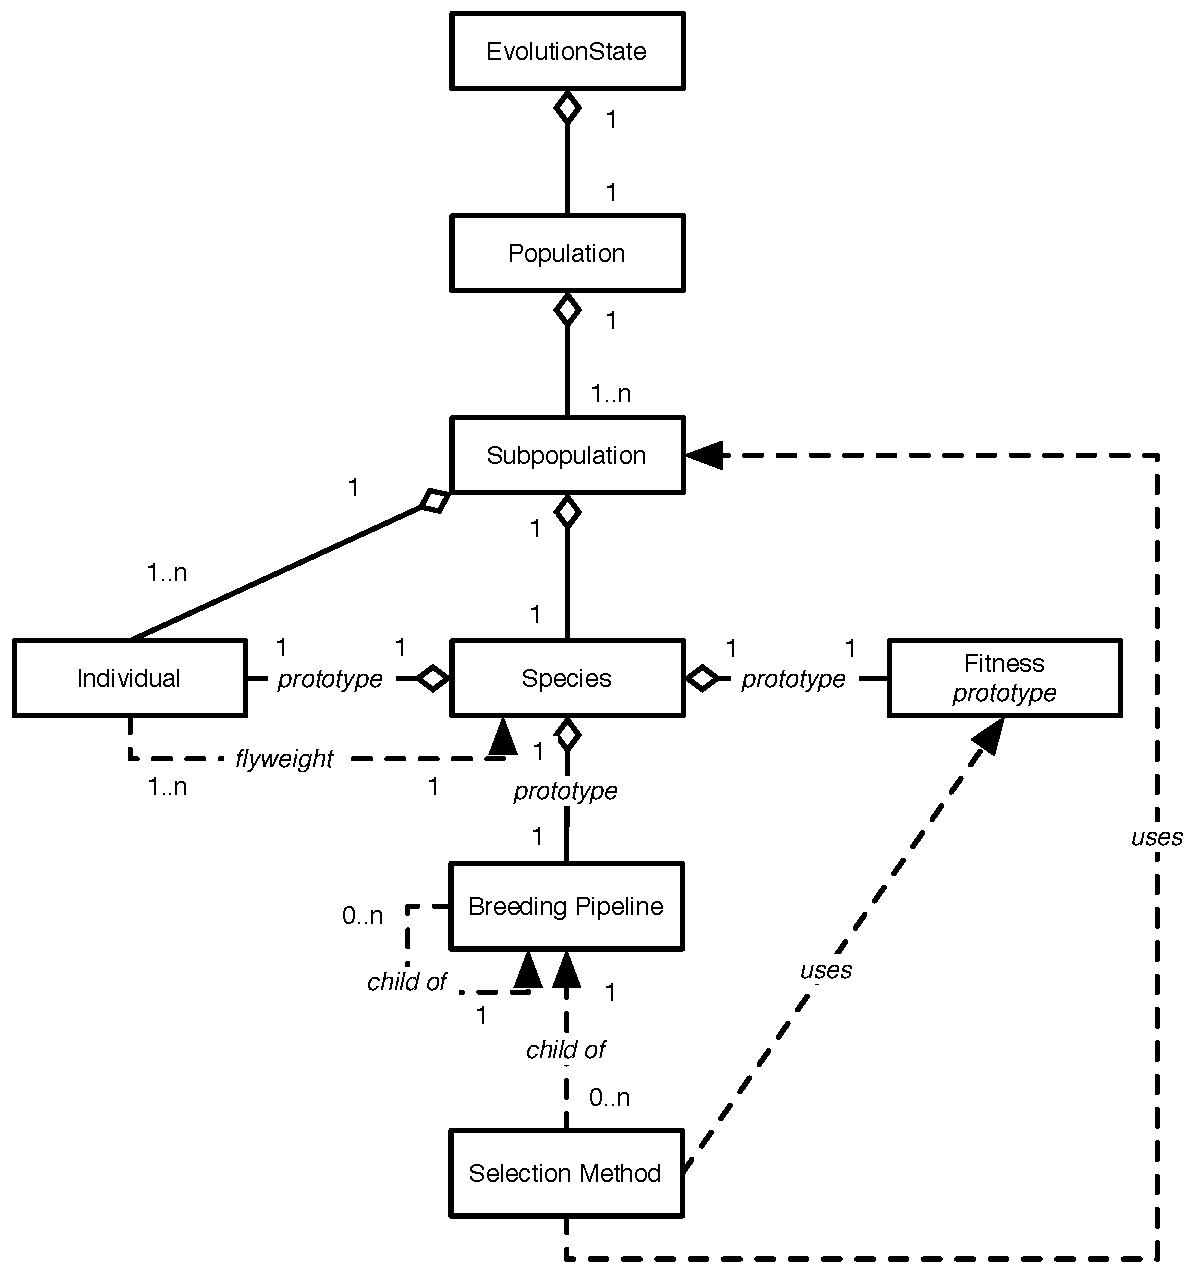
\includegraphics[width=4.7in]{StateObjects.pdf}
\end{center}
\caption{Top-Level data objects used in evolution.  A repeat of Figure \ref{StateObjects}.}
\label{StateObjects2}
\end{figure}

\section{Populations, Subpopulations, Species, Individuals, and Fitnesses}
\label{populationsetc}

Populations, Subpopulations, and Individuals are the ``nouns'' of an evolutionary system, and Fitnesses are the ``adjectives''.  They're pretty central to the operation of any evolutionary or sample-based stochastic search algorithm.

In ECJ, an {\bf individual} is a candidate solution to a problem.  Some \(M\) Individuals are grouped together into a sample of solutions known as a {\bf subpopulation}.  Some \(N\) subpopulations are grouped together into the system's {\bf population}.  There's only one population per evolutionary process.  The most common scenario is for ECJ to have \(M\) individuals grouped into a single subpopulation, which then is the sole member of ECJ's population.  However, coevolutionary algorithms (Section~\ref{ec.coevolve}) typically have \(N>1\) subpopulations: as do a special and little-used internal island model scheme (see Section~\ref{ec.exchange}).\footnote{Because these two techniques use the subpopulations in different ways, they cannot be used together (a rare situation in ECJ).}

Usually ECJ's population is an instance of the class \class{ec.Population} and its subpopulations are instances of the class \class{ec.Subpopulation}.  Both of these are Groups. Let's say that there's a single subpopulation, which must contain 100 individuals.  We're express this as follows:

\params{%
pop = ec.Population\\
pop.subpops = 1\\
pop.subpop.0 = ec.Subpopulation\\
pop.subpop.0.size = 100
}

Obviously further subpopulations would be \parameter{pop.subpop.1}, \parameter{pop.subpop.2}, etc.  The population is found in an instance variable in the EvolutionState:  

\java{%
    public Population population;
}

The Population is little more than an array of Subpopulations.  To get Subpopulation 0, with the EvolutionState being \variable{state}, you'd say:

\java{
Subpopulation theSubpop = state.population.subpops[0];
}

Subpopulations themselves contain arrays of individuals.  To get Individual 15 of Subpopulation 0, you'd say:

\java{
Individual theIndividual = state.population.subpops[0].individuals[15];
}

In addition to an array of individuals, each subpopulation contains a {\bf species} which defines the individuals used to fill the subpopulation, as well as their fitness and the means by which they are modified.  Subpopulations also contain some basic parameters for creating initial individuals, though the procedure is largely handled by Species.\footnote{You might be asking: if Species are responsible for making individuals, why are Subpopulations involved at all?  A very good question indeed.}  We'll get to creation and modification later.

Species have an odd relationship to Individuals and to Subpopulations.  First recall the Flyweight pattern in Section~\ref{flyweight}.  Individuals are related to a common Species using the Flyweight pattern: they use Species to store a lot of common information (how to modify themselves, for example).  Ordinarily you'd think that the Subpopulation would be a good place for this storage.  However different Subpopulations can share the same Species.  This allows you to, for example, have one Species guide an entire evolutionary run that might have twenty Subpoulations in it.\footnote{Granted, this isn't very common.}  The species of Subpopulation 0 may be found here:

\java{
Species theSpecies = state.population.subpops[0].species;
}

A Species contains three major elements: first, the {\bf prototypical Individual} for Subpopulations which use that Species. Recall that Individuals are Prototypes and new ones are formed by cloning from a prototypical individual held in reserve.  This ``queen bee'' individual, so to speak, is found here:

\indent\hspace{1.25em}\vbox{
\small\begin{verbatim}
Individual theProto = state.population.subpops[0].species.i_prototype;
\end{verbatim}
}

A Species also contains a {\bf prototypical Fitness} object.  In ECJ {\it fitnesses} are separate from {\it individuals}.  Individuals define the candidate solution, and Fitnesses define how well it has performed.  Like Individuals, Fitnesses are also Prototypes.  The prototypical Fitness for Subpopulation 0 may be found here:

\indent\hspace{1.25em}\vbox{
\small\begin{verbatim}
Fitness theProtoFitness = state.population.subpops[0].species.f_prototype;
\end{verbatim}
}

The Species class you pick is usually determined by the kind of Individual you pick, that is, by the kind of representation of your solution.  You define the class of the Species for Subpopulation 0, and its prototypical Fitness and prototypical Individual, as follows.  For example, let's make Individuals which are arrays of integers, and a simple Fitness common to many evolutionary algorithms:

\params{%
pop.subpop.0.species = ec.vector.IntegerVectorSpecies\\
pop.subpop.0.species.ind = ec.vector.IntegerVectorIndividual\\
pop.subpop.0.species.fitness = ec.simple.SimpleFitness
}

By way of explanation, \class{IntegerVectorIndividual}, along with various other ``integer'' vector individuals like \class{LongVectorIndividual}, \class{ShortVectorIndividual}, and \class{ByteVectorIndividual}, requires an \class{IntegerVectorSpecies}.  And \class{ec.simple.SimpleFitness} is widely used for problems such as Genetic Algorithms or Evolution Strategies.  The prototypical Individual is never assigned a Fitness (it's null).  But once assembled in a Subpopulation, each Individual has its very own Fitness.  To get the Fitness of individual 15 in Subpopulation 0, you'd say:

\indent\hspace{1.25em}\vbox{
\small\begin{verbatim}
Fitness theFitness = state.population.subpops[0].individuals[15].fitness;
\end{verbatim}
}

Last, a Species contains a {\bf prototypical Breeding Pipeline} to modify individuals.  We'll get to that in Section~\ref{breeders}.

Since they're Prototypes, Individuals, Fitnesses, and Species all have default bases.  We'll talk about the different kinds of Individuals, Fitnesses, and Species later, plus various default bases for them.

\subsection{How Species Make Individuals}
\label{ec.Species}

Species have two ways to create new individuals: from scratch, or reading from a stream.  To generate an individual from scratch, you can call (in \class{ec.Species}):

\begin{methods}{ec.Species}
\mthd{public Individual newIndividual(EvolutionState \textit{state}, int \textit{thread})}
Returns a brand new, randomized Individual.
\end{methods}

The default implementation of this method simply clones an Individual from the prototype and returns it.  Subclasses of Species override this to randomize the Individual in a fashion appropriate to its representation.

Another way to create an individual is to read it from a binary or text stream.  \class{ec.Species} provides two methods for this:

\begin{methods}{ec.Species}
\mthd{public Individual newIndividual(EvolutionState \textit{state}, LineNumberReader \textit{reader}) throws IOException}
Produces a new individual read from the stream.
\mthd{public Individual newIndividual(EvolutionState \textit{state}, DataInput \textit{input}) throws IOException}
Produces a new individual read from the given DataInput.
\end{methods}

These methods create Individuals by cloning the prototype, then calling the equivalent \method{readIndividual(...)} method in \class{ec.Individual}.  See Section~\ref{ec.Individual} for more information on those methods.

\subsection{Reading and Writing Populations and Subpopulations}
\label{ec.Population}
\label{ec.Subpopulation}

Populations and Subpopulations have certain predefined methods for reading and writing, which you should know how to use.  If you subclass Population or Subpopulation (relatively rare) you may need to reimplement these methods.  Population's methods are:

\java{%
public void printPopulationForHumans(EvolutionState state, int log);\\
public void printPopulation(EvolutionState state, int log);\\
public void printPopulation(EvolutionState state, PrintWriter writer);\\
public void readPopulation(EvolutionState state, LineNumberReader reader)\\
\hsp{\fill}throws IOException;\\
public void writePopulation(EvolutionState state, DataOutput output)\\
\hsp{\fill}throws IOException;\\
public void readPopulation(EvolutionState state, DataInput input)\\
\hsp{\fill}throws IOException;
}

Subpopulation's methods are nearly identical:

\paragraph{In Subpopulation:}
\java{%
public void printSubopulationForHumans(EvolutionState state, int log);\\
public void printSubopulation(EvolutionState state, int log);\\
public void printSubopulation(EvolutionState state, PrintWriter writer);\\
public void readSubopulation(EvolutionState state, LineNumberReader reader)\\
\hsp{\fill}throws IOException;\\
public void writeSubopulation(EvolutionState state, DataOutput output)\\
\hsp{\fill}throws IOException;\\
public void readSubopulation(EvolutionState state, DataInput input)\\
\hsp{\fill}throws IOException;
}

These methods employ similar methods in \class{ec.Individual} to print out, or read, Individuals.  Those methods are discussed next in Section~\ref{ec.Individual}.

The first Population method, \method{printPopulationForHumans(...)}, prints an entire population to a log in a form pleasing to the human eye. It begins by  printing out the number of subpopulations, then prints each Subpopulation index and calls \method{printSubpopulationForHumans(...)} on each Subpopulation in turn.  \method{printPopulationForHumans(...)} then prints out the number of individuals, then for each Individual it prints the Individual index, then calls \method{printIndividualForHumans} to print the Individual.  Overall, it looks along these lines:

\vbox{
\small\begin{verbatim}
Number of Subpopulations: 1
Subpopulation Number: 0
Number of Individuals: 1000
Individual Number: 0
Evaluated: T
Fitness: 0.234
 -4.97551104730313 -1.7220830524609632 1.7908415218297096
 2.3277606156190496 3.5616099573877404 -3.8002895023118617 
Individual Number: 1
Evaluated: T
Fitness: 4.91235
 3.1033182498148575 -3.613847679151146 -0.562978505270439
 -2.860926011046968 1.9007479097991151 -3.051348823625001 
...
 \end{verbatim}
}

The next two Population methods, both named \method{printPopulation(...)}, print an entire population to a log in a form that can be (barely) read by humans but can also be read back in perfectly by ECJ, resulting in identical Populations  These operate similarly to \method{printPopulationForHumans(...)}, except that various data types are emitted using \method{ec.util.Code} (Section~\ref{ec.util.Code}).


\vbox{
\small\begin{verbatim}
Number of Subpopulations: i1|
Subpopulation Number: i0|
Number of Individuals: i1000|
Individual Number: i0|
Evaluated: F
Fitness: f0|0.0|
i6|d4600627607395240880|0.3861348728170766|d4616510324226321041|4.284844300646584|
d4614576621171274054|3.2836854885228233|d4616394543356495435|4.182010230653371|
Individual Number: i1|
Evaluated: F
Fitness: f0|0.0|
i6|d4603775819114015296|0.6217914592919627|d4612464338011645914|2.345643329183969|
d-4606767824441912859|-4.368233761797886|d4616007477858046134|3.919113503960115|
...
 \end{verbatim}
}

The Population method \method{readPopulation(..., LineNumberReader)} can read in this mess to produce a Population.  It in turn does its magic by calling the equivalent method in Subpopulation.

The last two methods, \method{writePopulation(...)} and \method{readPopulation(..., DataInput)}, read and write Populations (or Subpopulations) to binary files.

\subsection{About Individuals}
\label{ec.Individual}

Individuals have four basic parts:

\begin{itemize}
\item The Individual's fitness.

\java{%
public Fitness fitness;
}

\item The Individual's species.

\java{%
public Species species;
}

\item Whether the individual has been evaluated and had its Fitness set to a legal value yet.\footnote{Why isn't this in the Fitness object?  Another excellent question.}

\java{%
public boolean evaluated;
}

\item The representation of the Individual.  This could be anything from an array to a tree structure\,---\,representations of course vary and are defined by subclasses.  We'll talk about them later.
\end{itemize}

\subsubsection{Implementing an Individual}  For many purposes you can just use one of the standard ``off-the-rack'' individuals\,---\, vector individuals, genetic programming tree individuals, ruleset individuals\,---\, but if you need to implement one yourself, here are some methods you need to be aware of.  First off, Individuals are Prototypes and must override the \method{clone()} method to deep-clone themselves, including deep-cloning their representation and their Fitness, but not their Species (which is just pointer-copied).  Individuals must also implement the \method{setup(...)}, and \method{defaultBase()} methods.  Additionally, Individuals have a number of method which either should or must be overridden.  Let's start with the ``must override'' ones:

\java{%
public abstract int hashCode();\\
public abstract boolean equals(Object individual);
}

These two standard Java methods enable hashing by value, which allows Subpopulations to remove duplicate Individuals.  \method{hashCode()} must return a hashcode for an individual based on value of its representation.  \method{equals(...)} must return true if the Individual is identical to the other object (which in ECJ will always be another Individual).

The next two methods are optional and may not be appropriate depending on your representation:

\java{%
public long size();\\
public double distanceTo(Individual other);
}

\method{size()} returns an estimate of the size of the individual.  The only hard-and-fast rule is that 0 is the smallest possible size (and the default returned by the method).  Size information is largely used by the \package{ec.parsimony} package (Section~\ref{ec.parsimony}) to apply one of several parsimony pressure techniques.

\method{distanceTo(...)} returns an estimate of the distance, in some metric space, of the Individual to some other Individual of the same type.  In the future this method may be used for various crowding or niching methods.  At present no package uses it, though all vector individuals implement it.  The default implementation returns 0 if the other Individual  is identical, else \variable{Double.POSITIVE\_INFINITY}.

Last come a host of functions whose purpose is to read and write individuals.  You've seen this pattern before in Section~\ref{ec.Population}.  Some of these are important to implement; others can wait if you're in a hurry to get your custom Individual up and running.

\java{%
public void printIndividualForHumans(EvolutionState state, int log);\\
public void printIndividual(EvolutionState state, int log);\\
public void printIndividual(EvolutionState state, PrintWriter writer);\\
public void readIndividual(EvolutionState state, LineNumberReader reader)\\
\hsp{\fill}throws IOException;\\
public void writeIndividual(EvolutionState state, DataOutput output)\\
\hsp{\fill}throws IOException;\\
public void readIndividual(EvolutionState state, DataInput input)\\
\hsp{\fill}throws IOException;
}

These six methods only need to be overridden in certain situations, and in each case there's another method which is typically overridden instead.  Here's what they do:

\begin{itemize}
\item \method{printIndividualForHumans(...)} prints an individual, whether it's been evaluated, and its fitness, out a log in a way that's pleasing and useful for real people to read.    Rather than override this method, you probably should instead override this method:

\java{%
public String genotypeToStringForHumans();
}

... which should return the representation of the individual in a human-pleasing fashion.  Or, since \method{genotypeToStringForHumans()} by default just calls \method{toString()}, you can just override:

\java{%
public String toString();
}

Overriding one or both of these methods is pretty important: otherwise Statistics objects will largely be printing your individuals as gibberish.  Here's a typical output of these methods:

\vbox{
\small\begin{verbatim}
Evaluated: T
Fitness: 0.234
 -4.97551104730313 -1.7220830524609632 1.7908415218297096
 2.3277606156190496 3.5616099573877404 -3.8002895023118617 
 \end{verbatim}
}

\item Both \method{printIndividual(...)} methods print an individual, and its fitness, out in a way that can be perfectly read back in again with \method{readIndividual(...)}, but which can also be parsed by humans with some effort.    Rather than override this method, you probably should instead override this method:

\java{%
public String genotypeToString();
}

This method is important to implement only if you intend to write individuals out to files in such a way that you can load them back in later.  If you don't implement it, \method{toString()} will be used, which probably won't be as helpful.  This returns a String which can be parsed in again in the next method.  Note that you need to write an individual out so that it can {\it perfectly} be read back in again as an identical individual.  How do you do this?  ECJ's classes by default all use the aging and idiosyncratic package \method{ec.util.Code} package developed long ago for this purpose, but which still works well.  See Section~\ref{ec.util.Code}.

Here's a typical output of these methods (note the use of \method{ec.util.Code}):

\vbox{
\small\begin{verbatim}
Evaluated: F
Fitness: f0|0.0|
i6|d4600627607395240880|0.3861348728170766|d4616510324226321041|4.284844300646584|
d4614576621171274054|3.2836854885228233|d4616394543356495435|4.182010230653371|
 \end{verbatim}
}


\item \method{readIndividual(..., LineNumberReader)} reads an individual, and its fitness, in from a LineNumberReader.  The stream of text being read is assumed to have been generated by \method{printIndividual(...}.  Rather than override this method, you probably should instead override this method:

\java{%
protected void parseGenotype(EvolutionState state, LineNumberReader reader)\\
\hsp{\fill}throws IOException;\\
}

This returns a String which can be parsed in again in the next method.  Note that you need to write an individual out so that it can {\it perfectly} be read back in again as an identical individual.  How do you do this?  ECJ's classes by default all use the aging and idiosyncratic package \method{ec.util.Code} package developed long ago for this purpose, but which still works well.  See Section~\ref{ec.util.Code}.  You only need to override this method if you plan on reading individuals in from files (by default the method just throws an error).

\item The last two methods (\method{writeIndividual(...)} and \method{readIndividual(..., DataInput)} read and write an individual, including its representation, fitness and evaluated flag, in a purely binary fashion to a stream.  Don't write the Species.  It's probably best instead to override the following methods to just read and write the genotype:

\java{%
public void writeGenotype(EvolutionState state, DataOutput output)\\
\hsp{\fill}throws IOException;\\
public void readGenotype(EvolutionState state, DataInput input)\\
\hsp{\fill}throws IOException;\\
}

These methods are probably only important if you plan on using ECJ's distributed facilities (distributed evaluator, island models).  The default implementations of these methods throw exceptions.

\end{itemize}

\subsection{About Fitnesses}
\label{ec.Fitness}

Fitnesses are separate from Individuals, and various Fitnesses can be used depending on the demands of the evolutionary algorithm.  The most common Fitness is \class{ec.simple.SimpleFitness}, which represents fitness as a single number from negative infinity to positive infinity, where larger values are ``fitter''.  Certain selection methods (notably fitness proportionate selection) require that the fitness be non-negative; and ideally between 0 and 1 inclusive.

There are other Fitness objects.  For example, there are various multiobjective fitnesses (see Section~\ref{ec.multiobjective}), in which the fitness value is not one but some \(N\) numbers, and either higher or lower may be better depending on the algorithm.  Other Fitnesses, like the one used in genetic programming (Section~\ref{ec.gp}), maintain a primary Fitness statistic and certain auxiliary ones.
 

You probably won't need to implement a Fitness object.  But you may need to use some of the methods below.  Fitnesses are Prototypes and so must implement the \method{clone()} (as a deep-clone), \method{setup(...)}, and \method{defaultBase()} methods.  Fitness has four additional required methods:

\java{%
public abstract float fitness();\\
public abstract boolean isIdealFitness();\\
public abstract boolean equivalentTo(Fitness other);\\
public abstract boolean betterThan(Fitness other);
}

The first method, \method{fitness()}, should return the fitness cast into a value from negative infinity to positive infinity, where higher values are better.  This is used largely for fitness-proportionate and similar selection methods.  If there is no appropriate mechanism for this, you'll need to fake it.  For example, multiobjective fitnesses might return the maximum or sum over their various objectives. 

The second method, \method{isIdealFitness()}, returns true if the fitness in question is the best possible.  This is largely used to determine if it's okay to quit.  It's fine for this method to always return false if you so desire.

The third and fourth methods compare against another fitness object, of the same type.  The first returns true if the two Fitnesses are in the same equivalence class: that is, neither is fitter than the other.  For simple fitnesses, this is just equality.  For multiobjective fitnesses this is Pareto-nondomination of one another.  The second method returns true if the Fitness is superior to the one provided in the method.  For simple fitnesses, this just means fitter.  For multiobjective fitnesses this implies Pareto domination.

Fitnesses also have similar printing facilities to Individuals:\footnote{Starting to get redundant?  Sorry about that.}

\java{%
public void printFitnessForHumans(EvolutionState state, int log);\\
public void printFitness(EvolutionState state, int log);\\
public void printFitness(EvolutionState state, PrintWriter writer);\\
public void readFitness(EvolutionState state, LineNumberReader reader)\\
\hsp{\fill}throws IOException;\\
public void writeFitness(EvolutionState state, DataOutput output)\\
\hsp{\fill}throws IOException;\\
public void readFitness(EvolutionState state, DataInput input)\\
\hsp{\fill}throws IOException;\\
}

As usual: the first method, \method{printFitnessForHumans(...)}, prints a Fitness in a way pleasing for humans to read.  It simply prints out the result of the following method (which you should override instead if you ever need to):

\java{%
public String fitnessToStringForHumans();
}

The default implementation of \method{fitnessToString()} simply calls:

\java{%
public String toString();
} 

The next two methods, both named \method{printFitness(...)}, prints a Fitness in a way that can be (barely) read by humans, and can be read by ECJ to produce an identical Fitness to the original.  These methods just print out the result of the following method (which you should override instead if you ever need to):

\java{%
public String fitnessToString();
}

The default implementation of this method calls \method{toString()}, which is almost certainly wrong.  But all the standard Fitness subclasses implement it appropriately using the \class{ec.util.Code} tools (Section~\ref{ec.util.Code}).

The method \method{readFitness(..., LineNumberReader)} reads into ECJ a Fitness written by these last two printers.  Finally, the last two methods, \method{writeFitness(...)} and \method{readFitness(..., DataInput)}, read and write the Fitness in a binary fashion.  The default implementation of these methods throws an error, but all standard subclasses of Fitness implement them properly.

Fitnesses have one auxiliary variable:

java{%
public int trials;
}

This variable is used by the coevolutionary processes (see Section \ref{ec.coevolve}) to keep track of the number of trials used to compute the Fitness value.  Outside of coevolution it's presently unused.  Ultimately the variable doesn't matter once the Fitness has been computed.

\section{Initializers and Finishers}
\label{ec.Initializer}
\label{ec.Finisher}

The {\bf Initializer} is called at the beginning of an evolutionary run to create the initial population.  The {\bf Finisher} is called at the end of a run to clean up.  In fact, it's very rare to use any Finisher other than \class{ec.simple.Finisher}, which does nothing at all.  So nearly always you'll have this:

\params{%
finish = ec.simple.SimpleFinisher
}

Initializers vary largely based on representation, but not for the reason you think.  Initializers generally don't need to know anything about the representation of an individual in order to construct it.  Instead, certain representations require a lot of pieces which need to be in a central repository (they're Cliques).  For example, the genetic programming facility (Section~\ref{ec.gp}) has various {\it types}, {\it function sets}, {\it tree constraints}, {\it node constraints}, etc.  It's not in ECJ's style to store these things as static variables because of the difficulty it presents for serialization.  Instead ECJ needed a global object to hold them, and Initializers were chosen for that task.  It's probably not been the smartest of decisions: Finishers (which have historically had little purpose) could have been recruited to the job, or some generic type repository perhaps.  As it stands, Initializers aren't an optimal location, but there it is.\footnote{This makes it problematic to have both a ``rule'' representation and a genetic programming representation in the same run without a little hacking, since both require their own Initializer.  Perhaps this might be remedied in the future.}

Unless you're doing genetic programming (\package{ec.gp}) or using the \package{ec.rule} package, you'll probably use a 
\class{ec.simple.SimpleInitializer}:

\params{%
init = ec.simple.SimpleInitializer
}

ECJ's generational\footnote{ECJ's Steady State evolution mechanism has a different initialization procedure.  See Section~\ref{ec.steadystate} for more information.} initialization procedure goes like this:

\begin{enumerate}
\item The EvolutionState asks the Initializer to build a Population by calling:

\java{%
population = state.initializer.initialPopulation(state, 0);
}

The 0 is thread index 0: this portion of the code is single-threaded.

\item The Initializer then creates and sets up a Population by calling the following on itself.  It then tells the Population to populate itself with individuals:

\java{%
Population pop = setupPopulation(state, 0);\\
pop.populate(state, 0);
}

Why break this out?  Because there are a few EvolutionState subclasses which don't want to populate the population immediately or at all\,---\,they just want to set it up.  For example, steady state evolution sets up a Population but may only gradually fill it with initial population members.  In this case, the steady state system will just call \method{setupPopulation(...)} directly, bypassing \method{initialPopulation(...)}.

\item The Population's \method{populate(...)} method is straightforward: it calls \method{populate(...)} in turn on each Subpoulation in the Population's subpopulation array.

\item A Subpopulation's \method{populate(...)} method usually works like this.  First, it determines if it should create new individuals from scratch or if it should fill its array by reading Individuals from a file.  This is determined by (as usual) a parameter!  If Subpopulation 0 should be read in from the file \file{/tmp/population.in}, the parameter setting would be:

\params{%
pop.subpop.0.file = /tmp/population.in
}

Subpopulation will try to read individuals from this file using their \method{readIndividual(..., LineNumberReader)} method.   However if the number of individuals in the file doesn't match the size of the Subpopulation, the Subpopulation will be resized to match the file, deleting the original Individuals.  Subpopulation will then read individuals using the \method{newIndividual(..., LineNumberReader)} method in \class{ec.Species} (slightly less efficient).  (See Section~\ref{ec.Species}).

If no file is provided, the Subpopulation assumes that it is generating individuals from scratch.  This is by far the most common case.  To do this, Subpopulation generates new individuals using the standard \method{newIndividual(...)} method in \class{ec.Species} (see Section~\ref{ec.Species}).  ECJ can also check to make sure that the Subpopulation does not produce duplicate individuals, if you set the following parameter (in this case, in Subpopulation 0):

\params{%
pop.subpop.0.duplicate-retries = 100
}

The default value is no retries.

This says that if the Subpopulation creates a duplicate individual, it will try up to 100 times to replace it with a new, original individual.  After that it will give up and use the duplicate individual. 

\end{enumerate}


















\section{Evaluators and Problems}
\label{ec.Evaluator}

ECJ evaluates (assesses the fitness of) Individuals in a Population by passing it to an \class{ec.Evaluator}.  Various evolutionary algorithms and other stochastic search algorithms have their own special kinds of Evaluators.  Evaluators perform this fitness assessment by cloning one or more {\bf Problems}, discussed in the next Section, and asking these Problems to evaluate the individuals on their behalf.  Evaluators hold the prototypical Problem here:

\java{%
public Problem p\_problem;
}

This problem is loaded from parameters.  For example, to specify that we will use the Artificial Ant Problem to test our genetic programming Individuals, we'd say:

\params{%
eval.problem = ec.app.ant.Ant
}

The basic Evaluator is \class{ec.simple.SimpleEvaluator}.  This class evaluates a Population first by determining how many threads to use.  To use four threads (for example), we say:

\params{%
evalthreads = 4
}

The default value is a single thread.

Recall from Section~\ref{threads} that his will require at least four random number generator seeds, for example:

\params{%
seed.0 = 1234\\
seed.1 = -503812\\
seed.2 =  992341\\
seed.3 = -16723
}

When evaluating a Population, \class{ec.simple.SimpleEvaluator} will construct \(N\) Problems cloned from the Problem prototype.   Then, for each Subpopulation, the Evaluator will break the Subpopulation into \(N\) chunks (one per thread), and assign each chunk to a different Problem instance.  This enables the Population to be evaluated in parallel.  Most commonly, we just set \(N=1\). 

Certain Evaluator methods are required.  The primary method an Evaluator must implement is

\java{%
public abstract void evaluatePopulation(EvolutionState state);
}

This method must take the Population (that is, \variable{state.population}) and evaluate all the individuals in it in the fashion expected by the stochastic search algorithm being employed.   Additionally, an Evaluator must implement the method

\java{%
public abstract boolean runComplete(EvolutionState state);
}

\noindent ... which returns \variable{true} if the Evaluator believes the process has reached a terminating state.  Typically this is done by scanning through the Population and determining if any of the Individuals have ideal fitnesses.  If you don't want to be bothered, it's fine to have this method always return \variable{false}.

\subsection{Problems}
\label{ec.Problem}

Evaluators assess the fitness of individuals typically by creating one or more Problems and handing them chunks of Subpopulations to evaluate.  There are two ways that an Evaluator can ask a Problem to perform evaluation:

\begin{itemize}

\item For each Individual, the Evaluator can call the Problem's {\it evaluation} method.  This method varies depending on the kind of Problem.  Problems which adhere to \class{ec.simple.SimpleProblemForm}\,---\,by far the most common situation\,---\,use the following method:

\java{%
public void evaluate(EvolutionState state, Individual ind,\\
\hsp{\fill}int subpopulation, int threadnum);
}

When this approach is taken, the Problem must assign a fitness immediately during the \method{evaluate(...)} method.  In practice, ECJ doesn't do this all that much.

\item  The more common approach allows a Problem to perform fitness evaluation in bulk.  In this approach, the Evaluator will first call the following method once:

\java{%
public void prepareToEvaluate(EvolutionState state, int thread);
}

This signals to the Problem that it must prepare itself to begin evaluating a series of Individuals, and then afterwards assign fitness to all of them.    Next the Evaluator calls the Problem's {\it evaluation} method for each Individual, typically using the method \method{evaluate(...)} as before.  Finally, the Evaluator calls this method:

\java{%
public void finishEvaluating(EvolutionState state, int thread);
}

Using this approach, the Problem is permitted to delay assigning fitness to Individuals until \method{finishEvaluating(...)} is called.

\end{itemize}

When ECJ is preparing to exit various Statistics objects sometimes construct a Problem in order to re-evaluate the fittest Individual of the run, solely to have such evaluation print out useful information to tell the user how the Individual operates.  This special version of  evaluation is done with the following \class{ec.simple.SimpleProblemForm} method:

\java{%
public void describe(EvolutionState state, Individual ind, int subpopulation,\\
\hsp{\fill}int threadnum, int log);
}

When this method is called, the expectation is that the individual will be evaluated for the purpose of writing out interesting descriptive information to the log.  For example, a fit Artificial Ant agent might show the map of the trail it produces as it wanders about eating pellets of food.   If you prefer you don't have to implement this method: and in fact many Problems don't.  The default version (in \class{ec.Problem}) does nothing at all.

Problem is a Prototype, and so it must implement the \method{clone()} (as a deep-clone), \method{setup(...)}, and \method{defaultBase()} methods: although in truth the default base is rarely used.  Problem's ``default'' default base is \parameter{problem}, which is very rarely used.


\subsection{Implementing a Problem}
\label{ImplementingAProblem}

Commonly the only method a Problem needs to implement is the \method{evaluate(...)} method.  For example, let's imagine that our Individuals are of the class \class{ec.vector.IntegerVectorIndidual}, discussed in Section~\ref{ec.vector}.  The genotype for IntegerVectorIndividual is little more than an array of integers.  Let us presume that the fitness of these individuals is defined as the product of their integers.

The example below does five basic things:

\begin{enumerate}
\item If the individual has already been evaluated, we don't bother evaluating it again.  It's possible you'd might want to evaluate it anyway (perhaps if you had a dynamically changing fitness function, for example).
\item We do a sanity check: if the individual is of the wrong type, we issue an error.
\item We compute product of the values in the genome.
\item We set the fitness to that product, and test to see if the fitness is optimal (in this case, if it's equal to \variable{Double.POSITIVE\_INFINITY}.
\item We set the individual's \variable{evaluated} flag.
\end{enumerate}

The implementation is pretty straightforward:

\vbox{
\small\begin{verbatim}
package ec.app.myapp;
import ec.*;
import ec.simple.*;
import ec.vector.*;
public class MyProblem extends Problem implements SimpleProblemForm
    {
    public void evaluate(EvolutionState state, Individual ind, 
                         int subpopulation, int thread)
        {
        if (ind.evaluated) return;

        if (!(ind instanceof IntegerVectorIndividual))
            state.output.fatal("Whoa!  It's not an IntegerVectorIndividual!!!");

        int[] genome = ((IntegerVectorIndividual)ind).genome;
        double product = 1.0;
                
        for(int x=0; x<genome.length; x++)
            product = product * genome[x];

        ((SimpleFitness)ind.fitness).setFitness(state, product,
                product == Double.POSITIVE_INFINITY);
        ind.evaluated = true;
        }
    }
\end{verbatim}
}




\section{Breeders}
\label{breeders}

Individuals are selected bred to create new Individuals using a subclass of \class{ec.Breeder}.  Because this is so central to the differences among various evolutionary algorithms, many such algorithms implement their own Breeder subclasses.  A Breeder consists of a single method:

\java{%
public abstract Population breedPopulation(EvolutionState state);
}

This method is required to take the current Population, found here...

\java{%
state.population
}

\noindent ... and return a Population to be used for the next generation, consisting of individuals selected and bred from the previous Population in a manner appropriate for the algorithm being used.  The Population returned can be the original Population, or it can be an entirely new Population cloned from the original (Population is a Group, recall\,---\,see Section~\ref{ec.Group}).

The most common Breeder is \class{ec.simple.SimpleBreeder}, which implements a basic form of generational breeding common to the Genetic Algorithm and to Genetic Programming, among others.  SimpleBreeder has facilities for multithreaded breeding and a simple form of elitism, and works as follows:

\begin{enumerate}
\item For each Subpopulation in the Population,
\begin{enumerate}
\item Determine the \(N\) fittest Individuals in the Subpopulation.
\item Create a new Subpopulation.
\item Load these \(N\) individuals (the ``elites'') into last (highest) slots of the new Subpopulation's \variable{individuals} array.
\item Break the remaining unfilled region of this \variable{individuals} array into \(M\) chunks, one chunk per thread.
\item For each of the \(M\) threads (in parallel),
\begin{enumerate}
	\item Construct a new Breeding Pipeline.
	\item Use this Breeding Pipeline to populate the thread's chunk with newly-bred Individuals.
\end{enumerate}
\end{enumerate}
\item Assemble all the new Subpopulations into a new Population and return it.
\end{enumerate}

The number of elites (\(N\)) in each Subpopulation is a parameter.  To set 10 elites for Subpopulation 0 (for example), you'd say:

\params{%
breed.elite.0 = 10
}

The default value is no elites.

Ordinarily elites never have their fitness reevaluated.  But if you have a dynamic fitness function, you may wish to reevaluate their fitness each generation to see if it's still the same.  To do this for Subpopulation 0, you say:

\params{%
breed.reevaluate-elites.0 = true
}

The default value is false.

The number of threads (\(M\)) is also a parameter.  To set it to 4, you'd say:

\params{%
breedthreads = 4
}

The default value is a single thread.

As was the case for the \parameter{evalthreads} parameter (for Evaluator), recall from Section~\ref{threads} that his will require at least four random number generator seeds, one per thread.  For example:

\params{%
seed.0 = 1234\\
seed.1 = -503812\\
seed.2 =  992341\\
seed.3 = -16723
}

All that remains is the breeding procedure itself, for which SimpleBreeder (and many Breeders) constructs a {\bf Breeding Pipeline}.

\begin{figure}[t]
\begin{center}
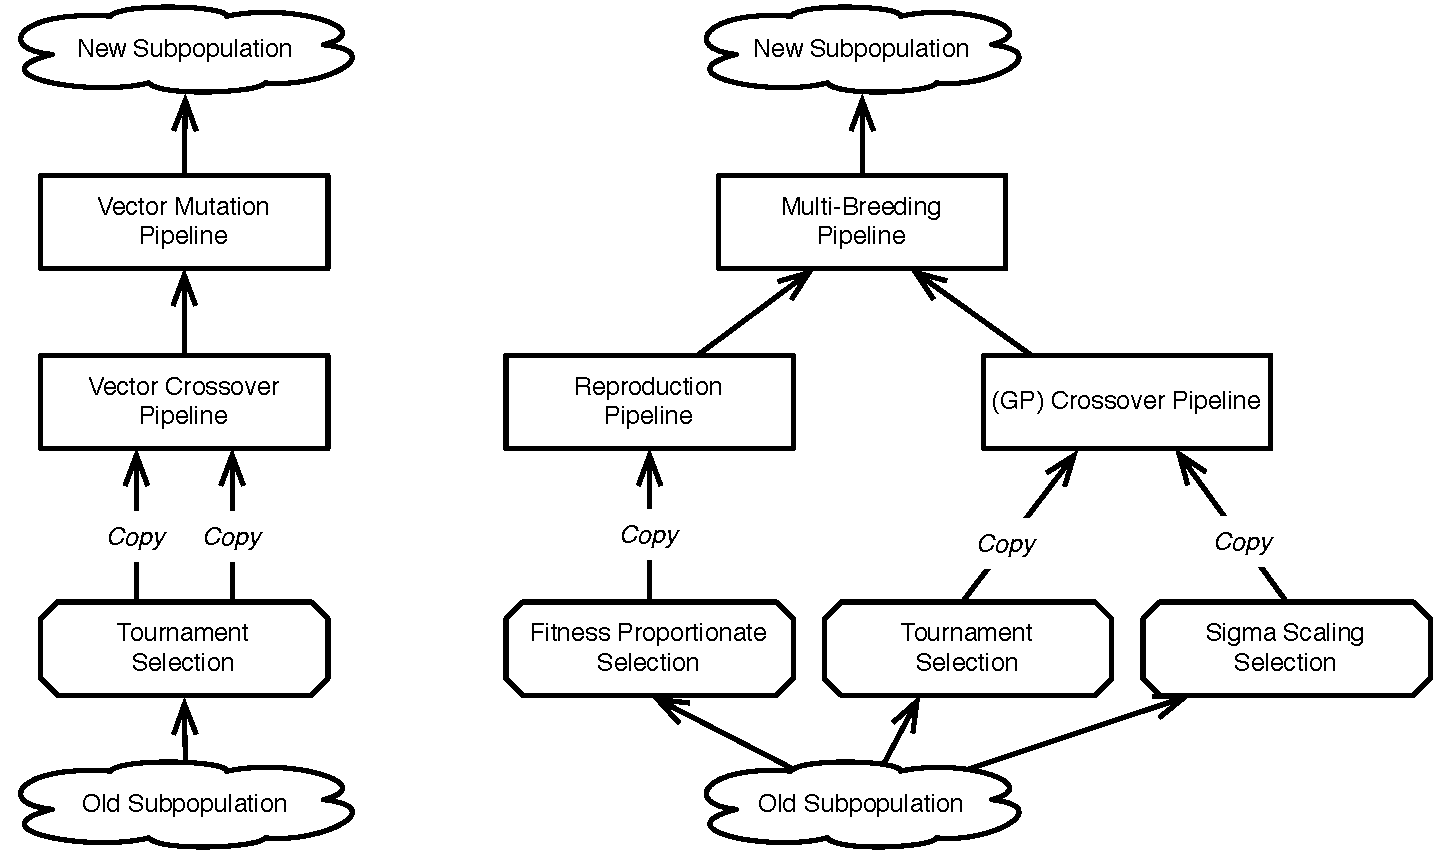
\includegraphics[height=3.8in]{BreedingPipelines.pdf}
\end{center}
\caption{Two example Breeding Pipelines.}
\label{BreedingPipelineDiagram}
\end{figure}





\subsection{Breeding Pipelines and BreedingSources}

A Breeding Pipeline is a chain of selection and breeding operators whose function is to draw from Individuals in an old Subpopulation to produce individuals in a new Subpopulation.

Breeding Pipelines consist of two kinds of objects.  First there are {\bf Selection Methods}, which select Individuals from the old Subpopulation and return them.  Then there are {\bf Breeding Pipelines} (what would have better been called \textit{\textbf{Breeding Operators}}), which take Individuals from Selection Methods or from other Breeding Pipelines, modify them in some way, and return them.

The Breeding Pipeline structure isn't actually a {\it pipeline}: it's really a tree (or in some situations, a directed acyclic graph).    The leaf nodes in the graph tree are the Selection Methods (subclasses of \class{ec.SelectionMethod}, and the nonleaf nodes are the Breeding Pipeline objects (subclasses of \class{ec.BreedingPipeline}). 

Each BreedingPipeline object can have some \(N\) {\bf sources} (children) from which it draws Individuals.  Both \class{ec.SelectionMethod} and \class{ec.BreedingPipeline} are subclasses of the abstract superclass \class{ec.BreedingSource}, and so can function as sources for BreedingPipelines.  SelectionMethods do not have sources: rather, they draw Individuals directly from the old Subpopulation.

BreedingSources (and BreedingPipeline, and SelectionMethods) are Prototypes, and so must implement the \method{clone()}, \method{defaultBase()}, and \method{setup(...)} methods.  BreedingSources also implement three special methods which perform the actual selection and breeding, which we describe here.  When a Breeder wishes to produce a series of new Individuals from an old Subpopulation, it begins by calling the method

\java{%
public abstract void prepareToProduce(EvolutionState state, int subpopulation,\\
\hsp{\fill}int thread);
}

This instructs the BreedingSource to prepare for a number of requests for Individuals drawn from subpopulation number \variable{subpopulation}.  During this method the BreedingSource will, at a minimum, call \method{prepareToProduce(...)} on each of its sources.

Next, the Breeder calls the following zero or more times to actually produce the Individuals:

\java{%
public abstract int produce(int min, int max, int start, int subpopulation,\\
\hsp{\fill}Individual[] inds, EvolutionState state, int thread);
}

This instructs the BreedingSource to produce between \variable{min} and \variable{max} Individuals drawn from subpopulation number \variable{subpopulation}.  The Individuals are to be placed in the \variable{inds} array at slots \variable{inds[start],~inds[start+1],~...}  Finally the method returns the actual number of Individuals produced.

Last, the Breeder calls the following method to give the BreedingSource an opportunity to clean up.  The BreedingSource in turn, at a minimum, will call the same method on each of its sources.

\java{%
public abstract void finishProducing(EvolutionState state, int subpopulation,\\
\hsp{\fill} int thread);
}

Additionally, BreedingSources implement three other methods.  The first:

\java{%
public abstract int typicalIndsProduced();
}

This method returns the number of individuals a BreedingSource would produce by default if not constrained by \variable{min} and \variable{max}.  The method can return any number \(> 0\).

The next method:

\java{%
public abstract boolean produces(EvolutionState state, Population newpop,\\
\hsp{\fill}int subpopulation, int thread);
}

\noindent ... returns \variable{true} if the BreedingSource believes it can validly produce Individuals of the type described by  the given Species, that is, by \variable{newpop.subpops[subpopulation].species}.  This is basically a sanity check.  At the minimum, the BreedingSource should call this method on each of its sources and return \variable{false} if any of them return \variable{false}.

Last, we have the hook...

\java{%
public void preparePipeline(Object hook);
}

You don't have to implement this at all.  ECJ does not call this method nor implement it in any of its BreedingSources beyond the default implementation (which in BreedingPipeline calls the method in turn on each of its sources).  This method simply exists in the case that you need a way to communicate with all the methods of a BreedingPipeline at some unusual time.



\subsection{SelectionMethods}
\label{selectionmethods}

Selection Methods by default implement the \method{typicalIndsProduced()} method to return \variable{SelectionMethod.INDS\_PRODUCED} (that is, 1).  

Furthermore, the default implementation of the \method{produces} method,

\java{%
public abstract boolean produces(EvolutionState state, Population newpop,\\
\hsp{\fill}int subpopulation, int thread);
}

\noindent ...just returns \variable{true}.  But you may wish to use this method to check to make sure that your SelectionMethod knows how to work with the kind of Fitnesses found in the given subpopulation, that is, \variable{state.population[subpopulation].f\_prototype}.

The default implementations of \method{prepareToProduce(...)} and \method{finishProducing(...)} do nothing at all; though some kinds of SelectionMethods, such as Fitness Proportionate Selection (\class{ec.select.FitProportionateSelection}), use \method{prepareToProduce(...)} to prepare probability distributions based on the Subpopulation in order to select properly.

SelectionMethods are sometimes called upon not to produce an Individual but to provide an {\it index} into a subpopulation where the Individual is located\,---\,perhaps to kill that Individual and place another Individual in its stead.  To this end, SelectionMethods have an alternative form of the \method{produce(...)} method:

\java{%
public abstract int produce(int subpopulation, EvolutionState state,\\
\hsp{\fill}int thread);
}

This method must return the index of the selected individual in the Subpopulation given by

\java{%
state.population.subpops[subpopulation].individuals;
}

\subsubsection{Implementing a Simple SelectionMethod}

Implementing a SelectionMethod can be as simple as overriding the ``alternative'' form of the \method{produce(...)} method.  You don't have to implement the ``stanard'' form of  \method{produce(...)} because its default implementation calls the alternative form and handles the rest of the work for you.

To select an individual at random from a Subpopulation, you could simply implement the ``alternative'' form to return a random number between 0 and the size of the subpopulation in question:

{\small\begin{verbatim}
public int produce(int subpopulation, EvolutionState state, int thread)
    {
    return state.random[thread.next(
            state.population.subpops[subpopulation].individuals.length)];
    }
\end{verbatim}}

You'll want to always implement the alternative form of \method{produce(...)}.  But in some cases you may wish to also reimplement the ``standard'' form of \method{produce(...)} for some special reason.\footnote{Many ECJ selection methods implement the ``standard'' form in addition to the ``alternative'' simply to be pedantic\,---\,it's very slightly faster\,---\,but that's not a good reason nowadays.}  It's a bit more involved but not too hard.  We start by determining how many individuals we'll produce, defaulting with 1:

{\small\begin{verbatim}
public int produce(int min, int max, int start, int subpopulation, Individual[] inds,
                   EvolutionState state, int thread)
    {
        int n = 1;
        if (n>max) n = max;
        if (n<min) n = min;
\end{verbatim}}

Next we select \(n\) individuals from the old subpopulation and place them into slots  \variable{inds[start] ... inds[start+n-1]}.  Here we're do it randomly:

{\small\begin{verbatim}
        for(int q = 0; q < n; q++)
            {
            Individual[] oldinds = state.population.subpops[subpopulation].individuals;
            inds[start+q] = oldinds[state.random[thread].nextInt(
                    state.population.subpops[subpopulation].individuals.length )];
            }
        return n;
        }
\end{verbatim}}


\subsubsection{Standard Classes}

There are a number of standard SelectionMethods available in ECJ, all found in the \package{ec.select} package.

\begin{itemize}
\item \class{ec.select.FirstSelection} always returns the first individual in the Subpopulation.  This is largely used for testing purposes.

\item \class{ec.select.RandomSelection} returns an Individual chosen uniformly at random.  Basically it does the same thing as the example given above.

\item \class{ec.select.FitProportionateSelection}\footnote{It's called FitProportionateSelection rather than FitnessProportionateSelection for a historical reason: MacOS 9 didn't allow filenames longer than 32 characters, and {\tt FitnessProportionateSelection.class} is 35 characters long.} uses {\bf Fitness-Proportionate Selection}, sometimes called {\bf Roulette Selection}, to pick individuals. Thus \class{ec.select.BestSelection} requires that all fitnesses be non-negative.

\item \class{ec.select.SUSSelection} selects individuals using {\bf Stochastic Universal Sampling}, a low-variance version of Fitness-Proportionate selection in which highly fit individuals are unlikely to {\it never} be chosen.  Every new generation, and \(M\) selection events thereafter, it shuffles the Subpopulation, then computes the next \(M\) individuals to be selected in the future.  ECJ assumes that \(M\) is the size of the Subpopulation.  Fitnesses must be non-negative.  You have the option of whether or not to shuffle the Subpopulation first:

\params{%
{\it base}.shuffle = true
}

The default value is false.

\item \class{ec.select.SigmaScalingSelection} (written by Jack Compton, a former undergraduate at GMU) is another low-variance version of Fitness-Proportionate Selection, in which modified versions of the Individuals' fitnesses are used to reduce the variance among them.  This is done by first computing the mean \(\mu\) and standard deviation \(\sigma\) among the fitnesses.  If \(\sigma=0\) no change is made.  Otherwise each modified fitness \(g\) is then treated as \(g \leftarrow 1 + \frac{f - \mu}{2 \sigma}\).  This can result in negative modified fitnesses, so we introduce a fitness floor: modified fitnesses are bounded to be no less than the floor.  Original fitnesses must be non-negative   To set this floor to 0.1 (a common value), you'd say:

\params{%
{\it base}.scaled-fitness-floor = 0.1
}

0.1 is the default value already, so this is redundant.

SigmaScalingSelection default base is \parameter{select.sigma-scaling}.


\item \class{ec.select.BestSelection} picks among the best or worst \(N\) individuals in the population, depending on a parameter.  The selection procedure among these \(N\) is fitness-proportionate selection.  Thus \class{ec.select.BestSelection} requires that all fitnesses be non-negative.  To make BestSelection pick among the best 5 Individuals, you could say:

\params{%
{\it base}.pick-worst = false\\
{\it base}.n = 5
}

The default value for \parameter{pick-worst} is false; and 1 for \parameter{n}.

BestSelection's default base is \parameter{select.best}.

\item \class{ec.select.BoltzmanSelection} (also written by Jack Compton) works like Fitness-Proportionate Selection, but uses modified fitness values according to a Boltzman (Simulated-Annealing-style) cooling schedule.  Initially BoltzmanSelection has a high {\it temperature} \(T\), and for each successive generation it decreases \(T\) by a {\it cooling rate} \(R\) as \(T \leftarrow T * R\).  Each modified fitness \(g\) is computed as \(g \leftarrow e^{f/T}\), where \(f\) is the original fitness.    Fitnesses must be non-negative.  When the temperature reaches 1.0, BoltzmanSelection reverts to FitnessProportionateSelection.  To set the initial temperature to 1000 and the cooling rate to 0.99, you'd say:

\params{%
{\it base}.starting-temperature = 1000\\
{\it base}.cooling-rate = 0.99
}

The default temperature is 1.0; and the default cooling rate is 0.0, which causes BoltzmanSelection to behave exactly like FitProportionateSelection.

BoltzmanSelection's default base is \parameter{select.boltzman}.

\item \class{ec.select.GreedyOverselection} is a variation of Fitness-Proportionate Selection which was common in the early genetic programming community (see Section~\ref{ec.gp}), but no longer.  The Individuals are sorted and divided into the ``fitter'' and ``less fit'' groups.  With a certain probability the ``fitter'' individuals will be selected (using Fitness-Proportionate Selection), else the ``less fit'' individuals will be selected (also using Fitness-Proportionate Selection).    Fitnesses must be non-negative.  To specify that the ``fitter'' group is 25\% of the Subpopulation, and that individuals are chosen from it 40\% of the time, you'd say:

\params{%
{\it base}.top = 0.25\\
{\it base}.gets = 0.40
}

GreedyOverselection's default base is \parameter{select.greedy}.

\item \class{ec.select.TournamentSelection} first chooses \(N\) individuals entirely at random with replacement (thus the same Individual may be chosen more than once).  Then from among those \(N\) it returns the fittest (or least fit, a parameter setting) Individual, breaking ties randomly.  \(N\) is often an integer but in fact it doesn't have to be: it can be any real-valued number \(N>0\).  If \(N\) isn't an integer, it's interpreted as follows: with probability \(N-\lfloor N\rfloor\) we choose \(\lceil N \rceil\) individuals at random, else we choose \(\lfloor N\rfloor\) individuals at random.    Fitnesses must be non-negative.  The most common setting for \(N\) is 2.  To use 2, and return the fittest individual rather than the least-fit one, say:

\params{%
{\it base}.size = 2\\
{\it base}.pick-worst = false
}

By default, \parameter{pick-worst} is false, so the second parameter is redundant here.

TournamentSelection's default base is \parameter{select.tournament}.

\item Finally, \class{ec.select.MultiSelection} is a special version of a SelectionMethod with \(N\) other SelectionMethods as sources.  Each time it must produce an individual, it picks one of these SelectionMethods at random (using certain probabilities) and has it produce the Individual instead.  To set up MultiSelection with two sources, TournamentSelection (chosen 60\% of the time) and FitnessProportionateSelection (chosen 40\% of the time), you'd say:

\params{%
{\it base}.num-selects = 2\\
{\it base}.select.0 = ec.select.TournamentSelection\\
{\it base}.select.0.prob = 0.60\\
{\it base}.select.1 = ec.select.FitnessProportionateSelection\\
{\it base}.select.1.prob = 0.40
}

MultiSelection's default base is \parameter{select.multiselect}.


\end{itemize}

\subsection{BreedingPipelines} BreedingPipelines (\class{ec.BreedingPipeline}) take Individuals from sources, typically modify them in some way, and hand them off.  Some BreedingPipelines are mutation or crossover operators; others are more mundane utility pipelines.  BreedingPipelines specify the required number of sources they use with the following method:

\java{%
public abstract int numSources();
}

This method must return a value \(>0\), or it can return the value \variable{BreedingPipeline.DYNAMIC\_SOURCES}, which indicates that the BreedingPipeline can vary its number of sources, and that the user must specify the number of sources with the parameter like this:

\params{%
{\it base}.num-sources = 3
}

You specify each source with a parameter.  For example, to stipulate sources 0, 1, and 2, you might say:

\params{%
{\it base}.source.0 = ec.select.TournamentSelection\\
{\it base}.source.1 = ec.select.TournamentSelection\\
{\it base}.source.2 = ec.select.GreedyOverselection
}

One trick available to you is to state that a source is the same source as a previous one using a special value called \parameter{same}.  For example, in the example above {\it two} TournamentSelection operators are created.  But if you said the following instead:

\params{%
{\it base}.source.0 = ec.select.TournamentSelection\\
{\it base}.source.1 = same\\
{\it base}.source.2 = ec.select.GreedyOverselection
}

\noindent ...then sources 0 and 1 will be the exact same object.  At any rate, the sources are then stored in the following instance variable:

\java{%
    public BreedingSource[] sources;
}


Unlike SelectionMethods, BreedingPipelines guarantee a {\bf copy-forward protocol}: any Individual produced by a BreedingPipeline will be unique to that thread.  The protocol is simple:  if a BreedingPipeline requests an Individual from a source, and that source is a SelectionMethod, the BreedingPipeline will copy the Individual and modify and hand off the copy.  But if the source is another BreedingPipeline, the BreedingPipeline will not copy the Individual but instead will just modify it directly and hand it off.  What's the point of this?  It enables multiple BreedingPipelines, one per thread, to be attached to an old Population and have {\it all} of them selecting Individuals out of that Population, modifying them, and generating new Individuals without the need for any locking.

Some BreedingPipelines, like crossover pipelines, have a very specific number of children they produce by default (the value returned by \method{typicalIndsProduced()}).  However many others (mutation operators, etc.) simply return whatever Individuals they receive from their sources.  For these, BreedingPipeline has a default implementation of \method{typicalIndsProduced()} which should work fine: it simply calls \method{typicalIndsProduced()} on all of its sources, and returns the minimum.   This computation is done via a simple utility function, \method{minChildProduction()}, one of two such methods which might be useful to you:

\java{%
    public int minChildProduction();\\
    public int maxChildProduction();
}

BreedingPipeline has default implementations of the \method{produces(...)}, \method{prepareToProduce(...)}, \method{finishProducing(...)}, and \method{preparePipeline(...)} methods, all of which call the same methods on the BreedingPipeline's children.

One final option common to most BreedingPipelines which make modifications (mutation, crossover): you can specify the probability that the pipeline will operate at all, or if Individuals will simply be passed through.  For example, let's say you're using a crossover pipeline of some sort, which creates two children from its sources, then crosses them over and returns them.  If you state:

\params{%
{\it base}.likelihood = 0.8
}

\noindent ...then with an 0.8 probability crossover will occur as normal.  But with a 0.2 probability two Individuals from the sources will be simply copied and returned, with no crossover occurring.



\subsubsection{Implementing a Simple BreedingPipeline}

To implement a BreedingPipeline, at a minimum, you'll need to override two methods: \method{numSources()} and \method{produce(...)}.  \method{numSources()} is easy.  Just return the number of sources your BreedingPipeline requires, or \variable{BreedingPipeline.DYNAMIC\_SOURCES} if the number can be any size specified by the user.  For example, to make a mutation pipeline, we probably want a single source, which we'll extract Individuals from and mutate:

{\small\begin{verbatim}
public int numSources() { return 1;}
\end{verbatim}}

Now we need to implement the \method{produce(...)} method.  Most mutation procedures ask their sources to produce some number of Individuals for them (however many the source prefers), and then mutate those Indviduals and return them.  We can ask our source to produce sources like this:

{\small\begin{verbatim}
public int produce(int min, int max, int start, int subpopulation, Individual[] inds,
                   EvolutionState state, int thread)
    {
    int n = sources[0].produce(min,max,start,subpopulation,inds,state,thread);
\end{verbatim}}

The source has taken the liberty of filling slots \variable{inds[start] ... inds[start+n-1]} with \(\text{\variable{min}} \geq \text{\variable{n}} \geq \text{\variable{max}}\) Individuals.  Next we need to decide whether to bother mutating at all, based on the \parameter{likelihood} parameter.  We'll use the following utility method to help us:

\begin{methods}{ec.BreedingPipeline}
\mthd{public int reproduce(int \textit{n}, int \textit{start}, int \textit{subpopulation}, Individual[] \textit{inds}, EvolutionState \textit{state}, int \textit{thread},}
\hsp{\fill}{\sf boolean \textit{produceChildrenFromSource})}\\
If {\it produceChildrenFromSource} is true, extracts \(n\) Individuals from Source 0 of the BreedingPipeline, and places them in locations \variable{inds[start] ... inds[start+n-1]}, else works with the existing Individuals in those slots. If Source 0 is a SelectionMethod, the individuals in \variable{inds[start] ... inds[start+n-1]} are replaced with clones. Then \(n\) is returned.
\end{methods}

We do a coin-flip to determine whether or not to use this method to just clone some individuals from the Source or to go ahead and mutate them.  If the former, since our Source has already produced the children, we call this method, passing in {\it false} for the last argument:

{\small\begin{verbatim}
    // should we bother mutating at all, or just reproduce?
    if (!state.random[thread].nextBoolean(likelihood))
        return reproduce(n, start, subpopulation, inds, state, thread, false); 
\end{verbatim}}

At this point we're committed to mutating the \(n\) Individuals.  First we need to clone them if Source 0 (our only Source) was a SelectionMethod, since it doesn't clone them for us:

{\small\begin{verbatim}
    // clone the individuals if necessary
    if (!(sources[0] instanceof BreedingPipeline))
        for(int q=start;q<n+start;q++)
            inds[q] = (Individual)(inds[q].clone());
\end{verbatim}}

Now we can mutate the Individuals.  How mutation occurs depends on the representation of the Individual of course, so we'll fake it with a comment:

{\small\begin{verbatim}
    for(int q=start;q<n+start;q++)
        {
        // modify inds[q] somehow
        }
    return n;
    }
\end{verbatim}}


\subsubsection{Standard Classes}

Most BreedingPipelines are custom for your representation: vectors and trees etc. all have their own special ways of being crossed over or mutated.  However there are some utility BreedingPipelines you should be aware of, all stored in the \package{ec.breed} package:

\begin{itemize}
\item \class{ec.breed.ReproductionPipeline} is by the most common utility BreedingPipeline.  In response to a request for \(N\) individuals, ReproductionPipeline requests the same number from its single source, then simply returns them (copying if necessary). ReproductionPipeline has one rarely-used parameter, which indicates if it {\it must} copy the indivdiuals even if it's not required to maintain the copy-forward protocol:

\params{%
{\it base}.must-clone = true
}

By default, \parameter{must-clone} is false.

\item Also common is \class{ec.breed.MultiBreedingPipeline}, which takes some \(M\) sources\,---\,determined by the user\,---\,and when asked to produce Individuals, chooses randomly among its sources to produce the Individuals for it.  It then returns those Individuals.   This is a common BreedingPipeline used in genetic programming (Section~\ref{ec.gp}).  Recall that to stipulate the number of sources, you say:

\params{%
{\it base}.num-sources = 2
}

Each source can be accompanied with a probability that this source will be chosen.  For example, to state that the first Source is a ReproductionPipeline, chosen 90\% of the time, and that the second is a Tournament Selection, chosen 10\% of the time, we'd say something like:

\params{%
{\it base}.source.0 = ec.select.TournamentSelection\\
{\it base}.source.0.prob = 0.90\\
{\it base}.source.1 = ec.breed.ReproductionPipeline\\
{\it base}.source.1.prob = 0.10
}

You can also state that the number of Individuals returned by any source must be exactly the same\,---\,specifically, the maximum that any one of them would return in response to a given request.  For example, if you had a Crossover pipeline (which normally returns 2 Indivdiuals) and a Reproduction pipeline (which normally returns 1 Individual), you could force both of them to return 2 Individuals if called on.  This is done by saying:

\params{%
{\it base}.generate-max = true
}

By default, \parameter{generate-max} is true, so this is redundant.

\item \class{ec.breed.BufferedBreedingPipeline} buffers up Individual requests and then hands them out one by one.  When you first call \method{produce()} on a BufferedBreedingPipeline, regardless of the number of Individuals requested, it will in turn demand some \(N\) children from its single source.  It then stores them in a buffer and hands them to this and later \method{produce()} requests until they are depleted, at which time it requests \(N\) more, and so on.  This value of \(N\) is set like this:

\params{%
{\it base}.num-inds = 10
}

Why would you want to do this? Primarily tricks like the following.  Let's say you want to create a crossover operator which produces two children, which are then fed into {\it another} different crossover operator and thus are crossed over {\it again}.  Ordinarily you'd think you could do it along these lines:

\params{%
pop.subpop.0.pipe.0 = ec.app.myCrossover\\
pop.subpop.0.pipe.0.source.0 = ec.app.myOtherCrossover\\
pop.subpop.0.pipe.0.source.1 = same
}

Looks good, right?  Not so fast.  The {myCrossover} class will request exactly one individual from each of its sources.  First it'll request from source 0, which will cross over two children, return one, {\it and throw away the other}.  Then it'll request from source 1, which will do exactly the same thing again even though it's the same object.  As a result you're not crossing over two individuals twice.  You're crossing over individuals which are the result of separate earlier crossovers.  But if you did it instead like this:

\params{%
pop.subpop.0.pipe.0 = ec.app.myCrossover\\
pop.subpop.0.pipe.0.source.0 = ec.select.BufferedBreedingPipeline\\
pop.subpop.0.pipe.0.source.1 = same\\
pop.subpop.0.pipe.0.source.0.num-inds = 2\\
pop.subpop.0.pipe.0.source.0.source.0 = ec.app.myOtherCrossover\\
pop.subpop.0.pipe.0.source.0.source.1 = same
}

Now {myCrossover} requests one child from {BufferedBreedingPipeline}, which in turn demands {\it two} children from {myOtherCrossover}, which crosses over two Individuals and returns them.  {BufferedBreedingPipeline} returns one of the Individuals.  Then {myOtherCrossover} requests the second child, and {BufferedBreedingPipeline} returns the other Individual out of its buffer.  Problem solved.

\item \class{ec.breed.ForceBreedingPipeline} takes a single source.  In response for a request for \(N\) individuals, ForceBreedingPipeline in turn requests up to some \(M\) Individuals from its source.  If \(M>N\), then ForceBreedingPipeline requests exactly \(N\) indivdiuals.  If \(M<N\), then ForceBreedingPipeline repeatedly requests \(M\) individuals to fill the \(N\), until possibly the last request, where it requests the remainder.  For example, if \(N=15\) and \(M=4\), then ForceBreedingPipeline will request 4, then 4, then 4, then 3 Individuals and return them all.

This trick is sort of the counterpart to BufferedBreedingPipeline: it gives you a way of demanding a certain number of individuals from a pipeline (like a CrossoverPipeline) which doesn't normally return that number.  It's only occasionally useful in practice though.

\item Last, \class{ec.breed.GenerationSwitchPipeline} takes two sources.  In response to a request for individuals, for generations 1 through \(N-1\) GenerationSwitchPipeline will request Indivduals from source 0.  For generations \(N\) and on,  GenerationSwitchPipeline will request Individuals from source 1.  You specify the switch-generation \(N\) as:

\params{%
{\it base}.switch-at = 15
}

Like ReproductionPipeline, GenerationSwitchPipeline can guarantee that both of its sources always return the same number of individuals (the maximum of the two) with:

\params{%
{\it base}.generate-max = true
}

By default, \parameter{generate-max} is true, so this example is redundant.



\end{itemize}

\begin{figure}[t]
\begin{center}
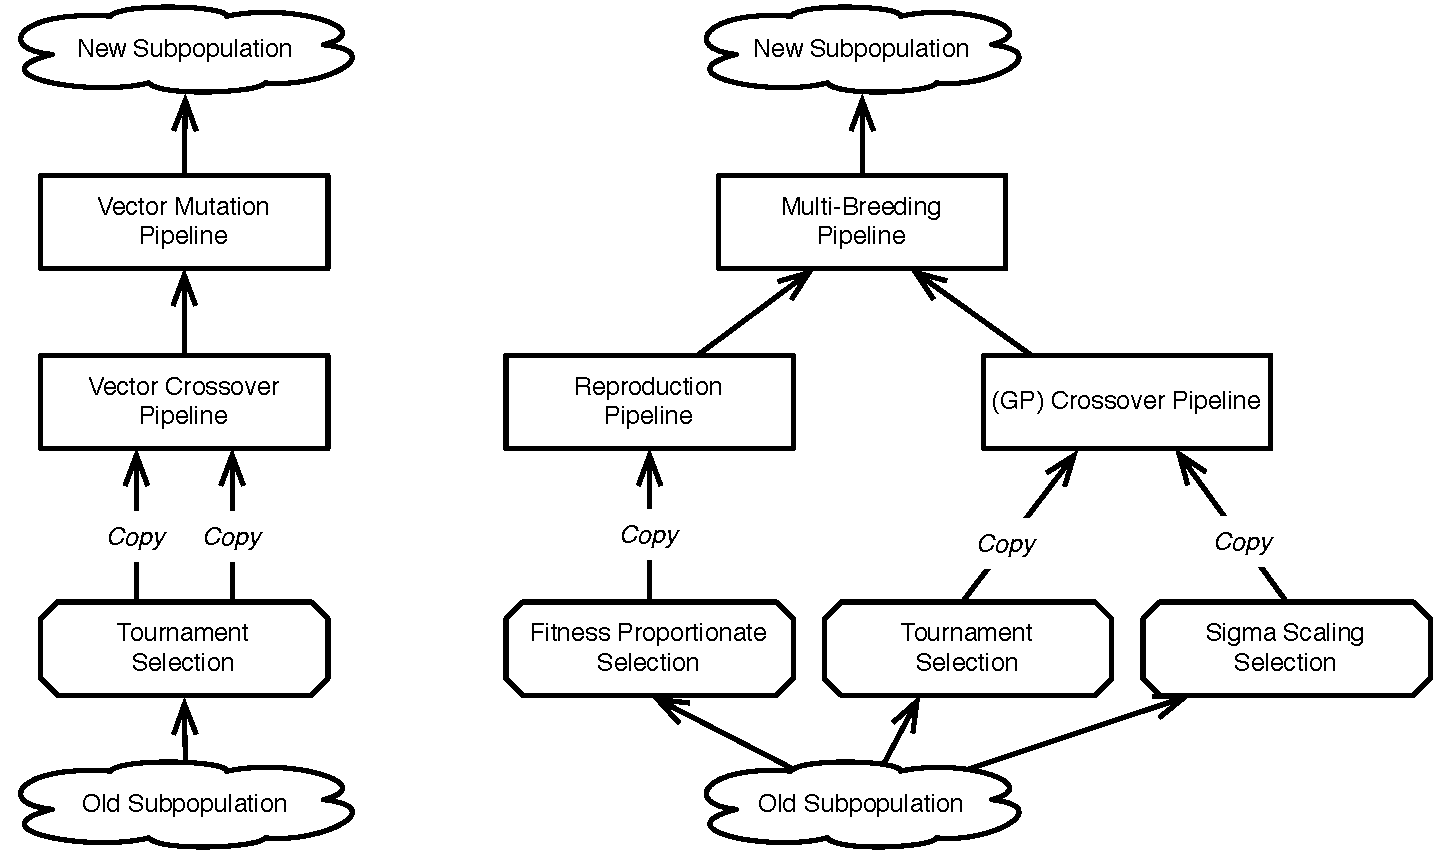
\includegraphics[height=3.8in]{BreedingPipelines.pdf}
\end{center}
\caption{Two example Breeding Pipelines (Repeat of Figure \ref{BreedingPipelineDiagram}).}
\label{BreedingPipelineDiagram2}
\end{figure}

\subsection{Setting up a Pipeline}
\label{SettingUpAPipeline}

Setting up a pipeline using parameters sometimes isn't entirely obvious.  Let's do the two examples shown in Figure \ref{BreedingPipelineDiagram2}, in both cases setting up a pipeline for Subpopulation 0.

\subsubsection{A Genetic Algorithm Pipeline}
The left figure is a Breeding Pipeline common to the Genetic Algorithm: two Individuals are selected from the old Subpopulation, then copied and crossed over, and the two children are then mutated and added to the new Subpopulation.  To build the pipeline, we work our way backwards: first defining the mutator as the top element, then the crossover as its source, then the selector as the crossover's two sources.

First the mutator.  We'll use \class{ec.vector.VectorMutationPipeline}, a common mutator for vector individuals.  Subpopulation 0's species holds the prototypical pipeline:

\params{%
pop.subpop.0.species.pipe = ec.vector.VectorMutationPipeline
}

Next we define its sole source: the crossover operator (\class{ec.vector.VectorCrossoverPipeline})

\params{%
pop.subpop.0.species.pipe.source.0 = ec.vector.VectorCrossoverPipeline
}

Back to building the Pipeline.  Crossover has two sources.  We'd like them to both be the Tournament Selector (they could be different Tournament Selectors; it doesn't really matter):

\params{%
pop.subpop.0.species.pipe.source.0.source.0 = ec.select.TournamentSelection\\
pop.subpop.0.species.pipe.source.0.source.1 = same
}

Tournament Selection has a tournament size operator.  Since we're using the same selector for both sources, we only need to set it once:

\params{%
pop.subpop.0.species.pipe.source.0.source.0.size = 2
}

We could also just set the default parameter for all tournament selectors:

\params{%
select.tournament.size = 2
}

Perhaps we'd like the second source to use a tournament size of 4.  To do this we'd need to use a separate selector, so we could do this:

\params{%
pop.subpop.0.species.pipe.source.0.source.1 = ec.select.TournamentSelection\\
pop.subpop.0.species.pipe.source.0.source.1.size = 4
}

This would also override the default we just set, so it'd work whether or not we used the default-setting approach for source 0.

VectorCrossoverPipeline and VectorMutationPipeline, discussed later, have various parameters; to simplify the pipeline-building procedure, the \class{ec.vector} package (Section~\ref{ec.vector}) puts these parameters in the Species, not the pipeline.  For completeness sakes, let's include some of them here:

\params{%
pop.subpop.0.species = ec.vector.FloatVectorSpecies\\
pop.subpop.0.species.crossover-type = one\\
pop.subpop.0.species.mutation-prob = 1.0\\
pop.subpop.0.species.mutation-type = gauss\\
pop.subpop.0.species.mutation-stdev = 0.01
}

\subsubsection{A Genetic Programming Pipeline}

The right figure is a typical Genetic Programming pipeline (see Section~\ref{ec.gp}).  We begin with the root:

\params{%
pop.subpop.0.species.pipe = ec.breed.MultiBreedingPipeline
}

As discussed earlier, MultiBreedingPipeline can take any number of sources, so we have to specify it (to 2 here).  We also need to state the sources and the probabilities for each source.  We'll do 10\% Reproduction for the first source and 90\% Genetic Programming Crossover for the second.  We won't require the two sources to produce the same number of individuals: 

\params{%
pop.subpop.0.species.pipe.num-sources = 2\\
pop.subpop.0.species.pipe.generate-max = false\\
pop.subpop.0.species.pipe.source.0 = ec.breed.ReproductionPipeline\\
pop.subpop.0.species.pipe.source.0.prob = 0.10\\
pop.subpop.0.species.pipe.source.1 = ec.gp.koza.CrossoverPipeline\\
pop.subpop.0.species.pipe.source.1.prob = 0.90
}

In Genetic Programming normally we'd use Tournament Selection for all selectors.  But we'll do various selectors as shown in the Figure.  First the Fitness Proportionate Selection source for the ReproductionPipeline:

\params{%
pop.subpop.0.species.pipe.source.0.source.0 = ec.select.FitProportionateSelection
}

Next TournamentSelection (tournament size 7) as Crossover's first source:

\params{%
pop.subpop.0.species.pipe.source.1.source.0 = ec.select.TournamentSelection\\
pop.subpop.0.species.pipe.source.1.source.0.size = 7
}

Last, Sigma Scaling Selection as Crossover's second source:

\params{%
pop.subpop.0.species.pipe.source.1.source.1 = ec.select.SigmaScalingSelection\\
pop.subpop.0.species.pipe.source.1.source.1.scaled-fitness-floor = 0.1
}

(The default setting for \parameter{pop.subpop.0.species.pipe.source.1.source.1.scaled-fitness-floor} is already \parameter{0.1}, so it doesn't really need to be set.)

\section{Exchangers}
\label{ec.Exchanger}

An Exchanger is a subclass of \class{ec.Exchanger}, and is called both before and after breeding.  Exchangers form the basis of {\bf Island Models} in ECJ and will be discussed in-depth in Section~\ref{ec.exchange}.

Besides \method{setup(...)}, Exchangers have three basic functions, called at different times in the evolutionary cycle:

\java{%
public abstract Population preBreedingExchangePopulation(EvolutionState state);\\
public abstract Population postBreedingExchangePopulation(\\
\hsp{\fill}EvolutionState state);\\
public abstract String runComplete(EvolutionState state);
}

The first method is called prior to breeding a population.  It's largely available for Island Models to ship off members of the Population to remote ECJ processes.  The second method is called immediately {\it after} breeding a Population, and enables Island Models to import members from remote ECJ processes, possibly displacing newly-bred individuals.  The third method is called after \method{preBreedingExchangePopulation(...)} to determine whether or not the Exchanger thinks ECJ should shut down its process because some {\it other} process has found the optimal individual.  To cause ECJ to shutdown, return a String with a shutdown message of some sort (which will get printed out); otherwise return null.

Unless you're doing Island Models, almost certainly you'll use a default Exchanger called \class{ec.simple.SimpleExchanger} which does nothing to the Population at all.  To wit:

\params{%
exch = ec.simple.SimpleExchanger
}



\section{Statistics}
\label{ec.Statistics}

ECJ provides a large number of {\bf statistics hooks}, places where ECJ will call arbitrary methods on a Statistics object throughout the process.  Statistics objects are subclasses of \class{ec.Statistics} and often follow one or more {\bf statistics forms} which provide alternate Statistics hooks.  For example, \class{ec.steadystate.SteadyStateStatisticsForm}, discussed later in Section~\ref{ec.steadystate}, stipulates hooks for Statistics in steady-state evolution. The Statistics class \class{ec.simple.SimpleStatistics} and has hooks for both regular generational evolution (defined in \class{ec.Statistics}) and SteadyStateStatisticsForm.  Another basic Statistics class, \class{ec.simple.SimpleShortStatistics}, has hooks only for generational evolution.  Other Statistics classes exist, such as those found in Genetic Programming (Section~\ref{ec.gp}).

You can have as many Statistics objects as you want, but one Statistics object (usually arbitrarily chosen) must be the {\bf statistics root}.  To define an \class{ec.simple.SimpleStatistics} as the root, you say:

\params{%
stat = ec.simple.SimpleStatistics
}

Statistics objects usually, but not always, have a {\bf file} which they log their statistics results out to.  It's common to stipulate that file as:

\params{%
stat.file = \$out.stat
}

This tells SimpleStatistics to write to a file called \file{out.stat}, located right where the user launched ECJ (for a reminder on the meaning of the ``\$'', see Section~\ref{kindsofparameters}).  If you are running with multiple jobs (Section~\ref{jobs}), ECJ will automatically append the prefix \file{"jobs.{\it n}."}  to this filename, where \(n\) is the job number.  Thus the statistics file for job number 5 will be \file{"jobs.5.out.stat"}.  If no file is provided, SimpleStatistics will simply print out to the screen.

If ECJ is restarted from a checkpoint, SimpleStatistics will append to existing files rather than overwriting them.   SimpleStatistics also has an option to compress the file using GZIP (and thus add a \file{".gz"} suffix at the very end, as in \file{"jobs.5.out.stat.gz"}.  Note that if this option is used, SimpleStatistics will simply overwrite the file if restarted from a checkpoint.  The parameter is:

\params{%
stat.gzip = true
}

For each generation, the SimpleStatistics object prints out the best Individual of the generation using the \method{printIndividualForHumans(...)} method.  For example, generation 0 might have:

\script{%
Generation: 0\\
Best Individual:\\
Subpopulation 0:\\
Evaluated: T\\
Fitness: -1503.8322\\
 2.4502202187677815 0.9879236448665667 0.7631586426217085 0.6854305126240172
 }
 
 At the end of the run, the SimpleStatistics object prints out the best Individual of the run:

\script{%
Best Individual of Run:\\
Subpopulation 0:\\
Evaluated: T\\
Fitness: -185.78166\\
 -1.0393115193403102 -2.006026366200021 -0.03642166362331428 -1.1196984643947918
}

If your Problem implements the \method{describe(...)} method, SimpleStatistics will also ask the best-of-run Individual to describe itself at the very end of the file.

So how do you add additional Statistics objects?  As children of the root, or of one another.  Any Statistics object can have some \(n\) children.  Children are called the same hooks as their parents are.  To add another Statistics object (say, \class{ec.simple.SimpleShortStatistics}, we might add a child to the root:

\params{%
stat.num-children = 1\\
stat.child.0 = ec.simple.SimpleShortStatistics\\
stat.child.0.file = \$out2.stat
}

Notice that the file has changed: you don't want both Statistics objects writing to the same file!  If we wanted to add a third Statistics object (say, another \class{ec.simple.SimpleShortStatistics}), we could do it this way:

\params{%
stat.num-children = 2\\
stat.child.0 = ec.simple.SimpleShortStatistics\\
stat.child.0.file = \$out2.stat\\
stat.child.1 = ec.simple.SimpleShortStatistics\\
stat.child.1.file = \$out3.stat
}

\noindent ...or we could do it this way:

\params{%
stat.num-children = 1\\
stat.child.0 = ec.simple.SimpleShortStatistics\\
stat.child.0.file = \$out2.stat\\
stat.child.0.num-children = 1\\
stat.child.0.child.0 = ec.simple.SimpleShortStatistics\\
stat.child.0.child.0.file = \$out3.stat
}

The point is, you can hang a Statistics object as a child of any other Statistics object.  Pick your poison.

SimpleShortStatistics writes out a different kind of statistics from SimpleStatistics  In its basic form, for each generation it writes out a line of the following values, each separated by a space.

\begin{enumerate}
\item The generation number
\item {\it Once for each subpopulation...}
\begin{enumerate}
	\item The mean fitness of the subpopulation for this generation
	\item The best fitness of the subpopulation for this generation
	\item The best fitness of the subpopulation so far in the run
\end{enumerate}
\end{enumerate}

For example, we might have values like this...

\script{%
0 -1851.9916400146485 -1559.68 -1559.68 \\
1 -1801.2400487060547 -1557.7627 -1557.7627 \\
2 -1758.2322434082032 -1513.4955 -1513.4955 \\
3 -1715.5276463623047 -1420.0074 -1420.0074 \\
4 -1675.379030883789 -1459.842 -1420.0074 \\
5 -1637.332774291992 -1426.798 -1420.0074 
}

SimpleShortStatistics has an option for including more statistics.  If we turned on the following parameter:

\params{%
stat.child.0.gather-full = true
}

...we'd have the following values printed out:

\begin{enumerate}
\item The generation number
\item How long initialization took in milliseconds (for generation 0), or how long the previous generation took to breed to form this generation (for generations \(>0\)).
\item How many bytes initialization took (for generation 0), or how many bytes the previous generation took to breed to form this generation (for generations \(>0\)).  This is an approximation and in some cases might even be negative due to garbage collection.
\item How long evaluation took in milliseconds for this generation.
\item How many bytes evaluation took for this generation.    This is an approximation and in some cases might even be negative due to garbage collection.
\item {\it Once for each subpopulation...}
\begin{enumerate}
	\item The average size of an individual this generation (calling Indivdidual's \method{size()} method).
	\item The average size of an individual so far in the run.
	\item The mean fitness of the subpopulation for this generation
	\item The best fitness of the subpopulation for this generation
	\item The best fitness of the subpopulation so far in the run
	\item The size of the best individual this generation.
	\item The size of the best individual so far in the run.
\end{enumerate}
\end{enumerate}

For example, it might look like this:

\script{%
0 58 619752 11 0 100.0 100.0 -1851.16737622 -1536.3141 -1536.3141 100.0 100.0 \\
1 69 858032 13 8528 100.0 100.0 -1797.0600598 -1517.8112 -1517.8112 100.0 100.0 \\
2 50 852264 10 0 100.0 100.0 -1747.270633307 -1460.2653 -1460.2653 100.0 100.0 \\
3 56 -904648 9 6600 100.0 100.0 -1703.4300143 -1423.7004 -1423.7004 100.0 100.0 \\
4 50 861328 9 0 100.0 100.0 -1659.892714477 -1464.9053 -1423.7004 100.0 100.0 \\
5 59 -836488 9 0 100.0 100.0 -1619.276935424 -1347.0051 -1347.0051 100.0 100.0
}

\subsection{Implementing a Statistics Object}

A basic Statistics object implements one or more of the following hooks:

\java{%
    public void preInitializationStatistics(EvolutionState state); \\
    public void postInitializationStatistics(EvolutionState state);{~}// Generational\\
    public void preCheckpointStatistics(EvolutionState state); \\
    public void postCheckpointStatistics(EvolutionState state);\\
    public void preEvaluationStatistics(EvolutionState state);{~}{~}{~}{~}{~}{~}// Generational\\
    public void postEvaluationStatistics(EvolutionState state);{~}{~}{~}{~}{~}// Generational\\
    public void prePreBreedingExchangeStatistics(EvolutionState state);\\
    public void postPreBreedingExchangeStatistics(EvolutionState state);\\
    public void preBreedingStatistics(EvolutionState state);{~}{~}{~}{~}{~}{~}{~}{~}// Generational\\
    public void postBreedingStatistics(EvolutionState state);{~}{~}{~}{~}{~}{~}{~}// Generational\\
    public void prePostBreedingExchangeStatistics(EvolutionState state);\\
    public void postPostBreedingExchangeStatistics(EvolutionState state);\\
    public void finalStatistics(EvolutionState state, int result);
}

When these statistics hooks are called should be self-explanatory from the method name.  Note that the methods marked \variable{Generational} are only called by generational EvolutionState objects\,---\,notably the \class{ec.simple.SimpleEvolutionState} object.  There are also some additional hooks called by the \class{ec.steadystate} package for steady-state evolution (see Section~\ref{ec.steadystate}).

The \method{finalStatistics(...)} method, called at the end of an evolutionary run, contains one additional argument, \variable{result}.  This argument will be either \variable{ec.EvolutionState.R\_SUCCESS} or
\variable{ec.EvolutionState.R\_FAILURE}.  Success simply means that the optimal individual was discovered, and nothing more.

Whenever you override one of these methods, make certain to call \method{super(...)} first.  Let's say that we'd like to know what the size is of the very first individual created after initialization.  We might create a Statistics subclass which overrides this to print this size out to the screen:

\vbox{
\small\begin{verbatim}
public void postInitializationStatistics(EvolutionState state)
    {
    super.postInitializationStatistics(state);  // always call this
    state.output.println(state.population.subpops[0].individuals[0].size(), 0);  // stdout
    }
\end{verbatim}
}

We could also write to a file, but to do so we'd need to determine the file name.  We could do it in a manner similar to SimpleStatistics (ignoring the compression):
 
\vbox{
\small\begin{verbatim}
public static final String P_STATISTICS_FILE = "file";
public int log = 0;   // 0 by default means stdout

public void setup(final EvolutionState state, final Parameter base)
    {
    super.setup(state, base);
    File statisticsFile = state.parameters.getFile(base.push(P_STATISTICS_FILE),null);
    if (statisticsFile!=null) try
        {
        log = state.output.addLog(statisticsFile, true, false, null, false);
        }
    catch (IOException i)
        {
        state.output.fatal("An IOException occurred trying to create the log "
                + statisticsFile + ":\n" + i);
        }
    // else we'll just keep the log at 0, which is stdout
    }
\end{verbatim}
}

Now we can write out to the log:

\vbox{
\small\begin{verbatim}
public void postInitializationStatistics(EvolutionState state)
    {
    super.postInitializationStatistics(state);  // always call this
    state.output.println(state.population.subpops[0].individuals[0].size(), log);
    }
\end{verbatim}
}


\section{Debugging an Evolutionary Process}

A hint.  One helpful way to debug ECJ is via BeanShell (http://www.beanshell.org).  This tool is essentially a command-line for Java.  Using it, we can create an ECJ process and get it going quite easily.  Let's say that the parameter file is called "foo.params". We can type the following into BeanShell:

\vbox{
\small\begin{verbatim}
        show();
        import ec.*;
        args = new String[] { "-file", "foo.params" };
        database = Evolve.loadParameterDatabase(args);
        state = Evolve.initialize(database, 0);
        state.run(EvolutionState.C_STARTED_FRESH);
        Evolve.cleanup(state);
\end{verbatim}
}

This is basically a variation of the \method{main} code found in Section \ref{jobs}.  When \method{state.run(...)} is executed, ECJ will go through the entire evolutionary run.  It turns out that \method{state.run(...)} is really just a cover for three methods (at least, if we're starting from scratch rather than from a checkpoint).  They are: first calling \method{state.startFresh()}, then repeatedly calling \method{state.evolve()}, and when it returns something other than \variable{state.R\_NOTDONE}, finally calling \variable{state.finish(...)}, passing in what was returned.  In other words:

\vbox{
\small\begin{verbatim}
        show();
        import ec.*;
        args = new String[] { "-file", "foo.params" };
        database = Evolve.loadParameterDatabase(args);
        state = Evolve.initialize(database, 0);
        state.startFresh();
        result = EvolutionState.R_NOTDONE;
        while( result == EvolutionState.R_NOTDONE )
                {
                result = state.evolve();
                }
        state.finish(result);
        Evolve.cleanup(state);
\end{verbatim}
}

So how can we use this for debugging?  Well, BeanShell gives us full access to Java.  Let's try it on the \file{ecsuite.params} file.  We begin with the preliminaries:

\vbox{
\small\begin{verbatim}
        show();
        args = new String[] { "-file", "ecsuite.params" };
\end{verbatim}
}

BeanShell responds with:

\vbox{
\small\begin{verbatim}
<[Ljava.lang.String;@39617189>
\end{verbatim}
}

This is the String array.  We continue with:

\vbox{
\small\begin{verbatim}
        database = Evolve.loadParameterDatabase(args);
\end{verbatim}
}

BeanShell responds with the ParameterDatabase:

\vbox{
\small\begin{verbatim}
<{} : ({} : ({eval=ec.simple.SimpleEvaluator, pop.subpop.0=ec.Subpopulation, 
quit-on-run-complete=true, generations=1000, 
pop.subpop.0.species.pipe.source.0=ec.vector.breed.VectorCrossoverPipeline, 
pop.subpop.0.species.min-gene=-5.12, eval.problem=ec.app.ecsuite.ECSuite, 
state=ec.simple.SimpleEvolutionState, pop.subpop.0.species.mutation-type=gauss, 
pop=ec.Population, pop.subpop.0.duplicate-retries=2, select.tournament.size=2,
pop.subpops=1, pop.subpop.0.species.mutation-stdev=0.01, 
pop.subpop.0.species.pipe=ec.vector.breed.VectorMutationPipeline, 
pop.subpop.0.species.max-gene=5.12, pop.subpop.0.species.pipe.source.0.source.1=same, 
pop.subpop.0.species.pipe.source.0.source.0=ec.select.TournamentSelection, 
pop.subpop.0.species=ec.vector.FloatVectorSpecies, breed=ec.simple.SimpleBreeder, 
pop.subpop.0.species.mutation-prob=1.0, pop.subpop.0.species.genome-size=100, 
pop.subpop.0.species.crossover-type=one, finish=ec.simple.SimpleFinisher, 
parent.0=../../ec.params, init=ec.simple.SimpleInitializer, 
pop.subpop.0.species.ind=ec.vector.DoubleVectorIndividual, 
pop.subpop.0.species.fitness=ec.simple.SimpleFitness, pop.subpop.0.size=1000, 
eval.problem.type=rastrigin, stat=ec.simple.SimpleStatistics, 
exch=ec.simple.SimpleExchanger, stat.file=$out.stat} : ({checkpoint-modulo=1, 
evalthreads=1, checkpoint=false, breedthreads=1, prefix=ec, seed.0=time})))>
\end{verbatim}
}

Now we initialize the EvolutionState from the database:

\vbox{
\small\begin{verbatim}
        state = Evolve.initialize(database, 0);
\end{verbatim}
}

This causes ECJ to start printing to the screen something along these lines:


\vbox{
\small\begin{verbatim}
| ECJ
| An evolutionary computation system (version 19)
| By Sean Luke
| Contributors: L. Panait, G. Balan, S. Paus, Z. Skolicki, R. Kicinger, E. Popovici,
|               K. Sullivan, J. Harrison, J. Bassett, R. Hubley, A. Desai, A. Chircop,
|               J. Compton, W. Haddon, S. Donnelly, B. Jamil, and J. O'Beirne
| URL: http://cs.gmu.edu/~eclab/projects/ecj/
| Mail: ecj-help@cs.gmu.edu
|       (better: join ECJ-INTEREST at URL above)
| Date: July 10, 2009
| Current Java: 1.6.0_20 / Java HotSpot(TM) 64-Bit Server VM-16.3-b01-279
| Required Minimum Java: 1.4


Threads:  breed/1 eval/1
Seed: 1853290822 
<ec.simple.SimpleEvolutionState@1f5b0afd>
\end{verbatim}
}

Notice the last line\,---\,BeanShell is returning the EvolutionState.  Now we fire up the EvolutionState to initialize the first population:

\vbox{
\small\begin{verbatim}
        state.startFresh();
\end{verbatim}
}

... and get back:

\vbox{
\small\begin{verbatim}
Setting up
Initializing Generation 0
\end{verbatim}
}

The first population has been created.  Let's look at the first Individual:

\vbox{
\small\begin{verbatim}
        state.population.subpops[0].individuals[0]
\end{verbatim}
}

This produces:

\vbox{
\small\begin{verbatim}
<ec.vector.DoubleVectorIndividual@87740549{699618236}>
\end{verbatim}
}

Not very helpful.  Instead, let's have it printed:

\vbox{
\small\begin{verbatim}
        state.population.subpops[0].individuals[0].printIndividualForHumans(state, 0);
\end{verbatim}
}

This produces something more useful:

\vbox{
\small\begin{verbatim}
Evaluated: F
Fitness: 0.0
-4.3846934361930945 4.051323475292111 2.750742781209575 -2.1599970035296088 
3.5139838195638236 -4.326431483145531 -1.5799722524229094 -4.64489169381555 
-4.809825694271426 -0.6969239813124668 -4.322411553562226 4.8723307904232565 
2.8978088843319947 -4.311437772193992 -1.556903048013028 2.876699531303326 
-1.5461627480422133 -3.406470106152458 0.3510231690045371 -1.26870148662141 
-2.9943682283832675 -1.1321325429409796 -4.780798908878881 -2.789054768098288 
2.7957975471728034 -2.4529277934521363 0.06864524959557006 -2.807030901927618
-3.817734647565329 3.0018199187738803 3.893346256074625  -4.1700250768556355
-3.3035366716916714 -1.5300889532287534 -1.2924365390313826 2.6878356877535623
4.344108056131552 1.0732802812225044 1.804809997034555 0.6627493849916508 
1.6556742582736854 -3.8324177646471913 0.2901815515514814 -0.5045301890375606 
-2.755111883054377 -4.057309896490254 -2.097059222061862 -2.062611078568839 
3.676980437590175 3.4010063830636517 5.001876654997903 2.3637174851440808 
-2.3242430228722846 -0.2027490501614988 4.948796285958214 3.645393286308912 
-0.9981883696957627 -2.4911201811073296 2.281601570422807 -3.0028177298996583 
-0.6949487749058276 2.4115725052273005 2.2705630820859133 3.8198793397976756 
3.927188087275849 3.5439728479577974 4.195897069928313 4.064291914283307 
-1.6071055662352376 -0.45138576561254506 0.5382601925283925 2.2824947546503687 
-0.0837300863613164 -2.4997930740673895 0.06696037058102089 1.782243737261787 
-3.390249634178219 4.669336185081783 2.371290190775591 1.8743739255868377 
0.13349732700681827 2.808175830805574 -4.2297879656940705 -0.5781599273148448 
3.4174595199606577 2.5509508748123793 0.9574470878471297 1.181916131827328 
3.3128918249657184 3.5085201808925843 -0.8921840350705308 -4.016933626993176 
2.5591127486976983 1.580181276449899 -0.6102226049991097 1.0644092417475743 
0.5897983455130262 2.5504671849586904 -2.230897886457403 1.8133759722806326
\end{verbatim}
}

Now we're getting somewhere.  You could print out all the individuals like this:

\vbox{
\small\begin{verbatim}
        for(int i = 0; i < state.population.subpops[0].individuals.length; i++ )
                state.population.subpops[0].individuals[i].printIndividualForHumans(state, 0);
\end{verbatim}
}

... but I won't torture you with what comes out.  Instead, notice that the Individual has not been evaluated yet\,---\,just initialized with the Population.  We go through one evolutionary loop\,---\,evaluating the individuals and breeding a new Population\,---\,by calling 

\vbox{
\small\begin{verbatim}
        state.evolve();
\end{verbatim}
}

This produces:

\vbox{
\small\begin{verbatim}
Subpop 0 best fitness of generation: Fitness: -1493.534
<2>
\end{verbatim}
}

The first line was printed to the screen.  The second line indicates what \method{state.evolve()} returned.  2 is the value of \variable{EvolutionState.R\_NOTDONE}, indicating that the process needs to be evolved more.

Let's look at that first individual again:

\vbox{
\small\begin{verbatim}
        state.population.subpops[0].individuals[0].printIndividualForHumans(state, 0);
\end{verbatim}
}

...yielding...

\vbox{
\small\begin{verbatim}
Evaluated: F
Fitness: -1806.1432
-1.5595820609909528 -2.9941135630034292 -3.188550961391961 0.8673223056511647 
2.4308132097811472 -3.6298006589453533 -4.62193495641744 1.7381186900517611 
-3.2707539202577953 -2.8517369832386144 -4.701099579700639 1.1683479248633841 
0.10118833856168477 2.7982137159130787 -1.3673458253800685 -4.548719487000453 
-1.7852252742508177 -1.662999422245311 -4.891889992368657 2.0689413066938824 
4.64815452362056 4.03620579726471 -2.6065781548997413 2.8384398494616585 
-1.6231723965539844 -0.19641152832494305 -0.8025430015631594 -4.337733534634894 
-4.259188069209607 0.0974585410674078 4.878006291864429 4.187577755641656 
3.9507153065207605 -3.3456633008586922 3.7163666200189596 -0.7581028665673978 
4.28299933455259 1.8522464455693997 4.4324032846812935 -1.3209545115697914 
4.239911043319335 -2.7741200087506352 -3.181419981396656 -0.4574562816089688
3.9209870275697982 0.31049605413333237 -0.46868091240064014 -4.570530964131764 
-0.9126484738704782 3.6348709305820153 -1.800821491837854 -0.8548399118205554
-1.6874962921883667 2.628667604603462 0.060377157894385663 3.194354857448187
1.2106237734207714 -3.477534436566739 1.919326547065771 -3.74880517912247 
4.076653684533312  -2.9153006121227034 -2.4460232838375973 0.6128610868842217 
0.7785108819209824  -1.213371979065718 3.2441049504290587 -1.352037820951835 
1.151316091162472 0.3915293759690397 -0.15229424767569708 1.8192706794904545 
-3.057866603248519 -3.2217378304635926 3.7963181147558447 1.9609441782591566 
2.1365399986514815 -0.7608502832241196 -1.2202190662246202 -3.2592371482282956 
-2.612971504172355 3.1496849987738167 -5.083084415090031 -4.243405086300351 
3.8516939433487387 -4.87008846122508 1.012854792831603 3.77728764346906 
2.843506550933032 4.705462097924235 1.4291349248648448 3.8398215224809875 
1.1776568359195472 -4.784524531392207 2.765230136436807 -2.6521295800350555 
-2.271480494878218 -2.018481022639772 -2.2536397207045686 -1.5048357519436404
\end{verbatim}
}

It's a different Individual: the next generation one to be exact.  Notice that although it has a ``fitness'', in fact it's not been evaluated: the ``fitness'' is just nonsense cloned from a previous Individual.

So how do you see a population with fitness-evaluated Individuals?  Generational ECJ EvolutionState processes assess the fitness of a Population, then create a new Population and throw away the old one.  You can hold onto the old Population pretty easily.  Just do this:

\vbox{
\small\begin{verbatim}
        p = state.population;
        state.evolve();
\end{verbatim}
}

Now \variable{p} holds the old Population, filled with now-evaluated Individuals, and \variable{state.population} holds the next-generation Population, which hasn't been evaluated yet.  For example, if you say:

\vbox{
\small\begin{verbatim}
        p.subpops[0].individuals[0].printIndividualForHumans(state, 0);
\end{verbatim}
}

... you will get back something like this:

\vbox{
\small\begin{verbatim}
Evaluated: T
Fitness: -1779.4391
-1.5595820609909528 -2.9941135630034292 -3.188550961391961 0.8673223056511647 
2.4308132097811472 -3.6298006589453533 -4.62193495641744 1.7381186900517611 
-3.2707539202577953 -2.8517369832386144 -4.701099579700639 1.1683479248633841 
0.10118833856168477 2.7982137159130787 -1.3673458253800685 -4.548719487000453 
-1.7852252742508177 -1.662999422245311 -4.891889992368657 2.0689413066938824 
4.64815452362056 4.03620579726471 -2.6065781548997413 2.8384398494616585 
-1.6231723965539844 -0.19641152832494305 -0.8025430015631594 -4.337733534634894 
-4.259188069209607 0.0974585410674078 4.878006291864429 4.187577755641656
3.9507153065207605 -3.3456633008586922 3.7163666200189596 -0.7581028665673978 
4.28299933455259 1.8522464455693997 4.4324032846812935 -1.3209545115697914 
4.239911043319335 -2.7741200087506352 -3.181419981396656 -0.4574562816089688 
3.9209870275697982 0.31049605413333237 -0.46868091240064014 -4.570530964131764 
-0.9126484738704782 3.6348709305820153 -1.800821491837854 -0.8548399118205554 
-1.6874962921883667 2.628667604603462 0.060377157894385663 3.194354857448187 
1.2106237734207714 -3.477534436566739 1.919326547065771 -3.74880517912247 
4.076653684533312 -2.9153006121227034 -2.4460232838375973 0.6128610868842217 
0.7785108819209824 -1.213371979065718 3.2441049504290587 -1.352037820951835 
1.151316091162472 0.3915293759690397 -0.15229424767569708 1.8192706794904545 
-3.057866603248519 -3.2217378304635926 3.7963181147558447 1.9609441782591566 
2.1365399986514815 -0.7608502832241196 -1.2202190662246202 -3.2592371482282956 
-2.612971504172355 3.1496849987738167 -5.083084415090031 -4.243405086300351 
3.8516939433487387 -4.87008846122508 1.012854792831603 3.77728764346906 
2.843506550933032 4.705462097924235 1.4291349248648448 3.8398215224809875 
1.1776568359195472 -4.784524531392207 2.765230136436807 -2.6521295800350555 
-2.271480494878218 -2.018481022639772 -2.2536397207045686 -1.5048357519436404
\end{verbatim}
}

Notice that this Individual has been evaluated.  Its Fitness is valid.

\chapter{Basic Evolutionary Processes}

\begin{figure}[t]
\begin{center}
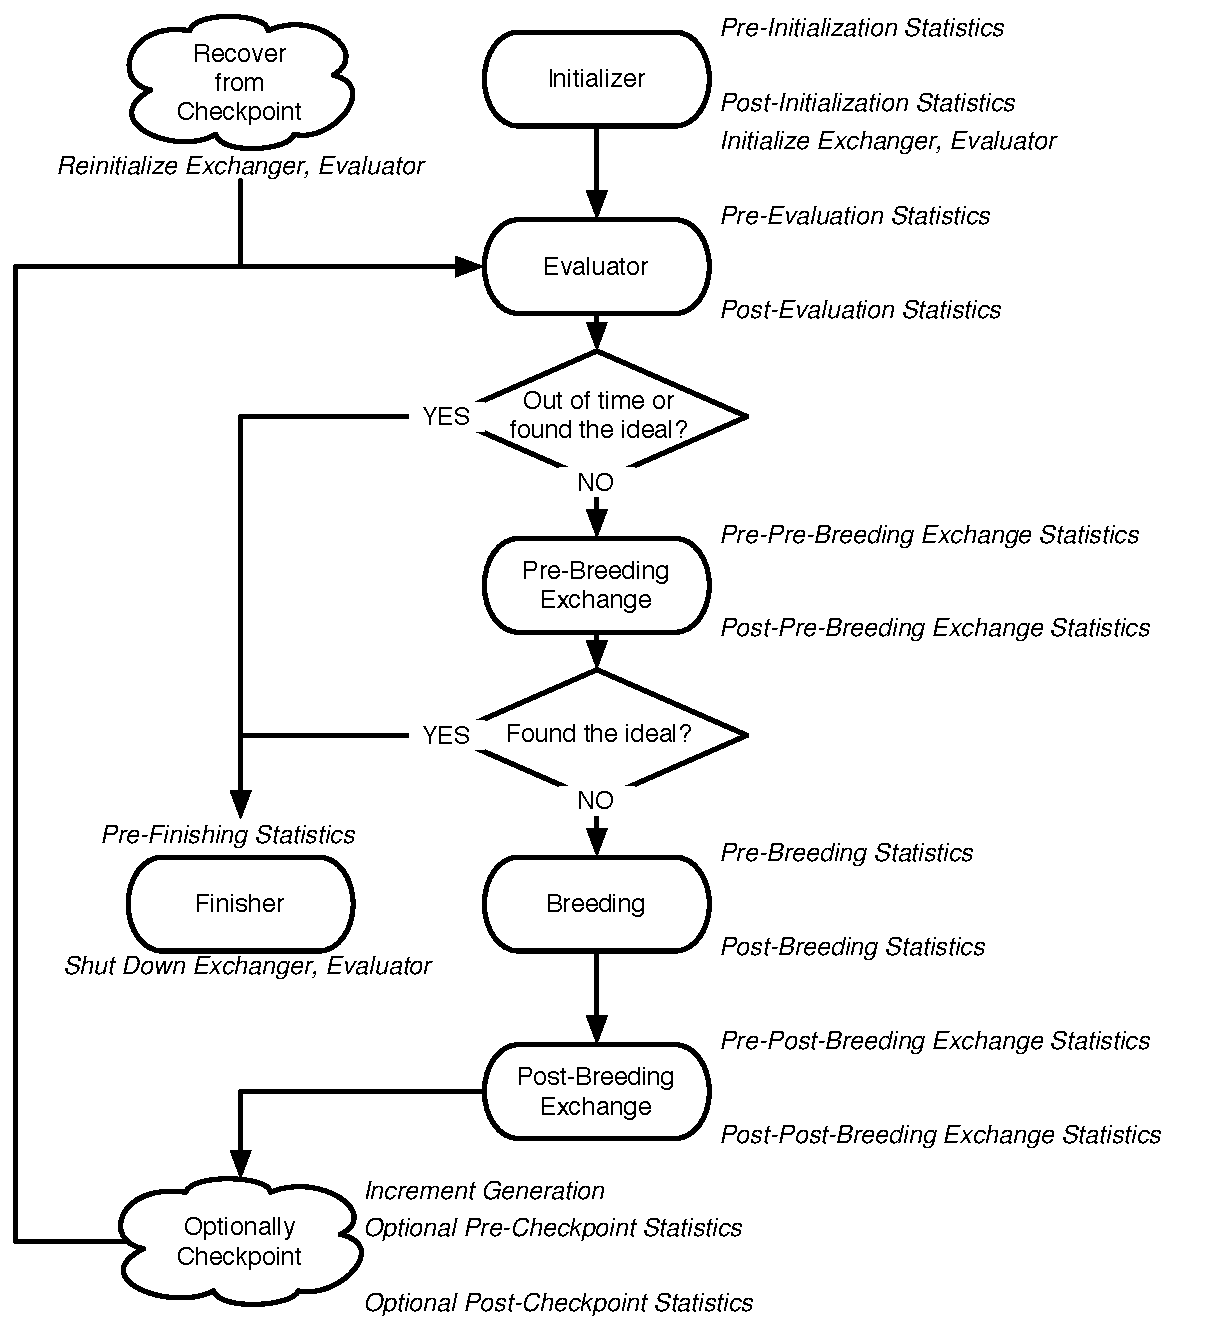
\includegraphics[height=6.3in]{EvolutionState.pdf}
\end{center}
\caption{Top-Level Loop of ECJ's \class{SimpleEvolutionState} class, used for basic generational EC algorithms.  Various sub-operations are shown occurring before or after the primary operations.  The full population is revised each iteration. A repeat of Figure \ref{EvolutionState}.}
\label{EvolutionState2}
\end{figure}
\afterpage{\clearpage}

\section{Generational Evolution}

ECJ is most commonly used for generational evolution: where a whole Population is evaluated, then updated, at a time.  There are a number of packages which use generational evolution, but the two most common are the \package{ec.simple} package, which does Genetic Algorithm style generational evolution, and the \package{ec.es} package which does Evolution Strategies.

\subsection{The Genetic Algorithm (The \package{ec.simple} Package)}
\label{ec.simple}

We've pretty much covered everything in the \package{ec.simple} package throughout Section~\ref{ec.EvolutionState}.  But just a quick reminder:

\begin{itemize}
\item \class{ec.simple.SimpleEvolutionState} subclasses \class{ec.EvolutionState} to provide the generational top-level loop shown in Figure \ref{EvolutionState2}.  Each generation the entire Population is handed to the Evaluator, then the Breeder.  The class adds no new parameters beyond those defined in EvolutionState. 
\item \class{ec.simple.SimpleBreeder} subclasses \class{ec.Breeder} to provide multithreaded breeding and elitism.  SimpleBreeder was discussed at length in Section~\ref{breeders}.
\item \class{ec.simple.SimpleEvaluator} subclasses \class{ec.Evaluator} to provide multithreaded evaluation.  SimpleEvaluator adds no new parameters beyond those defined in Evaluator, and was discussed at length in Section~\ref{ec.Evaluator}.
\item \class{ec.simple.SimpleFitness} subclasses \class{ec.Fitness} to provide a simple fitness consisting of a single floating-point number, where higher fitness values are preferred.  SimpleFitness also holds a boolean flag indicating whether the fitness assigned is the optimal fitness.  SimpleFitness adds no new parameters beyond those defined in Fitness, and was discussed at length in Section~\ref{ec.Fitness}.
\item \class{ec.simple.SimpleProblemForm} defines the kind of methods which must be implemented by Problems used by a SimpleEvaluator, and was discussed at length in Section~\ref{ec.Problem}.  As a reminder, the two methods defined by SimpleProblemForm are \method{evaluate(...)}, which evaluates an individual and sets its fitness; and \method{describe(...)}, which evaluates an individual solely for the purpose of writing a detailed description about the individual's performance out to a stream. They look like this:

\java{%
public void evaluate(EvolutionState state, Individual ind,\\
\hsp{\fill}int subpopulation, int threadnum);\\
public void describe(EvolutionState state, Individual ind,\\
\hsp{\fill}int subpopulation, int threadnum, int log);
}

\item \class{ec.simple.SimpleInitializer} subclasses \class{ec.Initializer} to provide multithreaded breeding and elitism.  SimpleInitializer adds no new parameters beyond those defined in Initializer, and was discussed at length in Section~\ref{ec.Initializer}.
\item \class{ec.simple.SimpleFinisher} subclasses \class{ec.Finisher} and does nothing at all.  SimpleFinisher was discussed at length (so to speak) in Section~\ref{ec.Finisher}.
\item \class{ec.simple.SimpleExchanger} subclasses \class{ec.Exchanger} and does nothing at all.  SimpleExchanger was mentioned in Section~\ref{ec.Exchanger}.
\item \class{ec.simple.SimpleStatistics} subclasses \class{ec.Statistics} and outputs the best-of-generation individual each generation, plus the best-of-run individual at the end.  SimpleStatistics was discussed at length in Section~\ref{ec.Statistics}.
\item \class{ec.simple.SimpleShortStatistics} subclasses \class{ec.Statistics} and gives numerical statistics about the progress of the generation.  SimpleStatistics was also discussed at length in Section~\ref{ec.Statistics}.
\item \class{ec.simple.SimpleDefaults} implements \class{ec.DefaultsForm} and provides the package default parameter base.
\end{itemize}

\paragraph{Example}
Let's put these together to do a simple genetic algorithm.  We start with the basic parameters:

\params{%
\# Threads and Seeds\\
evalthreads = 1\\
breedthreads = 1\\
seed.0 = time\\
\\
\# Checkpointing\\
checkpoint = false\\
checkpoint-modulo = 1\\
prefix = ec
}

Next a basic generational setup:

\params{
\# The basic setup\\
state = ec.simple.SimpleEvolutionState\\
init = ec.simple.SimpleInitializer\\
finish = ec.simple.SimpleFinisher\\
exch = ec.simple.SimpleExchanger\\
breed = ec.simple.SimpleBreeder\\
eval = ec.simple.SimpleEvaluator\\
stat = ec.simple.SimpleStatistics\\
pop = ec.Population\\
\\
\# Basic parameters\\
generations = 200\\
quit-on-run-complete = true\\
pop.subpops = 1\\
pop.subpops.0 = ec.Subpopulation\\
pop.subpop.0.size = 1000\\
pop.subpop.0.duplicate-retries = 0\\
breed.elite.0 = 0\\
stat.file = \$out.stat
}

We'll use Individuals of the form \class{ec.vector.IntegerVectorIndividual}, discussed later in Section~\ref{ec.vector}.  This is not much more than a cover for a one-dimensional array of integers:

\params{%
\# Representation\\
pop.subpops.0.species = ec.vector.IntegerVectorSpecies\\
pop.subpop.0.species.ind = ec.vector.IntegerVectorIndividual
pop.subpop.0.species.genome-size = 100
}

For fitness, we'll use SimpleFitness:

\params{%
\# Fitness\\
pop.subpop.0.species.fitness = ec.simple.SimpleFitness
}

In Section~\ref{SettingUpAPipeline} we laid out a simple Genetic Algorithm Pipeline:

\params{%
\# Pipeline\\
pop.subpop.0.species.pipe = ec.vector.VectorMutationPipeline\\
pop.subpop.0.species.pipe.source.0 = ec.vector.VectorCrossoverPipeline\\
pop.subpop.0.species.pipe.source.0.source.0 = ec.select.TournamentSelection\\
pop.subpop.0.species.pipe.source.0.source.1 = same\\
select.tournament.size = 2
}

Because they are so common, Vector pipelines are unusual in that they define certain probabilities in Species rather than in the Pipeline, mostly for simplicity.  We haven't discussed these yet (we'll get to them in Section~\ref{ec.vector}), but here's one possibility:

\params{%
pop.subpop.0.species.crossover-type = one\\
pop.subpop.0.species.mutation-prob = 0.01\\
}


In Section~\ref{ImplementingAProblem} we defined a simple Problem  in which the fitness of an IntegerVectorIndividual was the product of the integers in its genome.  Let's use it here.

\vbox{
\small\begin{verbatim}
package ec.app.myapp;
import ec.*;
import ec.simple.*;
import ec.vector.*;
public class MyProblem extends Problem implements SimpleProblemForm
    {
    public void evaluate(EvolutionState state, Individual ind, 
                         int subpopulation, int thread)
        {
        if (ind.evaluated) return;

        if (!(ind instanceof IntegerVectorIndividual))
            state.output.fatal("Whoa!  It's not an IntegerVectorIndividual!!!");

        int[] genome = ((IntegerVectorIndividual)ind).genome;
        double product = 1.0;
                
        for(int x=0; x<genome.length; x++)
            product = product * genome[x];

        ((SimpleFitness)ind.fitness).setFitness(state, product,
                product == Double.POSITIVE_INFINITY);
        ind.evaluated = true;
        }
    }
\end{verbatim}
}

Now we state that we're using this class:

\params{%
eval.problem = myapp.MyProblem
}

... and we're ready to go!  Save out as the file \file{ga.params}, we then run ECJ as:

\script{
java ec.Evolve -file ga.params
}


\subsection{Evolution Strategies (The \package{ec.es} Package)}
\label{ec.es}

The \package{ec.es} package implements basic versions of the \((\mu,\lambda)\) and \((\mu+\lambda)\) algorithms.  Since it's also generational, it largely depends on and extends the \package{ec.simple} package.  The way these algorithms are done is via special Breeders: the aptly named \class{ec.es.MuCommaLambdaBreeder} and \class{ec.es.MuPlusLambdaBreeder}.  These work in conjunction with a specially formulated Selection operator called \class{ec.es.ESSelection}.

Evolution Strategies differs from the Genetic Algorithm mostly in that it does {\bf truncation selection}: an entire segment of the Population (all but the best \(\mu\)) is simply lopped off, and breeding occurs among the remainder.  ECJ does this by having ESSelection only select among the best \(\mu\) Individuals in the Population. In truncation selection, each remaining Individual gets the same number of opportunities to breed.  ESSelection works with the two Breeders to guarantee this: each time the BreedingPipeline is pulsed for an individual, the parent has been pre-determined by the Breeder, and ESSelection simply returns that parent.

ESSelection doesn't have to be the only selection operator in your BreedingPipeline: you can have various other ones.  But you should have at {\it least} one ESSelection operator in your pipeline, else it just isn't Evolution Strategies any more.  Also note that ESSelection always returns the Individual pre-determined by the Breeder: thus if you have multiple ESSelection operators in your pipeline, they will {\it all} return that same Individual.

%\subsubsection{\texorpdfstring{\(\bm{(\mu,\lambda)}\)}{(mu, lambda)}} 
The \(\mu\) variable stipulates the number of parents left after truncation selection has lopped off the population.  The \(\lambda\) variable stipulates how many children are generated by the \(\mu\) parents in total.  Each Indivdiual in the \(\mu\) gets to produce exactly \(\frac{\lambda}{\mu}\) children.  Obviously \(\mu\) must divide evenly into \(\lambda\).  Often \(\lambda\) is also the initial population size: but this doesn't have to be the case.  If not, it will be the population size of the second and later generations.

The MuCommaLambdaBreeder has two parameters, which, not surprisingly, specify the values of \(\mu\) and \(\lambda\) in a given Subpopulation.  For Subpopulation 0, this will provide \(\mu=1\) and \(\lambda=10\), to make a \((10,100)\) Evolution Strategy.

\params{%
breed = ec.es.MuCommaLambdaBreeder\\
es.mu.0 = 10\\
es.lambda.0 = 100
}

%\subsubsection{\texorpdfstring{\(\bm{(\mu+\lambda)}\)}{(mu + lambda)}}  
This algorithm differs from \((\mu,\lambda)\) in that, after creating the children, the \(\mu\) parents join the \(\lambda\) children to form the next generation Population.  Thus the next generation is \(\mu+\lambda\) in size.  Again, the initial population can be any size (traditionally I think it's \(\mu+\lambda\)).  The MuPlusLambdaBreeder subclasses MuCommaLambdaBreeder and adds no new parameters, though you'd change the Breeder of course:

\params{%
breed = ec.es.MuPlusLambdaBreeder
}

It's common in Evolution Strategies to use a mutation-only pipeline.  Here's one:

\params{%
pop.subpop.0.pipe = ec.vector.VectorMutation\\
pop.subpop.0.pipe.source.0 = ec.es.ESSelection
}


Last but not least, \class{ec.es.ESDefaults} provides the package default parameter base. 

\paragraph{Example}

We build off of the example shown in Section~\ref{ec.simple}, so let's use that file:

\params{%
parent.0 = ga.params
}

Next, let's override some parameters to use Evolution Strategies:

\params{%
breed = ec.es.MuCommaLambdaBreeder\\
es.mu.0 = 10\\
es.lambda.0 = 100\\
pop.subpop.0.pipe = ec.vector.VectorMutation\\
pop.subpop.0.pipe.source.0 = ec.es.ESSelection
}

Evolution Strategies also often uses a floating-point array representation.  The Genetic Algorithm example in Section~\ref{ec.simple} used an integer array representation.  We could change it to an array of Doubles like this:

\params{%
pop.subpop.0.species = ec.vector.FloatVectorSpecies\\
pop.subpop.0.species.ind = ec.vector.DoubleVectorIndividual
 }
 
IntegerVectorIndividual has a simple default mutator: randomizing the integers.  This is why the \parameter{mutation-prob} is set low (to 0.01).  Since we're using floating-point values, let's change the mutation type to gaussian mutation with a standard deviation of 0.01, happening 100\% of the time:
 
\params{%
pop.subpop.0.species.mutation-type = gauss\\
pop.subpop.0.species.mutation-stdev = 0.01\\
pop.subpop.0.species.mutation-prob = 1.0
}

Since we're using a different representation, we need to change our Problem a bit:

\vbox{
\small\begin{verbatim}
package ec.app.myapp;
import ec.*;
import ec.simple.*;
import ec.vector.*;
public class MySecondProblem extends Problem implements SimpleProblemForm
    {
    public void evaluate(EvolutionState state, Individual ind, 
                         int subpopulation, int thread)
        {
        if (ind.evaluated) return;

        if (!(ind instanceof DoubleVectorIndividual))
            state.output.fatal("Whoa!  It's not an DoubleVectorIndividual!!!");

        double[] genome = ((DoubleVectorIndividual)ind).genome;
        double product = 1.0;
                
        for(int x=0; x<genome.length; x++)
            product = product * genome[x];

        ((SimpleFitness)ind.fitness).setFitness(state, product,
                product == Double.POSITIVE_INFINITY);
        ind.evaluated = true;
        }
    }
\end{verbatim}
}

Finally, we set the problem:

\params{%
eval.problem = ec.app.myapp.MySecondProblem
}

... and we're ready to go!  Save out the file as \file{es.params}, and then run ECJ as:

\script{
java ec.Evolve -file es.params
}



\begin{figure}[t]
\begin{center}
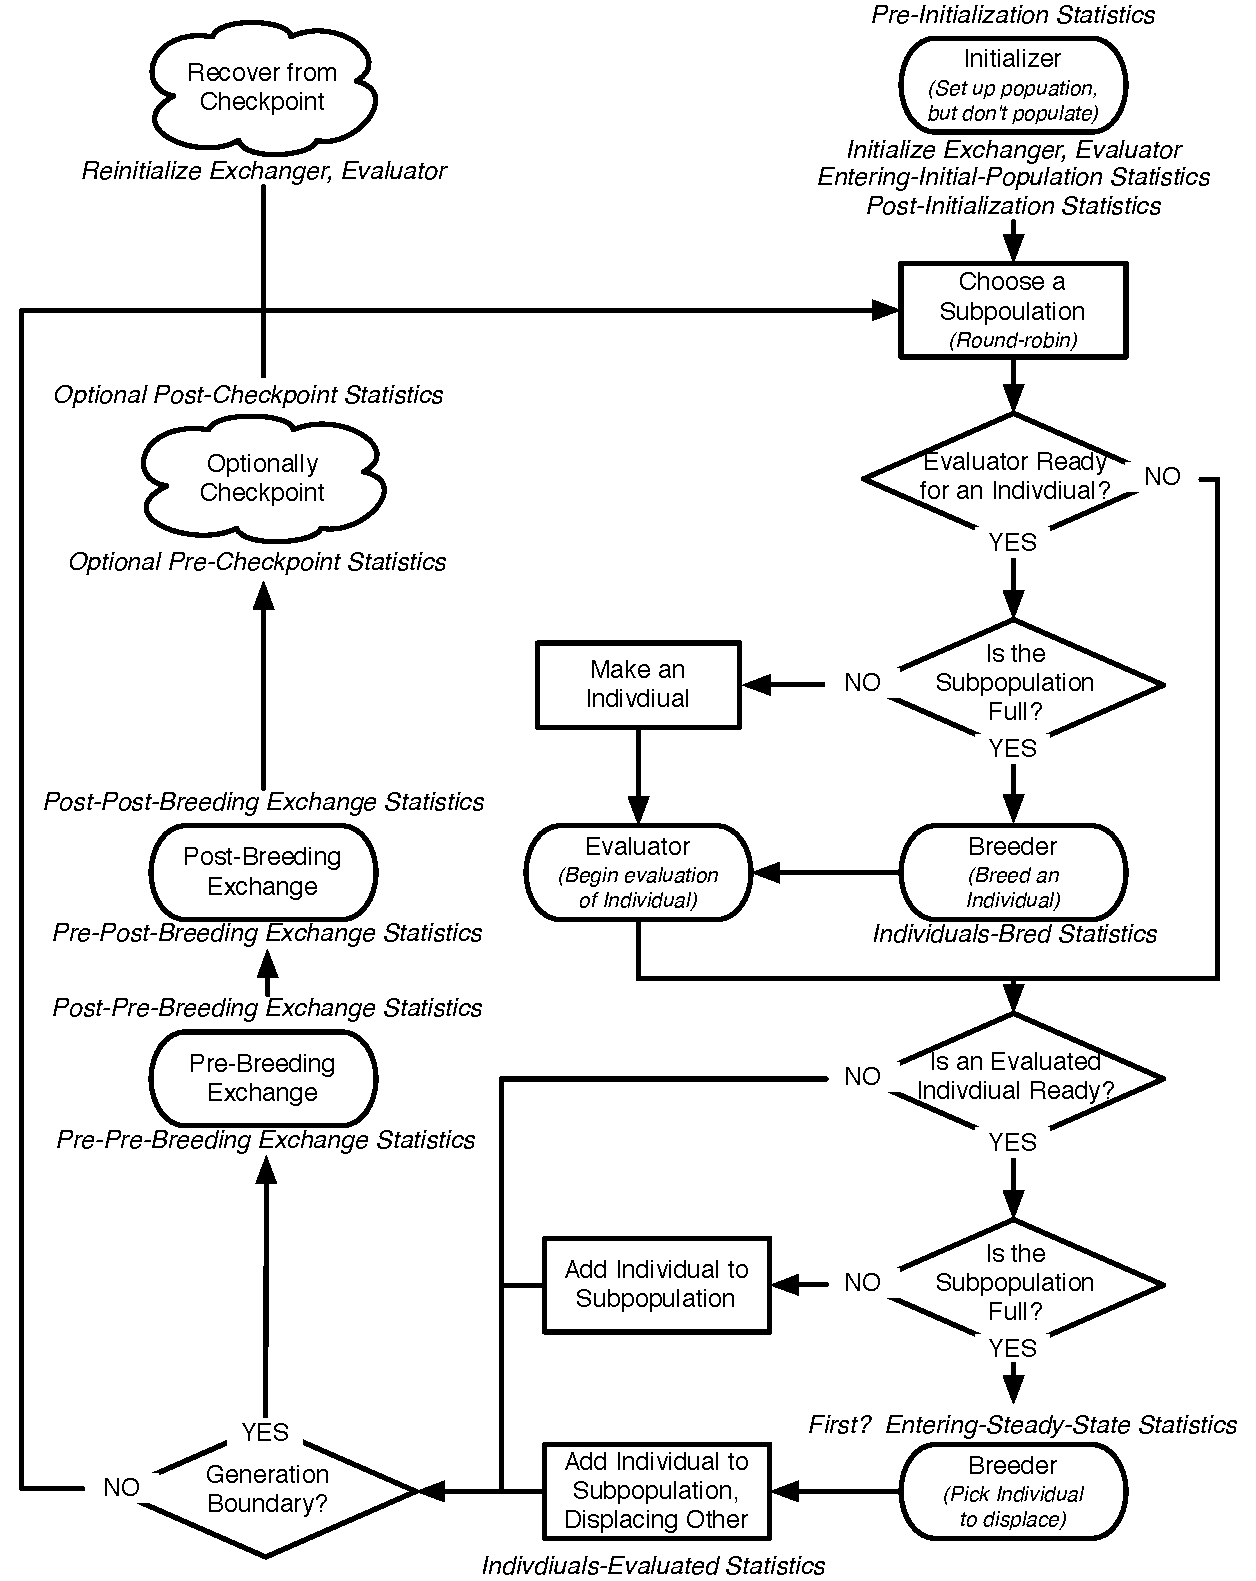
\includegraphics[height=7.5in]{SteadyState.pdf}
\end{center}
\caption{Top-Level Loop of ECJ's \class{SteadyStateEvolutionState} class, used for simple steady-state EC and Asynchronous Evolution algorithms.  {\it ``First?''} means to perform the Statistics whenever the Subpopulation in question is picking an Individual to displace for the very first time.  (Each Subpopulation will do it once, but possibly at different times).}
\label{SteadyState}
\end{figure}
\afterpage{\clearpage}


\section{Steady-State Evolution (The \package{ec.steadystate} Package)}
\label{ec.steadystate}

In Steady-state Evolution, each iteration some \(n\) individuals are breed from the existing Population, have their fitnesses assessed, and then are stuck back in the Population, displacing \(n\) others.  ECJ's implementation of Steady-State Evolution sets \(n=1\), which is the most common case.  

To implement Steady-State Evolution ECJ requires special versions of: an EvolutionState, a Breeder, and an Evaluator:

\params{%
state = ec.steadystate.SteadyStateEvolutionState\\
breed = ec.steadystate.SteadyStateBreeder\\
eval = ec.steadystate.SteadyStateEvaluator
}

Additionally Breeding Sources must adhere to certain rules, as must Exchangers and Statistics.

ECJ's top-level Steady-State Evolution loop, implemented in the class \class{ec.steadystate.SteadyStateEvolutionState}, is shown in Figure \ref{SteadyState}.  Compare to Figure \ref{EvolutionState2}, which shows a generational loop.  At this abstract level, the two are very similar: the primary differences lie in the Statistics methods called.  But inside the Breeder and Evaluator there are some significant differences.  One important detail: Steady-State Evolution {\it must} at present be single-threaded:

\params{%
evalthreads = 1\\
breedthreads = 1
}

SteadyStateEvolutionState can either run until some \(n\) evaluations have been processed, or until some \(m\) ``generations'' have been processed.  Normally SteadyStateEvolutionState uses generations.  If you'd prefer to work in evaluations, you can say something like this:

\params{%
evaluations = 10000
}

What does a ``generation'' mean in this context?  ECJ sums up the sizes of all of the subpopulations to form the {\it total population size} \(p\).  Whenever \(p\) individuals have been evaluated, that's a new generation.

Steady-State evolution in ECJ works in two stages:

\begin{itemize}
\item {\bf Stage 1: Initialization}.  The Subpopulation begins completely empty.  One-by-one, individuals are created at random and then sent off to be evaluated.  In Steady-State evolution, this evaluation happens immediately and each individual is returned immediately.  However in a distributed version called Asynchronous Evolution (discussed in Section~\ref{ec.eval}), individuals are shipped off to remote sites and may not come back for a while.  In this case evolution does not wait for them, but continues generating new individuals.

When an individual returns with its fitness assessed, it then is added to the Subpopulation until the Subpopulation is full, at which time the system advances to...

\item {\bf Stage 2: The Steady State}.  One-by-one, individuals are {\it bred} and then sent off to be evaluated.  Again, in Steady-State evolution, this evaluation happens immediately and each individual is returned immediately.  However in Asynchronous Evolution individuals are shipped off to remote sites and may not come back for a while.  In this case evolution does not wait for them, but continues breeding new individuals.

When an individual returns with its fitness assessed, an existing Subpopulation member is marked for death, and is then replaced with the new individual.  Note that if using Asynchronous Evolution, some of these new individuals may be stragglers created during Initialization.
\end{itemize}

These stages aren't immediately obvious from Figure \ref{SteadyState}: they're distinguished by both ``Is the Subpopulation Full?'' branches.

The Evaluator in question is \class{ec.steadystate.SteadyStateEvaluator}, which has no special parameters.

The Breeder in question is \class{ec.steadystate.SteadyStateBreeder}.  It contains the SelectionMethod which is used to select individuals for death.  Typically this SelectionMethod is set up to select {\it unfit} or {\it random} individuals rather than {\it fit} ones (which wouldn't make much sense).  To pick an unfit individual using Tournament Selection for Subpopulation 0, for example, we might say:

\params{%
steady.deselector.0 = ec.select.TournamentSelection\\
steady.deselector.0.size = 2\\
steady.deselector.0.pick-worst = true
}

To pick a random individual, you could change this to

\params{%
steady.deselector.0.size = 1
}

\noindent ...or you could just use...

\params{%
steady.deselector.0 = ec.select.RandomSelection
}

All BreedingSources in your breeding pipeline, and in particular SelectionMethods, must implement \class{ec.steadystate.SteadyStateBSourceForm}.  This interface contains a method called to update the BreedingSource that a new individual has entered into the population, displacing an old one.  This is important because some SelectionMethods, such as FitProportionateSelection, rely on precomputed statistics which will be no longer correct.  This method is:

\java{%
public void individualReplaced(SteadyStateEvolutionState state,\\
\hsp{\fill}int subpopulation, int thread, int individual);
}

At the very least, a BreedingSource must implement this method to call the same method on {\it its} sources.  This means that they must be of SteadyStateBSourceForm as well.  To guarantee this, the following check method must be implemented:

\java{%
public void sourcesAreProperForm(SteadyStateEvolutionState state);
}

This method should likewise call its namesake on all sources.  If the sources are not of SteadyStateBSourceForm, it should then issue an ordinary Output ``error'' (not a fatal error) indicating this problem.

SteadyStateBSourceForm is implemented by TournamentSelection and its variations; and also by FirstSelection (of course), and by RandomSelection.  You can implement SteadyStateBSourceForm for FitProportionateSelection and its ilk but it's not implemented by default because they'd be so inefficient.  I strongly suggest sticking with TournamentSelection.

Exchangers are called every {\it generation} worth of evaluations.  Since Exchangers also modify individuals in the population, they also need to update the BreedingSources of this fact.  This is done by having them call the following method in the Breeder, which lets all the relevant BreedingSources know:

\java{%
public void individualReplaced(SteadyStateEvolutionState state,\\
\hsp{\fill}int subpopulation, int thread, int individual);
}

(Yes, it's the same name).  If an Exchanger makes this promise, it gets to implement the \class{ec.steadystate.SteadyStateExchangerForm} interface as a badge of honor.

The steady state nature of evolution requires a different set of Statistics hooks.  These hooks are defined in the interface \class{ec.steadystate.SteadyStateStatisticsForm}.  Note that no ECJ Statistics class presently implements these hooks; but SteadyStateEvolutionState can handle non-SteadyStateStatisticsForm Statistics objects gracefully.

Several hooks you've already seen in Section~\ref{ec.Statistics}:

\java{%
    public void preCheckpointStatistics(EvolutionState state);\\
    public void postCheckpointStatistics(EvolutionState state);\\
    public void prePreBreedingExchangeStatistics(EvolutionState state);\\
    public void postPreBreedingExchangeStatistics(EvolutionState state);\\
    public void prePostBreedingExchangeStatistics(EvolutionState state);\\
    public void postPostBreedingExchangeStatistics(EvolutionState state);\\
    public void finalStatistics(EvolutionState state, int result);\\
}

Other hooks are special to steady-state evolution.  First, we have:

\java{%
    public void enteringInitialPopulationStatistics(\\
    \hsp{\fill}SteadyStateEvolutionState state);\\
    public void enteringSteadyStateStatistics(int subpop,\\
    \hsp{\fill}SteadyStateEvolutionState state);\\
    public void generationBoundaryStatistics(EvolutionState state); 
}

The first method is called immediately after the Population has been constructed but before any Individuals have been created.  The second method is called when a Subpopulation enters its ``steady state'', that is, it has been filled with Indivdiuals.  The third method is called whenever a generation boundary is reached, that is, when a Population's worth of individuals has been evaluated.

Last, we have two hooks which are called whenever an individual is bred or evaluated:

\java{%
    public void individualsBredStatistics(SteadyStateEvolutionState state,\\
    \hsp{\fill}Individual[] individuals);\\
    public void individualsEvaluatedStatistics(SteaPodyStateEvolutionState state,\\
  \hsp{\fill}Individual[] newIndividuals, Individual[] oldIndividuals,\\
  \hsp{\fill}int[] subpopulations, int[] indices);
}

The first method is called when one or more Individuals has just been bred (at present only one individual will be bred at a time).  The second method is called when one or more Individuals have just been evaluated and inserted into the Population, dispersing other Individuals (at present, it'll only be one individual evaluated).  The Subpopulations and Individual indices in the Subpopulations where the event occurred are provided as well. 

Last but not least, \class{ec.steady.SteadyStateDefaults} provides the package default parameter base. 

\paragraph{Example}

We again build off of the example shown in Section~\ref{ec.simple}, and continue to use generation boundaries rather than evaluations to keep things simple.  So let's use that file:

\params{%
parent.0 = ga.params
}

Steady-State evolution doesn't allow multiple threads:

\params{%
evalthreads = 1\\
breedthreads = 1
}

Next, let's override some parameters to use Steady-State Evolution:

\params{%
state = ec.steadystate.SteadyStateEvolutionState\\
breed = ec.steadystate.SteadyStateBreeder\\
eval = ec.steadystate.SteadyStateEvaluator
}

Traditionally, steady-state evolutionary algorithms try hard not to produce duplicates during initialization:

\params{%
steady.duplicate-retries = 100
}

We'll need to specify a deselector for each supopulation too. Let's do random selection:

\params{%
steady.deselector.0 = ec.select.ec.select.RandomSelection
 }
 
\noindent ...and we're done!  We don't bother changing the Statistics object.  SimpleStatistics will do in a pinch when we're observing generation boundaries.










\chapter{Representations}


\section{Vector and List Representations (The \package{ec.vector} Package)}
\label{ec.vector}

The \package{ec.vector} package defines one of the most common representations used in evolutionary algorithms: one-dimensional arrays of numbers or objects.  In Genetic Algorithms such things have often been referred to as {\bf chromosomes}.  ECJ supports Individuals consisting of a single vector of the following types:

\begin{center}
{
\small\renewcommand{\arraystretch}{1.2} 
\begin{tabular}{@{}rll@{}}
{\bf Array Type}&{\bf Individual}&{\bf Species}\\
\hline
\variable{boolean}&\class{ec.vector.BitVectorIndividual}&\class{ec.vector.VectorSpecies}\\
\variable{byte}&\class{ec.vector.ByteVectorIndividual}&\class{ec.vector.IntegerVectorSpecies}\\
\variable{short}&\class{ec.vector.ShortVectorIndividual}&\class{ec.vector.IntegerVectorSpecies}\\
\variable{int}&\class{ec.vector.IntegerVectorIndividual}&\class{ec.vector.IntegerVectorSpecies}\\
\variable{long}&\class{ec.vector.LongVectorIndividual}&\class{ec.vector.IntegerVectorSpecies}\\
\variable{float}&\class{ec.vector.DoubleVectorIndividual}&\class{ec.vector.FloatVectorSpecies}\\
\variable{double}&\class{ec.vector.DoubleVectorIndividual}&\class{ec.vector.FloatVectorSpecies}\\
Subclasses of \class{ec.vector.VectorGene}&\class{ec.vector.GeneVectorIndividual}&\class{ec.vector.GeneVectorSpecies}\\
\end{tabular}
\vspace{1em}
}
\end{center}

Note that all the integer-type Individuals (byte, short, int, long) share the same species: \class{ec.vector.IntegerVectorSpecies}.  Likewise, all the float-type Individuals (float, double) share \class{ec.vector.FloatVectorSpecies}.  Last, \class{GeneVectorIndividual} holds an array of subclasses of the abstract class \class{ec.vector.VectorGene}, which you can subclass to do or hold any data type.  All these Individuals are subclasses of the abstract class \class{ec.vector.VectorIndividual}; and all Species are subclasses of \class{ec.vector.VectorSpecies}.

Each of these Individuals has the same crossover operators and support for vector manipulation.  They differ in the default initialization and mutation mechanisms available to them: obviously Gaussian mutation makes little sense on integers, for example.

To make matters simple, ECJ has a single set of BreedingPipelines for all of these data types.  To do this, the BreedingPipelines call crossover or mutation functions in the Individuals themselves (or more properly, in their Species).  This is different from other representations and results in some breeding parameters (crossover type, mutation probability) being found in the Species and not in the BreedingPipeline in question.  But as it makes the package much smaller and simpler, so be it.

ECJ does not use generics in this package: each of the data types above has an Individual subclass all its own.  The reason for this is straightforward: generics would be {\it exceptionally} slow.  These are arrays of basic data types, and Java's generics would box and unbox them.  So no generics it is.

\subsection{Vectors}
\label{vectors}

The default use of this representation is as {\it fixed-length} vectors which can be crossed over and mutated.  The size of the vectors is specified in the Species.  For example, to define Individuals of the form of 100 bytes in Subpopulation 0, we might do this:

\params{%
pop.subpop.0.species = ec.vector.IntegerVectorSpecies\\
pop.subpop.0.species.ind = ec.vector.ByteVectorIndividual\\
pop.subpop.0.species.genome-size = 100
}

The package \package{ec.vector.breed} contains BreedingPipelines which know how to manipulate all such vectors.  Specifically:

\begin{itemize}
\item \class{ec.vector.breed.VectorMutationPipeline} takes a single source and mutates Individuals from that source by calling the \method{mutate(...)} method on them (discussed later).
\item \class{ec.vector.breed.VectorCrossoverPipeline} takes a two sources and draws one Individuals at a time each from these sources, then crosses them over by calling the \method{crossover(...)} method on one of them (discussed later).
\item \class{ec.vector.MultipleVectorCrossoverPipeline}, by Beenish Jamil, a former undergraduate at GMU, takes Individuals from a variable number of sources, then performs uniform crossover between all of them.  For example, imagine if there were three Individuals, \(A, B,\) and \(C\).  For each index \(i\), MultipleVectorCrossoverPipeline randomly shuffles the values among \(A_i, B_i,\) and \(C_i\) with a certain crossoverProbability, described next.
\end{itemize}

\subsubsection{Initialization}

VectorIndividuals are initialized by being cloned from the prototypical Individual, and then having the following method called on them:

\java{%
public void reset(EvolutionState state, int thread);
}

How VectorIndividuals implement this method depends on their type:

\begin{itemize}
\item {\bf Floating Point} (\variable{float, double}):  each gene is set to a random value between its legal minimum and maximum values, inclusive.
\item {\bf Integer} (\variable{byte, short, int, long}):  each gene is set to a random value between its legal minimum and maximum values, inclusive.
\item {\bf Boolean}:  each gene is set to a random value.
\item {\bf Gene}:  each gene is randomized by calling the following method on its \class{ec.vector.VectorGene}:

\java{%
public void reset(EvolutionState state, int thread);
}
\end{itemize}

Floating Point and Integer individuals need minimum and maximum values for their genes.  These values can be set in any combination of three ways:

\begin{itemize}
\item Global settings for the entire Individual.  For example:

\params{%
pop.subpop.0.species.min-gene = -14\\
pop.subpop.0.species.max-gene = 92
}

\item Settings for {\it segments} along the Individual.   The number of segments is:

\params{%
pop.subpop.0.species.num-segments = 4
}

Segments may be either specified by stating the {\it start indices} of each segment:

\params{%
pop.subpop.0.species.segment-type = start\\
\\
pop.subpop.0.species.segment.0.start = 0\\
pop.subpop.0.species.segment.1.start = 15\\
pop.subpop.0.species.segment.2.start = 50\\
pop.subpop.0.species.segment.3.start = 80
}

\noindent ... or they may be specified by stating the {\it end indices} of each segment.\footnote{Why do this?  It's a long story, with no good excuses.} 

\params{%
pop.subpop.0.species.segment-type = end\\
\\
pop.subpop.0.species.segment.0.end = 14\\
pop.subpop.0.species.segment.1.end = 49\\
pop.subpop.0.species.segment.2.end = 79\\
pop.subpop.0.species.segment.3.end = 100
}

Then we specify the min and max gene values for all genes in each segment:

\params{%
pop.subpop.0.species.segment.0.min-gene = -14\\
pop.subpop.0.species.segment.0.max-gene = 92\\
pop.subpop.0.species.segment.1.min-gene = 0\\
pop.subpop.0.species.segment.1.max-gene = 100\\
pop.subpop.0.species.segment.2.min-gene = 0\\
pop.subpop.0.species.segment.2.max-gene = 50\\
pop.subpop.0.species.segment.3.min-gene = -0\\
pop.subpop.0.species.segment.3.max-gene = 1
}

The code for segments was provided by Rafal Kicinger, then a PhD student at GMU.

\item Last, settings for {\it individual genes} may be stated.  Not all genes have to be stated this way, just the ones you want.  For example:

\params{%
pop.subpop.0.species.min-gene.59 = 2\\
pop.subpop.0.species.max-gene.59 = 26\\
pop.subpop.0.species.min-gene.72 = 3\\
pop.subpop.0.species.max-gene.59 = 19
}
\end{itemize}

The rule is: individual gene settings override segment settings, which in turn override global settings.

\subsubsection{Crossover}

The class \class{ec.vector.breed.VectorCrossoverPipeline} works by calling the following method on one of the Individuals, passing in the other:

\java{%
public void defaultCrossover(EvolutionState state, int thread,\\
\hsp{\fill}VectorIndividual ind);
}

The two Individuals must be of the same type.  You could override this method in a custom VectorIndivdual of some sort to do your own crossover type.

All VectorIndividuals have default implementations of this method, which follow parameters specified in their Species.  The first thing to know about crossover in vectors is that most forms (one-point, two-point, uniform) only occur along {\bf chunk boundaries}.  By default chunks are the size of a single gene; but you can make them larger.  For example, you could specify that crossover can only occur every seven bytes in our ByteVectorIndivdiual:

\params{%
pop.subpop.0.species.chunk-size = 7
}

Why would you do this?  Mostly because you have encoded genes such that groups of seven genes together constitute a unit of some sort which shouldn't be broken up arbitrarily via crossover.

ECJ's \class{ec.vector.breed.VectorCrossoverPipeline} supports five typoes of crossover.  The crossover type is specified like this:

\params{%
pop.subpop.0.species.crossover-type = one-point
}

The types are:

\begin{itemize}
\item \parameter{one-point} performs standard One-Point crossover.
\item \parameter{two-point} performs standard Two-Point crossover.
\item \parameter{uniform} performs parameterized Uniform crossover, where every gene is crossed over independently with a certain probability.  \class{ec.vector.MultipleVectorCrossoverPipeline} also uses this probability.  The probability is stated like this:

\params{%
pop.subpop.0.species.crossover-prob = 0.25
}

(It doesn't make sense to use a probability over 0.5).  It's important to note that the \parameter{crossover-probability} parameter is the the {\it per-gene} crossover probability, not the probability that the {\it entire individual} will be crossed over.  For that, see the \parameter{likelihood} parameter in Section~\ref{breeders}.

\item \parameter{line} performs Line Recombination.  {\LARGE\bf Look up who wrote this}  The two individuals are treated as points in space.  A straight line is drawn through both points, and two children are created along this line.  If the individuals are \(\vec{x}\) and \(\vec{y}\), we draw two random values \(\alpha\) and \(\beta\), each between \(-p\) and \(1+p\) inclusive.  Then the two children are defined as \(\alpha \vec{x} + (1-\alpha) \vec{y}\) and \(\beta \vec{y} + (1-\beta) \vec{x}\) respectively.  For Integer vector individuals, the values of each index are then rounded to the nearest integer. The most common setting of \(p\) is 0.25, which allows children to be somewhat outside the hypercube formed with the parents at corners.  To set the value of \(p\), we state:

\params{%
pop.subpop.0.species.line-extension = 0.25
}

Line Recombination cannot be performed on BitVectorIndivdiuals or GeneVectorIndividuals.   ECJ's implementation of Line Recombination is due to William Haddon, a former student at GMU.

\item \parameter{intermediate} performs Intermediate Recombination.  This is very similar to Line Recombination.  The two individuals are again treated as points in space.  Children are created somewhere in the vicinity of the hypercube formed with the two individuals as corners.   If the individuals are \(\vec{x}\) and \(\vec{y}\), {\it for every index \(i\)} we draw two independent random values \(\alpha_i\) and \(\beta_i\), each between \(-p\) and \(1+p\) inclusive.  Then genes at index value \(i\) of the two children are defined as \(\alpha_i x_i + (1-\alpha_i) y_i\) and \(\beta_i y_i + (1-\beta_i) x_i\) respectively.  For Integer vector individuals, the values of each index are then rounded to the nearest integer.  Again, the most common setting of \(p\) is 0.25, which allows children to be somewhat outside the hypercube formed with the parents at corners.  Again, to set the value of \(p\), we state:

\params{%
pop.subpop.0.species.line-extension = 0.25
}

Intermediate Recombination cannot be performed on BitVectorIndivdiuals or GeneVectorIndividuals.   ECJ's implementation of Intermediate Recombination is also due to William Haddon.

\item \parameter{sbx} performs Simulated Binary Crossover.  This crossover, by Kalyanmoy Deb, attempts to simulate the effect of binary crossover on doubles and floats as if they were encoded as bits.  It relies on the Polynomial Distribution and as such has a parameter called the {\it crossover distribution index} which specifies the kind of distribution.  The standard accepted value for this index is 20 (but it's not the ECJ default: you must set it):

\params{%
pop.subpop.0.species.crossover-distribution-index = 20
}

You can use any integer \(\geq 0\).  There are probably several different versions of SBX out there.  The implementation in ECJ is a faithful reproduction of the one which appears in the NSGA-II C code found here:  http://www.iitk.ac.in/kangal/codes/nsga/nsgaorig.tar
 
\end{itemize}

VectorCrossoverPipeline can be set to return both crossed-over children or just one of them.  This parameter isn't in the Species but is actually in the Pipeline proper.  Let's say that VectorCrossoverPipeline was the root Pipeline for Subpopulation 0.  To set it to return just one child, you'd say:

\params{%
pop.subpop.0.species.pipe = ec.vector.breed.VectorCrossoverPipeline
pop.subpop.0.species.pipe.toss = true
}

Alternatively you could use the default base:

\params{%
vector.xover.toss = true
}

The default value is false.

\subsubsection{Multi-Vector Crossover}

The class \class{ec.vector.MultipleVectorCrossoverPipeline} performs uniform crossover among the Indivdiuals in question as described earlier.  It ignores the \parameter{crossover-type} parameter, but it does respect, and indeed require, the parameter:

\params{%
pop.subpop.0.species.crossover-prob = 0.25
}

This is the probability that a given gene index will be shuffled among the various Individuals.  As before, it doesn't make much sense for this to be set to any value over 0.5.

\subsubsection{Mutation}

Similarly, the BreedingPipeline \class{ec.vector.breed.VectorMutationPipeline} does its work by calling the following method on the Individual in question:

\java{%
public void defaultMutate(EvolutionState state, int thread);
}

You could override this method in a custom VectorIndivdual of some sort to do your own custom kind of mutation.

Every VectorIndivdiual has a default implementation of this method.  Mutation parameters are also specified in the Species of each Individual. At present the default mutation procedures do not respect chunk boundaries, unlike Crossover.  However, each gene is only mutated with a certain probability.  This probability is defined as:

\params{%
pop.subpop.0.species.mutation-probability = 0.1
}

Different representations have different kinds of mutations.  Specifically:


\begin{itemize}

\item {\bf Boolean} (\variable{boolean}): the default mutation operator simply flips the boolean value with the given mutation probability.

\item {\bf Integer} (\variable{byte, short, int, long}): the default mutation operator simply randomizes the integer value between the legal minimum and maximum values (with the mutation probability of course).  There are almost certainly smarter approaches than this\,---\,you'll probably want to implement something in a subclass.

\item {\bf Gene}: the default mutation operator for \class{ec.vector.GeneVectorIndividual}, with the given mutation probability, calls the following VectorGene method:

\java{%
public void mutate(EvolutionState state, int thread);
}

You are responsible for implementing this method.    The default version of the method calls:

\java{%
public void reset(EvolutionState state, int thread);
}

\noindent ...on the VectorGene.
\item {\bf Floating Point} (\variable{float, double}): allows uniform gene randomization (\parameter{reset}), Gaussian mutation (\parameter{gauss}), or Polynomial mutation(\parameter{polynomial}).  

\paragraph{Uniform Mutation}
Uniform gene randomization simply sets the gene to a random value between its minimum and maximum legal values.  To use it, you say:

\params{%
pop.subpop.0.species.mutation-type = reset
}

\paragraph{Gaussian Mutation}
Gaussian mutation adds Gaussian noise to the current value.  If the result is outside the bounds of minimum and maximum legal values, another Gaussian noise is tried instead, and so on, until a legal value is found.  You will need to specify a standard deviation for the Gaussian random noise and also the number of times ECJ should attempt to apply Gaussian noise within the minimum and maximum bounds before giving up and simply keeping the original value.  For example:

\params{%
pop.subpop.0.species.mutation-type = gauss\\
pop.subpop.0.species.mutation-stdev = 0.1\\
pop.subpop.0.species.out-of-bounds-retries = 20
}

Note that if \parameter{out-of-bounds-retries} is 0, then ECJ behaves specially: it never stops retrying.  The default value is 100.

Alternatively you can add Gaussian noise to the current values and simply allow the results to freely exceed the min/max gene bounds.  No retries are attempted (and \parameter{out-of-bounds-retries} is ignored): noise is simply added and that's it.  If you do this, be certain that the particular problem you're testing works properly with values outside the stated initial bounds.  To lift the bounds in this way, you say:

\params{%
pop.subpop.0.species.mutation-bounded = false
}

This does not affect the use of gene bounds in determining initialization values.  Even if you declare the mutation to be bounded, you'll still need to provide \parameter{out-of-bounds-retries} (though it won't be used).

\paragraph{Polynomial Mutation}
Finally, Polynomial mutation is by Kalyanmoy Deb, and uses a distribution chosen from the Polynomial distribution series rather than a Gaussian distribution.  All Polynomial distributions have a min and max value ranging in [-1, 1], and Polynomial mutation adjusts this to reflect the min and max gene ranges.   The Polynomial distribution used is defined by the {\it distribution index} and by far the most common setting (but not the ECJ default) is 20.  There are at least four different versions of Polynomial mutation in the literature or various common code.  We have implemented two versions: the {\bf standard} version, which can produce values outside the min/max range, and an {\bf alternative} version found in the NSGA-II C code among certain other places (http://www.iitk.ac.in/kangal/codes/nsga/nsgaorig.tar), which modifies the distribution to always mutate values within the min/max range. Note that we've found the alternative version superior for multiobjective optimization problems.  In ECJ, {\bf the alternative version is the default.} 

To use the {\it alternative} version, you'll need to state something like this.

\params{%
pop.subpop.0.species.mutation-type = polynomial\\
pop.subpop.0.species.mutation-distribution-index = 20\\
pop.subpop.0.species.alternative-polynomial-version = true\\
pop.subpop.0.species.out-of-bounds-retries = 20
}

You can use any integer \(\geq 0\) for the distribution index.  Note that even though the alternative version doesn't actually need \parameter{out-of-bounds-retries}, ECJ requires it anyway, so just put something arbitrary there.

To use the {\it standard} version, you'll need to state something along these lines.

\params{%
pop.subpop.0.species.mutation-type = polynomial\\
pop.subpop.0.species.mutation-distribution-index = 20\\
pop.subpop.0.species.alternative-polynomial-version = false\\
pop.subpop.0.species.out-of-bounds-retries = 20
}

Here you'll need to provide a rational value for \parameter{out-of-bounds-retries}.

Just as was the case for Gaussian noise, you have the option of lifting the bounds entirely and letting Polynomial Mutation freely exceed the min/max gene bounds.  In this case, no retries are attempted (and \parameter{out-of-bounds-retries} is ignored): noise is simply added and that's it.  Again, if you do this, be certain that the particular problem you're testing works properly with values outside the stated initial bounds.  To lift the bounds in this way, you say:

\params{%
pop.subpop.0.species.mutation-bounded = false
}

Once again, this does not affect the use of gene bounds in determining initialization values.  And even if you declare the mutation to be bounded, you'll still need to provide \parameter{out-of-bounds-retries} (though it won't be used).
\end{itemize}

Numeric representations (integer, floating-point) provide two utility methods which may be useful to you in creating or debugging a custom mutator:

\java{%
public boolean isInRange();\\
public void clamp();
}

The first method returns true if all the genes in the representation are within their minimum and maximum per-gene bounds.  The second method insures that this is the case: if a gene is larger than its maximum, it is set to the maximum; and if it is smaller than the minimum, it is set to the minimum.





\paragraph{Example}

In the Genetic Algorithms section (Section~\ref{ec.simple}), we provided an example for a pipeline for crossing over and mutating VectorIndividuals:

\params{%
pop.subpop.0.species.pipe = ec.vector.VectorMutationPipeline\\
pop.subpop.0.species.pipe.source.0 = ec.vector.VectorCrossoverPipeline\\
pop.subpop.0.species.pipe.source.0.source.0 = ec.select.TournamentSelection\\
pop.subpop.0.species.pipe.source.0.source.1 = same\\
select.tournament.size = 2
}

The example used IntegerVectorIndividuals.  Let's change it to DoubleVectorIndividuals, and also specify some constraints.

\params{%
pop.subpops.0.species = ec.vector.FloatVectorSpecies\\
pop.subpop.0.species.ind = ec.vector.DoubleVectorIndividual\\
pop.subpop.0.species.genome-size = 100
}

Let's also add some minimum and maximum gene information, both globally and for the first gene:

 \params{%
pop.subpops.0.species.min-gene = 0.0\\
pop.subpops.0.species.max-gene = 1.0\\
pop.subpops.0.species.min-gene.0 = 0.0\\
pop.subpops.0.species.max-gene.0 = 2.0
}

We'll do gaussian mutation with 100\% likelihood, and some uniform crossover:

\params{%
pop.subpop.0.species.crossover-type = uniform\\
pop.subpop.0.species.crossover-prob = 0.25\\
pop.subpop.0.species.mutation-prob = 1.0\\
pop.subpop.0.species.mutation-type = gauss\\
pop.subpop.0.species.mutation-stdev = 0.1
}

\paragraph{Another Example}

Bit vectors used to be very common.  Let's change our Individual to one.  Note that it uses \class{ec.vector.VectorSpecies} as its Species:

\params{%
pop.subpops.0.species = ec.vector.VectorSpecies\\
pop.subpop.0.species.ind = ec.vector.BooleanVectorIndividual\\
pop.subpop.0.species.genome-size = 128
}

Perhaps our encoding uses each 32 bits to represent some important concept, so we'd like to prevent crossover from occurring anywhere except on 32-bit boundaries:

 \params{%
pop.subpops.0.species.chunk-size = 32
}

Booleans only have one mutation parameter: probability of bit-flip.  Let's also include two-point crossover on the chunk boundaries:

\params{%
pop.subpop.0.species.crossover-type = one\\
pop.subpop.0.species.mutation-prob = 0.01
}




\subsection{Lists}
\label{list}

While vectors are arrays of fixed length, Lists are arrays of arbitrary and possibly changing length.  List representations are much less common in evolutionary algorithms.  

With a few changes, the classes in ECJ's \package{ec.vector} package may be used for lists as well as for vectors.  ECJ supports list representations in four ways:

\begin{itemize}
\item Useful utility methods for manipulating lists.
\item List-oriented initialization
\item List-oriented crossover procedures.
\item Default vector mutation also works fine for lists.
\end{itemize}

Let's cover each in turn.  But first read the previous section on Vectors (Section~\ref{vectors}).  And note that lists completely ignore the chunk facility: it's to complex.  

\subsubsection{Utility Methods}
VectorIndividual provides methods for manipulating the genome without knowing the type of the object in question  First, the genome (the array) may be retrieved and set:

\java{%
public Object getGenome();\\
public void setGenome(Object genome);
}

Second, the genome length can be changed.  If the length is shortened, the array will be truncated.  If the length is lengthened, the extra area will be set as follows: boolean array slots will be set to \variable{false}.  Numeric array slots will be set to 0.  VectorGene array slots will be set to a blank VectorGene cloned from the prototype.  The methods for checking or changing the length are:

\java{%
public int size();\\
public int genomeLength();\\
public void setGenomeLength(int length);\\
public void reset(EvolutionState state, int thread, int newSize);
}

The first to methods are synonymous.  The last method resizes the individual, then resets it entirely (randomizes its values).

Third, VectorIndividual supplies methods for cutting a splicing genome arrays, which is quite useful for manipulating variable-length lists.  For example, you can {\bf split} a genome into some \(n\) pieces.  To do this you provide \(n-1\) split points.  The first piece will start at index 0 and run up to, but not including, the first split point; the second piece will start with the spit point and run up to, but not including, the second split point;  and so on.  The final piece will run to the end of the genome.  The \(n\) pieces are placed into the provided Object array.

\java{%
public void split(int[] points, Object[] pieces);
}

VectorIndividual can also {\bf join} certain pieces\,---\,concatenate them\,---\,to form the genome, replacing the original genome.

\java{%
public void join(Object[] pieces);
}

Last, VectorIndividual can clone genes in the arrays split off of a genome before joining them again.  This is useful for concatenating genes to an Individual for example.  Obviously, genomes consisting of arrays of numbers or booleans don't need to be ``cloned''\,---\,but the \class{VectorGene}s found in \class{GeneVectorIndividual} need to be copied or else the concatenated gene slots will share pointers with the original genes, which you perhaps didn't want.  Note that the \variable{pieces} array is modified in place.

\java{%
public void cloneGenes(Object[] pieces);
}


\subsubsection{Initialization}

The initial size of the genome can be hard-coded in parameters (just like it was for vectors), or you can specify one of two algorithms for picking a size.  To hard-code the size, just do it like a vector:

\params{%
pop.subpop.0.species.genome-size = 100
}

Alternatively you can ask ECJ to pick the genome size uniformly from between a minimum and maximum size inclusive:

\params{%
pop.subpop.0.species.genome-size = uniform\\
pop.subpop.0.species.min-initial-size = 10\\
pop.subpop.0.species.max-initial-size = 80
}

Last, you can ask ECJ to pick the genome size from the geometric distribution.  Here ECJ will start at the minimum size, then flip a coin of a given probability.  If the coin comes up heads (true), ECJ will increase the size by one, then flip the coin again, and so on, until the coin comes up tails (false).  That'll be the resulting size.  For this you need to provide the probability and the minimum size:

\params{%
pop.subpop.0.species.genome-size = geometric\\
pop.subpop.0.species.min-initial-size = 10\\
pop.subpop.0.species.geometric-prob = 0.95
}

\subsubsection{Crossover}

In the \package{ec.vector.breed} package is one special pipeline made for crossing over lists, called, not surprisingly, \class{ec.vector.breed.ListCrossoverPipeline}.  This class was developed by Stephen Donnelly, then an undergraduate at GMU.

ListCrossoverPipeline performs either one-point or two-point list crossover.  In one-point list crossover, we pick random indexes \(i\) and \(j\) in each of two individuals \(A\) and \(B\) (which may have different lengths).  We then swap the string of genes \(A_i, ..., A_{\textit{end}}\) and \(B_j, ..., B_{\textit{end}}\).  It's possible for these strings to be all of the Individual, or entirely empty.

In two-point list crossover, for each individual we pick {\it two} random indexes: \(i \leq j\) for Individual \(A\) and \(k \leq l\) for Individual \(B\).  We then swap the string of genes \(A_i, ..., A_j\) with \(B_k, ..., B_l\).   Again, it's possible for these strings to be all of the Individual, or entirely empty.

You specify the form of crossover like you do with Vectors: in the Species.  

\params{%
pop.subpop.0.species.crossover-type = one-point
}

(or \parameter{two-point}, if you prefer).

ListCrossoverPipeline's crossover can be constrained in several ways.  First, you can stipulate that the children are no less than a certain size.  Let's say that ListCrossoverPipeline was the root Pipeline for Subpopulation 0.  To set it to never return children less than 5 in length, you might say:

\params{%
pop.subpop.0.species.pipe = ec.vector.breed.ListCrossoverPipeline\\
pop.subpop.0.species.pipe.min-child-size = 5
}

The default is 0. 

To set it to never remove more than a certain percentage, and no less than another percentage, of material from a parent, you could say:

\params{%
pop.subpop.0.species.pipe.min-crossover-percent = 0.25\\
pop.subpop.0.species.pipe.max-crossover-percent = 0.50
}

The defaults are 0.0 and 1.0 respectively.

ListCrossoverPipeline will try repeatedly to find crossover points which met these constraints.  If it fails, it will simply return the two parents.  You set the number of times it will try like this:

\params{%
pop.subpop.0.species.pipe.tries = 100
}

The default is 1.

Like VectorCrossoverPipeline, ListCrossoverPipeline can be set to return both crossed-over children or just one of them.  To set it to return just one child, you'd say:

\params{%
pop.subpop.0.species.pipe.toss = true
}

The default value is false.

Alternatively you could use the default base for any or all of these:

\params{%
vector.list-xover.min-child-size = 5\\
vector.list-xover.min-crossover-percent = 0.25\\
vector.list-xover.max-crossover-percent = 0.50\\
vector.list-xover.tries = 100\\
vector.list-xover.toss = true
}




\subsubsection{Mutation}

The standard vector mutation operator will work fine in list mode: it doesn't care what the length of the array is.

ECJ at present has a single mutation operators special to lists: \class{ec.vector.breed.GeneDuplicationPipeline}.  This pipeline replicates a particular mutation operation common in Grammatical Evolution (Section \ref{ec.gp.ge}).  Specifically: we select two indices in the list at random such that they are not equal to one another.  Then we copy the region between the two indices, and concatenate it to the end of the list.  And that's it!

\paragraph{Example}

Let's modify the Vector example given previously.  First, we'll change the crossover procedure:

\params{%
pop.subpop.0.species.pipe = ec.vector.VectorMutationPipeline\\
pop.subpop.0.species.pipe.source.0 = ec.vector.ListCrossoverPipeline\\
pop.subpop.0.species.pipe.source.0.source.0 = ec.select.TournamentSelection\\
pop.subpop.0.species.pipe.source.0.source.1 = same\\
select.tournament.size = 2
}

Let's stipulate that crossed-over individuals must be at least two genes in length if possible:

\params{%
pop.subpop.0.species.pipe.source.0.min-child-size = 2
}

Finally, let's change the procedure for determining the initial size of an Individual:

\params{%
pop.subpop.0.species.genome-size = geometric\\
pop.subpop.0.species.min-initial-size = 10\\
pop.subpop.0.species.geometric-prob = 0.95
}



\subsection{Arbitrary Genes: \class{ec.vector.VectorGene}}

Last, some discussion should be reserved regarding vectors of ``arbitrary genes''.  The idea behind this is to provide you with maximum flexibility as to what you can create vectors out of.  The classes involved here are:

\begin{itemize}
\item \class{ec.vector.VectorGene}, the abstract superclass of objects which can fill gene positions.
\item \class{ec.vector.GeneVectorIndividual}, the VectorIndividual which contains nothing but VectorGenes.
\item \class{ec.vector.GeneVectorSpecies}, the Species for GeneVectorIndividuals.
\end{itemize}

To use these classes, you'll not only need to specify the use of GeneVectorIndividual and GeneVectorSpecies, but you'll also need to state which subclass of VectorGene will be used to fill the GeneVectorIndividual.  These three things are done as follows:

\params{%
pop.subpop.0.species = ec.vector.GeneVectorSpecies\\
pop.subpop.0.species.ind = ec.vector.GeneVectorIndividual\\
pop.subpop.0.species.gene = ec.app.MySubclassOfVectorGene
}

As mentioned earlier, GeneVectorIndividual's \method{reset(...)} method, used to initialize the Individual, in turn calls this method on your VectorGene subclass:

\java{%
public abstract void reset(EvolutionState state, int thread);
}

Furthermore, mutation on GeneVectorIndividuals call this method on each VectorGene (with the mutation probability):

\java{%
public abstract void mutate(EvolutionState state, int thread);
}

The default form of this method just calls \method{reset(...)}.

VectorGene is a Prototype, and so requires \method{setup(...)}, \method{clone(...)}, and \method{defaultBase()}.  Default implementations are already provided for you.  Except for \method{clone(...)} you're unlikely to need to override them.

You do need to provide two additional VectorGene methods:

\java{%
public abstract int hashCode();\\
public abstract boolean equals(Object other);
}

The first method should provide an intelligent hash code based on the value of the VectorGene contents.  The second method should test this VectorGene against another for equality and return true if they contain the same thing.

Technically that's all you need to provide.  But in reality VectorGene is not going to be very useful unless you at least provide a way to describe the gene when it's printed to a log.  The easiest way to do this is to override this method:

\java{%
    public String printGeneToStringForHumans();
}

The default version of this method simply calls \method{toString()} (which you could override too if you wanted).  This method is in turn called by 

\java{%
    public void printGeneForHumans(EvolutionState state, int verbosity, int log);
}

If you're writing Individuals with the intent that they be read back in again later, you'll probably want to override this method:

\java{%
public String printGeneToString();
}

This method is called in turn by the following two methods:

\java{%
    public void printGene(EvolutionState state, int verbosity, int log);\\
    public void printGene(EvolutionState state, PrintWriter writer);
}

The default form simply calls \method{toString()}, which is definitely wrong.  You'll also want to override the method which reads in the gene again:

\java{%
    public void readGeneFromString(String string, EvolutionState state);
}

To write out the gene in a computer-readable fashion, I suggest using ECJ's Code package (Section~\ref{ec.util.Code}), but it's up to you.  This method is called by 

\java{%
public void readGene(EvolutionState state, LineNumberReader reader)\\
\hsp{\fill}throws IOException;
}

Finally if you're intending to send your Individual over the network, either for distributed evaluation or island models, you'll need to implement these methods:

\java{%
    public void writeGene(EvolutionState state, DataOutput output)\\
\hsp{\fill}throws IOException;\\
    public void readGene(EvolutionState state, DataInput input) throws IOException;
}

\paragraph{Example}

The following VectorGene contains two doubles and mutates them by performing a random affine rotation on them (why not?).  We'll implement it fully here, though keep in mind that this isn't entirely necessary.  For fun, we'll use an elaborate hash code which XORs all four 32-bit segments of the two doubles together (I hope I wrote that right!).

First the parameters:

\params{%
pop.subpop.0.species = ec.vector.GeneVectorSpecies\\
pop.subpop.0.species.ind = ec.vector.GeneVectorIndividual\\
pop.subpop.0.species.gene = ec.app.trig.TrigGene
}

Now the implementation:

\vbox{
\small\begin{verbatim}
package ec.app.trig;
import ec.util.*;
public class TrigGene extends VectorGene {
    double x;
    double y;
    public void reset(EvolutionState state, int thread) {
        double alpha = state.random[thread].nextDouble() * Math.PI * 2;
        x = Math.cos(alpha);     y = Math.sin(alpha);
        }
        
    public void mutate(EvolutionState state, int thread) {
        double alpha = Math.atan2(y,x);
        double dalpha = (state.random[thread].nextDouble() - 0.5) * Math.PI * 2 / 100.0;
        x = Math.cos(alpha + dalpha);     y = Math.sin(alpha + dalpha);
        }
        
    public int hashCode() {
        long a = Double.doubleToRawLongBits(x);  long b = Double.doubleToRawLongBits(y);
        return (int) ((a & (int)-1) ^ (a >> 32) (b & (int)-1) ^ (b >> 32));
        }

    public boolean equals(Object other) {
        return (other != null && other instanceof TrigGene &&
                ((TrigGene)other).x == x && ((TrigGene)other).y == y); 
        }
        
    public String printGeneToStringForHumans() { return ">" + x + " " + y ;  }
    
    public String printGeneToString() {
        return ">" + Code.Encode(x) + " " + Code.Encode(x);
        }

    public void readGeneFromString(String string, EvolutionState state) {
        string = string.trim().substring(0);  // get rid of the ">"
        DecodeReturn dr = new DecodeReturn(string);
        Code.decode(dr);  x = dr.d;           // no error checking
        Code.decode(dr);  y = dr.d;
        }
        
    public void writeGene(EvolutionState state, DataOutput out) throws IOException {
        out.writeDouble(x);  out.writeDouble(y);
        }

    public void readGene(EvolutionState state, DataOutput in) throws IOException {
        x = in.readDouble(); y = in.readDouble();
        }
    }
\end{verbatim}
}


\begin{figure}
\begin{center}
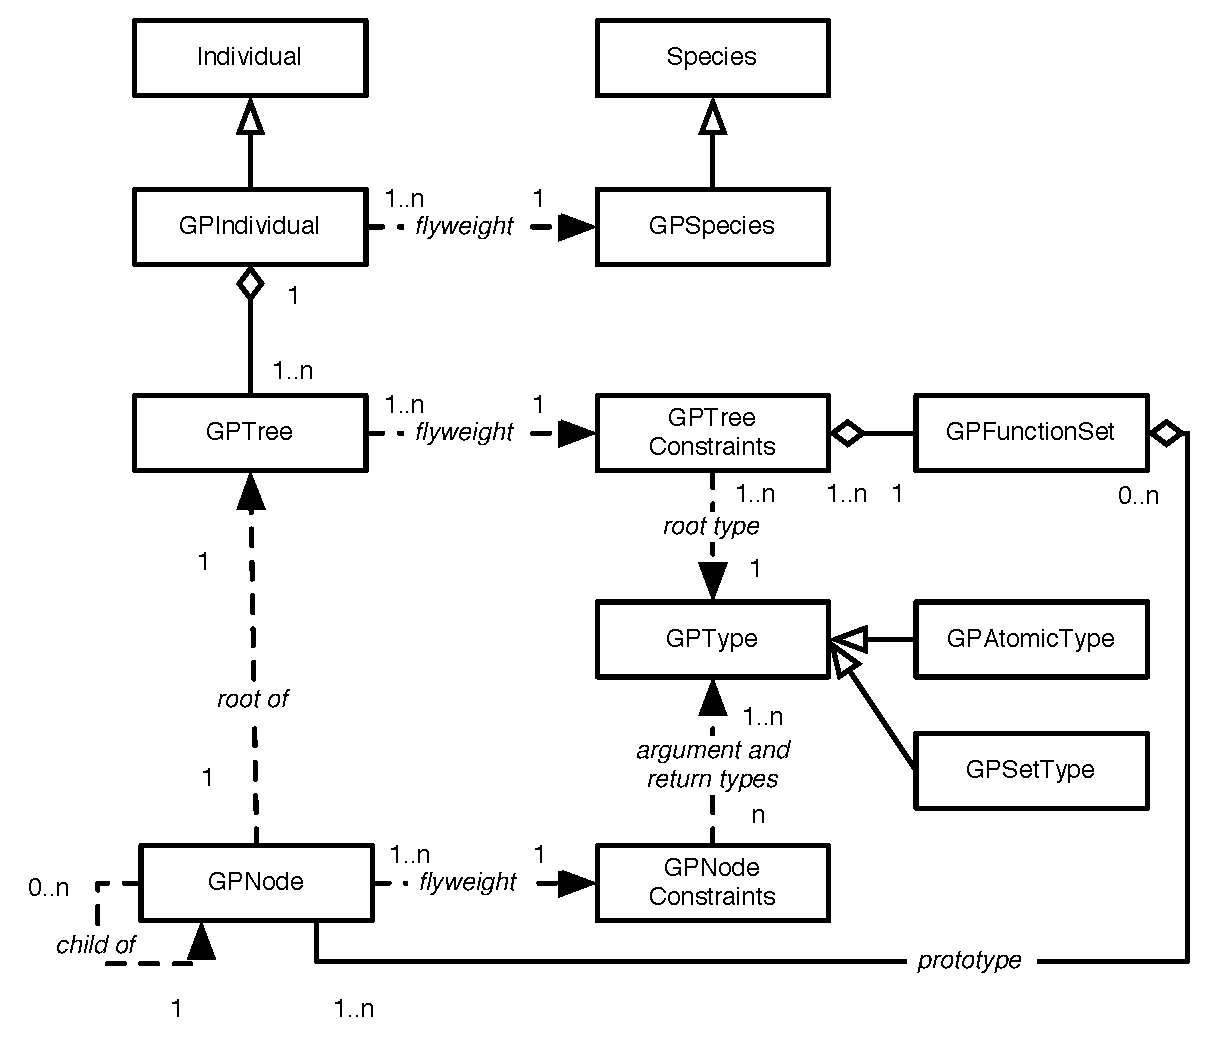
\includegraphics[width=6.5in]{GP.pdf}
\end{center}
\caption{Data objects common to tree-based ``Koza-style'' genetic programming Individuals.}
\label{GP}
\end{figure}


\section{Genetic Programming (The \package{ec.gp} Package)}
\label{ec.gp}

The \package{ec.gp} package is far and away the most developed and tested package in ECJ.  ECJ was largely developed in order to support his package, and much of our existing literature is based on it.

ECJ's genetic programming package uses ``Koza-style'' tree structures \cite{koza:book,koza:gp2} which represent the parse trees of Lisp s-expressions.   For an introduction to genetic programming, see \cite{poli08:fieldguide}.  Much of ECJ's approach to GP is inspired by {\it lil-gp} \cite{lilgp}, an earlier C-based GP system.  However {\it lil-gp} and many other GP systems pack the parse trees into arrays to save memory.  ECJ does not: the parse trees are stored as tree structures in memory.  This is much more wasteful of memory but it is faster to evaluate and far easier to manipulate.

GP's top-level class is an Individual called \class{ec.gp.GPIndividual}.  GPIndividual holds an array of GP trees, held by \class{ec.gp.GPTree} objects.  Each GP tree is a tree of \class{ec.gp.GPNode} objects.  One GPNode, the root of the tree, is held by the GPTree.

GPIndividual, GPTree, and GPNode are all Prototypes, and furthermore they all adhere to the {\it flyweight} pattern (Section~\ref{flyweight}).  GPIndividual's flyweight relationship is with a Species (of course), called \class{ec.gp.GPSpecies}.  GPTrees have a flyweight relationship with subclasses of \class{ec.gp.GPTreeConstraints}.  GPNodes have a flyweight relationship with subclasses of \class{ec.gp.GPNodeConstraints}.

GP's tree nodes are {\bf typed}, meaning that they can have certain constraints which specify which nodes may serve as children of other nodes.  These types are defined by an abstract class called \class{ec.gp.GPType}, of which there are two concrete subclasses, \class{ec.gp.GPAtomicType} and \class{ec.gp.GPSetType}.

The primary function of GPSpecies is to build new GPIndividuals properly.  The primary function of GPTreeConstraints is to hold onto the {\bf function set} (\class{ec.gp.GPFunctionSet}) for a given tree.  This is a set of prototypical GPNodes, copies of which are used to construct the tree in question.  GPTreeConstraints also contains typing information for the tree root.  The primary purpose of GPNodeConstraints is to provide typing and arity information for various GPNode.

\begin{figure}[t]
\begin{center}
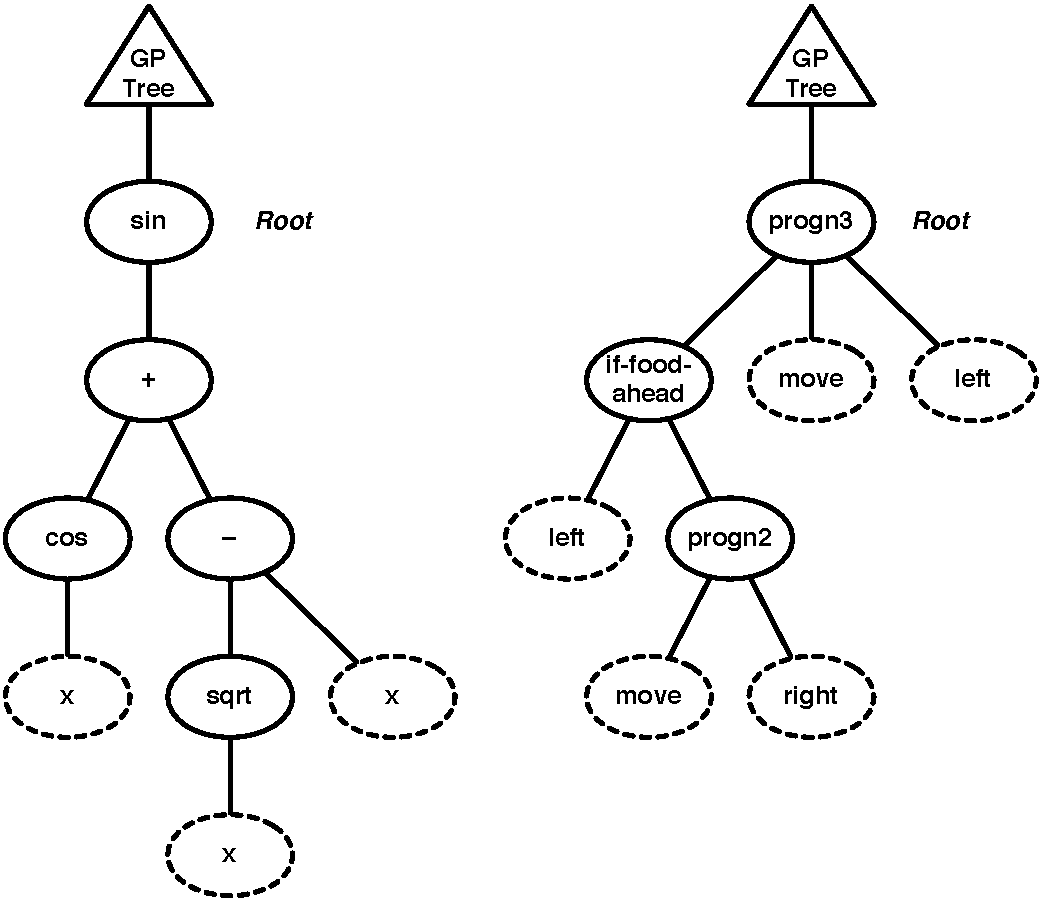
\includegraphics[width=4in]{gptrees.pdf}
\end{center}
\caption{Two example genetic programming parse trees.  At top is a single \class{ec.gp.GPTree} instance, which holds onto a single \class{ec.gp.GPNode} designated the {\it root} of the tree.  GPNodes form the tree itself, and so have a {\it parent} and zero or more {\it children}.  The parent of the root is the GPTree object itself.  Leaf nodes, denoted with dotted ovals, are traditionally called {\it terminals}, and non-leaf nodes, including the root, are traditionally called {\it nonterminals}.  Normally GPNodes have fixed arity.  That is, all \class{if-food-ahead} GPNodes will always have two children, and all \class{cos} nodes will always have one child, etc.}
\label{gptrees}
\end{figure}


\subsection{GPNodes, GPTrees, and GPIndividuals}

Figure \ref{gptrees} shows two example trees of GPNodes (shown as ovals).  The top of each tree is a GPTree, and directly under it is the {\it root} GPNode.  As can be seen from the figure, each GPNode has both a parent and zero or more children; and each GPTree has exactly one child.  Both GPNodes and GPTrees implement \class{ec.gp.GPNodeParent}, and can serve as parents of other GPNodes (the root has the GPTree as its parent). 

\subsubsection{GPNodes}  A basic GPNode consists of four items:

\java{%
    public GPNodeParent parent;\\
    public GPNode children[];\\
    public byte argposition;\\
    public byte constraints;
}

The \variable{parent} should be self-explanatory.  The \variable{children[]} is an array holding the children to the GPNode.  Leaf nodes in a GP tree (traditionally called {\bf terminals} are permitted to either have a zero-length array or a null value for \variable{children[]}.

The \variable{argposition} is the position of the node in its {\it parent's} \variable{children[]} array.  The root's \variable{argposition} is 0.  Last, the \variable{constraints} is a tag which refers to the GPNode's GPNodeConstraints object.  It's a byte rather than a full pointer to save a bit of space: GPNodes make up by far the bulk of memory in a genetic programming experiment.  You can get the GPNodeConstraints by calling the following GPNode method:

\java{%
    public final GPNodeConstraints constraints(GPInitializer initializer);
}

Why the GPInitializer?  Because GPNodeConstraints, GPTreeConstraints, GPTypes, and GPFunctionSets are all accessible via Initializer, which must be a GPInitializer.\footnote{It wasn't a good decision to use the Initializer in this fashion, and one day we may change it to something else.}  More on that later.  Assuming you have access to the EvolutionState (probably called \variable{state}) can call this function like this:

\java{%
	GPNodeConstraints constraints = myGPNode.constraints((GPInitializer)(state.initializer));
}

You will make various subclasses of GPNode to define the kinds of functions which may appear in your genetic programming tree.

\subsubsection{GPTrees}  Unlike GPNode, which is liberally subclassed, you'll rarely subclass GPTree.  The \class{ec.gp.GPTree} class holds onto the root GPNode here:

\java{%
	public GPNode child;
}

Each GPTree also has a backpointer to the GPIndividual which holds it:

\java{%
	public GPIndividual owner;
}

GPTree also has a pointer to its GPTreeConstraints object.  Like GPNode, GPTree uses a byte rather than a full pointer.\footnote{This is mostly historic: GPTree doesn't fill nearly as much memory as GPNode and so doesn't really need this tight reference approach.} 

\java{%
	public byte constraints;
}

Just like GPNode, you can access GPTree's constraints using this function:

\java{%
    public final GPTreeConstraints constraints(GPInitializer initializer);
}

\noindent ...which is typically called like this:

\java{%
	GPTreeConstraints constraints = myGPTree.constraints((GPInitializer)(state.initializer));
}

\subsubsection{GPIndividual}

The GPIndividual contains an array of GPTrees.  In most cases, this array has a single GPTree in it:

\java{%
    public GPTree[] trees;
}

\subsubsection{GPNodeConstraints}

The GPNodeConstraints contains several data elements shared by various GPNodes:

\java{%
    public byte constraintNumber;\\
    public GPType returntype;\\
    public GPType[] childtypes;\\
    public String name;\\
    public float probabilityOfSelection;\\
    public GPNode zeroChildren[] = new GPNode[0];
}

The first element is obvious: it's number of the constraints which the GPNode objects point to.  The next two items hold the return type and children types of the node: more on that later.  Specifically, the return type of a child in slot 0 must be compatible with the child type declared for slot 0.  For now what matters is that you can determine the expected number of children to a GPNode by the length of the \variable{childtypes} array.

The \variable{name} variable holds the name of the GPNodeConstraints ({\it not} the GPNodes which refer to them): we'll define some in the next section.  The \variable{probabilityOfSelection} variable holds an auxiliary variable used by certain tree-building operators.  Last, \variable{zeroChildren[]} holds a blank, zero-length GPNode which terminals are free to use in lieu of null for their children.

\java{%
    public GPTree[] trees;
}

\subsubsection{GPTreeConstraints}

The GPTreeConstraints contains data elements shared by GPTrees:

\java{%
    public byte constraintNumber;\\
    public GPType treetype;\\
    public String name;\\
    public GPNodeBuilder init;\\
    public GPFunctionSet functionset;
}

The first element is again obvious.  The \variable{treetype} variable declares the GPType for the tree as a whole: the return type of the root must be compatible with this type.  The \variable{name} works similarly to the one in GPNodeConstraints.

The last two variables are critical.  The \variable{init} variable holds the algorithm used to generate trees or subtrees for this GPTree.  We will discuss tree builders later.  Last, the \variable{functionset} variable holds the function set for this tree: all GPNodes appearing in this GPTree must be cloned from this function set.

\subsubsection{GPFunctionSet}

The GPFunctionSet contains a \variable{name} (like GPNodeConstraints and GPTreeConstraints) and a set of GPNodes, clones of which may appear in the GPTree.  This set is stored in various hash tables and arrays to make lookup easy for different common queries (such as ``give me all terminals'') or (``give me all nodes whose return type is {\it foo}'').  Usually you don't need to access this class directly: instead, we'll set up the function set using parameters.


\subsection{Basic Setup}
\label{basicsetup}

Now let's work towards setting a GP problem.  We begin by defining the GPIndividual and GPSpecies.  Usually, we'll just use those classes directly:

\params{%
pop.subpop.0.species = ec.gp.GPSpecies\\
pop.subpop.0.species.ind = ec.gp.GPIndividual
}

Let's presume for now that we just want a single tree per GPIndividual.   This is the usual case.  Typically this class is defined by GPTree unless we're doing something odd.  We say:

\params{%
pop.subpop.0.species.ind.numtrees = 1\\
pop.subpop.0.species.ind.tree.0 = ec.gp.GPTree
}

Different trees can have different GPTreeConstraints objects, or share them.  This is done by defining a set of GPTreeConstraints (which is a Clique, Section~\ref{clique}) and giving each member of the set a unique identifier.  Then GPTrees identify with a given GPTreeConstraints by using that identifier.

Since we have only one tree, we really only need to create one GPTreeConstraints.  We'll call it ``\variable{tc0}''.

\params{%
gp.tc.size = 1\\
gp.tc.0 = ec.gp.GPTreeConstraints\\
gp.tc.0.name = tc0
}

Note that as a Clique, GPTreeConstraints objects all have a global parameter base of \parameter{gp.tc}.  Now we assign it to the tree:

\params{%
pop.subpop.0.species.ind.tree.0.tc = tc0
}

A GPTreeConstraints object in turn holds onto the GPFunctionSet used to construct trees which identify with it.  GPFunctionSet is also a clique.  We'll call the function set ``\variable{f0}'':

\params{%
gp.fs.size = 1\\
gp.fs.0 = ec.gp.GPFunctionSet\\
gp.fs.0.name = f0
}

Note that as a Clique, GPFunctionSet objects all have a global parameter base of \parameter{gp.fs}.  We now assign this function set to our tree constraints:

\params{%
gp.tc.0.fset = f0
}

As to types: we'll discuss typed GP later on.  For now we'll assume that there is a single atomic type which is used universally by everyone\,---\,that is, everything can connect with everything (it's ``typeless'').  This is the classic GP scenario.  GPTypes are also a clique: and they have a global parameter base of \parameter{gp.type}.  We define zero GPSetTypes and one GPAtomicType (which we will name, for lack of a better word, ``\parameter{nil}'') like this:

\params{%
gp.type.a.size = 1\\
gp.type.a.0.name = nil\\
gp.type.s.size = 0
}

Our GPTreeConstraints object needs to define the GPType of the tree as a whole (the ``root type'').  To se it to our \parameter{nil} type, we'd say:

\params{%
gp.tc.0.returns = nil\\
}

Last, we need to define some GPNodeConstraints.  A GPNodeConstraint object describes three things about the GPNodes related to them via the Flyweight pattern:

\begin{itemize}
\item The number of children of the GPNode.
\item The GPTypes that the children of the GPNode must be consistent with.
\item The GPType of that the parent of the GPNode must be consistent with.
\end{itemize}

More on types later.  But for now we'll define a few GPNodeConstraints for nodes with zero, one, and two children.  Since we only have one type, the types of all the children and the parent are all going to be \parameter{nil}.  We'll call these GPNodeConstraints \parameter{nc0}, \parameter{nc1}, and \parameter{nc2}.

\params{%
gp.nc.size = 3\\
\\
gp.nc.0 = ec.gp.GPNodeConstraints\\
gp.nc.0.name = nc0\\
gp.nc.0.returns = nil\\
gp.nc.0.size = 0\\
\\
gp.nc.1 = ec.gp.GPNodeConstraints\\
gp.nc.1.name = nc1\\\
gp.nc.1.returns = nil\\
gp.nc.1.size = 1\\
gp.nc.1.child.0 = nil\\
\\
gp.nc.2 = ec.gp.GPNodeConstraints\\
gp.nc.2.name = nc2\\
gp.nc.2.returns = nil\\
gp.nc.2.size = 2\\
gp.nc.2.child.0 = nil\\
gp.nc.2.child.1 = nil
}

\subsubsection{Defining GPNodes}
\label{defininggpnodes}

Let's imagine that we're trying to create trees that consist of the following tree nodes (which we'll create later):  \class{ec.app.myapp.X, ec.app.myapp.Y, ec.app.myapp.Mul, ec.app.myapp.Sub, ec.app.myapp.Sin}.  These nodes take 0, 0, 2, 2, and 1 children respectively and have no special types (we'll use \variable{nil}).   We could add them to the function set like this:

\params{%
gp.fs.0 = ec.gp.GPFunctionSet\\
gp.fs.0.size = 5\\
gp.fs.0.func.0 = ec.app.myapp.X\\
gp.fs.0.func.0.nc = nc0\\
gp.fs.0.func.1 = ec.app.myapp.Y\\
gp.fs.0.func.1.nc = nc0\\
gp.fs.0.func.2 = ec.app.myapp.Mul\\
gp.fs.0.func.2.nc = nc2\\
gp.fs.0.func.3 = ec.app.myapp.Sub\\
gp.fs.0.func.3.nc = nc2\\
gp.fs.0.func.4 = ec.app.myapp.Sin\\
gp.fs.0.func.4.nc = nc1
}

Notice that we don't state the number of children or the types explicitly: instead we state them implicitly by assigning the appropriate GPNodeConstraints object.



\subsection{Defining the Representation, Problem, and Statistics}
\label{definingtherepresentation}

GP is more complex than most other optimization procedures because of its representation.  When you create a GP problem, you have two primary tasks:

\begin{itemize}
\item Create the GPNodes with which a GPIndividual may be constructed
\item Create a Problem which tests the GPIndividual
\end{itemize}

Let's start with the first one.  As an example, we'll build a simple Symbolic Regression example on two variables, X and Y.  The GP tree can have GPNodes which subtract, multiply, and perform sine, just as was done earlier.  \footnote{Ridiculously limited, but what did you expect?  This is a demonstration example!}  This means we'll need two terminals (X and Y), and three nonterminals (subtract and multiply, each of arity 2\,---\,two children each\,---\, and cosine, with arity 1).

Recall from Section~\ref{basicsetup} that our function set would look like this:

\params{%
gp.fs.0 = ec.gp.GPFunctionSet\\
gp.fs.0.size = 5\\
gp.fs.0.func.0 = ec.app.myapp.X\\
gp.fs.0.func.0.nc = nc0\\
gp.fs.0.func.1 = ec.app.myapp.Y\\
gp.fs.0.func.1.nc = nc0\\
gp.fs.0.func.2 = ec.app.myapp.Mul\\
gp.fs.0.func.2.nc = nc2\\
gp.fs.0.func.3 = ec.app.myapp.Sub\\
gp.fs.0.func.3.nc = nc2\\
gp.fs.0.func.4 = ec.app.myapp.Sin\\
gp.fs.0.func.4.nc = nc1
}

We need to make each of these classes.  Each of these are GPNodes with a single crucial method overridden:

\java{%
    public abstract void eval(EvolutionState state,
        int thread,
        GPData input,\\
\hsp{\fill}ADFStack stack,
        GPIndividual individual,
        Problem problem);
}

\begin{figure}[t]
\begin{center}
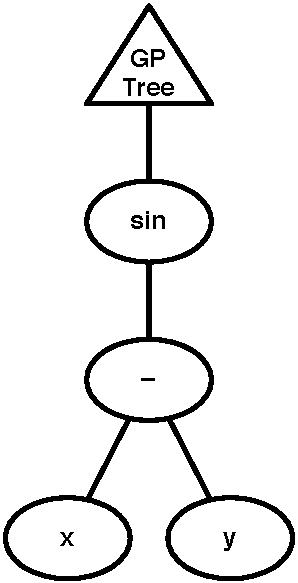
\includegraphics[width=1.1in]{simplegptree.pdf}
\end{center}
\caption{A simple GP tree representing the mathematical expression \(\sin(x-y)\).}
\label{simplegptree}
\end{figure}

This method is called when the GPNode is being executed in the course of executing the tree.  Execution proceeds depth-first like the evaluation of a standard parse tree.  For example, in order to compute the expression \(\sin(x - y)\) (shown in GP form in Figure \ref{simplegptree}) we will call \method{eval(...)} on the Sin object, which will in turn call \method{eval(...)} on the Sub object.  This will then call \method{eval(...)} on the X object, then on the Y object.  X and Y will return their values.  The Sub object will then subtract them and return the result, and finally Sin will return the sine of that.

Execution doesn't have to be just in terms of calling \method{eval(...)} on children, processing the results, and returning a final value.  In fact, for some problems the return value may not matter at all, but simply which nodes are executed.  In this case, likely the nodes themselves are doing things via side effects: moving a robot around, for example.  Execution could also be tentative: an ``if'' node might evaluate one or another of its children and leave it at that.  Execution could also be repetitive: you might make a ``while'' node which repeatedly evaluates a child until some test is true.  Basically you can execute these nodes any way that might appear in a regular programming language.

\subsubsection{GPData} 
\label{ec.gp.GPData}

The \method{eval(...)} method has several arguments, only two of which should be nonobvious: \class{ec.gp.ADFStack}  and \class{ec.gp.GPData}.  We will discuss ADFStack later in Section~\ref{ec.gp.ADF}.  The GPData object is a simple data object passed around amongst your GPNodes when they execute one another.  It's your opportunity to pass data from node to node. In the example above, it's how the values are passed from the children to their parents: for example, it's how the Sub node returns its value to the Sin node.  It's also possible that the parent needs to pass data to its child: and the GPData object can be used like that as well.

Typically a single GPData object is created and handed to the GPNodes, and then they hand it to one another during execution, reusing it. This avoids making lots of clones of a GPData object during execution.

Our GPData object needs to hold the return value from a child.  If you are holding a simple piece of data (like a double or an int) also just need to implement a single method, \method{copyTo(...)}, which copies the data from your GPData object into another, then returns it:

\java{%
public abstract GPData copyTo(GPData other);
}

In this case, it's simple:

\vbox{\small
\begin{verbatim}
package ec.app.myapp;
import ec.gp.*;
public class MyData extends GPData
    {
    public double val;
    public void copyTo(GPData other)
        { ((MyData)other).val = val;  return other;  }
    }
\end{verbatim}
}

Now it might be the case that you need to hold more complex data.  For example, what if you had an array of doubles?  In this case you'd need to either clone or copy the data during the \method{copyTo(...)} operation.  Additionally, GPData is a Prototype and so it needs to implement the \method{clone()} method as a deep clone.  The default implementation just does a light clone.  But with your array of doubles, you'd need to clone that.  Altogether you might have something like this:

\vbox{\small
\begin{verbatim}
package ec.app.myapp;
import ec.gp.*;
public class MyData extends GPData
    {
    public double[15] val = new double[15];
    public void copyTo(GPData other)
        {
        System.arraycopy(val, 0, ((MyData)other).val, 0, val.length);
        return other;  
        }

    public Object clone()
        {
        MyData other = (MyData)(super.clone());
        other.val = (double[])(val.clone());
        return other;  
        }
    }
\end{verbatim}
}

The important thing to note is that when you perform \method{copyTo(...)} or \method{clone()}, the resulting other object should not be sharing any data in common with you except constant (immutable, read-only) data.  Why the two methods?  Certainly most things \method{copyTo(...)} performs could be done with \method{clone()}.  The reason for \method{copyTo(...)} is entirely for efficiency when using Automatically Defined Functions (Section~\ref{ec.gp.ADF}).  Perhaps in the future we might obviate the need for its use.


\subsubsection{KozaFitness}

You can use any fitness you like for GP.  But it's common to use a particular fitness function popularized by John Koza \cite{koza:book}.  This fitness object contains a {\it standardized fitness} in which 0 is the ideal result and Infinity is worse than the worst possible result.  Note that this isn't yet the correct fitness according the \class{ec.Fitness}.  Instead, when asked for fitness, the function converts this to an {\it adjusted fitness} in which 1 is the ideal result and 0 is worse than the worst possible result, using the function \(\frac{1}{1 + \text{standardized}}\).  The adjusted fitness makes this a valid Fitness subclass.  The GP fitness also has an auxiliary variable, \variable{hits}, which originally was meant to indicate how many optimal subsolutions were discovered: it's printed out in the statistics and used for nothing else; use it as you like.  This fitness is set as:

\params{%
pop.subpop.0.species.fitness = ec.gp.koza.KozaFitness
}

The standard fitness-setting function for this class is:

\java{%
public final void setStandardizedFitness(EvolutionState state, float value);
}

You can get (or set) the hits as:

\java{%
int hits = myKozaFitness.hits;
}


\subsubsection{GPProblem} 

With all that out of our hair, let's construct the Problem.  Let's attempt to create a GP tree which closely matches a set of data we've created: we'll generate the data from the function \(z = \sin(x \times y) - \sin(x) - x \times y\), in the range \([0,1)\) for both \(x\) and \(y\).  What we'll do is define \(n\) \(\langle x, y\rangle\) data points up front, then evaluate our individuals.  For each data point, we'll set some global variables accessible by the X and Y GPNodes.  The individual will return a value, which we'll compare against the expected \(z\) result.  The fitness will be the sum of squared differences.

{\small
\begin{verbatim}
package ec.app.myapp;
import ec.gp.*;
import ec.simple.*;
import ec.*;
import ec.gp.koza.*;
public class MyProblem extends GPProblem implements SimpleProblemForm {
    final static int N = 20;
    int current;
    double[] Xs = new double[N];  // will be pointer-copied in clone(), which is okay
    double[] Ys = new double[N]; // likewise
    double[] Zs = new double[N]; // likewise
    MyData data;
	
    public void setup(EvolutionState state, Parameter base) {
        super.setup(state, base);

        // generate N random <x, y, z = f(x,y)> tuples
        for(int i = 0; i < N; i++) {
            double x, y;
            Xs[i] = x = state.random[0].nextDouble();
            Ys[i] = y = state.random[0].nextDouble();
            Zs[i] = Math.sin(x * y) - Math.sin(x) - x * y;
            }
	
        // create a GPData object
        data = (MyData) state.parameters.getInstanceForParameterEq(base.push(P_DATA),
            null, MyData.class);
        data.setup(state, base.push(P_DATA));
        }
	
    public Object clone()    // we'll clone the GPData so each thread has its own copy
        {
        MyProblem obj = (MyProblem)(super.clone());
        obj.data = (MyData)(data.clone());
        return obj;
        }

    public void evaluate(final EvolutionState state,  Individual ind, 
        int subpopulation, int threadnum) {
        if (!ind.evaluated) {    // don't bother reevaluating
            double sum = 0.0;
            
            // for each tuple, evaluate the individual.  For good measure reset
            // the GPData first, though in this example it's not necessary
            data.val = 0;
            for(current = 0; current < N; current++)    // note: an instance variable
                ((GPIndividual)ind).trees[0].child.eval(
                    state, threadnum, data, stack, ((GPIndividual)ind),this);
            sum += (data.val * data.val);
            
            // set the fitness and the evaluated flag
            KozaFitness f = (KozaFitness)(ind.fitness);
            f.setStandardizedFitness(state, sum);
            f.hits = 0;  // don't bother using this
            ind.evaluated = true;
            }
        }
    }
\end{verbatim}
}

\subsubsection{GPNode Subclasses}

Now let's implement our five GPNode subclasses.  Each will implement \method{toString()} to print out the node name, and also \method{eval(...)} discussed earlier.  It's also common to implement the method \method{checkConstraints()} to do a final sanity-check on the node (whether it has the right number of children, etc.) but it's not necessary, and we'll omit it here.

First the terminals:

\vbox{\small
\begin{verbatim}
package ec.app.myapp;
import ec.*;
import ec.gp.*;
public class X extends GPNode {
    public String toString() { return "x" };
    public void eval(EvolutionState state, int thread, GPData input,
              ADFStack stack, GPIndividual indivdiual, GPProblem problem) {
        MyData data = (MyData) input;
        MyProblem prob = (MyProblem) problem;
        
        data.val = problem.Xs[problem.current];  // return current X value to parent
        }
    }
\end{verbatim}
}

\noindent ... and...

\vbox{\small\begin{verbatim}
package ec.app.myapp;
import ec.*;
import ec.gp.*;
public class Y extends GPNode {
    public String toString() { return "y" };
    public void eval(EvolutionState state, int thread, GPData input,
              ADFStack stack, GPIndividual indivdiual, GPProblem problem) {
        MyData data = (MyData) input;
        MyProblem prob = (MyProblem) problem;
        
        data.val = problem.Ys[problem.current];  // return current Y value to parent
        }
}
\end{verbatim}
}
Next the Sine:

\vbox{\small\begin{verbatim}
package ec.app.myapp;
import ec.*;
import ec.gp.*;
public class Sin extends GPNode {
    public String toString() { return "sin" };
    public void eval(EvolutionState state, int thread, GPData input,
              ADFStack stack, GPIndividual indivdiual, GPProblem problem) {
        MyData data = (MyData) input;
        MyProblem prob = (MyProblem) problem;
        
        children[0].eval(state, thread, data, stack, individual, prob);
        data.val = Math.sin(data.val);
        }
    }
\end{verbatim}
}

Next the Multiply and Subtract:

\vbox{\small\begin{verbatim}
package ec.app.myapp;
import ec.*;
import ec.gp.*;
public class Mul extends GPNode {
    public String toString() { return "*" };
    public void eval(EvolutionState state, int thread, GPData input,
              ADFStack stack, GPIndividual indivdiual, GPProblem problem) {
        MyData data = (MyData) input;
        MyProblem prob = (MyProblem) problem;
        
        children[0].eval(state, thread, data, stack, individual, prob);
        double val1 = data.val;
        
        children[1].eval(state, thread, data, stack, individual, prob);
        data.val = val1 * data.val;
        }
    }
\end{verbatim}
}

\vbox{\small\begin{verbatim}
package ec.app.myapp;
import ec.*;
import ec.gp.*;
public class Sub extends GPNode {
    public String toString() { return "-" };
    public void eval(EvolutionState state, int thread, GPData input,
              ADFStack stack, GPIndividual indivdiual, GPProblem problem) {
        MyData data = (MyData) input;
        MyProblem prob = (MyProblem) problem;
        
        children[0].eval(state, thread, data, stack, individual, prob);
        double val1 = data.val;
        
        children[1].eval(state, thread, data, stack, individual, prob);
        data.val = val1 - data.val;
        }
    }
\end{verbatim}
}
\subsubsection{Statistics}

The default statistics class for GP is SimpleStatistics.  However, the GP package has a Statistics subclass  designed for doing the same basic stuff as SimpleShortStatistics, but with some extra GP-specific tree statistics.  You can turn it on like this:

\params{%
stat = ec.gp.koza.KozaShortStatistics
}

In this form, once a generation the statistics will print out a line consisting of the following items (space-delimited):

\begin{enumerate}
\item The generation number
\item {\it Once for each subpopulation...}
\begin{enumerate}
	\item The mean standardized fitness of the subpopulation for this generation
	\item The mean adjusted fitness of the subpopulation for this generation
	\item The mean hits of the subpopulation for this generation
	\item The best standardized fitness of the subpopulation for this generation
	\item The best adjusted fitness of the subpopulation for this generation
	\item The best hits of the subpopulation for this generation
	\item The best standardized fitness of the subpopulation so far in the run
	\item The best adjusted fitness of the subpopulation so far in the run
	\item The best hits of the subpopulation so far in the run
\end{enumerate}
\end{enumerate}

For example, we might have values like this...

\script{%
0 85.52637 0.011589747 3.4736328125 64.0 0.015384615 25 64.0 0.015384615 25 \\
1 81.93652 0.0121164825 7.0634765625 59.0 0.016666668 30 59.0 0.016666668 30 \\
2 78.8916 0.012612895 10.1083984375 53.0 0.018518519 36 53.0 0.018518519 36 \\
3 76.83887 0.012973738 12.1611328125 55.0 0.017857144 34 53.0 0.018518519 36 \\
4 74.421875 0.013421775 14.578125 51.0 0.01923077 38 51.0 0.01923077 38 \\
5 71.825195 0.013957807 17.1748046875 49.0 0.02 40 49.0 0.02 40 
}

KozaShortStatistics has an option for including more statistics.  If we turned on the following parameter:

\params{%
stat.child.0.gather-full = true
}

...we'd have the following values printed out:


\begin{enumerate}
\item The generation number
\item How long initialization took in milliseconds (for generation 0), or how long the previous generation took to breed to form this generation (for generations \(>0\)).
\item How many bytes initialization took (for generation 0), or how many bytes the previous generation took to breed to form this generation (for generations \(>0\)).  This is an approximation and in some cases might even be negative due to garbage collection.
\item How long evaluation took in milliseconds for this generation.
\item How many bytes evaluation took for this generation.    This is an approximation and in some cases might even be negative due to garbage collection.
\item {\it Once for each subpopulation...}
\begin{enumerate}
	\item The average number of GPNodes used per individual this generation (its size)
	\item In the form [a{\textbar}b{\textbar}c...], the average number of GPNodes used for the first tree (a), second tree (b), third tree (c), etc., of individuals this generation.	
	\item The average number of GPNodes used per individual so far in the run
	\item The average depth of any tree per individual this generation
	\item In the form [a{\textbar}b{\textbar}c...], the average depth of the first tree (a), second tree (b), third tree (c), etc., of individuals this generation.	
	\item The average depth of any tree per individual so far in the run
	\item The mean standardized fitness of the subpopulation for this generation
	\item The mean adjusted fitness of the subpopulation for this generation
	\item The mean hits of the subpopulation for this generation
	\item The best standardized fitness of the subpopulation for this generation
	\item The best adjusted fitness of the subpopulation for this generation
	\item The best hits of the subpopulation for this generation
	\item The best standardized fitness of the subpopulation so far in the run
	\item The best adjusted fitness of the subpopulation so far in the run
	\item The best hits of the subpopulation so far in the run
\end{enumerate}
\end{enumerate}

It'd look something like this (made tiny to fit one to a line):

{\tiny\begin{verbatim}0 27 -241424 0 0 34.1 [8.9|18.2|7.0] 34.1 3.3 [4.1|2.9|2.9] 9.9 60.0 0.016445229 4.0 53.0 0.018518519 11 53.0 0.018518519 11
1 1 9680 0 0 36.5 [14.0|15.0|7.5] 35.3 3.9 [5.8|2.8|3.1] 10.8 56.2 0.017573431 7.8 49.0 0.02 15 49.0 0.02 15
2 0 9680 1 0 28.7 [15.6|3.0|10.1] 33.1 3.966666666666667 [6.3|2.0|3.6] 11.166666666666666 50.4 0.019522537 13.6 46.0 0.021276595 18 46.0 0.021276595 18
3 1 19352 1 0 39.5 [17.3|3.0|19.2] 34.7 4.666666666666667 [6.6|2.0|5.4] 11.875 47.1 0.02080979 16.9 45.0 0.02173913 19 45.0 0.02173913 19
4 1 19368 1 0 40.9 [18.6|3.0|19.3] 35.94 4.8 [7.0|2.0|5.4] 12.38 46.2 0.021393415 17.8 40.0 0.024390243 24 40.0 0.024390243 24 
\end{verbatim}
}


\subsection{Initialization}

To use GP we'll need to define the initializer as a subclass of \class{ec.gp.GPInitializer}:

\params{%
init = ec.gp.GPInitializer
}

ECJ has traditionally followed the {\it lil-gp} default for disallowing duplicates in the initial Population: if a duplicate is created, ECJ will try 100 times to create another non-duplicate Individual in its stead.  If this fails, the last duplicate created will be allowed.  We say this in the standard way:

\params{%
pop.subpop.0.duplicate-retries = 100
}

To create trees. ECJ relies on a tree-creation algorithm in the form of an \class{ec.gp.GPNodeBuilder}, part of the GPTreeConstraints object.  The GPNodeBuilder for GPTreeConstraints 0 is specified like this:

\params{%
gp.tc.0.init = ec.gp.koza.HalfBuilder
}

ECJ provides quite a number of node builders in the \package{ec.gp.koza} and \package{ec.gp.build} packages.  You request a tree with the following function:

\java{%
public abstract GPNode newRootedTree(EvolutionState state, GPType type,\\
\hsp{\fill}int thread, GPNodeParent parent, GPFunctionSet set,\\
\hsp{\fill}int argposition, int requestedSize);
}

This method builds a tree of GPNodes whose root return type is compatible with \variable{type}, attached to the given \variable{GPNodeParent}, at position \variable{argposition}, and built from clones of GPNodes in the function set \variable{set}.  The root node is returned.  Several GPNodeBuilders also produce the tree of the \variable{requestedSize}: others ignore this function.  You can also ask the GPNodeBuilder to pick its own tree size from a distribution specified by the user in parameters, by passing \variable{ec.gp.GPNodeBuilder.NOSIZEGIVEN} for the size (this is the usual thing done by most initialization procedures).

If you are using a GPNodeBuilder which generates trees of a certain size, and \variable{ec.gp.GPNodeBuilder.NOSIZEGIVEN} is used (as usual), then you can specify a distribution of sizes in two ways.  First, you can have the GPNodeBuilder pick a size uniformly from among a minimum and maximum size, for example:

\params{%
gp.tc.0.init.min-size = 10\\
gp.tc.0.init.max-size = 20
}

Alternatively you can specify the distribution of sizes manually.  To stipulate probabilities sizes for 1, 2, 3, 4, and 5, you'd say:

\params{%
gp.tc.0.init.num-sizes = 5\\
gp.tc.0.init.size.0 = 0.2\\
gp.tc.0.init.size.1 = 0.1\\
gp.tc.0.init.size.2 = 0.2\\
gp.tc.0.init.size.3 = 0.25\\
gp.tc.0.init.size.4 = 0.25
}


ECJ has a whole bunch of GPNodeBuilder algorithms available to you.  I wrote a shoot-out paper describing and comparing nearly all of these algorithms \cite{Luke1:2001:GECCO}.  Here is the run-down:

\begin{itemize}

\item \class{ec.gp.koza.FullBuilder} generates full trees using Koza's FULL algorithm.  You cannot request a size.  It requires a minimum and maximum depth, for example:

\params{%
gp.tc.0.init = ec.gp.koza.FullBuilder\\
gp.tc.0.init.min-depth = 2\\
gp.tc.0.init.max-depth = 6
}

Alternatively:

\params{%
gp.koza.full.min-depth = 2\\
gp.koza.full.max-depth = 6
}

\item \class{ec.gp.koza.GrowBuilder} generates arbitrary trees depth-first using Koza's GROW algorithm. You cannot request a size. It requires a minimum and maximum depth, for example:

\params{%
gp.tc.0.init = ec.gp.koza.GrowBuilder\\
gp.tc.0.init.min-depth = 2\\
gp.tc.0.init.max-depth = 6
}

Alternatively:

\params{%
gp.koza.grow.min-depth = 2\\
gp.koza.grow.max-depth = 6
}

\item \class{ec.gp.koza.HalfBuilder} generates arbitrary trees depth-first using Koza's RAMPED HALF-AND-HALF algorithm.  You cannot request a size. This is nothing more than flipping a coin to decide whether to use GROW or FULL.  HalfBuilder is the default builder for creating GP trees in ECJ, but it's not particularly good.  It requires a minimum and maximum depth, and the probability of doing GROW, for example:

\params{%
gp.tc.0.init = ec.gp.koza.HalfBuilder\\
gp.tc.0.init.min-depth = 2\\
gp.tc.0.init.max-depth = 6\\
gp.tc.0.init.growp = 0.5
}

Alternatively:

\params{%
gp.koza.half.min-depth = 2\\
gp.koza.half.max-depth = 6\\
gp.koza.half.growp = 0.5
}

\item \class{ec.gp.build.PTC1} is a modification of GROW which guarantees that trees will be generated with a given mean.  You cannot request a size. Additionally, each terminal and nonterminal can specify its probability of being chosen from the function set as PTC1 constructs the tree.  PTC1 requires an expected size and a maximum depth:

\params{%
gp.tc.0.init = ec.gp.build.PTC1\\
gp.tc.0.init.expected-size = 10\\
gp.tc.0.init.max-depth = 6
}

Alternatively:

\params{%
gp.build.ptc1.expected-size = 10\\
gp.build.ptc1.max-depth = 6
}

PTC1 requires that its function sets adhere to the interface \class{ec.gp.build.PTCFunctionSetForm}.  This interface contains three tables of probabilities for your GPNodes to be selected:

\java{%
    public float[] terminalProbabilities(int type);\\
    public float[] nonterminalProbabilities(int type);\\
    public float[] nonterminalSelectionProbabilities(int expectedTreeSize);
}

The first function returns, for a given GPType number, a distribution of desired selection probabilities for terminals of that type.  The order of the terminals is the same as the following array in GPFunctionSet:

\java{%
    public GPNode[type][] terminals;
}

The second function returns, for a given GPType number, a distribution of desired selection probabilities for nonterminals of that type.  The order of the nonterminals is the same as the following array in GPFunctionSet:

\java{%
    public GPNode[type][] nonterminals;
}

The final function returns, for a given desired tree size, the probability that a nonterminal (of a given GPType return type) should be selected over a terminal of the same GPType.  This is only used by PTC1, not PTC2 below.

You don't need to implement this interface: the \class{ec.gp.build.PTCFunctionSet} class does it for you:

\params{%
gp.fs.size = 1\\
gp.fs.0 = ec.gp.build.PTCFunctionSet\\
gp.fs.0.name = f0
}

This function set computes all the above probabilities from user-specified probabilities as parameters.  The probabilities are specified by each GPNodeConstraints object.  Following the example we started in Section~\ref{basicsetup}, we might state that the terminals X and Y (node constraints 0) should be picked with 0.5 probability each, and the nonterminals Mul, Sub (node constraints 2) and Cos (node constraints 1) should be picked with 0.3, 0.3, and 0.4 probability:

\params{%
gp.nc.0.prob = 0.5\\
gp.nc.1.prob = 0.3\\
gp.nc.2.prob = 0.4
}

What if you wanted Mul and Sub to have different probabilities?  You'd need to create different GPNodeConstraints.  For example, we could create a new, separate GPNodeConstraints for Sub:

\params{%
gp.nc.size = 4\\
gp.nc.3 = ec.gp.GPNodeConstraints\\
gp.nc.3.name = nc3\\
gp.nc.3.returns = nil\\
gp.nc.3.size = 2\\
gp.nc.3.child.0 = nil\\
gp.nc.3.child.1 = nil
}

Now we assign it to Sub:

\params{%
gp.fs.0.func.3 = ec.app.myapp.Sub\\
gp.fs.0.func.3.nc = nc3
}

\noindent ...and last change the probabilities of Sub and Mul to be different:

\params{%
gp.nc.0.prob = 0.5\\
gp.nc.1.prob = 0.3\\
gp.nc.2.prob = 0.25\\
gp.nc.3.prob = 0.35
}



\item \class{ec.gp.build.PTC2} generates trees near to a desired size (which you request) by picking randomly from the current outer edge in the tree and adding a node.  When the tree is large enough, all the remaining edge slots are filled with terminals.  Additionally, each terminal and nonterminal can specify its probability of being chosen from the function set as PTC2 constructs the tree.  PTC2 requires a desired size and a maximum depth:

\params{%
gp.tc.0.init = ec.gp.build.PTC2\\
gp.tc.0.init.expected-size = 10\\
gp.tc.0.init.max-depth = 6
}

Alternatively:

\params{%
gp.build.ptc2.expected-size = 10\\
gp.build.ptc2.max-depth = 6
}

Like PTC1, PTC2 requires that function sets adhere to the PTCFunctionSetForm interface.  Just use PTCFunctionSet.

\item \class{ec.gp.build.RandomBranch} generates trees near to a desired size (which you request) using the RANDOMBRANCH algorithm.  Beyond the size distributions, this algorithm has no additional parameters.

\item \class{ec.gp.build.Uniform} generates trees near to a desired size (which you request) using the UNIFORM algorithm, which selects trees of any tree size.  You can select sizes either using the user distribution, or according to the natural distribution of tree sizes.  To do the second, you'd say:

\params{%
gp.tc.0.init = ec.gp.build.Uniform\\
gp.tc.0.init.true-dist = true
}

Alternatively:

\params{%
gp.breed.uniform.true-dist = true
}

{\bf WARNING:} This algorithm is complex and I fear it may be suffering from bit-rot.  I have been told it's not working properly any more but have not debugged it yet.  

\item \class{ec.gp.build.RandTree} (by Alexander Chircop) generates trees near to a desired size (which you request) using the RAND\_TREE algorithm, which selects trees distributed uniformly using Dyck words.  No extra parameters are needed beyond the tree size selection.  {\bf WARNING:} I suspect this algorithm may have some bugs.

\end{itemize}

\subsection{Breeding}
\label{gpbreeding}

ECJ has a large number of breeding pipeline operators for GP trees.  This includes the most common operators used in GP (\class{ec.gp.koza.Crossover}, \class{ec.gp.koza.Mutation}), and several more found in the \package{ec.gp.breed} package.

Pipelines generally pick a single GPTree in a given GPindividual in which to do mutation or crossover.  In most cases you can lock down the specific GPTree, or let the pipeline choose it at random.

Once they've picked a GPTree, GP breeding operators often need to choose GPNodes in the tree in which to perform crossover, mutation, etc.  To do this, they make use of a \class{ec.gp.GPNodeSelector}.  A GPNodeSelector is a simple interface for picking nodes, consisting of the following methods:

\java{%
    public abstract void reset();\\
    public abstract GPNode pickNode(EvolutionState s,
        int subpopulation,\\
\hsp{\fill}int thread,
        GPIndividual ind,
        GPTree tree);
}

When a breeding pipeline needs to pick a node in a particular GPTree of a particular GPIndividual, it first will call the \method{reset()} to get the GPNodeSelector to ready itself, then it will call \method{pickNode(...)} to select a node.  If the breeding pipeline needs another node in the same tree, it can call \method{pickNode(...)} again as many times as necessary.

The standard GPNodeSelector is \parameter{ec.gp.koza.KozaNodeSelector}, which picks certain kinds of nodes with different probabilities.  The kinds of nodes you can state probabilities for are: the root, nonterminals, terminals, and all nodes.  The most common settings are (here as default parameters):

\params{%
gp.koza.ns.terminals = 0.1\\
gp.koza.ns.nonterminals = 0.9\\
gp.koza.ns.root = 0.0
}

This says to pick terminals 10\% of the time, nonterminals 90\% of the time, the root (specifically) 0\% of the time and any arbitrary node 0\% of the time.  The arbitrary-node percentage is whatever is left over from the other three percentages.  (The root could still be picked, since it's a nonterminal or a terminal\,---\,but it won't be {\it specially} picked).

Why might the breeding pipeline need to call \method{pickNode(...)} repeatedly?  Most likely because the chosen GPNode has type constraint problems.  For example, in order to do crossover between the subtrees rooted by two GPNodes, the nodes need to be type-compatible with one another's parent nodes: otherwise the tree locations wouldn't be valid.  Pipelines with these issues will try some \(n\) times to pick compatible nodes; if they fail all \(n\) times, the parents are returned rather than the generated children.

Here are the breeding pipelines that come with ECJ.  In each case, let's presume that we're placing the pipeline as the root pipeline of Subpopulation 0, parameter-wise:

\begin{itemize}

\item \class{ec.gp.koza.CrossoverPipeline} performs standard subtree crossover: it requests a GPIndividual from each of its two sources; then a tree is selected from each GPndividual, then a node is selected in each tree, and finally the two subtrees rooted by those nodes are swapped.  CrossoverPipeline has several parameters.  The first three:

\params{%
pop.subpop.0.species.pipe.tries = 1\\
pop.subpop.0.species.pipe.maxdepth = 17\\
pop.subpop.0.species.pipe.toss = false
}

This tells CrossoverPipeline that children may not have a depth which exceeds 17 (the common value).  The pipeline will to try just one times to find type-valid and depth-legal crossover points before giving up and just returning the parents instead.  This is the most common setting in Genetic Programming.  If \parameter{toss=true} then only one child is returned\,---\,the other is thrown away.  The default value for \parameter{toss} is false.

\params{%
pop.subpop.0.species.pipe.tree.0 = 0\\
pop.subpop.0.species.pipe.tree.1 = 0
}

This tells CrossoverPipeline that it should pick GPNodes in GPTree 0 of each individual.  If either of these parameters is missing entirely, then CrossoverPipeline will pick that tree at random.  At any rate, the GPTrees chosen must have the same GPTreeConstraints.  Finally we have:

\params{%
pop.subpop.0.species.pipe.ns.0 = ec.gp.koza.KozaNodeSelector\\
pop.subpop.0.species.pipe.ns.1 = same
}

This states that the GPNodeSelector for both GPIndividuals should be a KozaNodeSelector.  You can state them independently or node selector 1 can be \parameter{same}.

The default parameter base versions for all of these would be:

\params{%
gp.koza.xover.tries = 1\\
gp.koza.xover.maxdepth = 17\\
gp.koza.xover.toss = false\\
gp.koza.xover.tree.0\\
gp.koza.xover.tree.1\\
gp.koza.xover.ns = ec.gp.koza.KozaNodeSelector
}

{\bf Important note:} the default version of the parameter for node selectors is just \parameter{ns}.  There's no \parameter{ns.0} or \parameter{ns.1}.

\item \class{ec.gp.koza.MutationPipeline} performs standard subtree mutation: it requests a GPIndividual from a single source; then a tree is selected; then a node is selected in that tree; and finally the subtree rooted by that node is replaced in its entirety by a randomly-generated tree.

MutationPipeline has many parameters similar to CrossoverPipeline:

\params{%
pop.subpop.0.species.pipe.tries = 1\\
pop.subpop.0.species.pipe.maxdepth = 17\\
pop.subpop.0.species.pipe.tree.0 = 0\\
pop.subpop.0.species.pipe.ns = ec.gp.koza.KozaNodeSelector
}

Note that the node selector is just \parameter{ns}, not \parameter{ns.0}.

The replacing subtree is generated using a GPNodeBuilder.  The standard GPNodeBuilder is a GrowBuilder with the following default values:

\params{%
gp.koza.grow.min-depth = 5\\
gp.koza.grow.max-depth = 5
}

These are strange default values, but that's common GP original settings.  You stipulate the GPNodeBuilder as:

\params{%
pop.subpop.0.species.pipe.build.0 = ec.gp.koza.GrowBuilder
}

Though GrowBuilder ignores size demands, if you replaced with another builder such as PTC2, you can also optionally stipulate that the replacing subtree must be about the same size as the original subtree.  Here's the parameter:

\params{%
pop.subpop.0.species.pipe.equal = true
}

The default setting is false.

The default parameter base versions for all of these would be:

\params{%
gp.koza.mutate.tries = 1\\
gp.koza.mutate.maxdepth = 17\\
gp.koza.mutate.tree.0 = 0\\
gp.koza.mutate.pipe.ns = ec.gp.koza.KozaNodeSelector\\
gp.koza.mutate.build.0 = ec.gp.koza.GrowBuilder\\
gp.koza.mutate.equal = true
}




\item \class{ec.gp.breed.InternalCrossoverPipeline} selects two GPNodes in the same GPIndividual, such that neither GPNode is in the subtree rooted by the other.  The GPNodes may be in different GPTrees, or they may be in the same GPTree.  It then swaps the two subtrees.

InternalCrossoverPipeline's parameters are essentially identical to those in CrossoverPipeline.  For example:

\params{%
pop.subpop.0.species.pipe.tries = 1\\
pop.subpop.0.species.pipe.maxdepth = 17\\
pop.subpop.0.species.pipe.tree.0 = 0\\
pop.subpop.0.species.pipe.tree.1 = 0\\
pop.subpop.0.species.pipe.ns.0 = ec.gp.koza.KozaNodeSelector\\
pop.subpop.0.species.pipe.ns.1 = same
}

The default parameter base versions for all of these would be:

\params{%
gp.breed.internal-xover.tries = 1\\
gp.breed.internal-xover.maxdepth = 17\\
gp.breed.internal-xover.toss = false\\
gp.breed.internal-xover.tree.0\\
gp.breed.internal-xover.tree.1\\
gp.breed.internal-xover.ns = ec.gp.koza.KozaNodeSelector
}

{\bf Important note:} just as is the case for CrossoverPipeline, the default version of the parameter for node selectors is just \parameter{ns}.  There's no \parameter{ns.0} or \parameter{ns.1}.


\item \class{ec.gp.breed.MutatePromotePipeline} selects a GPNode, other than the root, and replaces its parent (and its parent's subtree) with the GPNode and its subtree.  This was called the {\it PromoteNode} algorithm in \cite{chellapilla:1998:piempwsx} and is similar to the {\it Deletion} algorithm in \cite{OReilly:thesis}.

MutatePromotePipeline's parameters are pretty simple.  Because its constraints are tighter, it doesn't use a GPNodeSelector: instead it searches among all nodes in the tree to find one which is type-compatable with its parent.  thus its parameters are simply the number of times it tries before giving up, and returning the original tree.  Like previous methods, if the tree parameter doesn't exist, a tree is picked at random (which is usually what'd you'd want anyway).

\params{%
pop.subpop.0.species.pipe.tries = 1\\
pop.subpop.0.species.pipe.tree.0 = 0
}

The default parameter base versions:

\params{%
gp.breed.mutate-promote.tries = 1\\
gp.breed.mutate-promote.tree.0
}

\item \class{ec.gp.breed.MutateDemotePipeline} selects a GPNode, then replaces the node with a new nonterminal.  The old Node becomes a child of the new node at a random argument location, and the remaining child slots are filled with terminals.  This was called the {\it DemoteNode} algorithm in \cite{chellapilla:1998:piempwsx} and is similar to the {\it Insertion} algorithm in \cite{OReilly:thesis}.

MutatePromotePipeline is similar to MutatePromotePipeline: it doesn't use a GPNodeSelector, and tries a certain number of times to find valid node points before giving up and returning the tree.  parameters are pretty simple.  Because its constraints are tighter, it doesn't use a NodeSelector: instead it searches among all nodes in the tree to find one which is type-compatable with its parent, and which wouldn't create a tree deeper than a maximum legal value. Like previous methods, if the tree parameter doesn't exist, a tree is picked at random (which is usually what'd you'd want anyway).

\params{%
pop.subpop.0.species.pipe.tries = 1\\
pop.subpop.0.species.pipe.maxdepth = 17\\
pop.subpop.0.species.pipe.tree.0 = 0
}

The default parameter base versions:

\params{%
gp.breed.mutate-demote.tries = 1\\
gp.breed.mutate-demote.maxdepth = 17\\
gp.breed.mutate-demote.tree.0 = 0
}


\item \class{ec.gp.breed.MutateSwapPipeline} selects a GPNode with at least two children, then selects two children of that node such that each is type-compatable with the other.  Then it swaps the two subtrees rooted by those children.

MutateSwap's parameters are simple because it doesn't use a GPNodeSelector (the constraints are too complex).  You simply specify the tree (or have one picked at random if none is specified) and the number of tries:

\params{%
pop.subpop.0.species.pipe.tries = 1\\
pop.subpop.0.species.pipe.tree.0 = 0
}

The default parameter base versions for all of these would be:

\params{%
gp.breed.mutate-swap.tries = 1\\
gp.breed.mutate-swap.tree.0
}



\item \class{ec.gp.breed.MutateOneNodePipeline} selects a GPNode, then replaces that node with a different node of the same arity and type constraints.  This was called the {\it OneNode} algorithm in \cite{chellapilla:1998:piempwsx}.

MutateOneNodePipeline uses a GPNodeSelector to pick the node.  You also specify the tree number: or if you don't specify anything, one will be picked at random (which is usually what'd you'd want).

\params{%
pop.subpop.0.species.pipe.ns.0 = ec.gp.koza.KozaNodeSelector\\
pop.subpop.0.species.pipe.tree.0 = 0
}

The default parameter base versions:

\params{%
gp.breed.mutate-one-node.ns.0 = ec.gp.koza.KozaNodeSelector\\
gp.breed.mutate-one-node.tree.0 = 0
}



\item \class{ec.gp.breed.MutateAllNodesPipeline} selects a GPNode, then for {\it every} node in the subtree rooted by the GPnode, it replaces each node with a different node of the same arity and type constraints.  This highly destructive operator was called the {\it AllNodes} algorithm in \cite{chellapilla:1998:piempwsx}.

MutateAllNodesPipeline uses a GPNodeSelector to pick the GPNode.  You also specify the tree number: or if you don't specify anything, one will be picked at random (which is usually what'd you'd want).

\params{%
pop.subpop.0.species.pipe.ns.0 = ec.gp.koza.KozaNodeSelector\\
pop.subpop.0.species.pipe.tree.0 = 0
}

The default parameter base versions:

\params{%
gp.breed.mutate-one-node.ns.0 = ec.gp.koza.KozaNodeSelector\\
gp.breed.mutate-one-node.tree.0 = 0
}


\begin{figure}[t]
\begin{center}
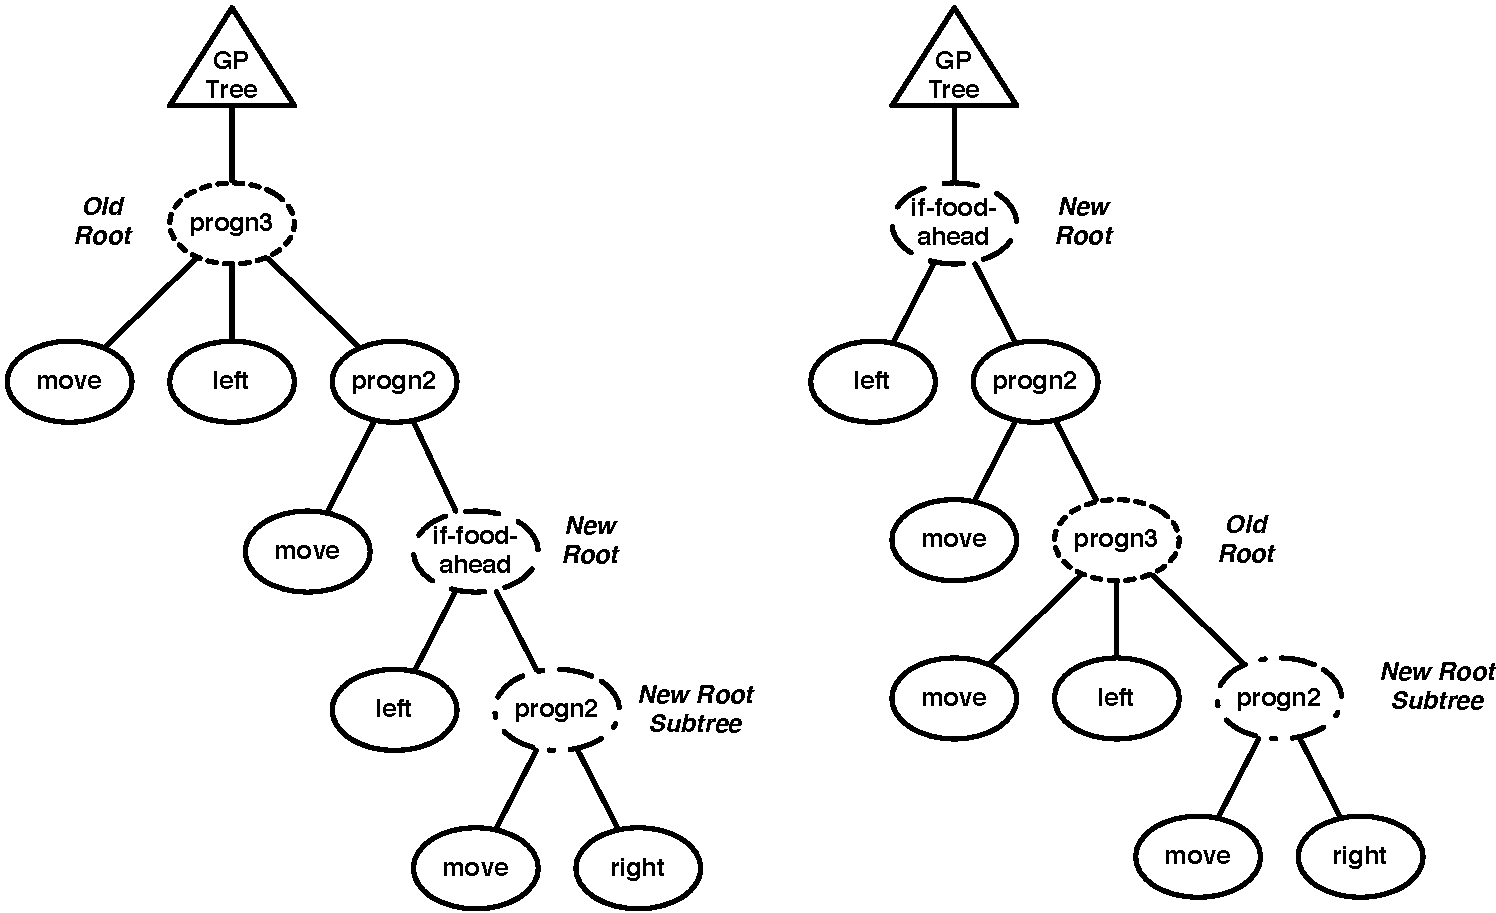
\includegraphics[width=5.5in]{rehang.pdf}
\end{center}
\caption{Rehanging a tree.  A new root is chosen at random from among the nonterminals except for the original root.  Then a subtree of that new root is chosen at random and disconnected.  The tree is then rehung as shown: the parent of the new root becomes its child; the grandparent becomes the parent's child, and so on up to the root.  The disconnected subtree then fills the remaining spot.}
\label{rehang}
\end{figure}
    

\item \class{ec.gp.breed.RehangPipeline} is an oddball mutator of my own design mean to be highly destructive.  It selects a nonterminal other than the root, and designates it the ``new root''.  It then picks a child subtree of this new root, which is disconnected from its parent.  The new root becomes the root of the tree.  The original parent of the new root becomes the new root's child, filling the spot vacated by the disconnected subtree.  The grandparent then fills the spot vacated by the parent, and so on, clear up to the root.  Then finally the disconnected subtree fills remaining spot. Figure \ref{rehang} shows this procedure. There are two parameters, as usual:

\params{%
pop.subpop.0.species.pipe.tries = 1\\
pop.subpop.0.species.pipe.tree.0 = 0
}

The default parameter base versions for all of these would be:

\params{%
gp.breed.rehang.tries = 1\\
gp.breed.rehang.tree.0
}

{\bf Warning: } Because of the complexity of its rehanging process, RehangPipeline ignores all typing information.

\item \class{ec.gp.breed.MutateERCPipeline} works similarly to the {\it Gaussian} algorithm in \cite{chellapilla:1998:piempwsx}.  The algorithm picks a random node in a random tree in the GPIndividual, then for every Ephemeral Random Constant (ERC) in the subtree rooted by that node, it calls \method{mutateERC()} on that ERC.  ERCs are discussed later in Section~\ref{ec.gp.ERC}.  As usual, the two common parameters:s

\params{%
pop.subpop.0.species.pipe.tries = 1\\
pop.subpop.0.species.pipe.tree.0 = 0
}

The default parameter base versions for all of these would be:

\params{%
gp.breed.mutate-erc.tries = 1\\
gp.breed.mutate-erc.tree.0
}

If you wished to mutate the ERCs in the {\it entire tree}, you could set the node selector parameters like this:

\params{%
gp.breed.mutate-erc.ns.0.terminals = 0.0\\
gp.breed.mutate-erc.ns.0.nonterminals = 0.0\\
gp.breed.mutate-erc.ns.0.root = 1.0
}

\end{itemize}



\subsection{A Complete Example}
\label{gpexample}

Much of these initial parameters could have been entered simply by including the parameter file \file{ec/gp/koza/koza.params}.  But we'll go through it in detail.  First some basic generational parameters:
 
\params{%
\# Threads and Seeds\\
evalthreads = 1\\
breedthreads = 1\\
seed.0 = time\\
\\
\# Checkpointing\\
checkpoint = false\\
checkpoint-modulo = 1\\
prefix = ec\\
\\
\# The basic setup\\
state = ec.simple.SimpleEvolutionState\\
finish = ec.simple.SimpleFinisher\\
exch = ec.simple.SimpleExchanger\\
breed = ec.simple.SimpleBreeder\\
eval = ec.simple.SimpleEvaluator\\
stat = ec.simple.SimpleStatistics\\
pop = ec.Population\\
pop.subpops = 1\\
pop.subpops.0 = ec.Subpopulation\\
pop.subpop.0.duplicate-retries = 0\\
pop.subpop.0.size = 1024\\
breed.elite.0 = 0\\
stat.file = \$out.stat\\
quit-on-run-complete = true
}

Genetic programming typically doesn't run very long, and (for the time being) require their own Initializer.  We'll also use KozaFitness.  Following the {\it lil-gp} example, we'll set the duplicate retries to 100:

\params{%
init = ec.gp.GPInitializer\\
generations = 51\\
pop.subpop.0.species.fitness = ec.gp.koza.KozaFitness\\
pop.subpop.0.duplicate-retries = 100
}

For good measure, let's attach KozaShortStatistics to the statistics chain.  This isn't standard in the \file{koza.params} file, but what the heck.

\params{%
stat.num-children = 1\\
stat.child.0 = ec.gp.koza.KozaShortStatistics\\
stat.child.0.gather-full = true\\
stat.child.0.file = \$out2.stat
}

Our initializer will work by using HalfBuilder to build trees.  We define its parameters here:

\params{%
\# HalfBuilder\\
gp.koza.half.min-depth = 2\\
gp.koza.half.max-depth = 6\\
gp.koza.half.growp = 0.5
}

We begin by defining the tree constraints, node constraints, types, and function sets for the problem:

\params{%
\# Types\\
gp.type.a.size = 1\\
gp.type.a.0.name = nil\\
gp.type.s.size = 0\\
\\
\# Basic Function Set Parameters (more later)\\
gp.fs.size = 1\\
gp.fs.0 = ec.gp.GPFunctionSet\\
gp.fs.0.name = f0\\
\\
\# Tree Constraints\\
gp.tc.size = 1\\
gp.tc.0 = ec.gp.GPTreeConstraints\\
gp.tc.0.name = tc0\\
gp.tc.0.fset = f0\\
gp.tc.0.returns = nil\\
gp.tc.0.init = ec.gp.koza.HalfBuilder\\
\\
\# Node Constraints\\
gp.nc.size = 3\\
\\
gp.nc.0 = ec.gp.GPNodeConstraints\\
gp.nc.0.name = nc0\\
gp.nc.0.returns = nil\\
gp.nc.0.size = 0\\
\\
gp.nc.1 = ec.gp.GPNodeConstraints\\
gp.nc.1.name = nc1\\\
gp.nc.1.returns = nil\\
gp.nc.1.size = 1\\
gp.nc.1.child.0 = nil\\
\\
gp.nc.2 = ec.gp.GPNodeConstraints\\
gp.nc.2.name = nc2\\
gp.nc.2.returns = nil\\
gp.nc.2.size = 2\\
gp.nc.2.child.0 = nil\\
gp.nc.2.child.1 = nil
}

Now we define the GP elements of the Species and the Individual:

\params{%
\# Representation\\
pop.subpop.0.species = ec.gp.GPSpecies\\
pop.subpop.0.species.ind = ec.gp.GPIndividual\\
pop.subpop.0.species.ind.numtrees = 1\\
pop.subpop.0.species.ind.tree.0 = ec.gp.GPTree\\
pop.subpop.0.species.ind.tree.0.tc = tc0
}

Here's a basic GP breeding pipeline:

\params{%
\# Pipeline\\
pop.subpop.0.species.pipe = ec.breed.MultiBreedingPipeline\\
pop.subpop.0.species.pipe.generate-max = false\\
pop.subpop.0.species.pipe.num-sources = 2\\
pop.subpop.0.species.pipe.source.0 = ec.gp.koza.CrossoverPipeline\\
pop.subpop.0.species.pipe.source.0.prob = 0.9\\
pop.subpop.0.species.pipe.source.1 = ec.breed.ReproductionPipeline\\
pop.subpop.0.species.pipe.source.1.prob = 0.1
}

For no good reason, we'll define the selection methods, and various other parameters using the default parameter bases for CrossoverPipeline and ReproductionPipeline:

\params{%
\# Reproduction\\ 
breed.reproduce.source.0 = ec.select.TournamentSelection\\
\\
\# Crossover\\
gp.koza.xover.source.0 = ec.select.TournamentSelection\\
gp.koza.xover.source.1 = same\\
gp.koza.xover.ns.0 = ec.gp.koza.KozaNodeSelector\\
gp.koza.xover.ns.1 = same\\
gp.koza.xover.maxdepth = 17\\
gp.koza.xover.tries = 1\\
\\
\# Selection\\
select.tournament.size = 7
}

Since Crossover is using a node selector, let's define some parameters for that:

\params{%
\# Node Selectors\\
gp.koza.ns.terminals = 0.1\\
gp.koza.ns.nonterminals = 0.9\\
gp.koza.ns.root = 0.0
}

Let's presume that we have created the \class{X}, \class{Y}, \class{Sin}, \class{Mul}, and \class{Sub} methods described in Section~\ref{definingtherepresentation}.  We'll now hook them up.

\params{%
\# Our Function Set\\
gp.fs.0 = ec.gp.GPFunctionSet\\
gp.fs.0.size = 5\\
gp.fs.0.func.0 = ec.app.myapp.X\\
gp.fs.0.func.0.nc = nc0\\
gp.fs.0.func.1 = ec.app.myapp.Y\\
gp.fs.0.func.1.nc = nc0\\
gp.fs.0.func.2 = ec.app.myapp.Mul\\
gp.fs.0.func.2.nc = nc2\\
gp.fs.0.func.3 = ec.app.myapp.Sub\\
gp.fs.0.func.3.nc = nc2\\
gp.fs.0.func.4 = ec.app.myapp.Sin\\
gp.fs.0.func.4.nc = nc1
}

Also we're using the \class{MyProblem} and \class{MyData} classes defined in Section~\ref{definingtherepresentation} as our Problem.  Even though we're not using ADFs (see Section~\ref{ec.gp.ADF}), we need to define a few items here as well.

\params{%
\# Our Problem
eval.problem = ec.app.myapp.MyProblem\\
eval.problem.data = ec.app.myapp.MyData\\
gp.problem.stack = ec.gp.ADFStack\\
gp.adf-stack.context = ec.gp.ADFContext
}

Phew!  That was a lot of parameters.  Thankfully nearly all of them are already defined for you in \file{ec/gp/koza/koza.params}.


\subsection{GPNodes in Depth}

GPNode has a gazillion utility methods to assist various crossover, mutation, statistics, and tree-building operators in their tasks of making, breaking, printing, reading, writing and examining trees of GPNodes.  Let's look at some of them here, and divvy up the rest in later sections where they're more appropriate.

First, the two abstract methods which you {\it must} override:

\java{%
public String toString();\\
    public abstract void eval(EvolutionState state,
        int thread,
        GPData input,\\
\hsp{\fill}ADFStack stack,
        GPIndividual individual,
        Problem problem);
}

The first method prints out the node in a human-readable fashion, with no whitspace.  Except for rare cases such as Ephemeral Random Constants (Section~\ref{ec.gp.ERC}), this should be a single simple symbol like ``cos'' or ``if-food-ahead''.  The second method we introduced in Section~\ref{definingtherepresentation}, of course.

One method which is commonly overridden by example applications in ECJ, but it's not necessary for you to do so:

\java{%
public void checkConstraints(EvolutionState state,
        int tree,
        GPIndividual typicalIndividual,
        Parameter individualBase)
}

This method is called after the prototypical GPNode is loaded into a function set to give it an opportunity to  double-check that everything is okay: that the GPNode has the right number of children, that it {\it has} children, that it has a parent, etc., and issue an error if not.   The primary function of this method is to allow Automatically Defined Functions (Section~\ref{ec.gp.ADF}) a chance to make sure that everything is working.  You don't really need to override this method (if you do, be sure to call \method{super(...)}) but you'll see it often implemented in the examples.

Next come some methods which are usually overridden by Ephemeral Random Constants but rarely by any other kind of GPNode (the default implementation suffices):

\begin{methods}{ec.gp.GPNode}
\mthd{public String name()}
Returns the name of the GPNode.  By default, this calls \method{toString().}
\mthd{public int nodeHashCode()}
Returns a hash code appropriate to your GPNode (hash by value, not by address).
\mthd{public boolean nodeEquals(GPNode \textit{node})}
Returns true if this method is identical to the given node.
\mthd{public boolean nodeEquivalentTo(GPNode \textit{node})}
Returns true if the two nodes are the same ``kind'' of node\,---\,usually meaning they could have been cloned from the same prototype node.  The default form of this function returns true if the two nodes are the same class, have the same length child array, and have the same constraints.  Often \method{nodeEquals(...)} and \method{nodeEquivalentTo(...)} may return the same thing, but in Ephemeral Random Constants, they often return different values.  For example, two ERCs that are the same class, and have the same constraints, may hold different values (\variable{2.34} vs. \variable{3.14} say).  These ERCs would be equivalent to one another but not equal to one another.   You'd rarely need to override this method.
\mthd{public String toStringForHumans()}
Writes the node to a String in a fashion readable by humans.  The default version simply calls \method{toString}.
\mthd{public void resetNode(EvolutionState \textit{state}, int \textit{thread})}
Randomizes the node.  Ephemeral Random Constants randomize their internal values; other GPNodes typically do nothing.
\end{methods}

Next, some test functions:

\begin{methods}{ec.gp.GPNode}
\mthd{public int atDepth()}
Returns the depth of the node (the root is at depth 0).
\mthd{public int depth()}
Returns the depth of the subtree rooted by the node (terminals have a subtree depth of 1).
\mthd{public GPNodeParent rootParent()}
Returns the parent of the root of the tree in which the GPNode resides.  Though the method returns a GPNodeParent, this returned object should always be some kind of GPTree.
\mthd{public boolean contains(GPNode \textit{subnode})}
Returns true {\it subnode} exists somewhere within the subtree rooted by the GPNode.
\mthd{public pathLength(int \textit{nodesearch})}
Returns the sum of all paths from all nodes in the GPNode's subtree to the GPNode itself.  The {\it nodesearch} parameter allows us to restrict which nodes have paths included in the sum: only leaf nodes (terminals), non-leaf nodes (nonterminal), or all nodes:

\java{%
    public static final int \textit{GPNode.}NODESEARCH\_ALL;\\
    public static final int \textit{GPNode.}NODESEARCH\_TERMINALS;\\
    public static final int \textit{GPNode.}NODESEARCH\_NONTERMINALS;
}

\mthd{public int numNodes(int \textit{nodesearch})}
Returns the number of nodes in the subtree rooted by GPNode.  The {\it nodesearch} parameter allows us to restrict which nodes are included in the total, using the constants above.
\mthd{public int meanDepth(int \textit{nodesearch})}
Returns the path length divided by the number of nodes.The {\it nodesearch} parameter allows us to restrict which nodes are included in the total, using the constants above.
\end{methods}

Two methods permit even more flexibility in filtering exactly which GPNodes you want to consider, by using a \class{ec.gp.GPNodeGatherer} object.  This object contains a single method which you may override:

\java{%
 public boolean test(GPNode thisNode);
}

In a subclass, override this method to return true if the node provided is one which you'd like to include.  The default form simply returns true for all nodes.  Armed with a GPNodeGatherer you've constructed, you can then call one of the two GPNode methods:

\begin{methods}{ec.gp.GPNode}
\mthd{public int numNodes(GPNodeGatherer \textit{gatherer})}
Returns the number of nodes (filtered by the GPNodeGatherer) in the subtree rooted by the GPNode.
\mthd{public int nodeInPosition(int \textit{p}, GPNodeGatherer \textit{gatherer}, int \textit{nodesearch})}
returns the \(p\)th node in the subtree, filtered either by one of the following node search constants (note there are four here, whereas there were three in the previous methods):

\java{%
    public static final int \textit{GPNode.}NODESEARCH\_ALL;\\
    public static final int \textit{GPNode.}NODESEARCH\_TERMINALS;\\
    public static final int \textit{GPNode.}NODESEARCH\_NONTERMINALS;\\
    public static final int \textit{GPNode.}NODESEARCH\_CUSTOM;
}

In the case of the first three constants, the GPNodeGatherer should be \variable{null}.  The fourth constant indicates that we should use the GPNodeGatherer instead (and it must be provided).
\end{methods}

And now we come to rigamarole which should look familiar to you if you've trudged through the Vector chapter.

\begin{methods}{ec.gp.GPNode}
\mthd{public int printNodeForHumans(EvolutionState \textit{state}, int \textit{log})}
Prints a node to a log in a fashion readable by humans.  You don't want to override this method: it calls \method{toStringForHumans()} by default\,---\,override that instead.
\mthd{public int printNode(EvolutionState \textit{state}, int \textit{log})}
Prints a node to a log in a fashion readable by humans and also parsable by \method{readNode(...)}.  You don't want to override this method: it calls \method{toString()} by default\,---\,override that instead.
\mthd{public int printNode(EvolutionState \textit{state}, PrintWriter \textit{writer})}
Prints a node to a writer in a fashion readable by humans and also parsable by \method{readNode(...)}.  You don't want to override this method: it calls \method{toString()} by default\,---\,override that instead.
\mthd{public String toStringForError()}
Writes a node to a string in a fashion useful for error messages.  The default writes out the name and the tree the node is in, which works fine.
\mthd{public GPNode readNode(DecodeReturn \textit{dret})}
Generates a GPNode from the DecodeReturn via a light clone: children and parents are not produced.  The default version clones the the node, then reads a string from the DecodeReturn.  This string should match \method{toString()} exactly.  If not, returns null to indicate an error.  Otherwise returns the GPNode.  This default implementation should be fine in most cases: though Ephemeral Random Constants (Section~\ref{ec.gp.ERC}) require a different procedure.
 \mthd{public void writeNode(EvolutionState \textit{state}, DataOutput \textit{output}) throws IOException}
Writes the node, but not any of its children or parents, out to {\it output}.
 \mthd{public void readNode(EvolutionState \textit{state}, DataInput \textit{input}) throws IOException}
Reads a node from {\it input}.  Children and parents are not produced.
\end{methods}

Last are a host of different ways of cloning a GPNode or tree.  In most cases the default implementations work just fine:

\begin{methods}{ec.gp.GPNode}
\mthd{public GPNode lightClone()}
Light-clones a GPNode, including its children array, but not any children or parents.
\mthd{public Object clone()}
Deep-clones a GPNode, except for its parent.  All children are cloned as well.
\mthd{public final GPNode cloneReplacing(GPNode \textit{newSubtree}, GPNode \textit{oldSubtree})}
Deep-clones a GPNode, except that, if found within its cloned subtree, {\it oldSubtree} is replaced with a deep-cloned version of \textit{newSubtree}.
\mthd{public final GPNode cloneReplacing(GPNode[] \textit{newSubtrees}, GPNode[] \textit{oldSubtrees})}
Deep-clones a GPNode, except that, if found within its cloned subtree, each of the {\it oldSubtrees} is replaced with a clone of the corresponding member of \textit{newSubtrees}.
\mthd{public final GPNode cloneReplacingNoSubclone(GPNode \textit{newSubtree}, GPNode \textit{oldSubtree})}
Deep-clones a GPNode, except that, if found within its cloned subtree, {\it oldSubtree} is replaced with \textit{newSubtree} (not a clone of \textit{newSubtree}).
\mthd{public final GPNode cloneReplacingAtomic(GPNode \textit{newNode}, GPNode \textit{oldNode})}
Deep-clones a GPNode, except that, if found within its cloned subtree, {\it oldNode} is replaced with \textit{newNode} (not a clone of \textit{newNode}).
\mthd{public final GPNode cloneReplacingAtomic(GPNode[] \textit{newNodes}, GPNode[] \textit{oldNodes})}
Deep-clones a GPNode, except that, if found within its cloned subtree, each of the {\it oldNodes} is replaced with the corresponding member of  \textit{newNodes} (not a clone).
\mthd{public final void replaceWith(GPNode \textit{newNode})}
Replaces the GPnode with {\it newNode} right where it lives in its GPTree.
\end{methods}

These are the primary public methods.  There are plenty of other public methods, but they're largely used internally and you'll rarely need them.

\subsection{GPTrees and GPIndividuals in Depth}

Unlike GPNode, there's nothing in a GPTree that you have to override or modify.   It's pretty rare to subclass GPTree, though it's perfectly reasonable to do so.  But there are a number of methods you should be aware of, many of which are probably very familiar by now.  First, let's cover the three non-familiar ones:


\begin{methods}{ec.gp.GPTree}
\mthd{public int treeNumber()}
Returns the position of the GPTree in its GPIndividual's \variable{trees[]} array.  This is an \(O(n)\) operation\,---\,it works by scanning through the array until it finds the GPTree.  If the tree is not found (which would indicate an error), then \variable{GPTree.NO\_TREENUM} is returned.
\mthd{public final void verify(EvolutionState \textit{state})}
An auxillary debugging method which verifies many features of the structure of the GPTree and all of its GPNodes.  This method isn't called by ECJ but has proven useful in determining errors in GPTree construction by various tree building or breeding algorithms.
\mthd{public void buildTree(EvolutionState \textit{state}, int \textit{thread})}
Builds a tree and attaches it to the GPTree, displacing the original, using the tree-generation algorithm defined for its GPTreeConstraints.  No specific tree size is requested.
\end{methods}

Next come cloning and tests for removing duplicates:

\begin{methods}{ec.gp.GPTree}
\mthd{public boolean treeEquals(GPTree \textit{tree})}
Returns true if the GPNodes which make up the GPTree are structured the same and equal in value to one another.  Override this to provide more equality if necessary.
\mthd{public int treeHashCode()}
Returns a hash code generated for the structure and makeup of the GPNodes in the GPTree.  Override this to add additional hash information.
\mthd{public GPTree lightClone()}
Performs a light clone on the GPTree: the GPNodes are not cloned but are instead the pointer to the root is simply copied.
\mthd{public Object clone()}
Performs a deep clone on the GPTree, including all of its GPNodes but not its parent GPIndividual.
\end{methods}

Last, the standard methods for printing and reading:

\begin{methods}{ec.gp.GPTree}
\mthd{public void printTreeForHumans(EvolutionState \textit{state}, int \textit{log})}
Prints the tree in a human-readable fashion to {\it log}.
\mthd{public void printTree(EvolutionState \textit{state}, int \textit{log})}
Prints to {\it log} the tree in a fashion readable both by humans and also by \method{readTree(..., LineNumberReader)}.  By default this uses the Code package (Section~\ref{ec.util.Code}).
\mthd{public void printTree(EvolutionState \textit{state},
        PrintWriter \textit{writer})}
Prints to {\it writer} the tree in a fashion readable both by humans and also by \method{readTree(..., LineNumberReader)}.  By default this uses the Code package.
\mthd{public void readTree(EvolutionState \textit{state},
        LineNumberReader \textit{reader}) throws IOException}
Reads a tree produced by \method{printTree(...)}.  By default, this uses the Code package (Section~\ref{ec.util.Code}).
\mthd{public void writeTree(EvolutionState \textit{state},
        DataOutput \textit{output}) throws IOException}
Writes a tree to {\it output} in binary fashion such that it can be read by \method{readTree(..., DataInput)}.
\mthd{public void readTree(EvolutionState \textit{state},
        DataInput \textit{input}) throws IOException}
Reads a tree from {\it input} in binary fashion that had been written by \method{writeTree(...)}.
\end{methods}

\subsubsection{Pretty-Printing Trees}

GPTrees have a particular gizmo that's not well known but is quite nice: you can print out GPTrees in one of (at present) four styles:

\begin{itemize}
\item Lisp (the default):  {\small\begin{verbatim}(* (+ x (- (% x x) (cos x))) (exp x))\end{verbatim}}

\item A style easily converted to C, C++, Java, or C\#: {\small\begin{verbatim}(x + ((x % x) - cos(x))) * exp(x)\end{verbatim}}

To print out trees this way you'd use a parameter along these lines (notice the lower-case ``c''):

\params{%
pop.subpop.0.species.ind.tree.0.print-style = c
}

\noindent ...or using the default parameter base:

\params{%
gp.tree.print-style = c
}


Printing in C-style has two options.  First, by default ECJ prints out two-child GPNodes as if they were operators \textstr{b a c} rather than as \textstr{a(b, c)}.  This is what's being done above.  But if you're not using mathematical operators and would prefer to see 2-child GPNodes as functions, you can do it like this:

\params{%
pop.subpop.0.species.ind.tree.0.c-operators = false
}

\noindent ...or using the default parameter base:

\params{%
gp.tree.c-operators = false
}



This results in the following: \begin{verbatim}*(+(x, -(%(x, x), cos(x))), exp(x))\end{verbatim}

This doesn't seem useful for the example here (Symbolic Regression) but for other problems it's probably the right thing to do, particularly if all the GPNodes aren't operators.  Additionally, by default ECJ prints out zero-child GPNodes as constants, as in \textstr{a}, rather than as zero-argument functions, as in \textstr{a()}.  If you'd prefer zero-argument functions, you might say:

\params{%
pop.subpop.0.species.ind.tree.0.c-variables = false
}

\noindent ...or using the default parameter base:

\params{%
gp.tree.c-variables = false
}

This results in the following:\begin{verbatim}x() + ((x() % x()) - cos(x()))) * exp(x())\end{verbatim}

Again, whether this will be useful to you is based on exactly what kind of problem you're emitting.  ECJ does not at present have support for converting if-statements (such as the \textstr{if-food-ahead} node in Artificial Ant) into a brace format appropriate to C.  But hopefully these options will help you get most of the ugly parsing work out the way.


\begin{figure}[t]
\begin{center}
\begin{tabular}{cc}
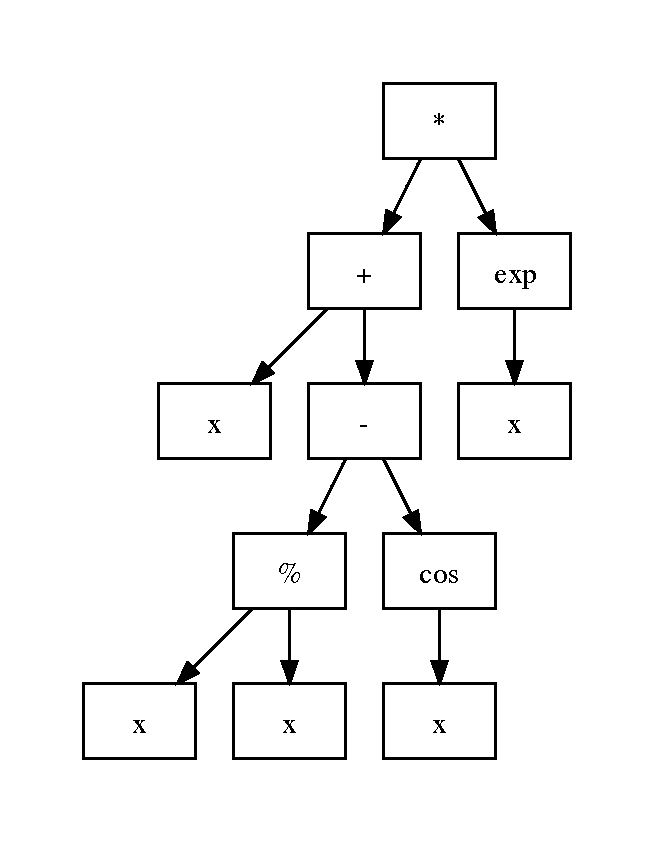
\includegraphics[width=2.4in]{dot.pdf}&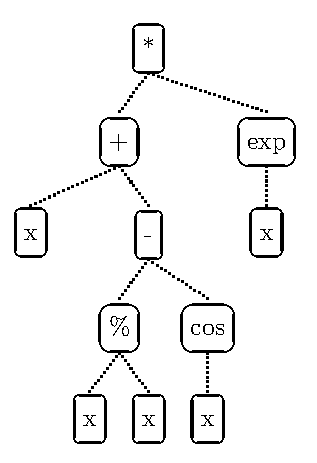
\includegraphics[width=2in]{latextree.pdf}\\
\end{tabular}
\end{center}
\caption{Auto-generated trees: in ``.dot'' format (left) and in \LaTeX{} format (right)}
\label{printedtrees}
\end{figure}

\item \file{.dot} format: used by GraphViz to produce high-quality trees and graphs.  The code below produces the tree shown at left in Figure \ref{printedtrees}:{\small\begin{verbatim}digraph g {
node [shape=rectangle];
n[label = "*"];
n0[label = "+"];
n00[label = "x"];
n0 -> n00;
n01[label = "-"];
n010[label = "%"];
n0100[label = "x"];
n010 -> n0100;
n0101[label = "x"];
n010 -> n0101;
n01 -> n010;
n011[label = "cos"];
n0110[label = "x"];
n011 -> n0110;
n01 -> n011;
n0 -> n01;
n -> n0;
n1[label = "exp"];
n10[label = "x"];
n1 -> n10;
n -> n1;
}\end{verbatim}}

To generate trees in \file{.dot} format, you'd say:

\params{%
pop.subpop.0.species.ind.tree.0.print-style = dot
}

\noindent ...or using the default parameter base:

\params}
\chunk{\gpbox{x}}\chunk{\gpbox{x}}\end{bundle}}\chunk{\begin{bundle}
{\gpbox{cos}}\chunk{\gpbox{x}}\end{bundle}}\end{bundle}}\end{bundle}}
\chunk{\begin{bundle}{\gpbox{exp}}\chunk{\gpbox{x}}\end{bundle}}\end{bundle}
\end{verbatim}}


To generate trees in \LaTeX{} format, you'd say:

\params{%
pop.subpop.0.species.ind.tree.0.print-style = latex
}

\noindent ...or using the default parameter base:

\params'' with ``{\tt \textbackslash\%}'' to make it legal \LaTeX{}.  The code works with the following boilerplate to produce the tree shown at right in Figure \ref{printedtrees}.

{\small\begin{verbatim}
 \documentclass[]{article}
 \usepackage{epic}     % required by ecltree and fancybox packages
 \usepackage{ecltree}  % to draw the GP trees
 \usepackage{fancybox} % required by \Ovalbox

 \begin{document}

 % minimum distance between nodes on the same line
 \setlength{\GapWidth}{1em}    

 % draw with a thick dashed line, very nice looking
 \thicklines \drawwith{\dottedline{2}}   

 % draw an oval and center it with the rule.  You may want to fool with the
 % rule values, though these seem to work quite well for me.  If you make the
 % rule smaller than the text height, then the GP nodes may not line up with
 % each other horizontally quite right, so watch out.
 \newcommand{\gpbox}[1]{\Ovalbox{#1\rule[-.7ex]{0ex}{2.7ex}}}

% And now the code
\begin{bundle}{\gpbox{*}}\chunk{\begin{bundle}{\gpbox{+}}\chunk{\gpbox{x}}
\chunk{\begin{bundle}{\gpbox{-}}\chunk{\begin{bundle}{\gpbox{\%}}
\chunk{\gpbox{x}}\chunk{\gpbox{x}}\end{bundle}}\chunk{\begin{bundle}
{\gpbox{cos}}\chunk{\gpbox{x}}\end{bundle}}\end{bundle}}\end{bundle}}
\chunk{\begin{bundle}{\gpbox{exp}}\chunk{\gpbox{x}}\end{bundle}}\end{bundle}

% Finally end the document
\end{document}
\end{verbatim}
}

\end{itemize}


\subsubsection{GPIndividuals}

Okay, there's not much in-depth here.  GPIndividual implements all the standard Individual methods discussed in Section~\ref{populationsetc}.  Note that the \method{distanceTo(...)} method is {\it not} implemented.  Two methods you might want to be aware of:

\begin{methods}{ec.gp.GPIndividual}
\mthd{public final void verify(EvolutionState \textit{state})}
An auxillary debugging method which verifies many features of the structure of the GPIndividual and ll of its GPTrees (and their GPNodes).  This method isn't called by ECJ but has proven useful in determining errors in GPTree construction by various tree building or breeding algorithms.
\mthd{public long size()}
By default, returns the number of nodes in all the trees held by the GPIndividual.
\end{methods}




\subsection{Ephemeral Random Constants}
\label{ec.gp.ERC}

An {\bf Ephemeral Random Constant} or {\bf ERC} \cite{koza:book} is a special GPNode, usually a terminal, which represents a constant such as \variable{3.14159} or \variable{true} or \variable{724} or \variable{complex: 3.24 \(+\) 5i} or \variable{``aegu''}.  Usually ERCs are used to add constants to programs which rely on math (such as Symbolic Regression).

An ERC needs to be able to do three things:

\begin{itemize}
\item Set itself to a random value when first created.
\item Mutate to a new value when asked to do so.
\item Stay fixed at that value all other times (as a constant).
\end{itemize}

In ECJ, ERCs are usually subclasses of \class{ec.gp.ERC}, an abstract superclass which provides basic functionality.  For example, if we were building a subclass of ERC which represents a floating point numerical constant, we might add a single instance variable to hold its value:

{\small\begin{verbatim}
package ec.app.myapp;
import ec.gp.*;
public class MyERC extends ERC {
    public double value;
    // other methods go here...
    }
\end{verbatim}}

We'll also probably need to implement some or most of the following methods to modify, read, write, or compare the ERC.

\java{%
public String name();\\
public boolean nodeEquals(GPNode node);\\
public int nodeHashCode();\\
public void resetNode(EvolutionState state, int thread);\\
public void mutateERC(EvolutionState state, int thread);\\
public String toStringForHumans();\\
public String encode();\\
public boolean decode(DecodeReturn ret);\\
public void readNode(EvolutionState state, DataInput input) throws IOException\\
public void writeNode(EvolutionState state, DataOutput output)\\
\hsp{\fill}throws IOException\\
public abstract void eval(EvolutionState state,
        int thread,
        GPData input,\\
\hsp{\fill}ADFStack stack,
        GPIndividual individual,
        Problem problem);
}

Let's go through these in turn:

\java{%
public String name();
}

This is not the default GPNode implementation.  When an ERC prints itself out in various ways, it writes its name, then its value.  By default the name is simply ``ERC'', and if you have only one ERC type, you don't have to override it.  For example, an ERC printed out might be \variable{ERC[3.14159]}.  However if you have more than one class of ERCs, holding different kinds of values, you'll want to distinguish them both for humans and for ECJ to read back in again.  To do this, override \method{name()} to return a unique symbol for each kind of ERC.  For example, you might just return ``ERC1'' versus ``ERC2'', resulting in \variable{ERC1[3.14159]} versus \variable{ERC2[921]}.

\java{%
public boolean nodeEquals(GPNode node);\\
public int nodeHashCode();
}

Override the first method to test for equality with the second node: it's the same kind of ERC, the same class, has the same values, etc.  Override the second method to provide a hash code for the ERC based on its type and the values it contains.  By default you can avoid implementing this second method, and just implement the \method{encode()} method, discussed later.  The default version of \method{nodeHashCode()} calls \method{encode()} and then hashes the String.

\java{%
public void resetNode(EvolutionState state, int thread);\\
public void mutateERC(EvolutionState state, int thread);
}

Override the first method to entirely randomize the value of the ERC.  Override the second method to mutate the value of the ERC when called to do so by the MutateERCPipeline.  By default, \method{mutateERC(...)} just calls \method{resetNode(...)}, which is probably not what you want.  Instead the mutation will likely need to be a small deviation from the current value.

\java{%
public String toStringForHumans();\\
public String encode();\\
public boolean decode(DecodeReturn ret);\\
public void readNode(EvolutionState state, DataInput input) throws IOException\\
public void writeNode(EvolutionState state, DataOutput output) throws IOException
}

As usual, override \method{toStringForHumans()} to provide a pretty version of the ERC for human consumption, used by GPNode's printer functions.  The default version just calls \method{toString()}.  You probably want to write something prettier.  The \method{encode()} and \method{decode(...)} methods are supposed to use the Code package (Section~\ref{ec.util.Code}) to encode and decode the ERC in a reasonable fashion. 

Finally, the \method{readNode(...)} and \method{writeNode(...)} methods, as usual, read and write the ERC in binary fashion.  You only need to implement these methods if you're planning on writing over the network (such as using distributed evaluation or island models).  But they're easy so why not?  And of course, there's the method to actually execute the ERC as code.  This typically returns the ERC's internal value (it's a constant after all):

\java{%
    public abstract void eval(EvolutionState state,
        int thread,
        GPData input,\\
\hsp{\fill}ADFStack stack,
        GPIndividual individual,
        Problem problem);
}

\paragraph{Example}

Let's create an ERC and add it to our existing example from Section~\ref{gpexample}.  We'll make an ERC which represents constants between 0.0 and 1.0, not including 1.0.  Our mutator will add a little Gaussian noise to the node.  Here's a full class:

{\small\begin{verbatim}
package ec.app.myapp;
import ec.gp.*;
public class MyERC extends ERC {
    public double value;
    public String toStringForHumans() { return "" + value; }
    public String encode()  { return Code.encode(value); }

    public boolean decode(DecodeReturn ret) {
        int pos = dret.pos;
        String data = dret.data;
        Code.decode(dret);
        if (dret.type != DecodeReturn.T_DOUBLE)  // uh oh!  Restore and signal error.
             { dret.data = data; dret.pos = pos; return false; }
        value = dret.d
        return true;
        }

    public boolean nodeEquals(GPNode node)
        { return (node.getClass() == this.getClass() && ((MyERC)node).value == value); }
        
    public void readNode(EvolutionState state, DataInput input) throws IOException
        { value = dataInput.readDouble(); }
        
    public void writeNode(EvolutionState state, DataOutput output) throws IOException
        { dataOutput.writeDouble(value); }
        
    public void resetNode(EvolutionState state, int thread) 
        { val = state.random[thread].nextDouble(); }
        
    public void mutateNode(EvolutionState state, int thread)  {
        double v; 
        do v = value + state.random[thread].nextGaussian() * 0.01; 
        while( v < 0.0 || v >= 1.0 );
        value = v;
        }
        
    public void eval(EvolutionState state, int thread, GPData input, ADFStack stack,
                                                GPIndividual individual, Problem Problem)
        { ((MyData)data).val = value; }
    }
\end{verbatim}}

Now let's set up the parameters to use it.  We'll change the function set.  Our ERC is a terminal so it takes no arguments: we'll use \variable{nc0} as its constraints.


\params{%
\# Our Function Set\\
gp.fs.0 = ec.gp.GPFunctionSet\\
gp.fs.0.size = 6\\
gp.fs.0.func.0 = ec.app.myapp.X\\
gp.fs.0.func.0.nc = nc0\\
gp.fs.0.func.1 = ec.app.myapp.Y\\
gp.fs.0.func.1.nc = nc0\\
gp.fs.0.func.2 = ec.app.myapp.Mul\\
gp.fs.0.func.2.nc = nc2\\
gp.fs.0.func.3 = ec.app.myapp.Sub\\
gp.fs.0.func.3.nc = nc2\\
gp.fs.0.func.4 = ec.app.myapp.Sin\\
gp.fs.0.func.4.nc = nc1\\
gp.fs.0.func.5 = ec.app.myapp.MyERC\\
gp.fs.0.func.5.nc = nc0
}

... and we're done.




\begin{figure}[t]
\begin{center}
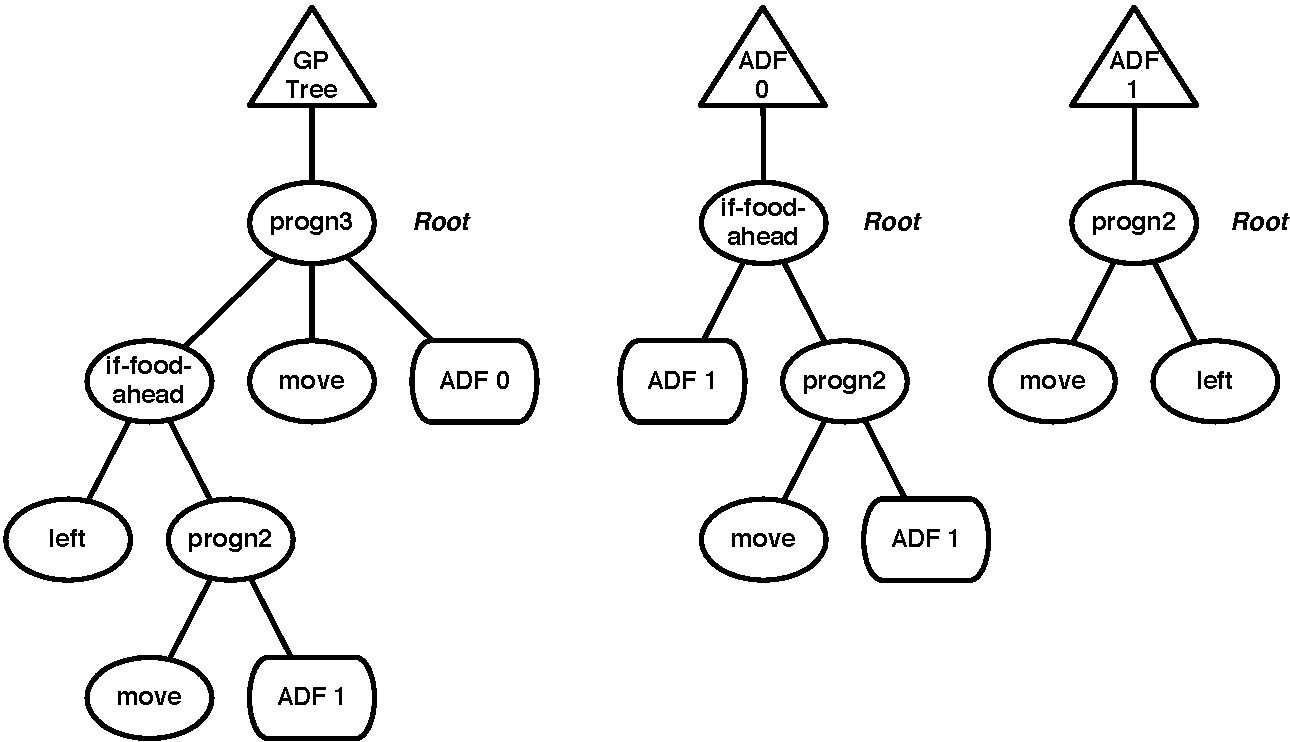
\includegraphics[width=6in]{ADF1.pdf}
\end{center}
\caption{A GPIndividual with two no-argument (terminal) ADFs.  The primary GP Tree has functions in its function set that can call the other two trees; in turn the ADF 1 tree has a function in its function set that can call the ADF 2 tree.  The return values of the various ADF trees become the return values of their respective calling functions.  }
\label{adf1}
\end{figure}

\begin{figure}[t]
\begin{center}
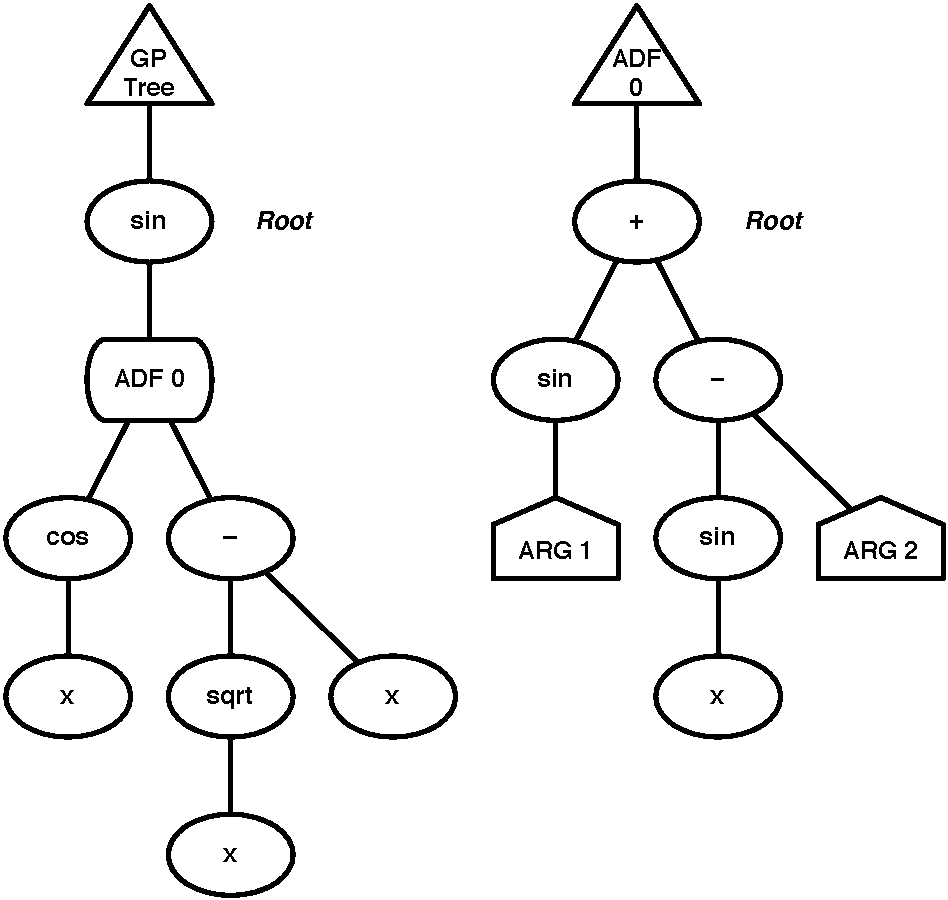
\includegraphics[width=4in]{ADF2.pdf}
\end{center}
\caption{A GPIndividual with one 2-argument ADF.  The primary GP Tree has a function in its function set that can call the ADF tree.  This function first evaluates its children, then executes the ADF tree.   In the ADF tree there are two terminal functions (ARG 1 and ARG 2) which, when evaluated, return the values of the two children respectively.  The return value of the ADF tree becomes the return value of the ADF function.}
\label{adf2}
\end{figure}

\begin{figure}[t]
\begin{center}
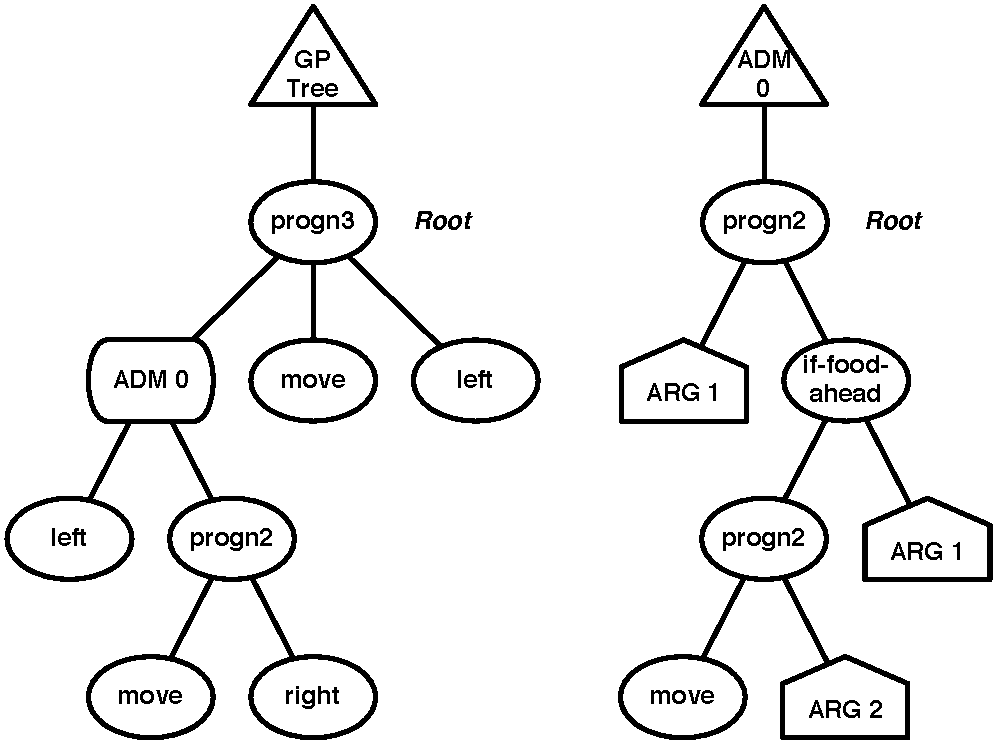
\includegraphics[width=4.25in]{ADM.pdf}
\end{center}
\caption{A GPIndividual with one 2-argument ADM.  The primary GP Tree has a function in its function set that can call the ADM tree.  This function delays the evaluation of its its children, and immediately executes the ADM tree.   In the ADM tree there are two terminal functions (ARG 1 and ARG 2) which, when evaluated, evaluate (or, as necessary, re-evaluate) the original children to the ADM function and then return their values.  Notice that in this example child \# 1 may be evaluated {\it twice}, and child \#2, depending on whether there's food ahead, may be {\it never evaluated}.}
\label{adm}
\end{figure}



\subsection{Automatically Defined Functions and Macros}
\label{ec.gp.ADF}

{\bf Automatically Defined Functions} (ADFs) \cite{koza:gp2} are a standard way of creating some modularism in Genetic Programming.  They define multiple trees in the GPIndividual and essentially define a function calling structure where certain trees can call other trees as subfunctions.  ADFs are the primary reason why GPIndividual has multiple GPTrees.  

The simplest kind of ADF is found in Figure \ref{adf1}.  Here each ADF function is a terminal, and when it is evaluated, it simply evaluates the corresponding ADF tree, then returns the tree's return value.  The ADF function is a GPNode, an instance of \class{ec.gp.ADF}.  It's very rare to further specialize this class.  Notice that calling is nested\,---\,an ADF can call another ADF and so on.  However it's not very common to have {\it recursive} calls because you'll need to construct some kind of stopping base-case criterion to avoid infinite recursive loops.

ADFs add a two more parameters to the standard GPNode suite.  Let's say we're adding a zero-argument ADF.  Beyond the node constraints, we also need to specify which tree will be called when the ADF is executed; and also a simple name for the ADF to distinguish it from other ADFs and GPNodes.  Ideally this name should only have lowercase letters, numbers, and hyphens (that is, ``Lisp-style''):

\params{%
gp.fs.0.func.5 = ec.gp.ADF\\
gp.fs.0.func.5.nc = nc0\\
gp.fs.0.func.5.tree = 1\\
gp.fs.0.func.5.name = ADF0
}

{\bf It's traditional that the first tree be called ADF0, the second ADF1, and so on.}  Since typically the first GP Tree in the array is the ``main'' tree, and the second tree is ADF0, this means that ADF0's associated tree number is usually 1, and ADF1's associated tree number is usually 2.  If you don't specify a name, ECJ will maintain this tradition by setting the name to ``ADF'' \(+\) (tree number \(-\) 1), which is usually right anyway.  It'll also issue a warning.

The name of the ADF (in this case ``ADF1'') and its associated GP tree (in this case, tree 1) are stored in the \class{ec.gp.ADF} class like this:

\java{%
public int associatedTree;\\
public String name;
}

The \method{name()} method returns the value of the \variable{name} variable.

We'll show how to set up the ADF tree itself in the Example below.

ADFs can also have arguments to the functions.  In Figure \ref{adf2}, we have an ADF with two arguments.  The way this works is as follows: when an ADF function is called, we first evaluate its children, then hold their return values in storage.  We then call the corresponding ADF tree.  In that tree there may be one or more special terminal GPNodes, two different kinds of instances of \class{ec.gp.ADFArgument}.  One group of instances, when evaluated, will return the value of the first child.  The second group return the value of the second child.  This enables the ADF tree to use arguments in its ``function call'' so to speak.

ADFArguments add one additional parameter: the child number associated with the argument.  For example:

\params{%
gp.fs.1.func.6 = ec.gp.ADFArgument\\
gp.fs.1.func.6.nc = nc0\\
gp.fs.1.func.5.arg = 0\\
gp.fs.1.func.5.name = ARG0
}

If you don't specify a name, ECJ will set the name to ``ARG'' \(+\) arg number, which is usually right anyway.  It'll also issue a warning.

The ADFArgument's name and argument number are stored in the \class{ec.gp.ADFArgument} class as:

\java{%
public int argument;
public String name;
}

Again, the \method{name()} method returns the value of the \variable{name} variable.

ECJ also supports {\bf Automatically-Defined Macros} (or ADMs), described in \cite{adm}.  These differ from ADFs only in when the children are evaluated.  When an ADM node is evaluated, its children are not evaluated first; rather the ADM immediately calls its associated tree.  When an argument node in that tree (again, a terminal) is evaluated, we teleport back to the associated child and evaluate it right then and there, then return its value.  Note that this means that children may never be evaluated; or can be evaluated multiple times, as shown in Figure \ref{adm}.

ADMs are just like ADFs in their parameters:

\params{%
gp.fs.0.func.6 = ec.gp.ADM\\
gp.fs.0.func.6.nc = nc2\\
gp.fs.0.func.6.tree = 1\\
\# This will be called "ADM1"\\
gp.fs.0.func.6.name = ADM1
}

If an ADF or ADM tree has arguments, it probably will require its own separate GPTreeConstraints, because it needs to have its own GPFunctionSet with those arguments defined.  See the Example below.

\subsubsection{About ADF Stacks}

ADFs and ADMs are a bit complex.  To do their magic, they need a special object called an \class{ec.gp.ADFStack}.  This is actually two stacks of \class{ec.gp.ADFContext} objects which store the location and current return values of various children.  These classes are almost never overridden: here's the standard (default) parameters for them:

\params{%
gp.problem.stack = ec.gp.ADFStack\\
gp.adf-stack.context = ec.gp.ADFContext
}

You {\it could} have defined it this way...

\params{%
eval.problem.stack = ec.gp.ADFStack\\
eval.problem.stack.context = ec.gp.ADFContext
}

... but there are advantages in using the default parameters, particularly when getting to Grammatical Evolution (Section \ref{ec.gp.ge}).

\paragraph{Example}

ADFs and ADMs are fairly straightforward to implement but they can require a fair number of parameters.  Continuing with the example in started in Section~\ref{gpexample} and extended in Section~\ref{ec.gp.ERC}, let's add a 2-argument ADF to the individual.  This will require adding a second GPTree and its own GPTreeConstraints.

Let's begin by modifying the GPFunctionSet of the original tree to include this ADF:

\params{%
\# Our Function Set\\
gp.fs.0 = ec.gp.GPFunctionSet\\
gp.fs.0.size = 7\\
gp.fs.0.func.0 = ec.app.myapp.X\\
gp.fs.0.func.0.nc = nc0\\
gp.fs.0.func.1 = ec.app.myapp.Y\\
gp.fs.0.func.1.nc = nc0\\
gp.fs.0.func.2 = ec.app.myapp.Mul\\
gp.fs.0.func.2.nc = nc2\\
gp.fs.0.func.3 = ec.app.myapp.Sub\\
gp.fs.0.func.3.nc = nc2\\
gp.fs.0.func.4 = ec.app.myapp.Sin\\
gp.fs.0.func.4.nc = nc1\\
gp.fs.0.func.5 = ec.app.myapp.MyERC\\
gp.fs.0.func.5.nc = nc0\\
gp.fs.0.func.6 = ec.gp.ADF\\
gp.fs.0.func.6.nc = nc2\\
gp.fs.0.func.6.tree = 1\\
gp.fs.0.func.6.name = ADF1
}

Let's create a second function set for our second (ADF) tree.  This set will have all the same functions as the main tree, except for the ADF function (we don't want to call ourselves recursively!)  Instead we'll add two ADFArgument nodes to represent the two children.

\params{%
gp.fs.size = 2\\

\# Our Second Function Set\\
gp.fs.1 = ec.gp.GPFunctionSet\\
gp.fs.1.name = f1\\
gp.fs.1.size = 8\\
gp.fs.1.func.0 = ec.app.myapp.X\\
gp.fs.1.func.0.nc = nc0\\
gp.fs.1.func.1 = ec.app.myapp.Y\\
gp.fs.1.func.1.nc = nc0\\
gp.fs.1.func.2 = ec.app.myapp.Mul\\
gp.fs.1.func.2.nc = nc2\\
gp.fs.1.func.3 = ec.app.myapp.Sub\\
gp.fs.1.func.3.nc = nc2\\
gp.fs.1.func.4 = ec.app.myapp.Sin\\
gp.fs.1.func.4.nc = nc1\\
gp.fs.1.func.5 = ec.app.myapp.MyERC\\
gp.fs.1.func.5.nc = nc0\\
gp.fs.1.func.6 = ec.gp.ADFArgument\\
gp.fs.1.func.6.nc = nc0\\
gp.fs.1.func.6.arg = 0\\
gp.fs.1.func.6.name = ARG0\\
gp.fs.1.func.7 = ec.gp.ADFArgument\\
gp.fs.1.func.7.nc = nc0\\
gp.fs.1.func.7.arg = 1
gp.fs.1.func.7.name = ARG1\\
}

Now we create a new GPTreeConstraints which uses this function set:

\params{%
gp.tc.size = 2\\

\# Our Second Tree Constraints\\
gp.tc.1 = ec.gp.GPTreeConstraints\\
gp.tc.1.name = tc1\\
gp.tc.1.fset = f1\\
gp.tc.1.returns = nil\\
gp.tc.1.init = ec.gp.koza.HalfBuilder
}


Next we add the second tree to the GPIndividual:

\params{%
pop.subpop.0.species.ind.numtrees = 2\\
pop.subpop.0.species.ind.tree.1 = ec.gp.GPTree\\
pop.subpop.0.species.ind.tree.1.tc = tc1
}

The ADF stack and ADF context were already defined in the previous examples, but we'll do it again here for clarity:

\params{%
gp.problem.stack = ec.gp.ADFStack\\
gp.adf-stack.context = ec.gp.ADFContext
}

\noindent ...and we're done!

An important note: because the main GP Tree and the ADF have different function sets and thus different GPTreeConstraints, standard GP Crossover (see Section~\ref{gpbreeding}) won't cross over the ADF tree with a main tree of some other individual or vice versa.  But if, for example, your GPIndividual had two ADF trees that had the {\it same} GPTreeConstraints, they could get crossed over with arbitrary other ADF trees in another GPIndividuals.


\subsection{Strongly Typed Genetic Programming}
\label{stronglytyped}

Sometimes it's useful to constrain which GPNodes may serve as children of other GPNodes, or the root of the GPTree.  For example, consider a GPNode called \variable{(if \textit{test} \textit{then} \textit{else})}.  This node evaluates {\it test}, and based on its result (true or false) it either evaluates and returns {\it then} or {\it else}.  Let's presume that {\it then} and {\it else} (and {\it if}) return doubles.  On the other hand, {\it test} is intended to return a boolean.  So you'll need to have some GPNodes in your function set which return doubles and others which return booleans; the \variable{(if ...)} node itself returns a double.

The problem is not that you have nodes which return different values\,---\,this is easily handled by hacking your GPData object.  The problem is that you now have constraints on valid tree structures: you can't plug a node which returns a double (say, \variable{(sin ...)}) into the {\it test} slot of your \variable{(if ...)} node, which is expecting a boolean.\footnote{Well, you {\it could} if you assumed that 0.0 was false and anything else was true.  But this is a hack.  The right way to do it is to constrain things properly}.  This is where strong typing comes in.

ECJ's typing system is simple but sufficient for many common uses.    It's not as sophisticated as a full polymorphic typing system but it also doesn't have the hair-raising complexity that such a system requires.  ECJ is complex enough as it is thank you very much!

ECJ's system is based on {\bf type objects}, subclasses of the abstract superclass \class{ec.gp.GPType}, and nodes are allowed to connect as parent and child if their corresponding type objects are {\bf type compatible}.  ECJ's type objects of two kinds: atomic types and set types.  An atomic type is just a single object (in fact, it's theoretically just a symbol, or in some sense, an integer).  A set type is a set of atomic types. Type compatibility is as follows:

\begin{itemize}
\item Two atomic types are compatible if they are the same.
\item A set type is compatible with an atomic type if it contains the atomic type in its set.
\item Two set types are compatible if their intersection is nonempty.
\end{itemize}

Every GPNode is assigned a type object to represent the ``return type'' of the GPNode.  Furthermore every nonterminal GPNode is assigned a type object for each of its children: this is called the ``child type'' or ``argument type'' or that particular child slot.  Last, the GPTree itself is assigned ``root type'': a type for the root of the tree.  Each GPTree in a GPIndividual can have a different root type.  Here's what must be true about any given GPTree.

\begin{figure}[t]
\begin{center}
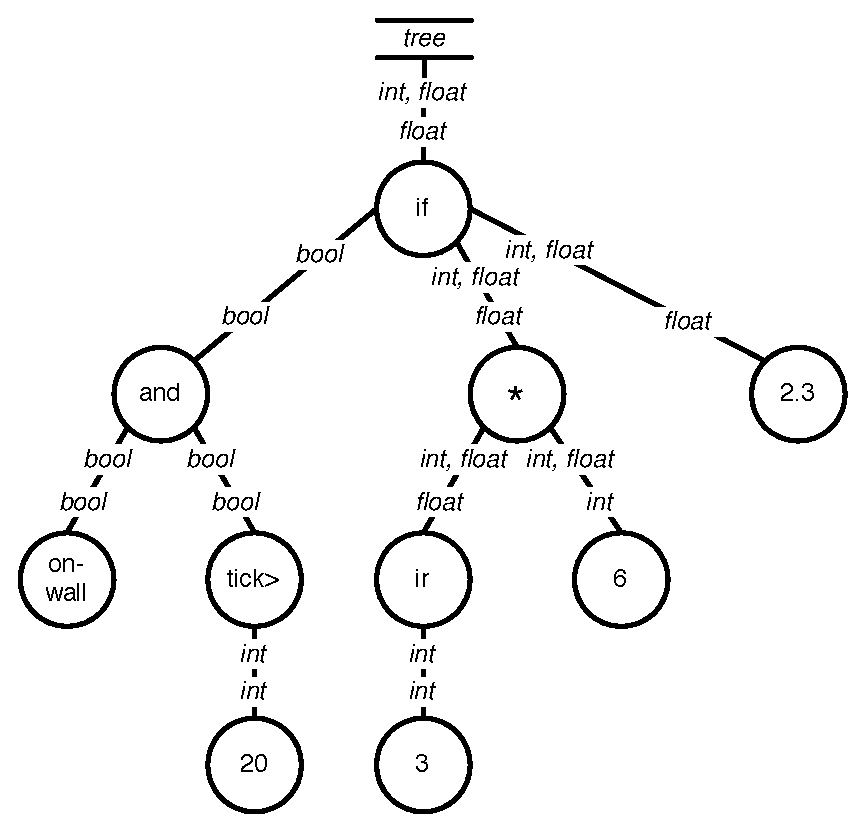
\includegraphics[width=4in]{parsetree.pdf}
\end{center}
\caption{A typed genetic programming parse tree.  Types of the form ``int, float'' are set types.  All others are atomic types.  A repeat of Figure \ref{parsetree}.}
\label{parsetree2}
\end{figure}

\begin{itemize}
\item For any parent and child in a tree, with the child in slot {\it C}, the return type of the child must be compatible with the child type of the parent for slot {\it C}.
\item The return type of the root GPNode must be compatible with the GPTree's root type.  This ensures that the tree is returning 
\end{itemize}

You can see an example of a  GPTree with type constraints listed in Figure \ref{parsetree2}.  

Every GPNodeBuilder and GP Breeding Pipeline must maintain the constraints guaranteed by typing.  The issue is guaranteeing that if you replace one GPNode with another, that the second GPNode will be legal.  This is done primarily with the following two utility functions:

\begin{methods}{ec.gp.GPNode}
\mthd{public GPType parentType(GPInitializer {\it initializer})}
	If the GPNode's parent is another GPNode, this returns the type of the parent's child slot presently filled by the GPNode.  If the GPNode's parent is a GPTree, this returns the type of the tree's root.
\mthd{public final boolean swapCompatibleWith(GPInitializer {\it initializer}, GPNode {\it node})}
	Returns true swapping the GPNode into the slot presently occupied by {\it node} is acceptable, type-wise.
\end{methods}

Before you can assign types, you'll need to define them.  Each type is given a unique symbol.  As an example, let's begin by creating two atomic types, called (uninterestingly) ``boolean'' and ``nil'' (we say ``nil'' instead of ``double'' so we don't have to redefine the GPTreeConstraints and GPNodeConstraints we defined earlier, which all use ``nil'' as their types).  We'd say:

\params{%
gp.type.a.size = 2\\
gp.type.a.0.name = boolean\\
gp.type.a.1.name = nil
}

We might also define a set type or two.  For fun, let's create a set type which contains both booleans and doubles.  We'll also have to stipulate the atomic types encompassed by the set type:

\params{%
gp.type.s.size = 1\\
gp.type.s.0.name = boolean-or-nil\\
gp.type.s.0.size = 2\\
gp.type.s.0.member.0 = boolean\\
gp.type.s.0.member.1 = nil
}

What's the point of set types, you might ask.  Why not just atomic types?  Set types are particularly useful for describing situations where a given GPNode can adapt to several different kinds of children in a given slot.  This is particularly useful for simulating notions of subtyping or subclassing.  For example, a GPNode like \variable{(sin ... )} might declare that its child can either be an ``integer'' or a ``double'', by having its child type defined as a set type of ``number'' which encapsulates both integers and doubles.

What this typing facility {\it cannot} do is dynamically change types as necessary.  For example, you cannot say that a GPNode like \variable{(+ ... ...)} returns a double if either of its children is of type double, but if both of its children are of type integer, then it returns an integer.

You are also restricted to a finite number of types.  For example, consider a GPNode called \variable{(matrix-multiply ... ...)} which takes two children which return matrices.  You cannot say that if the left child is an \(M x N\) matrix, and your right child is an \(N x P\) matrix, that the return type will be an \(M x P\) matrix.  This is partly because you can't define dynamic typing, but it's also because \(M\), \(N\), and \(P\) can be any of an infinite number of numbers, resulting in an infinite number of types: that would be hard on your fingers.  There exist polymorphic typing systems for genetic programming but they're fairly bleeding-edge.  If you need things like this, I suggest instead to look at Grammatical Evolution (Section \ref{ec.gp.ge}).

\paragraph{Example}

Let's add some typing to the example we started in Section~\ref{gpexample} and continued in Sections \ref{ec.gp.ERC} and \ref{ec.gp.ADF}.  We'll add a boolean type as before, and a few functions which rely on it.

First the boolean type:

\params{%
gp.type.a.size = 2\\
gp.type.a.0.name = boolean\\
gp.type.a.1.name = nil
gp.type.s.size = 1\\
gp.type.s.0.name = boolean-or-nil\\
gp.type.s.0.size = 2\\
gp.type.s.0.member.0 = boolean\\
gp.type.s.0.member.1 = nil
}

Next we'll need to modify the node constraints.  We'll not add a new tree constraints because we don't want any trees which return booleans.

For the node constraints, let's add three new GPNodeConstraints:

\begin{itemize}
\item A function which returns a double (nil), has three children, and the first child needs to be a boolean.  The other two children are nil.  This would be for things like the \variable{(if ... ... ...)} node.
\item A function which takes two booleans and returns a boolean.  This would be for functions like \variable{(nand ... ...)}.
\item A function which takes two doubles and returns a boolean.  This would be for functions like \variable{(\(>\) ... ...)}.
\end{itemize}

These three new GPNodeConstraints would be:

\params{%
gp.nc.size = 6\\
\\
\# ... first come the original node constraints, then these:\\
\\
\# Example: (if ... ... ...)\\
gp.nc.3 = ec.gp.GPNodeConstraints\\
gp.nc.3.name = nc3\\
gp.nc.3.returns = nil\\
gp.nc.3.size = 3\\
gp.nc.3.child.0 = boolean\\
gp.nc.3.child.1 = nil\\
gp.nc.3.child.2 = nil\\
\\
\# Example: (nand ...  ...)\\
gp.nc.4 = ec.gp.GPNodeConstraints\\
gp.nc.4.name = nc2\\
gp.nc.4.returns = boolean\\
gp.nc.4.size = 2\\
gp.nc.4.child.0 = boolean\\
gp.nc.4.child.1 = boolean\\
\\
\# Example: (\(>\) ... ...)\\
gp.nc.5 = ec.gp.GPNodeConstraints\\
gp.nc.5.name = nc2\\
gp.nc.5.returns = boolean\\
gp.nc.5.size = 2\\
gp.nc.5.child.0 = nil\\
gp.nc.5.child.1 = nil
}

Recall that our GPData looks like this:

\vbox{\small
\begin{verbatim}
package ec.app.myapp;
import ec.gp.*;
public class MyData extends GPData
    {
    public double val;
    public GPData copyTo(GPData other)
        { ((MyData)other).val = val;  return other;  }
    }
\end{verbatim}
}

We could modify this to include a boolean data type as well, but we'll just use the \variable{val} variable to store both boolean and real-valued data.  Before you go about that, re-read Section \ref{ec.gp.GPData} (on GPData) and its discussion about \method{clone()} and \method{copyTo(...)}.  

Now let's define our three new GPNodes.  First our If-statement:

\vbox{\small\begin{verbatim}
package ec.app.myapp;
import ec.*;
import ec.gp.*;
public class If extends GPNode {
    public String toString() { return "if" };
    public void eval(EvolutionState state, int thread, GPData input,
              ADFStack stack, GPIndividual indivdiual, GPProblem problem) {
        MyData data = (MyData) input;        
        children[0].eval(state, thread, data, stack, individual, prob);
        if (data.val != 0.0) // true
            children[1].eval(state, thread, data, stack, individual, prob);
        else
            children[2].eval(state, thread, data, stack, individual, prob);
        // the result be stored in data
        }
    }
\end{verbatim}
}

Next, the \variable{nand} node:

\vbox{\small\begin{verbatim}
package ec.app.myapp;
import ec.*;
import ec.gp.*;
public class Nand extends GPNode {
    public String toString() { return "nand" };
    public void eval(EvolutionState state, int thread, GPData input,
              ADFStack stack, GPIndividual indivdiual, GPProblem problem) {
        MyData data = (MyData) input;        
        children[0].eval(state, thread, data, stack, individual, prob);
        boolean left = (data.val != 0.0);
        children[1].eval(state, thread, data, stack, individual, prob);
        boolean right = (data.val != 0.0);
        data.val = !(left && right) ? 1.0 : 0.0;
        }
    }
\end{verbatim}
}

Next, the \variable{\(>\)} node:

\vbox{\small\begin{verbatim}
package ec.app.myapp;
import ec.*;
import ec.gp.*;
public class GreaterThan extends GPNode {
    public String toString() { return ">" };
    public void eval(EvolutionState state, int thread, GPData input,
              ADFStack stack, GPIndividual indivdiual, GPProblem problem) {
        MyData data = (MyData) input;        
        children[0].eval(state, thread, data, stack, individual, prob);
        double left = data.val;
        children[1].eval(state, thread, data, stack, individual, prob);
        double right = data.val;
        data.val = (left > right) ? 1.0 : 0.0;
        }
    }
\end{verbatim}
}

Notice that these functions hijack the double value to store boolean information.  This is okay because we {\it know} that the recipient of this information will understand it.  How do we know?  Because the typing constraints have made it impossible to be otherwise.

So let's add these functions to the function set of our main GP Tree:



\params{%
\# Our Main Tree Function Set\\
gp.fs.0 = ec.gp.GPFunctionSet\\
gp.fs.0.size = 10\\
gp.fs.0.func.0 = ec.app.myapp.X\\
gp.fs.0.func.0.nc = nc0\\
gp.fs.0.func.1 = ec.app.myapp.Y\\
gp.fs.0.func.1.nc = nc0\\
gp.fs.0.func.2 = ec.app.myapp.Mul\\
gp.fs.0.func.2.nc = nc2\\
gp.fs.0.func.3 = ec.app.myapp.Sub\\
gp.fs.0.func.3.nc = nc2\\
gp.fs.0.func.4 = ec.app.myapp.Sin\\
gp.fs.0.func.4.nc = nc1\\
gp.fs.0.func.5 = ec.app.myapp.MyERC\\
gp.fs.0.func.5.nc = nc0\\
gp.fs.0.func.6 = ec.gp.ADF\\
gp.fs.0.func.6.nc = nc2\\
gp.fs.0.func.6.tree = 1\\
gp.fs.0.func.6.name = ADF1\\
gp.fs.0.func.7 = ec.app.myapp.If\\
gp.fs.0.func.7.nc = nc3\\
gp.fs.0.func.8 = ec.app.myapp.Nand\\
gp.fs.0.func.8.nc = nc4\\
gp.fs.0.func.9 = ec.app.myapp.GreaterThan\\
gp.fs.0.func.9.nc = nc5\\
}

\noindent ...and we're done!

\paragraph{Mixing ADF and ADMs and Typed GP}  A quick note.  The return type of an ADF node must match the root type of its corresponding ADF tree.  Additionally, the child type of a certain slot in an ADF node must match the return type of the corresponding ADFArgument.  

\subsubsection{Inside GPTypes}  If you want to create a GPNodeBuilder or a GP Breeding Pipeline, you ought to go in more detail about GPTypes.

\class{ec.gp.GPType} is an abstract superclass of \class{ec.gp.GPAtomicType} and \class{ec.gp.GPSetType}, which define the atomic and set types respectively.  The two basic data elements in a GPType are:

\java{%
    public String name;\\
    public int type;
}

The first variable, like GPFunctionSet, GPTreeConstraints, and GPNodeConstraints, holds the name of the type (as defined in the parameters).  The second variable holds a uniquely-assigned integer for this type.  The important feature for types is to determine whether they are {\bf type-compatible} with one another.  The compatibility function is this:

\begin{methods}{ec.gp.GPType}
\mthd{public boolean compatibleWith(GPInitializer {\it initializer}, GPType {\it type})}
Returns true if the return type of this GPNode is type-compatible with the given type.
\end{methods}

GPAtomicTypes are simple: they are compatible with one another if their type integer is the same.  A GPSetType instead is a set of GPAtomicTypes, stored in different ways for query convenience:

\java{%
    public Hashtable types\_h;\\
    public int[] types\_packed;\\
    public boolean[] types\_sparse;
}

The first is the GPAtomicTypes in the set stored in a Hashtable.  The second is an array of the GPAtomicTypes.  And the third is an array of booleans, one for each GPAtomicType number, which is true if that GPAtomicType is a member of the set.

A GPSetType is compatible with a GPAtomicType if the GPSetType contains the GPAtomicType as an element.  Two GPSetTypes are compatible with one another if their intersection is nonempty.



\subsection{Parsimony Pressure (The \package{ec.parsimony} Package)}
\label{ec.parsimony}

Genetic programming has a serious bloat problem: as evolution progresses, the size of the trees inside the population tend to grow without bound.  This is a problem that exists for various arbitrary-length representations (lists, graphs, rulsests, etc.) but genetic programming has studied it the most.

The most common simple way of keeping trees down is to make it illegal to produce a tree larger than a certain depth.  For example, Koza's standard rules, adhered to by the basic parameters in ECJ, stipulate that crossover and mutation operators may not produce a child which is deeper than 17 nodes \cite{koza:book}, for example:

\params{%
gp.koza.xover.tries = 1\\
gp.koza.xover.maxdepth = 17
}

Here if the crossover operation produces a child greater than 17, it is not forwarded on; but rather its (presumably smaller) parent is forwarded on in its stead.  This is a fairly crude approach to parsimony pressure, but it's fairly effective.  Another approach\,---\,which can be done at the same time\,---\,is to modify the selection operator to favor smaller individuals.  This notion is called {\bf parsimony pressure}.

In the \package{ec.parsimony} package, ECJ has several SelectionMethods which select both based on fitness and on size (smaller size being preferred).  These methods compute size based on GPNode's \method{size()} function.  Many of these selection methods were compared and discussed at length in \cite{Luke:2006:EC}.  Here they are:

\begin{itemize}
\item \class{ec,parsimony.LexicographicTournamentSelection} is a straightforward TournamentSelection operator, except that the fitter Individual is preferred (as usual), but when both Individuals are the same fitness, the smaller Individual is preferred. Parameters for this operator are basically the same as for TournamentSelection.

Let us presume that the SelectionMethod is the first source of the pipeline of Subpopulation 0.  Then the basic parameters are the same as in TournamentSelection:

\params{%
pop.subpop.0.species.pipe.source.0 = ec.parsimony.LexicographicTournamentSelection\\
pop.subpop.0.species.pipe.source.0.size = 7\\
pop.subpop.0.species.pipe.source.0.pick-worst = false
}

Or using the default parameters:

\params{%
pop.subpop.0.species.pipe.source.0 = ec.parsimony.LexicographicTournamentSelection\\
select.lexicographic-tournament.size = 7\\
select.lexicographic-tournament.pick-worst = false
}

The problem with this method is that bloat control only comes into effect for problems where lots of fitness ties occur.  This problem lead us to two modifications of the basic idea:

\item \class{ec,parsimony.BucketTournamentSelection} is like LexicographicTournamentSelection, except that first individuals are placed into \(N\) classes (``buckets'') based on fitness. The subpopulation is first sorted by fitness.  Then the bottom \(\frac{\text{subpopulation size}}{N}\) individuals are placed in the worst bucket, plus any individuals remaining in the subpopulation with the same fitness as the best individual in that bucket.  Next the bottom remaining \(\frac{\text{subpopulation size}}{N}\) are placed in the second worst bucket, plus any individuals remaining in the population with the same fitness as the best individual in that bucket.  This continues until all the individuals are exhausted.  BucketTournamentSelection then works like LexicographicTournamentSelection except that instead of comparing based on fitness, it compares based on the bucket the individual is in.  The number of buckets is defined by \parameter{num-buckets}:

\params{%
pop.subpop.0.species.pipe.source.0 = ec.parsimony.BucketTournamentSelection\\
pop.subpop.0.species.pipe.source.0.size = 7\\
pop.subpop.0.species.pipe.source.0.pick-worst = false\\
pop.subpop.0.species.pipe.source.0.num-buckets = 10
}

Or using the default parameters:

\params{%
pop.subpop.0.species.pipe.source.0 = ec.parsimony.BucketTournamentSelection\\
select.bucket-tournament.size = 7\\
select.bucket-tournament.pick-worst = false\\
select.bucket-tournament.num-buckets = 10
}


\item \class{ec,parsimony.ProportionalTournamentSelection} is like TournamentSelection, except that it {\it either} selects based on fitness {\it or} selects based on size.  It determines which one to do by flipping a coin of a certain probability that {\it fitness} will be used.  The parameters are:

\params{%
pop.subpop.0.species.pipe.source.0 = ec.parsimony.ProportionalTournamentSelection\\
pop.subpop.0.species.pipe.source.0.size = 7\\
pop.subpop.0.species.pipe.source.0.pick-worst = false\\
pop.subpop.0.species.pipe.source.0.fitness-prob = 0.9
}

Or using the default parameters:

\params{%
pop.subpop.0.species.pipe.source.0 = ec.parsimony.ProportionalTournamentSelection\\
select.bucket-tournament.size = 7\\
select.bucket-tournament.pick-worst = false\\
select.bucket-tournament.fitness-prob = 0.9
}

\item \class{ec,parsimony.DoubleTournamentSelection} is actually two TournamentSelections in a row.  In short, we do a TournamentSelection of tournament size \(N\) based on fitness: but the entrants to that tournament are not chosen uniformly at random from the subpopulation, but rather are the winners of \(N\) {\it other} tournament selections, each performed based on size.  Alternatively, we can first do tournament selections on fitness, then have a final tournament on size.

Thus there are roughly twice as many parameters: ones describing the final tournament, and ones describing the initial (``qualifying'') tournaments

\params{%
pop.subpop.0.species.pipe.source.0 = ec.parsimony.DoubleTournamentSelection\\
\\
\# Final tournament\\
pop.subpop.0.species.pipe.source.0.size = 2\\
pop.subpop.0.species.pipe.source.0.pick-worst = false\\
\\
\# Qualifying tournaments\\
pop.subpop.0.species.pipe.source.0.size2 = 2\\
pop.subpop.0.species.pipe.source.0.pick-worst2 = false\\
\\
\# Make the qualifying tournament based on size\\
pop.subpop.0.species.pipe.source.0.do-length-first = true
}

Or using the default parameters:

\params{%
pop.subpop.0.species.pipe.source.0 = ec.parsimony.DoubleTournamentSelection\\
\\
\# Final tournament\\
select.double-tournament.size = 7\\
select.double-tournament.pick-worst = false\\
\\
\# Qualifying tournaments\\
select.double-tournament.size2 = 7\\
select.double-tournament.pick-worst2 = false\\
\\
\# Make the qualifying tournament based on size\\
select.double-tournament.do-length-first = true
}


\item \class{ec,parsimony.TarpeianStatistics} implements the ``Tarpiean'' parsimony pressure method \cite{poli03simple}.  This method identifies the individuals in the subpopulation with above-average size.  Notice that this may not be half the subpopulation: it could be a very small number if they are very large and the others are very small.  Then a certain proportion of these individuals, picked randomly, are assigned a very bad fitness, and their \variable{evaluated} flags are set.  This happens {\it before} evaluation, so the evaluation procedure doesn't bother to evaluate those individuals further.

The Tarpiean method isn't a selection procedure: it's a fitness assignment procedure.  As such it's not implemented as a SelectionMethod but rather as a Statistics subclass which hooks into the evolutionary loop prior to evaluation.

Let's say that TarpieanStatistics is the only child of our primary Statistics object.  The parameters would look like this:

\params{%
stat.num-children = 1\\
stat.child.0 = ec.parsimony.TarpeianStatistics\\
stat.child.0.kill-proportion = 0.2
}


\end{itemize} 


\section{Grammatical Evolution (The \package{ec.gp.ge} Package)}
\label{ec.gp.ge}


Grammatical Evolution (GE) \cite{grammaticalevolution}  is an approach to building genetic programming trees using a grammar interpreted by a list representation.  The trees are then evaluated and tested.  In ECJ the procedure for evaluating Individuals in GE works roughly like this.

\begin{itemize}
\item The representation is an arbitrarily long list of bytes (See Section \ref{list}), implemented as a special subclass of ByteVectorIndividual called \class{ec.gp.ge.GEIndividual}.
\item The Fitness is typically a KozaFitness.
\item The GEIndividual's species is a \class{ec.gp.ge.GESpecies}.
\item The GESpecies holds a {\bf grammar}, loaded from a file and produced via an \class{ec.gp.ge.GrammarParser}, which we will interpret according to the bytes in the Individual.
\item To assess the fitness of a GEIndividual, we hand it to the GESpecies which interprets it according to the grammar, producing a GPIndividual.
\item The GPIndividual is then evaluated in the normal ECJ fashion and its Fitness is set.
\item We then transfer the Fitness to the GEIndividual. 
\end{itemize}

We'd like to use plain-old GP test problems to make this as easy as possible.  To pull this off we have to do a few minor hacks.  First, we must insert the GE conversion process in-between the Evaluator and the GPProblem that the user wrote.  To do this we have a special Problem class called \class{ec.gp.ge.GEProblem}, which is assigned as the Evaluator's problem.  The GPProblem is then set up as a subsidiary of the GEProblem.  When the Evaluator wishes to evaluate a ByteVectorIndividual, it calls the GEProblem, which converts it to a GPIndividual and then hands the GPIndividual to the GPProblem to evaluate.  This is done as follows:

\params{%
eval.problem = ec.gp.ge.GEProblem\\
eval.problem.problem = ec.app.myproblem.MyGProblem
}

Note that GPProblems usually require auxiliary parameters (not the least of which is their GPData), so we'll need to also say things like...

\params{%
eval.problem.problem.data = ec.app.myproblem.MyGPData
}

... etc.  You don't need to define the ADFStack or ADFContext specially because the default parameters for them suffice:

\params{%
gp.problem.stack = ec.gp.ADFStack\\
gp.adf-stack.context = ec.gp.ADFContext
}


\subsection{GEIndividuals, GESpecies, and Grammars}
The reason we use GEIndividual instead of just ByteVectorIndividual is simple: when we print out the GEIndividual we wish to print out the equivalent GPIndividual as well.  That's the {\it only} thing GEIndividual does beyond being just a ByteVectorIndividual.  

The GEProblem doesn't actually do the translation from list to tree.  Instead, it calls on the GESpecies to do this dirty work.  First, let's set the GESpecies, GEIndividual, GrammarParser, and Fitness of Species 0:

\params{%
pop.subpop.0.species = ec.gp.ge.GESpecies\\
pop.subpop.0.species.parser = ec.gp.ge.GrammarParser\\
pop.subpop.0.species.ind = ec.gp.ge.GEIndividual\\
pop.subpop.0.species.fitness = ec.gp.koza.KozaFitness
}

GESpecies requires a {\bf grammar file} for each tree in the GPIndividual.  If your GPIndividual has two trees (say), you'll need two grammar files, which are specified like this: 

\params{%
pop.subpop.0.species.file.0 = foo.grammar\\
pop.subpop.0.species.file.1 = bar.grammar
}

Alternatively you can use the default parameter base:

\params{%
ge.species.file.0 = foo.grammar\\
ge.species.file.1 = bar.grammar
}

Grammar files are text files consisting of lines.  Each line can be blank whitespace (which is ignored), a comment (which starts with a \#, just like parameter files), or a {\bf grammar rule}.  A grammar rule has a {\bf head}, followed by whitespace, followed by the string \textstr{::=}, then more whitespace, and finally  a {\bf body}.  Here is an example rule:

\vbox{\small\begin{verbatim}
<foo> ::= (hello <bar>) | (yo) | (whoa <bar> <baz>)
\end{verbatim}}

In this example, \variable{\(<\)foo\(>\)} is the head, and \variable{(hello \(<\)bar\(>\)) \(|\) (yo) \(|\) (whoa \(<\)bar\(>\) \(<\)baz\(>\))} is the body.  The head is always a simple, usually lower-case, symbol surrounded in angle brackets.  The body is a collection of {\bf clauses} separated by the pipe symbol (\ \(|\)\ ).  Each clause is a single GP node in Lisp s-expression form.  For example, \variable{(hello \(<\)bar\(>\))} defines a GP node named \variable{hello}, which has a single child defined by the symbol \variable{\(<\)bar\(>\)}.

Terminal (leaf-node) GPNodes are defined as S-expressions with no children.  For example, \variable{(yo)} is a terminal GPNode whose name is \variable{yo}.  And a GPNode can have more than one child, such as \mbox{\variable{(whoa \(<\)bar\(>\) \(<\)baz\(>\))}}.

For each symbol that appears in the body of a rule in angle brackets, there must be at least one such symbol in a head of a rule.  However you can have multiple such heads:

\vbox{\small\begin{verbatim}
<foo> ::= (hello <bar>)
<foo> ::= (yo) | (whoa <bar> <baz>)
\end{verbatim}}

This says the exact same thing as the previous rule example.  You are free to use pipe symbols or create separate rules with the same head, or mix and match the two.  You can also have plain angle-bracket symbols in the body like this:

\vbox{\small\begin{verbatim}
<foo> ::= (blah <bar>) | <okay>
\end{verbatim}}

This says that \variable{\(<\)foo\(>\)} can expand to either the GPNode \variable{blah} or it can expand to whatever \variable{\(<\)okay\(>\)} expands to.  You'd probably want to watch out for recursive definitions.  For example, these wouldn't be great rules:

\vbox{\small\begin{verbatim}
<foo> ::= (blah <bar>) | <okay>
<okay> ::= <foo> | (yuck)
\end{verbatim}}

The {\bf head of the first rule in the file} is the entry point of the grammar and represents the root node of the GPTree.  In all of our examples we have called it \variable{\(<\)start\(>\)}, but it doesn't have to be that.  For example, here is a complete grammar for a very simple tree which produces the same kinds of GPIndividuals as described in the example in Section \ref{definingtherepresentation}:

\vbox{\small\begin{verbatim}
<start> ::= <op>
<op> ::= (x) | (y)
<op> ::= (sin <op>) | (* <op> <op>) | (- <op> <op>)
\end{verbatim}}

\subsubsection{Strong Typing}

At this point we don't see a lot of power.  But Grammatical Evolution can define all sorts of typing requirements by specifying which symbols appear where in rules.  For example, we could extend this grammar to handle the Strongly-Typed Genetic Programming example shown in Section \ref{stronglytyped}:

\vbox{\small\begin{verbatim}
<start> ::= <op>
<op> ::= (x) | (y) | (sin <op>) | (* <op> <op>) | (- <op> <op>)
<op> ::= (if <bool> <op> <op>)
<bool> ::= (nand <bool> <bool>)
<bool> ::= (> <op> <op>)
\end{verbatim}}

If you have a grammar like this, you'd imagine it would need to be accompanied by GPNodes that have been appropriately typed in a strongly typed context.  But it's not true.  Recall that strong typing is intended to provide constraints for building trees, mutating them, and crossing them over using traditional GP methods.  But since Grammatical Evolution is doing all of this based on a list of bytes, GPTypes serve no function.

As a result, you should just have a single GPType even in a ``strongly typed'' example such as the one above.  You can have more if you like, but it serves no purpose and may trip you up.

\subsubsection{ADFs and ERCs}
Each GPNode in the grammar is looked up according to its name.  Thus if you have a grammar element called \((sin ...)\), you'll need to have a GPNode whose \method{name()} method returns \variable{sin}.  This goes for ERCs and ADFs as well.  Typically the \method{name()} of an ERC is simply \variable{ERC}, the \method{name()} of an ADF is something like \variable{ADF1}, and the \method{name()} of an ADFArgument is often something like \variable{ARG0}.  Thus you might have a grammar that looks like:

\vbox{\small\begin{verbatim}
<start> ::= <op>
<op> ::= (x) | (y) | (sin <op>) | (* <op> <op>) | (- <op> <op>)
<op> ::= (ERC)
<op> ::= (ADF1 <op> <op>)
\end{verbatim}}

\subsection{Translation and Evaluation}

Translation is done as follows.  GESpecies is handed a GEIndividual, which is little more than an arbitrary-length ByteVectorIndividual.  You should set this GEIndividual to have maximal min-gene and max-gene values, so it can have any of all 256 possible settings per gene:

\params{%
pop.subpop.0.species.min-gene = -128\\
pop.subpop.0.species.max-gene = 127
}

GESpecies starts working through the byte array and the grammar, depth-first. Each time GESpecies comes across a point in the  grammar where multiple expansions are possible, it consults the next byte in the byte array.  Let's say there are four possible expansions of the head \variable{\(<\)foo\(>\)}, and the next byte says 145.  We compute \(145 \mod 4 = 1\) and so pick expansion 1 (the second expansion --- the first one is expansion 0).

This continues until one of two things happens.  Either the tree is completed, or we run out of bytes.  In the first case, the tree is finished and the GEProblem hands it to the GPProblem to be evaluated.  In the second case,  the fitness is simply set to the worst possible Koza Standardized Fitness (\variable{Float.MAX\_VALUE}).

If the GEIndividual is valid and the GPIndividual is then set to the GPProblem to be evaluated, after evaluation, the GEIndividual's fitness is set to the GPIndividual's fitness, the GEIndividal's \variable{evaluated} flag is set to the GPIndividual's flag, and evaluation of the GEIndividual is completed.

To do the translation, GESpecies relies on certain methods that may be useful to you:

\begin{methods}{ec.gp.ge.GESpecies}
\mthd{public int makeTree(EvolutionState \textit{state}, GEIndividual \textit{ind}, GPTree \textit{tree}, int \textit{position}, int \textit{treeNum},}
\hsp{\fill}{\sf int \textit{threadnum})}\\
Builds a GPTree from a GEIndividual.  The tree is stored in {\it tree}.  The tree number (and thus the particular grammar to be used) is defined by {\it treeNum}.  Bytes are read from the GEIndivdidual starting at \textit{position}.  When the tree has been generated, the first unread byte position is returned.  If the tree could not be built because there were not enough bytes, then \variable{ec.gp.ge.GESpecies.BIG\_TREE\_ERROR} is returned instead.
\mthd{public int makeTrees(EvolutionState \textit{state}, GEIndividual \textit{ind}, GPTree[] \textit{trees}, int \textit{threadnum})}
Builds an entire array of GPTrees, sufficient to create an entire GPIndividual, from a GEIndividual.  The trees are stored in {\it trees}.  Bytes are read from the GEIndivdidual starting at position 0.  When the tree has been generated, the first unread byte position is returned.  If the trees could not be built because there were not enough bytes, then \variable{ec.gp.ge.GESpecies.BIG\_TREE\_ERROR} is returned instead.
\mthd{public int consumed(EvolutionState \textit{state}, GEIndividual \textit{ind}, int \textit{threadnum})}
Computes and returns the number of bytes that would be consumed to produce a GPIndividual from the given GEIndividual. This is done by actually building an individual, then throwing it away.  If the GPIndividual could not be built because there were not enough bytes, then \variable{ec.gp.ge.GESpecies.BIG\_TREE\_ERROR} is returned instead.
\end{methods}

\paragraph{Handling ERCs}  When the GESpecies needs to produce an ERC from the grammar, it consults the next byte in the array.  If the byte is 192, it looks up 192 in a special hash table stored in GESpecies.  If it finds that 192 has hashed to an existing ERC, it clones this ERC and uses the clone.  Else, it creates a new ERC, calls \method{reset()} on it, stores it in the hash table with 192, clones it, and uses the clone.  This way all ERCs whose byte is 192 are the same value.

\paragraph{Handling ADFs and Multiple Trees}  Recall that the GESpecies maintains a separate grammar for each tree in the GPIndividual (and thus for each separate ADF).  However there's only a single byte array in the GEIndividual.  This is handled straightforwardly the array is used to build the first tree; then the unused remainder of the array is used to build the second tree; and so on.  If not all trees were able to be built, evaluation of the GPIndividual is bypassed and the fitness is set to the (\variable{Float.MAX\_VALUE}).

\paragraph{Grammatical Evolution Does Not Support GroupedProblemForm}  GroupedProblemForm evaluates several Individuals together.  What if at least one of them is a GEIndividual, and the GEIndividual cannot generate a valid GPIndividual?  This creates a number of hassles.  For example, if we're doing cooperative coevolution, and one Individual can't be generated, what's the fitness of the group?  Is it fair to penalize the group thusly?  Likewise if we're doing competitive coevolution, and one of the competitors can't be generated, what's the resulting fitness of the other?  For this reason, at present Grammatical Evolution does not support GroupedProblemForm.

\subsection{Initialization and Breeding}

Since we're doing lists, we'll need to define the parameters for creating new lists in the first place.  The default parameters in \file{ge.params} do geometric size distribution as follows:

\params{%
pop.subpop.0.species.genome-size = geometric\\
pop.subpop.0.species.geometric-prob = 0.85\\
pop.subpop.0.species.min-initial-size = 5
}

Change this to your heart's content.

While we could use things like ListCrossoverPipeline, GE has two idiosyncratic list breeding operators:

\begin{itemize}

\item \class{ec.vector.breed.GeneDuplicationPipeline} picks two random indices in the list, copies the byte sequence between them, then tacks the copy to the end of the list.  Because this doesn't rely on anything special to GE, it's located in \package{ec.breed.vector}.

\item \class{ec.gp.ge.breed.GETruncationPipeline} determines how many bytes were consumed in the production of the GPTree.  It then truncates the list to remove the unused bytes.

\end{itemize}

The default pipeline in \file{ge.params} is a MultiBreedingPipeline which with 0.9 probability performs GETruncation, followed by crossover; and with 0.05 probability performs GETruncation followed by GeneDuplication; and 0.05 probability simply does plain VectorMutation.  In all cases we use Tournament Selection with size of 7.

\params{%
pop.subpop.0.species.pipe = ec.breed.MultiBreedingPipeline\\
pop.subpop.0.species.pipe.num-sources = 3\\
\\
pop.subpop.0.species.pipe.source.0 = ec.vector.breed.ListCrossoverPipeline\\
pop.subpop.0.species.pipe.source.0.source.0 = ec.gp.ge.breed.GETruncationPipeline\\
pop.subpop.0.species.pipe.source.0.source.0.source.0~=~ec.select.TournamentSelection\\
pop.subpop.0.species.pipe.source.0.source.1 = same\\
pop.subpop.0.species.pipe.source.0.prob = 0.9\\
\\
pop.subpop.0.species.pipe.source.1 = ec.vector.breed.GeneDuplicationPipeline\\
pop.subpop.0.species.pipe.source.1.source.0 = ec.gp.ge.breed.GETruncationPipeline\\
pop.subpop.0.species.pipe.source.1.source.0.source.0~=~ec.select.TournamentSelection\\
pop.subpop.0.species.pipe.source.1.prob = 0.05\\
\\
pop.subpop.0.species.pipe.source.2 = ec.vector.breed.VectorMutationPipeline\\
pop.subpop.0.species.pipe.source.2.source.0 = ec.select.TournamentSelection\\
pop.subpop.0.species.pipe.source.2.prob = 0.05\\
\\
select.tournament.size = 7
}

You are of course welcome to change this any way you like.

The default pipeline also defines the mutation probability for VectorMutationPipeline, and includes a crossover type even though it's unused (to quiet complaints from ECJ):

\params{%
pop.subpop.0.species.mutation-prob = 0.01\\
\# This isn't used at all but we include it here to quiet a warning from ECJ\\
pop.subpop.0.species.crossover-type = one
}

\subsection{Dealing with GP}

Once you've created your grammar and set up your GEIndividual and GESpecies, you'll still need to define all the same GPNodes, GPFunctionSets, GPNodeConstraints, GPTreeConstraints, etc. as usual.  All GE is doing is giving you a new way to breed and create trees: but the tree information must still remain intact.  However, certain items must be redefined because the GPSpecies is no longer in the normal parameter base (\parameter{pop.subpop.0.species}) but rather is the subsidiary to GESpecies, and thus at the parameter base (\parameter{pop.subpop.0.species.gp-species}).  The simplest way to do this is to include \file{ec/gp/koza/koza.params} to define all the basic GP stuff, then create all of your GPNodes etc., and then override certain GP parameters, namely:

\params{%
\# We define a dummy KozaFitness here, and set the number of trees to 1.\\
\# If you're doing ADFs, you'll need to add some more trees.\\
pop.subpop.0.species.gp-species = ec.gp.GPSpecies\\
pop.subpop.0.species.gp-species.fitness = ec.gp.koza.KozaFitness\\
pop.subpop.0.species.gp-species.ind = ec.gp.GPIndividual\\
pop.subpop.0.species.gp-species.ind.numtrees = 1\\
pop.subpop.0.species.gp-species.ind.tree.0 = ec.gp.GPTree\\
pop.subpop.0.species.gp-species.ind.tree.0.tc = tc0\\

\# We also need a simple dummy breeding pipeline for GP, which will never\\
\# be used, but if it's not here GP will complain.  We'll just use Reproduction.\\
pop.subpop.0.species.gp-species.pipe = ec.breed.ReproductionPipeline\\
pop.subpop.0.species.gp-species.pipe.num-sources = 1\\
pop.subpop.0.species.gp-species.pipe.source.0 = ec.select.TournamentSelection\\
}

This is enough to convince the GP system to go along with our bizarre plans.

\subsection{A Complete Example}

We will continue the example given in Section \ref{stronglytyped}.  We don't include the parameters and Java files specified so far in that example, but you'll of course need them.

That example showed how to do a strongly-typed Individual with various functions, plus an ADF and an ERC.  The ADF points to a tree that contains the same basic functions, plus another ERC and two ADFArguments.  Keep in mind that strong typing just gets in our way, but in this example, it's fairly harmless.  We use all the existing parameters, but change a few.  First, let's do the most of the ones we've discussed so far:

\params{%
\# Basic parameters that we redefine\\
eval.problem = ec.gp.ge.GEProblem\\
pop.subpop.0.species = ec.gp.ge.GESpecies\\
pop.subpop.0.species.parser = ec.gp.ge.GrammarParser\\
pop.subpop.0.species.gp-species = ec.gp.GPSpecies\\
pop.subpop.0.species.fitness = ec.gp.koza.KozaFitness\\
pop.subpop.0.species.ind = ec.gp.ge.GEIndividual\\
pop.subpop.0.species.min-gene = -128\\
pop.subpop.0.species.max-gene = 127\\
pop.subpop.0.species.mutation-prob = 0.01\\
pop.subpop.0.species.crossover-type = one\\
pop.subpop.0.species.genome-size = geometric\\
pop.subpop.0.species.geometric-prob = 0.85\\
pop.subpop.0.species.min-initial-size = 5\\
\\
\# The pipeline\\
pop.subpop.0.species.pipe = ec.breed.MultiBreedingPipeline\\
pop.subpop.0.species.pipe.num-sources = 3\\
pop.subpop.0.species.pipe.source.0 = ec.vector.breed.ListCrossoverPipeline\\
pop.subpop.0.species.pipe.source.0.source.0 = ec.gp.ge.breed.GETruncationPipeline\\
pop.subpop.0.species.pipe.source.0.source.0.source.0~=~ec.select.TournamentSelection\\
pop.subpop.0.species.pipe.source.0.source.1 = same\\
pop.subpop.0.species.pipe.source.0.prob = 0.9\\
pop.subpop.0.species.pipe.source.1 = ec.vector.breed.GeneDuplicationPipeline\\
pop.subpop.0.species.pipe.source.1.source.0 = ec.gp.ge.breed.GETruncationPipeline\\
pop.subpop.0.species.pipe.source.1.source.0.source.0~=~ec.select.TournamentSelection\\
pop.subpop.0.species.pipe.source.1.prob = 0.05\\
pop.subpop.0.species.pipe.source.2 = ec.vector.breed.VectorMutationPipeline\\
pop.subpop.0.species.pipe.source.2.source.0 = ec.select.TournamentSelection\\
pop.subpop.0.species.pipe.source.2.prob = 0.05\\
select.tournament.size = 7\\
\\
\# GP hacks\\
pop.subpop.0.species.gp-species.fitness = ec.gp.koza.KozaFitness\\
pop.subpop.0.species.gp-species.ind = ec.gp.GPIndividual\\
pop.subpop.0.species.gp-species.pipe = ec.breed.ReproductionPipeline\\
pop.subpop.0.species.gp-species.pipe.num-sources = 1\\
pop.subpop.0.species.gp-species.pipe.source.0 = ec.select.TournamentSelection\\
}

You don't have to specify all this: just include \file{ge.params} as a parent of your parameter file.

Since we're doing ADFs, we'll need {\bf two trees} rather than just one.  \file{ge.params} by default defines a single tree.  We do two here:

\params{%
\# More GP hacks to handle an ADF\\
pop.subpop.0.species.gp-species.ind.numtrees = 2\\
pop.subpop.0.species.gp-species.ind.tree.0 = ec.gp.GPTree\\
pop.subpop.0.species.gp-species.ind.tree.0.tc = tc0\\
pop.subpop.0.species.gp-species.ind.tree.1 = ec.gp.GPTree\\
pop.subpop.0.species.gp-species.ind.tree.1.tc = tc1
}

Next let's hook up the Problem, which was originally called \class{ec.app.myapp.MyProblem}:

\params{%
\# The problem\\
eval.problem.problem = ec.app.myapp.MyProblem\\
eval.problem.problem.data = ec.app.myapp.MyData\\
}

Now for each tree (the main tree and the ADF) we need to define the grammar files:

\params{%
\# The grammars\\
ge.species.file.0 = myproblem.grammar\\
ge.species.file.1 = adf0.grammar
}

\subsubsection{Grammar Files}

The \file{myproblem.grammar} file defines our basic functions (both boolean and real-valued) and also our ADF and ERC.

\vbox{\small\begin{verbatim}
# This is the grammar file for the main tree
<start> ::= <op>
<op> ::= (x) | (y) | (sin <op>) | (* <op> <op>) | (- <op> <op>)
<op> ::= (ERC)
<op> ::= (ADF <op> <op>)
<op> ::= (if <bool> <op> <op>)
<bool> ::= (nand <bool> <bool>)
<bool> ::= (> <op> <op>)
\end{verbatim}}

The \file{adf0.grammar} file uses just the real-valued functions, plus an ERC and two ADFArguments:

\vbox{\small\begin{verbatim}
# This is the grammar file for ADF0, which requires two arguments
<start> ::= <op>
<op> ::= (x) | (y) | (sin <op>) | (* <op> <op>) | (- <op> <op>)
<op> ::= (ERC)
<op> ::= (ARG0) | (ARG1)
\end{verbatim}}


\begin{figure}[t]
\begin{center}
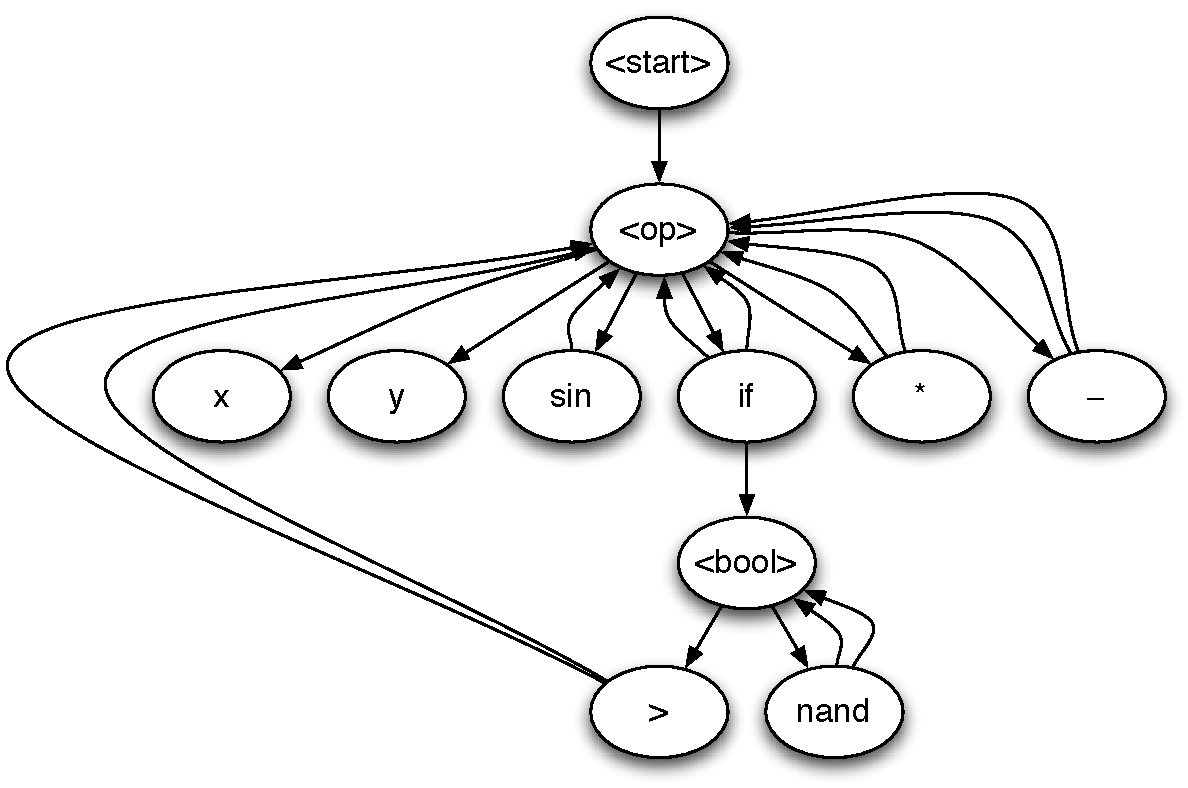
\includegraphics[width=4in]{ge.pdf}
\end{center}
\caption{Parse graph (orderings among children not shown). The entry point is {\tt \(<\)start\(>\)}.  GrammarRuleNodes are shown with angle brackets.  GrammarFunctionNodes are shown without brackets.}
\label{geparsegraph}
\end{figure}


\subsection{How Parsing is Done}

GESpecies parses the grammar files by running them through an \class{ec.gp.ge.GrammarParser}, a special class which converts the files into parse graphs.  The parse graphs consist of two kinds of nodes: a \class{ec.gp.ge.GrammarFunctionNode} and a \class{ec.gp.ge.GrammarRuleNode}, both subclasses of the abstract class \class{ec.gp.ge.GrammarNode}.  You can replace \class{ec.gp.ge.GrammarParser} with your own subclass if you like, via:


\params{%
pop.subpop.0.species.parser = ec.app.MySpecialGrammarParser
}

The parse graph produced by a GrammarParser is rooted with a GrammarRuleNode which indicates the initial rule.   For example, reconsider the grammar below.

\vbox{\small\begin{verbatim}
<start> ::= <op>
<op> ::= (x) | (y) | (sin <op>) | (* <op> <op>) | (- <op> <op>)
<op> ::= (if <bool> <op> <op>)
<bool> ::= (nand <bool> <bool>)
<bool> ::= (> <op> <op>)
\end{verbatim}}

The parse graph for this grammar is shown in Figure \ref{geparsegraph}.  Once the parse graph has been generated, the GESpecies wanders through this graph as follows:

\begin{itemize}
\item If on a GrammarRuleNode, the GESpecies selects exactly one child to traverse, using the next number in the GEIndividual array.
\item If on a GrammarFunctionNode, the GESpecies traverses each and every child of the node in order.  These become children to the GrammarFunctionNode's GPNode.
\end{itemize}

GrammarFunctionNodes hold GPNode prototypes and represent them.   Their children are arguments to the node in question. GrammarRuleNodes hold choice points in the rule, and their children are the choices (only one choice will be made).





\section{Rulesets and Collections (The \package{ec.rule} Package)}

Let's get one thing out of the way right now.  Though we had rulesets in mind when we developed it, the \package{ec.rule} package isn't {\it really} for rulesets.  Not only can the package be used for things other than rules, but it's not even sets: it's {\it collections} (or ``bags'' or ``multisets'') of arbitrary objects.  

The representation defined by this package is fairly straightforward: an \class{ec.rule.RuleIndividual} contains one or more \class{ec.ruleRuleSet}s, each of which contain zero or more \class{ec.rule.Rule}s.  A Rule is an abstract superclass which can contain anything you want.  And that's about it.

Problem domains for which the \package{ec.rule} package is appropriate are often also good candidates for the variable-length lists found in the \package{ec.vector} package.  You'll need to think about which is a better choice for you.  Also beware that of the various representation packages in ECJ, \package{ec.rule} is definitely the least used and least tested.  So its facilities are somewhat cruder than the others and it's possible you may see bugs.

Each level of the \package{ec.rule} package (individual, ruleset, rule) is a Prototype and has a Flyweight relationship with a central object special to that level (for a reminder on Flyweights, see Section~\ref{flyweight}).  Specifically:

{
\begin{center}
\small
\renewcommand{\arraystretch}{1.2} 
\begin{tabular}{r|l}
{\bf Object}&{\bf In Flyweight Relationship With}\bstrut\\
\hline\tstrut
\class{ec.rule.RuleIndividual}&\class{ec.rule.RuleSpecies}\\
\class{ec.rule.RuleSet}&\class{ec.rule.RuleSetConstraints}\\
\class{ec.rule.Rule}&\class{ec.rule.RuleConstraints}
\end{tabular}
\end{center}
}

The \package{ec.rule} package follows the same approach as the \package{ec.vector} package does when it comes to breeding: two basic breeding operators are provided (\class{ec.rule.breed.RuleCrossoverPipeline} and \class{ec.rule.breed.RuleMutationPipeline}) which simply call default mutation and crossover functions in the Individuals themselves.  Thus to do more sophisticated breeding you have the choice of either overriding these functions or creating new breeding pipelines which perform more detailed operations on their own.

\subsection{RuleIndividuals and RuleSpecies}  RuleIndividuals and RuleSpecies are specified in parameters in the standard way:

\params{%
pop.subpop.0.species = ec.rule.RuleSpecies\\
pop.subpop.0.species.ind = ec.rule.RuleIndividual
}

A RuleIndividual is a subclass of Individual which simply consists of an array of RuleSets:

\java{%
    public RuleSet[] rulesets;
}

Each RuleSet can be a different class.  You'd think that the number and class of RuleSets was specified in the RuleSpecies (like in \package{ec.vector}).  But for no good reason it's not the case: you specify them in the parameters for the prototypical individual, along these lines:

\params{%
pop.subpop.0.species.ind.num-rulesets = 2\\
pop.subpop.0.species.ind.ruleset.0 = ec.rule.Ruleset\\
pop.subpop.0.species.ind.ruleset.1 = ec.app.myapp.MyRuleset
}

Alternatively, you can use the RuleIndividual's default parameter base:

\params{%
rule.individual.num-rulesets = 2\\
rule.individual.ruleset.0 = ec.rule.Ruleset\\
rule.individual.ruleset.1 = ec.app.myapp.MyRuleset
}

Though for many applications you will probably just have a single RuleSet, and it'll probably just be an \class{ec.rule.Ruleset}:

 \params{%
pop.subpop.0.species.ind.num-rulesets = 1\\
pop.subpop.0.species.ind.ruleset.0 = ec.rule.Ruleset
}



\subsection{RuleSets and RuleSetConstraints}
\label{ec.rule.RuleSet}
\label{ec.rule.RuleSetConstraints}

A RuleSet contains an arbitrary number of Rules (\class{ec.rule.Rule}), anywhere between zero and up.  It's largely your job to customize the breeding and initialization procedures appropriate to your problem to constraint the number and type of rules.  They're defined here:

\java{%
    public Rule[] rules;\\
    public int numRules;
}

Notice that the number of rules in the array may be {\it less} than the array size, that is, \variable{numRules \(\leq\) rules.length}.  The rules themselves run from \variable{rules[0] ... rules[numRules \(-\) 1]}.  This is done because, like ArrayList etc.,  \variable{rules} is variable in size and an grow and shrink.  RuleSet contains a number of utility methods for manipulating the order and number of these rules:

\begin{methods}{ec.rule.RuleSet}
\mthd{public int numRules()}
Returns the number of rules in the RuleSet.
\mthd{public void randomizeRulesOrder(EvolutionState \textit{state}, int thread)}
An auxillary debugging method which verifies many features of the structure of the GPTree and all of its GPNodes.  This method isn't called by ECJ but has proven useful in determining errors in GPTree construction by various tree building or breeding algorithms.
\mthd{public void addRule(Rule \textit{rule})}
Adds the rule to the end of the ruleset, increasing the length of the RuleSet array as necessary.
\mthd{public void addRandomRule(EvolutionState \textit{state}, int thread)}
Produces a new randomly-generated rule and adds it to the RuleSet.  The Rule is created by cloning the prototypical Rule from the RuleSet's RuleSetConstraints, then calling reset(...) on it.
\mthd{public Rule removeRule(int \textit{index})}
Removes a rule located at the given index from the RuleSet and returns it.  All rules are shifted down to fill the void.
\mthd{public Rule removeRandomRule(EvolutionState \textit{state}, int thread)}
Removes a random rule returns it.  All rules are shifted down to fill the void.
\mthd{public RuleSet[] split(int[] \textit{points}, RuleSet[] \textit{sets})}
Breaks the RuleSet into \(n\) disjoint groups, then clones the rules in those groups and adds them to the respective sets, which must be provided in the given array.  The first group of rules starts at 0 and ends below \variable{points[0]}: this goes into \variable{sets[0]}. Intermediate groups, which go into \variable{sets[i]}, start at \variable{points[i]} and end below \variable{points[i+1]}.  The final group, which goes into \variable{sets[points.length]}, starts at \variable{points[points.length \(-\) 1]} and continues to the end of the rule array.  If \variable{points.length = 0}, then all rules simply get put into \variable{sets[0]}.  Note that the size of \variable{sets} must be one more than the size of \variable{points}.  The sets are returned.
\mthd{public RuleSet[] split(EvolutionState \textit{state}, int \textit{thread}, RuleSet[] {\it sets})}
For each rule in the RuleSet, clones the rule and adds the clone to a randomly chosen RuleSet from \variable{sets}.  Returns \variable{sets}.
\mthd{public RuleSet[] splitIntoTwo(EvolutionState \textit{state}, int \textit{thread}, RuleSet[] {\it sets}, float {\it probability})}
For each rule in the RuleSet, clones the rule and, with the given probability, adds the clone to \variable{sets[0]}, else \variable{sets[1]}.  Note that \variable{sets} must be two in length.
\mthd{public void join(RuleSet \textit{other})}
Copies the rules in the other RuleSet, then adds them to the end of this RuleSet.
\mthd{public void copyNoClone(RuleSet \textit{other})}
Deletes all the rules in the RuleSet.  Then places all the rules from the other RuleSet into this RuleSet.  No cloning is done: both RuleSets now have pointers to the same rules.
\end{methods}

Groups of RuleSets have a flyweight relationship with a RuleSetConstraints object.  RuleSetConstraints is a Clique.  You specify the number and class of RuleSetConstraints and assign each a unique name.  Let's say you need two RuleSetConstraints objects, both instances of RuleSetConstraints itself.  You'd write this:

\params{%
rule.rsc.size = 2\\
rule.rsc.0 = ec.rule.RuleSetConstraints\\
rule.rsc.0.name = rsc1\\
rule.rsc.1 = ec.rule.RuleSetConstraints\\
rule.rsc.0.name = rsc2
}

RuleSetConstraints specify a number of constraints which guide the initialization and mutation of  RuleSets, specifically:

\begin{itemize}
\item A distribution for choosing the number of Rules an initial RuleSet will have.  This guides how the RuleSet's \method{reset(...)} method operates.  The distribution can either be uniform with a minimum and maximum, or you can specify a histogram of possible size probabilities.  We'll do the first case for Ruleset 0 and the second case for Ruleset 1 below:

\params{%
\# RuleSetConstraints 0 will have between 5 and 10 rules inclusive\\
rule.rsc.0.reset-min-size = 5\\
rule.rsc.0.reset-min-size = 10\\
\\
\# RuleSetConstraints 1 will have 0 to 4 rules with these probabilities...\\
rule.rsc.1.reset-num-sizes = 5\\
rule.rsc.1.size.0 = 0.1\\
rule.rsc.1.size.1 = 0.2\\
rule.rsc.1.size.2 = 0.2\\
rule.rsc.1.size.3 = 0.3\\
rule.rsc.1.size.4 = 0.4
}

\item The probability of adding, deleting, and rearranging rules, when the RuleSet's \method{mutate(...)} method is called, typically by the BreedingPipeline \class{ec.rule.RuleMutationPipeline}.  When this method is called, the Ruleset first mutates all of its rules by calling \method{mutate(...)} on them.  Then it repeatedly flips a coin of a given probability: each time the coin comes up true, or until the number of rules is equal to the minimum number of initial rules as specified above,  one rule is deleted.  Afterwards it repeatedly flips a coin of another probability: each time the coin comes up true, or until the number of rules is equal to the maximum number of initial rules, one new rule is added at random.  Finally, with a certain probability the rule ordering is shuffled.  Here's some examples of specifying these probabilities:

\params{%
rule.rsc.0.p-add = 0.1\\
rule.rsc.0.p-del = 0.1\\
rule.rsc.0.rand-order = 0.25\\
\\
rule.rsc.1.p-add = 0.5\\
rule.rsc.1.p-del = 0.6\\
rule.rsc.1.rand-order = 0.0
}
\end{itemize}

Once you've specified a RuleSetConstraints, you then attach one to each RuleSet.  For example:

\params{%
pop.subpop.0.species.ind.ruleset.0.constraints = rsc2\\
pop.subpop.0.species.ind.ruleset.1.constraints = rsc1
}

\noindent ... or alternatively use the default parameter base...

\params{%
rule.individual.constraints = rsc2
}

Once set, you can access the constraints with the following method:

\begin{methods}{ec.rule.RuleSet}
\mthd{public final RuleSetConstraints ruleSetConstraints(RuleInitializer {\it initializer})}
Returns the RuleSet's RuleSetConstraints
\end{methods}

RuleSetConstraints one method for choosing random initial values under the constraints above:

\begin{methods}{ec.rule.RuleSetConstraints}
\mthd{public int numRulesForReset(RuleSet {\it ruleset}, EvolutionState {\it state}, int {\it thread})}
Returns a random value from the initial (\method{reset(...)}) distribution, to use as the number of rules to initialize or reset the RuleSet.
\end{methods}

Additionally, the various addition, deletion, and randomization probabilities can be accessed like this:

\java{%
RuleSetConstraints rsc = myRuleSet.ruleSetConstraints((RuleInitializer)(state.init));\\
float addition = rsc.p\_add;\\
float deletion = rsc.p\_del;\\
float shuffling = rsc.p\_randorder;
}

RuleSets also contain all the standard reading and writing methods, none of which you'll need to override unless you're making a custom RuleSet.

\begin{methods}{ec.rule.RuleSet}
\mthd{public void printRuleSetForHumans(EvolutionState {\it state}, int {\it log})}
Writes a RuleSet to a log in a fashion easy for humans to read.
\mthd{public void printRuleSet(EvolutionState {\it state}, int {\it log})}
Writes a RuleSet to a log in a fashion that can be read back in via readRule(...), typically by using the Code package.
\mthd{public void printRuleSet(EvolutionState {\it state}, PrintWriter {\it writer})}
Writes a RuleSet to a Writer in a fashion that can be read back in via readRule(...), typically by using the code package.
\mthd{public void readRuleSet(EvolutionState {\it state}, LineNumberReader {\it reader}) throws IOException}
Reads a RuleSet written by \method{printRuleSet(...)} or \method{printRuleSetToString(...)}, typically using the Code package. \mthd{public void writeRuleSet(EvolutionState {\it state}, DataOutput {\it output}) throws IOException}
Writes a RuleSet in binary fashion to the given output.
\mthd{public void readRuleSet(EvolutionState {\it state}, DataInput {\it input}) throws IOException}
Reads a RuleSet in binary fashion from the given input.
\end{methods}


\subsection{Rules and RuleConstraints}

RuleSetConstraints also contain the {\bf prototypical Rule} for RuleSets adhering to a given constraints.  RuleSets will clone this Rule to create Rules to fill themselves with.  \class{ec.rule.Rule} is an abstract superclass which doesn't do anything by itself: you're required to subclass it to make the Rule into the kind of thing you want to create a collection of in your Ruleset.

The prototypical Rule is specified like this:

\params{%
pop.subpop.0.species.ind.ruleset.0.rule = ec.app.MyRule\\
pop.subpop.0.species.ind.ruleset.1.rule = ec.app.MyOtherRule
}

You can get the prototypical rule like this:

\java{%
RuleSetConstraints rsc = myRuleSet.ruleSetConstraints((RuleInitializer)(state.init));\\
Rule prototype = rsc.rulePrototype;
}

Each Rule has a flyweight-related RuleConstraints object, which is defined similarly to RuleSetConstraints (it's also a Clique).  For example, to create a single RuleConstraints in the clique, you might say:

\params{%
rule.rc.size = 1\\
rule.rc.0 = ec.rule.RuleConstraints\\
rule.rc.0.name = rc1
}

RuleConstraints are essentially blank: they define no special parameters or variables.  You can use them however you see fit.  If you don't really care, you can just make a single RuleConstraints object as above and assign it to your prototypical rules, such as:

\params{%
pop.subpop.0.species.ind.ruleset.0.rule.constraints = rc1\\
pop.subpop.0.species.ind.ruleset.1.rule.constraints = rc1
}

\noindent ...or use the default parameter base:

\params{%
rule.rule.constraints = rc1
}

A Rule is abstract, and so has certain abstract methods which must be overridden, as well as others which {\it ought} to be overridden.  First the required ones:

\begin{methods}{ec.rule.Rule}
\mthd{public abstract int hashCode()}
Returns a hash code for the rule, based on value, suitable for weeding out duplicates.
\mthd{public abstract int compareTo(Object {\it other})}
Returns 0 if this Rule is identical in value to {\it other} (which will also be a Rule), -1 if this Rule is ``less'' than the other rule in sorting order, and 1 if the Rule is ``greater'' than the other rule in sorting order.
\mthd{public abstract void reset(EvolutionState {\it state}, int {\it thread})}
Randomizes the value of the rule.
\end{methods}

Rules are Prototypes and so implement the \method{clone()}, \method{setup(...)}, and \method{defaultBase()} methods.  You'll most likely need to override the \method{clone()} and \method{setup(...)} methods as usual.  Additionally, you may want to override:

\begin{methods}{ec.rule.Rule}
\mthd{public void mutate(EvolutionState {\it state}, int {\it thread})}
Mutates the Rule in some way and with some probability.  The default implementation simply calls \method{reset(...)}, which is probably much too harsh.
\mthd{public abstract int compareTo(Object {\it other})}
Returns 0 if this Rule is identical in value to {\it other} (which will also be a Rule), -1 if this Rule is ``less'' than the other rule in sorting order, and 1 if the Rule is ``greater'' than the other rule in sorting order.
\mthd{public abstract void reset(EvolutionState state, int thread)}
Randomizes the value of the rule.
\end{methods}


Then there are the standard printing and reading methods.  You'll need to override at least \method{printRuleToStringForHumans()}, and probably will want to override \method{toString()}.  The others you can optionally override depending on the kind of experiments you're doing.

\begin{methods}{ec.rule.Rule}
\mthd{public String toString()}
Writes the Rule to a String, typically in a fashion that can be read back in via readRule(...).  You'll want to override this method or \method{printRuleToString()}.  You probably want to use the Code package to write the rule out.    You only really need to implement this method if you expect to write Individuals to files that will be read back in later.
\mthd{public String printRuleToStringForHumans()}
Writes the Rule to a String in a fashion easy for humans to read.  The default implementation of this method simply calls toString().  You'll probably want to override this method.
\mthd{public void printRuleForHumans(EvolutionState {\it state}, int {\it log})}
Writes a Rule to a log in a fashion easy for humans to read.  The default implementation of this method calls \method{printRuleToStringForHumans()}, which you should probably override instead.
\mthd{public String printRuleToString()}
Writes the Rule to a String, typically in a fashion that can be read back in via readRule(...).  The default implementation of this method simply calls toString().   You'll want to override this method or \method{toString()}.    You probably want to use the Code package to write the rule out.  You only need to implement this method if you expect to write Individuals to files that will be read back in later.
\mthd{public void printRule(EvolutionState {\it state}, int {\it log})}
Writes a Rule to a log in a fashion that can be read back in via readRule(...).  The default implementation of this method calls \method{printRuleToString()}, which you should probably override instead.
\mthd{public void printRule(EvolutionState {\it state}, PrintWriter {\it writer})}
Writes a Rule to a Writer in a fashion that can be read back in via readRule(...).  The default implementation of this method calls \method{printRuleToString()}, which you should probably override instead.
\mthd{public void readRule(EvolutionState {\it state}, LineNumberReader {\it reader}) throws IOException}
Reads a Rule written by \method{printRule(...)} or \method{printRuleToString(...)}, typically using the Code package.  The default does nothing.  You only need to implement this method if you expect to read Individuals from files.
\mthd{public void writeRule(EvolutionState {\it state}, DataOutput {\it output}) throws IOException}
Writes a Rule in binary fashion to the given output.  The default does nothing.  You only need to implement this method if you expect to read and write Rules over a network (such as the distributed evaluation or island models).
\mthd{public void readRule(EvolutionState {\it state}, DataInput {\it input}) throws IOException}
Reads a Rule in binary fashion from the given input.  The default signals an error.  You only need to implement this method if you expect to read and write Rules over a network (such as the distributed evaluation or island models).
\end{methods}

\subsection{Initialization}

Basic Initialization works as follows:

\begin{enumerate}
\item The RuleSpecies method \method{newIndividual(EvolutionState, int)} produces a RuleIndividual by calling \method{super.newIndividual(...)}\,---\,cloning a RuleIndividual prototype\.---\,and then calling \method{reset(...)} on the resultant RuleIndividual.

\item The RuleIndividual's \method{reset(...)} by default just calls \method{reset(...)} on each of the RuleSets.

\item A RuleSet's \method{reset(...)} method calls \method{numRulesForReset(...)} on the RuleSetConstraints to pick a random number of rules to generate (see Section \ref{ec.rule.RuleSetConstraints}).  It then produces an array of that size and fills it with rules cloned from the RuleSetConstraint's prototypical Rule.  Then it calls \method{reset(...)} on each of the Rules.

\item You are responsible for implementing a Rule's \method{reset(...)} method.
\end{enumerate}

You can of course intervene and modify any of these methods as you see fit.

\subsection{Mutation}

As in the case in the \package{ec.vector} package, the \class{ec.rule.breed.RuleMutationPipeline} class doesn't mutate rules directly, but rather calls a method on them to ask them to mutate themselves.  The procedure is as follows:

\begin{enumerate}
\item The RuleMutationPipeline calls \method{preprocessIndividual(...)} on the RuleIndividual.

\item The RuleIndividual's \method{preprocessIndividual(...)} method calls \method{preprocessRules(...)} on each of the RuleSets.

\item The RuleSet's \method{preprocessRules(...)} method by default does nothing: override it as you like.

\item The RuleMutationPipeline then calls \method{mutate(...)} on the RuleIndividual.

\item The RuleIndividual's \method{mutate(...)} method by default just calls \method{mutate(...)} on each of its RuleSets.

\item The RuleSet's \method{mutate(...)} method does several modifications to the rules in the RuleSet, in this order:

\begin{enumerate}

\item All the Rules in the RuleSet have \method{mutate(...)} called on them.

\item A coin of is repeatedly flipped of a certain probability (\variable{p\_del}), and each time it comes up true, a rule is deleted at random using \method{removeRandomRule(...)}.  The indivdiual will not shrink smaller than its specified minimum size.

\item A coin of is repeatedly flipped of a certain probability (\variable{p\_add}), and each time it comes up true, a rule is added at random using \method{addRandomRule(...)}.  That method clones a new Rule from the prototypical Rule, then calls \method{reset(...)} on it.  The indivdiual will not grow larger than its specified maximum size.

\item With a certain  probability (\variable{p\_randorder}), the order of the rules is shuffled using \method{randomizeRulesOrder(...)}.

\end{enumerate}

The three probabilities (\variable{p\_del}, \variable{p\_add}, and \variable{p\_randorder}), and the minimum and maximum rule sizes, are discussed in Section \ref{ec.rule.RuleSet}, and are determined by RuleSetConstraints parameters, also discussed in that Section.

\item A Rule's \method{mutate(...)} method by default simply calls \method{reset(...)}, which is probably not what you want.  You'll probably want a much more subtle mutation if any, and so will need to override this method.

\item You are responsible for implementing a Rule's \method{reset(...)} method.

\item Finally, the RuleMutationPipeline calls \method{postprocessIndividual(...)} on the RuleIndividual.

\item The RuleIndividual's \method{postprocessIndividual(...)} method calls \method{postprocessRules(...)} on each of the RuleSets.

\item The RuleSet's \method{postprocessRules(...)} method by default does nothing: override it as you like.

\end{enumerate}

Often rules need to be in a carefully-constructed dance of constraints to be valid in an Individual.  The intent of the \method{preprocessIndividual(...)}, \method{postprocessIndividual(...)}, \method{preprocessRules(...)}, and \method{postProcessRules(...)} methods is to give your RuleIndividual a chance to fix RuleSets that have been broken by crossover or mutation.  The default implementation of these methods doesn't do much:

\begin{methods}{ec.rule.RuleSet}
\mthd{public void preprocessRules(EvolutionState {\it state}, int {\it thread})}
A hook called prior to mutation or crossover to prepare for possible breakage of Rules due to the mutation or crossover event.  The default implementation does nothing.
\mthd{public void postprocessRules(EvolutionState {\it state}, int {\it thread})}
A hook called after to mutation or crossover to fix possible breakage of Rules due to the mutation or crossover event.  The default implementation does nothing.
\end{methods}

\begin{methods}{ec.rule.RuleIndividual}
\mthd{public void preprocessIndividual(EvolutionState {\it state}, int {\it thread})}
Calls preprocessRules(...) on each RuleSet in the Individual.
\mthd{public void postprocessIndividual(EvolutionState {\it state}, int {\it thread})}
Calls postprocessRules(...) on each RuleSet in the Individual.
\end{methods}




\subsection{Crossover}

Unlike RuleMutationPipeline, the \class{ec.rule.breed.RuleCrossoverPipeline} performs direct crossover on two RuleIndividuals.  Here is the procedure:

\begin{enumerate}
\item The RuleCrossoverPipeline calls \method{preprocessIndividual(...)} on each RuleIndividual.

\item The RuleIndividual's \method{preprocessIndividual(...)} method calls \method{preprocessRules(...)} on each of the RuleSets.

\item The RuleSet's \method{preprocessRules(...)} method by default does nothing: override it as you like.

\item For each pair of RuleSets, one per RuleIndividual...

\begin{enumerate}

\item Each RuleSet \(A\) and \(B\) is split into two pieces, \(A_1\) and \(A_2\) (and \(B_1\) and \(B_2\)) by calling \method{splitIntoTwo(...)}
\item A new RuleSet \(A'\) is formed from the union of \(A_1\) and \(B_1\), and likewise, a new RuleSet \(B'\) is formed from the union of \(A_2\) and \(B_2\).
\item If \(A'\) and \(B'\) do not minimum and maximum size constraints (see Section \ref{ec.rule.RuleSetConstraints}), go to (a) and try again.
\item Else \(A'\) and \(B'\) replace \(A\) and \(B\) respectively in each RuleIndivdiual.

\end{enumerate}

\item Finally, the RuleCrossoverPipeline calls \method{postprocessIndividual(...)} on each RuleIndividual.

\item The RuleIndividual's \method{postprocessIndividual(...)} method calls \method{postprocessRules(...)} on each of the RuleSets.

\item The RuleSet's \method{postprocessRules(...)} method by default does nothing: override it as you like.

\end{enumerate}

RuleCrossoverPipeline has a few parameters which guide its operation.   First, any given Rule will migrate from one Individual's RuleSet to the other only with a certain probability.  Second, the CrossoverPipeline can be set up to return only one child (tossing the second) rather than returning two.  By default it returns both children.  To set both of these parameters, let's say that the RuleCrossoverPipeline is the root pipeline for the species.  We'd say:

\params{%
pop.subpop.0.species.pipe = ec.rule.breed.RuleCrossoverPipeline\\
pop.subpop.0.species.pipe.crossover-prob = 0.1\\
pop.subpop.0.species.pipe.toss = true
}

It doesn't make any sense to have a rule crossover probability higher than 0.5.  As usual, you could use the default parameter base as well:

\params{%
rule.xover.crossover-prob = 0.1\\
rule.xover.toss = true
}


















\chapter{Parallel Processes}

ECJ has various built-in methods for parallelism, and they can be used in combination with one another:

\begin{itemize}
\item Multiple breeding and evaluation {\bf threads}, already discussed in Section \ref{threads}.
\item {\bf Distributed evaluation}: sending chunks of Individuals to remote computers to be evaluated.   This is typically done in a generational fashion, but a variation of this is {\bf asynchronous evolution}, in which Individuals are sent to multiple remote computers in a steady-state fashion.  Additionally, remote computers can (given time) engage in a little evolutionary optimization of their own on the chunks they've received before sending them back.  This is known as {\bf opportunistic evolution}.\footnote{ECJ's built-in distributed evaluation is meant for clusters.  However, Parabon Inc. has developed a grid-computing version, called Origin, which runs on hundreds of thousands or even millions of machines.  See the ECJ main website for more information.}
\item {\bf Island models}: multiple parallel evolutionary processes occasionally send fit individuals to one another.\footnote{ECJ's built-in island models are meant for clusters.  However, a version of ECJ was ported to run on top of the DR-EA-M system, a peer-to-peer evolutionary computation network facility developed from a grant in Europe. See the ECJ main website for more information.}
\end{itemize} 


\begin{figure}[t]
\begin{center}
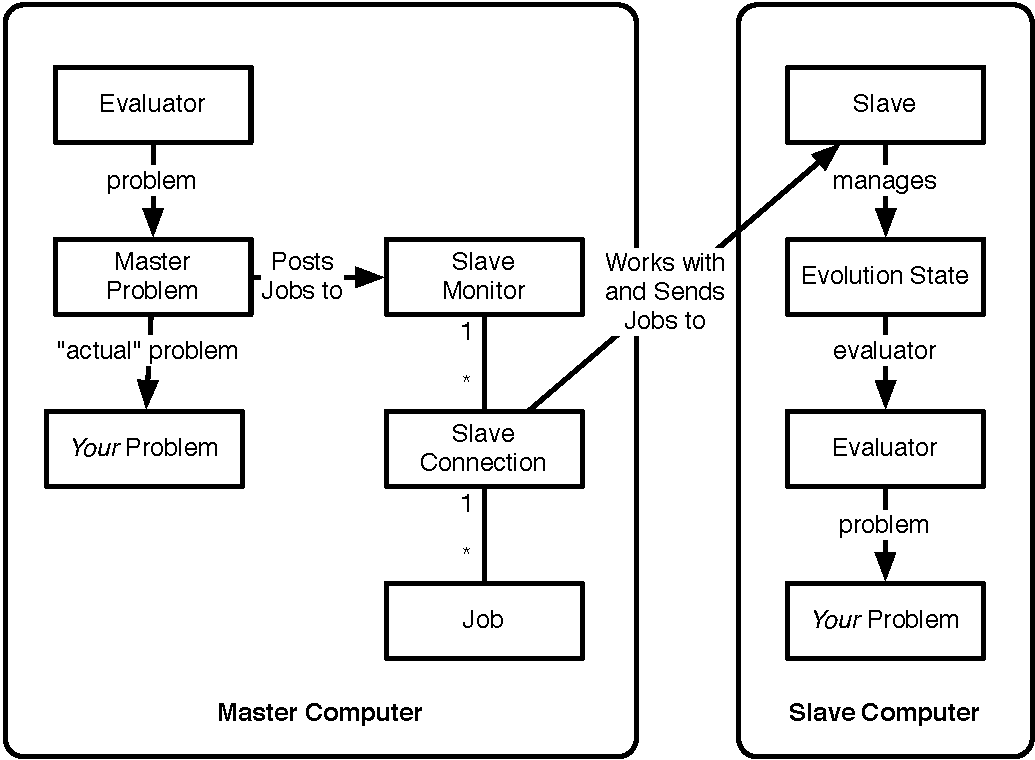
\includegraphics[width=4in]{Distributed.pdf}
\end{center}
\caption{Layout of the Distributed Evaluation package.}
\label{DistributedEvaluation}
\end{figure}

\section{Distributed Evaluation (The \package{ec.eval} Package)}
\label{ec.eval}

Distributed Evaluation is connects one {\bf master} ECJ process with some \(N\) {\bf slave} ECJ processes.  The master handles the evolutionary loop, but when Individuals are evaluated, they are shipped off to the remote slaves to do this task.  This way evaluation can be parallelized.


Distributed Evaluation is only useful if the amount of time you save by parallelizing evaluation exceeds the amount of time lost by shipping Individuals over the network (and sending at least Fitnesses back).  Generally this means that evaluation needs to take a fair bit of time per Individual: perhaps several seconds.

There are two kinds of EvolutionState objects which can work with Distributed Evaluation:

\begin{itemize}
\item SimpleEvolutionState, which sends entire Populations off to be evaluated in parallel.
\item SteadyStateEvolutionState, which sends individuals off to be evaluated one at a time, in a fashion called {\bf asynchronous evolution}.
\end{itemize}

\subsection{The Master}

To set up Distributed Evaluation, you first need to set up the Master.  This is done just like a regular evolutionary computation process: but there are some additional parameters which must be defined.  First, we must define the {\bf master problem}, nearly always as \class{ec.eval.MasterProblem}.  The presence of the master problem turns on distributed evaluation:

\params{%
eval.masterproblem = ec.eval.MasterProblem
}

The MasterProblem is the interface that connects the distributed evaluation system to a regular evolutionary computation loop.  When it is defined, ECJ replaces the Problem prototype with a MasterProblem prototype  The Problem doesn't go away\,---\,it's rehung as a variable in the MasterProblem.  Specifically, you can get it like this:

\java{%
Problem originalProblem = ((MasterProblem)(state.evaluator.p\_problem)).problem;
}

When your evolutionary computation process  wishes to evaluate one or more individuals, it hands them to the MasterProblem, which it thinks is the Problem for the application.  But the MasterProblem doesn't send them to a clone of your underlying Problem but rather routes them to the Slave.  

Slaves register themselves over the network with an object in the Master process called a \class{ec.eval.SlaveMonitor}, which maintains one \class{ec.eval.SlaveConnection} per Slave to communicate with the remote Slave.  The SlaveMonitor listens in on a specific socket port for incoming Slaves to register themselves.  You'll need to define this port (to something over 2000).  Here's what's standard:

\java{%
eval.master.port = 15000
}


Your MasterProblem will submit Individuals to the SlaveMonitor, which will in turn direct them to one of the SlaveConnections.  SlaveConnections don't just ship of single Individuals to Slaves\,---\,that would be far too inefficient use of network bandwidth.  Instead, they often batch them up into {\bf jobs} for the Slave to perform.  Here's how you define the size of a job:

\java{%
eval.masterproblem.job-size = 100
}

The idea is to make the job large enough to pack Individuals into a network packet without wasting space.  If your Individuals are large, then a large job size won't have any efficiency benefit.  If they're very small, the job size will have a huge benefit.

You also need to keep the Slaves humming along, ideally by keeping the TCP/IP streams filled with waiting jobs queued up.  Increasing this number can have a significant effect on performance.  Here's a reasonable minumum:

\java{%
eval.masterproblem.max-jobs-per-slave = 3
}

ECJ would prefer to compress the network streams to make them more efficient.  But it can't do it without the jzlib/ZLIB library which you must install separately\footnote{Sure, Java has compression routines. Unfortunately they're entirely broken for network streams: they don't support ``partial flush'', a critical item for sending stuff across networks.  They're only really useful for compressing files on disks.} (see the ECJ main webpage or http:/\!/www.jcraft.com/jzlib).  Once it's installed, you can turn it on like this:

\java{%
eval.compression = true
}



\subsection{Slaves}

Slaves are started up on separate CPUs, often in different machines from the Master.  You can have as many Slaves as you like: the more the merrier.  The Slave class replaces \class{ec.Evolve} to handle its own startup, so you don't start up a Slave using the standard \class{ec.Evolve} procedure.  Instead you'd type:

\script{%
java ec.eval.Slave -file \textit{slave.params}
}

The slave parameters must include all the evolutionary parameters and also all the master parameters (in fact, you might as well say something like...)

\params{%
parent.0 = master.params
}

Slaves set themselves up with their own nearly complete EvolutionState and Evaluator objects\,---\,enough to evaluate Individuals and also perform evolution if necessary.  A slave distinguishes itself by setting a special internal parameter:  \parameter{eval.i-am-slave~=~true}.  You don't need to set this parameter\,---\,it's set programmatically by \class{ec.eval.Slave} when it's fired up.  But you should be aware of it: it's used by \class{ec.Evaluator} to determine whether to replace the Problem with the MasterProblem (it needs to know if the process is a Master or a Slave, and since your Slave probably included the Master parameters\,---\,including the \parameter{eval.masterproblem} parameter\,---\,it looks confusingly like a Master).

The first thing a Slave needs to know is where the Master is so it can set itself up.  This is done with something like this:

\params{%
eval.master.host = 129.8.2.4
}

Remember that you'll also need the port (among other Master parameters!)

Next the Slave needs to know whether it should return entire Individuals or just the Fitnesses of those Individuals.  Individuals are generally much bigger than Fitnesses, and if you only return Fitnesses you can cut your network traffic in half.  The problem is that in some custom experiments your fitness evaluation procedure might modify the Individual (it depends on the nature of your experiment).  You'll need to state whether to return entire Individuals or not:

\params{%
eval.return-inds = false
}

Slaves can come and go at any time dynamically.  If new slaves show up, the Master will immediately start taking advantage of them.  If a Slave disappears, the Individuals it was responsible for will be reassigned to another Slave.


\subsection{Opportunistic Evolution}

Slaves have the option of doing some evolutionary computation of their own, a procedure known as {\bf opportunistic evolution} \cite{opportunistic}.  The procedure works like this:

\begin{enumerate}
\item The Master sends the Slave a large Job.
\item The Slave evaluates the Individuals in the Job.
\item The Slave has a maximum allotted time to evaluate the Individuals.  If it has not yet exceeded this time, it treats the Job as a Population and does some evolution on the Slaves.
\item When the time is up, the Slave returns the most recent Individuals in the Population in lieu of the original Individuals.  The new Individuals replace the old ones in the Master's evolutionary process.  This means that the Slave cannot just return Fitnesses, but must return whole Individuals.
\end{enumerate}

This procedure is turned on with:

\params{%
eval.run-evolve = true
}

You'll also need to specify the amount of time (in milliseconds) allotted to the Slave.  Here's how you'd set it to six  seconds:

\params{%
eval.runtime = 6000
}

Last, if you're doing opportunistic evolution, you {\bf must} return whole Individuals, not just Fitnesses.  After all, you could have entirely different individuals after running on the Slave.  Thus you'll need to set:

\params{%
eval.return-inds = true
}

There's absolutely no reason the Slave can't have its own evolutionary algorithm that's {\it different} from the Master's evolutionary algorithm\,---\,just specify it differently in the Slave's parameters.  The only thing that'd be required is that the Slave and the Master have exactly the same kinds of Individuals, Fitnesses, and Species in their Subpopulations.

 Note that Opportunistic Evolution won't work with coevolution or other procedures which require GroupedProblemForm.  Additionally, although Steady-State Evolution (via Asynchronous Evolution, see Section \ref{asynchronous}) can work with Opportunistic Evolution in {\it theory}, it'd be quite odd to do so.

\begin{figure}[f]
\begin{center}
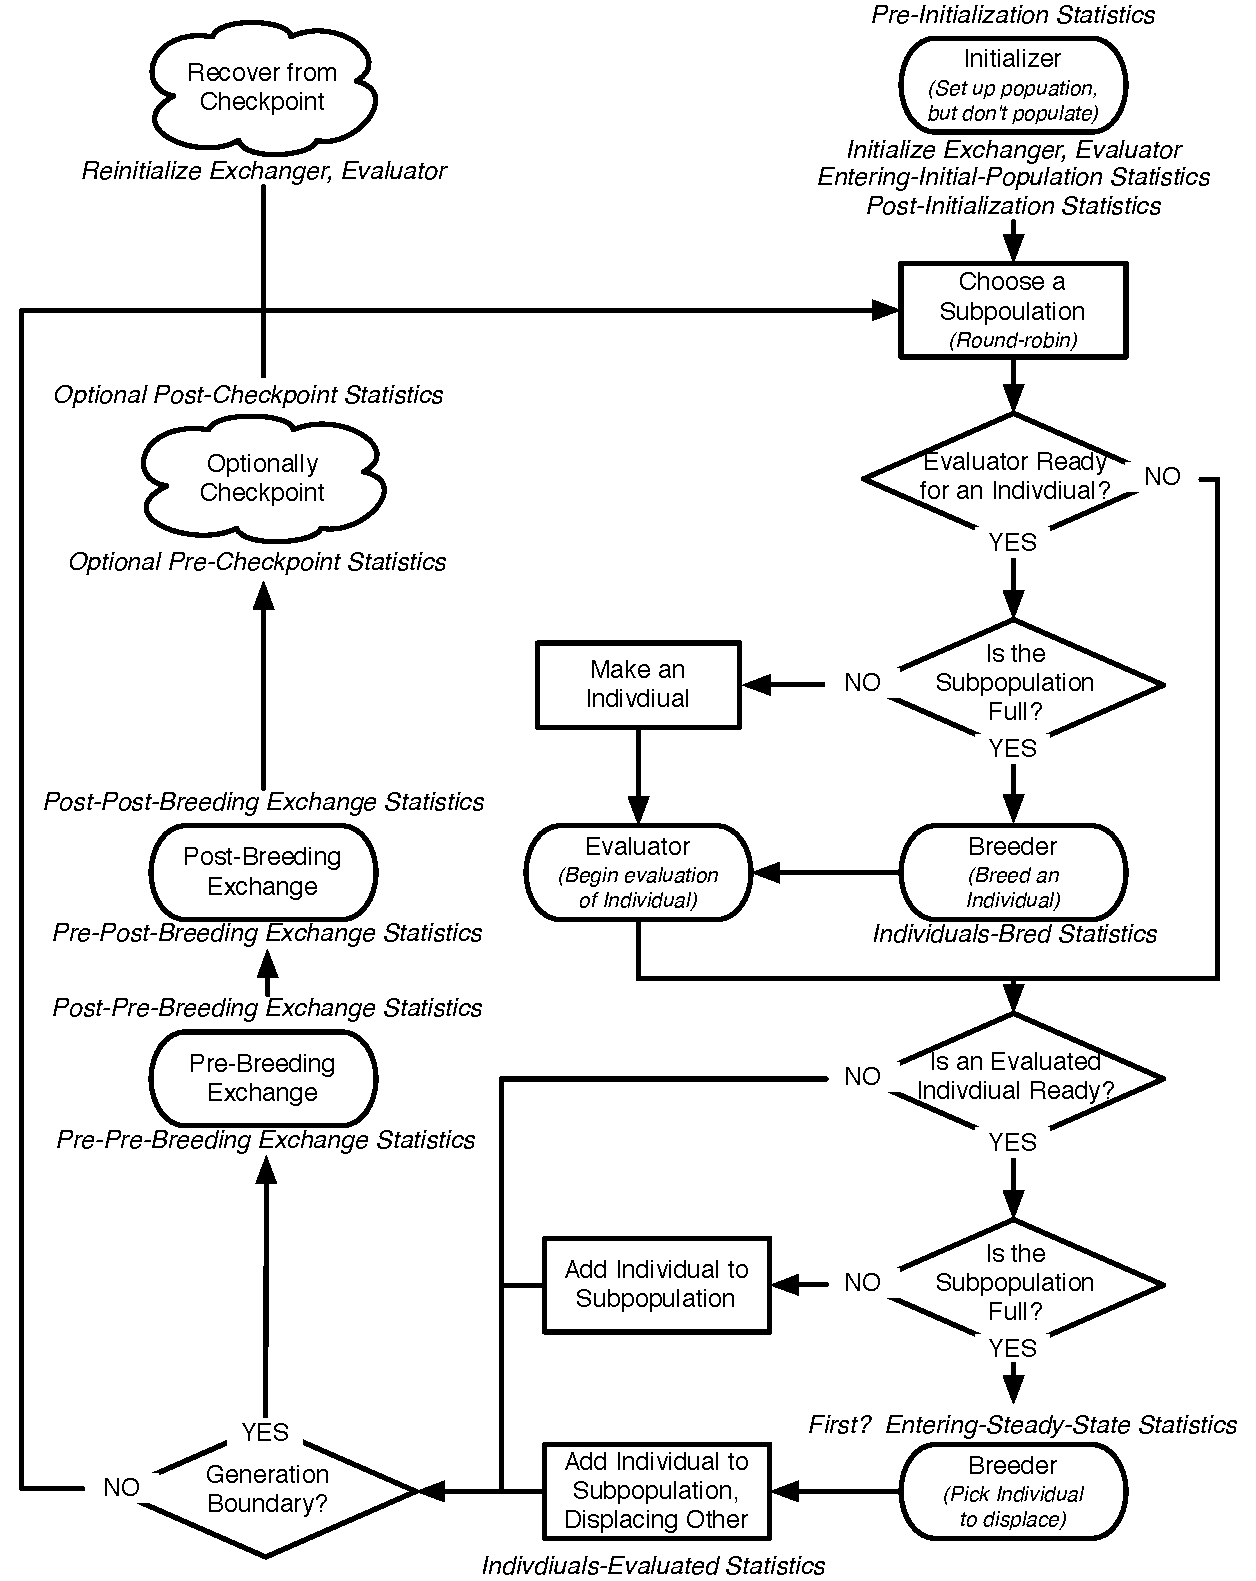
\includegraphics[height=7.5in]{SteadyState.pdf}
\end{center}
\caption{Top-Level Loop of ECJ's \class{SteadyStateEvolutionState} class, used for simple steady-state EC and Asynchronous Evolution algorithms.  {\it ``First?''} means to perform the Statistics whenever the Subpopulation in question is picking an Individual to displace for the very first time.  (Each Subpopulation will do it once, but possibly at different times).  A repeat of Figure \ref{SteadyState}.}
\label{AsynchronousEvolution}
\end{figure}
\afterpage{\clearpage}

\subsection{Asynchronous Evolution}
\label{asynchronous}

ECJ's distributed evaluation procedure works intuitively with generational methods (such as \class{ec.simple.SimpleEvolutionState} but it also works nicely with Steady-State evolution (\class{ec.simple.SteadyStateEvolutionState}).  This procedure is called {\bf asynchronous evolution}.  See \cite{opportunistic} for more information.

The procedure is similar to Steady State Evolution, as discussed in Section \ref{ec.steadystate}.  The Population starts initially empty.  Then the algorithm starts creating randomly-generated Individuals and shipping them off to remote Slaves to be evaluated.  If a Slave is available, the algorithm will generate an Individual for it to work on.  When a Slave has finished evaluating an Individual and has returned it (or its Fitness), the Individual is then placed into the Population.

At some point the Population will fill up.  At this point the algorithm shifts to ``steady state'' mode.  When a Slave returns an Individual, and there's no space in the Population, the algorithm makes room by marking an existing Individual for death and replacing it with the newcomer, just like it's done in Steady State Evolution.  And when a Slave becomes available, an Individual will no longer be created at random to give to it: rather, the Individual will be bred from the existing Population.

This procedure requires some careful consideration.  First, note that at the point that the algorithm shifts to ``steady state'' mode, there are probably a large number of Individuals being evaluated on Slaves which were not bred from the Population but were created at random.  Until those Individuals have made their way into the Population, we won't be in a true ``steady state''.

Second, Steady-State Evolution assumes the production of one Individual at a time: but distributed evaluation allows more than one individual per Job.  This is reconciled as follows.  when Steady-State Evolution starts up, it calls \method{prepareToEvaluate(...)} on the Problem (the MasterProblem) once.  Thereafter whenever an individual is sent to the Problem to be evaluated, it calls \method{evaluate(...)}.  Recall from Section \ref{ec.Problem} that this process does not require the Problem to immediately assign Fitness\,---\,it can bulk up Individuals for evaluation and is only required to provide Fitness on or prior to a call to \method{finishEvaluating(...)}.  However, Steady-State Evolution {\it never calls \method{finishEvaluating(...)}}.   As a result, the distributed evaluator is free to assess Individuals in any order and any way it likes, and take as long as it wishes to assign them a Fitness.  The distributed evaluator will wait for up to \parameter{job-size} worth of calls to \method{evaluate(...)}, then pack those Individuals together in one Job and ship them out to a remote Slave for evaluation.  In ``steady-state'' mode, when the Individuals come back, they are placed in the Population, killing and replacing other individuals already there.  Depending on the selection process for marking Individuals for death, it's entirely possible that an Individual newly placed into the Population may be immediately marked for death and replaced with another Individual from the same Job!  You can get around this by setting the \parameter{job-size} and \parameter{max-jobs-per-slave} to as low as 1:

\java{%
eval.masterproblem.job-size = 1\\
eval.masterproblem.max-jobs-per-slave = 1
}

\noindent ...but of course this will make the network utilization poor.

\subsection{The MasterProblem}
\label{ec.eval.MasterProblem}

The MasterProblem is where much of the magic lies in the interface between ECJ and the distributed evaluator, so it's worth mentioning some of its details.

To start, let's discuss how MasterProblem handles checkpointing.  Evaluators also three methods, which we didn't discuss in Section~\ref{ec.Evaluator}:

\java{%
public void initializeContacts(EvolutionState state);\\
public void reinitializeContacts(EvolutionState state);\\
public void closeContacts(EvolutionState state, int result);
}

These methods in turn call similar methods in the prototypical Problem:

\java{%
public void initializeContacts(EvolutionState state);\\
public void reinitializeContacts(EvolutionState state);\\
public void closeContacts(EvolutionState state, int result);
}

\variable{result} will be one of \variable{EvolutionState.R\_FAILURE} (the most common case) or \variable{EvolutionState.R\_SUCCESS} (which only happens if the Evaluator in this process or some external process found the ideal individual).

The default implementation of these Problem methods does nothing at all.  But in MasterProblem these methods are used to handle reconnection of Slaves after a checkpoint recovery.   The first two methods create both a new SlaveMonitor.  The final method shuts down the monitor cleanly.

MasterProblem also has special methods used only by Steady-State Evolution (and thus Asynchronous Evolution:

\begin{methods}{ec.eval.MasterProblem}
\mthd{public boolean canEvaluate()}
	Returns true if a Slave is available to take an Individual.
\mthd{public boolean evaluatedIndividualAvailable()}
	Returns true if a Slave has a completed Individual waiting to be introduced to the Population. 
\mthd{public QueueIndividual getNextEvaluatedIndividual()}
	Blocks until an Individual is available from a Slave.  Then returns it as an \class{ec.steadystate.QueueIndividual}.  A QueueIndividual is a very simple class which just contains the Individual and the Subpopulation that the Individual should be introduced into.  It has the following instance variables:
	
	\java{%
	public Individual ind;\\
	public int subpop;
	}
\end{methods}

MasterProblem also implements all the methods defined in SimpleProblemForm and GroupedProblemForm, in addition to the following two methods normally implemented by Evaluator (and which are called on the MasterProblem from the Evaluator's methods of the same names):

\begin{methods}{ec.eval.MasterProblem}
\mthd{public void prepareToEvaluate(EvolutionState {\it state}, int {\it threadnum})}
	Creates a new queue of Individuals who are out waiting to be sent to be processed.
\mthd{public void finishEvaluating(EvolutionState {\it state}, int {\it threadnum})}
	Sends all Individuals presently in the queue out in a Job.  Then waits for all slaves to complete evaluation of all Individuals.
\end{methods}


\section{Island Models (The \package{ec.exchange} Package)}
\label{ec.exchange}

In addition to Distributed Evaluation, ECJ supports Island Models: separate ECJ processes (``islands'') which connect over the network and occasionally hand highly-fit Individuals to one another.  This facility is handled by an Exchanger called \class{ec.exchange.IslandExchange} which ships individuals off to other islands immediately before breeding, and immediately after breeding brings in new individuals provided it by other islands.  You'll run your separate islands as ordinary processes.

Most of the issues in Island models surround the particular topology being chosen.  Which islands will send Individuals to which other islands?  How many at a time?  How often?  Are Individuals sent synchronously or asynchronously?  Etc.  ECJ manages all topology and connection parameters via a special ECJ process called the {\bf island model server}.  Each island will connect to and register itself with the server.  When the islands have all connected, the server will tell them which islands need to hook up to which other islands and how.  After the islands have hooked up, they're given the go-ahead to start their evolutionary processes.  If the islands are acting synchronously, each generation will wait for the server to give them the go-ahead to continue to the next generation; this go-ahead only occurs after all islands have finished the previous generation. Finally, when an island discovers an optimal individual, it will signal the server to let the other islands know (so they can shut down).

As you can see, the server really does little more than tell the islands how to connect and act as a referee.  Thus it's actually a very lightweight process.  You can run the server either as its own process like this:

\script{%
java ec.exchange.IslandExchange -file \textit{server.params} -p \textit{param=value} ... \hfill{\it (etc.)}
}

\noindent ...or an ECJ island can also do double-duty, serving as the server.  All islands, whether ordinary islands or double-duty island-server combos, are fired up in the same standard ECJ fashion:

\script{%
java ec.Evolve -file \textit{island.params} -p \textit{param=value} -p \textit{param=value} ... \hfill{\it (etc.)}
}

\noindent ...or (as usual):

\script{%
java ec.Evolve -checkpoint \textit{myCheckpointFile.gz}
}

A double-duty island-server combo would differ from a plain island solely in the parameters it defines: it'd need server parameters in addition to client parameters.

\paragraph{Mixing Island Models, Threading, and Distributed Evaluation}

There's absolutely no reason you create an unholy union of Island Models and Distributed Evaluation.  For example, it's perfectly reasonable to have an Island Model, where each island maintains its own pool of Slaves to do distributed evaluation.  It'd be a lot of parameter files though!  Island Models also work perfectly fine in a multithreaded environment.

\subsection{Islands}
\label{islands}

You set up an ECJ process as an island by defining a special Exchange object for it:

\params{%
exch = ec.exchange.IslandExchange
}

IslandExchange maintains the island's {\bf mailbox}.  Prior to breeding, the IslandExchange procedure will send some fit individuals off to mailboxes of remote islands.  The procedure for selecting Individuals is defined along these lines:

\params{%
exch.select = ec.select.TournamentSelection
}

After breeding, the IslandExchange will empty its own mailbox and introduce into the Population all of the Individuals contained therein.  These Individuals will displace some of the recently-bred Individuals, which never get a chance to be selected.\footnote{Life's not fair.}  The selection method for picking the Individuals to die and be displaced is defined as:

\params{%
exch.select-to-die = ec.select.RandomSelection
}

If this parameter isn't defined, individuals are picked at random.

An Island needs to know where the Server is so it can register itself, and the socket port on which the server is listening, for example:

\params{%
exch.server-addr = 128.2.30.4\\
exch.server-port = 8999
}

When an Island registers itself with the Server, it'll tell it two things.  First, it'll tell the Server the island's {\bf name}, a String which uniquely identifies the island (and by which the Server looks up topology information for the island).  Second, it'll tell the Server the socket port on which it'll receive incoming Individuals from other islands.  Let's say that you're creating an island called \variable{StatenIsland}.  You might specify the following:

\params{%
exch.id = StatenIsland\\
exch.client-port = 9002
}

Note that the client socket port should be (1) higher than 2000 and (2) different from other client ports, and the server port, if they're running on the same machine or in the same process.  You'll also probably want to have compressed network streams.  Like was the case in Distributed Evaluation, this can't be done without the jzlib/ZLIB library, which you must install separately (see the ECJ main webpage or http:/\!/www.jcraft.com/jzlib).  This is because Java's compression facilities are broken.  Once this library installed, you can turn it on like this:

\params{%
exch.compression = true
}

Be certain to give your island a unique random number seed different from other islands!  Don't set the seed to \parameter{time}, since it's possible that two islands will have the same seed because they were launched within the one millisecond of one another.  I'd hard-set the seed on a per-island basis.

\params{%
seed.0 = 5921623
}

If your islands share the same file system, you'll want to make sure they don't overwrite each other's statistics files etc.  To do this, for example, StatenIsland might change its statistics file name to:

\params{%
stat.file = \$statenisland.stat
}

If you have multiple Statistics files you'll need to change all of them; the same goes for other files being written out.  Also, if you are checkpointing, and your islands might overwrite each others' checkpoint files, you need to change the checkpoint prefix on a per-island basis.  For example:

\params{%
prefix = statenisland
}

Last, you can cut down on the verbosity of the islands by setting...

\params{%
exch.chatty = false
}

\subsection{The Server}

The Server holds all the parameters for setting up the island topology.  But first we must clue your ECJ process into realizing that it is a Server in the first place.  This is done with:

\params{%
exch.i-am-server = true
}

Next we need to state how many islands are in the island model graph:

\params{%
exch.num-islands = 3
}

As discussed in Section \ref{islands}, each island has a unique name (id).  Here you will state which island in your graph has which id:

\params{%
exch.island.0.id = StatenIsland\\
exch.island.1.id = ConeyIsland\\
exch.island.2.id = EllisIsland
}

Each island has some number of connections {\it to} other islands (the islands it'll send Individuals, or {\it migrants}, to).  In this example, we'll say that StatenIsland sends migrants to ConeyIsland, which sends migrants to EllisIsland, which sends migrants to both StatenIsland and ConeyIsland:


\params{%
exch.island.0.num-mig = 1\\
exch.island.0.mig.0 = ConeyIsland\\
exch.island.1.num-mig = 2\\
exch.island.1.mig.0 = EllisIsland\\
exch.island.2.num-mig = 2\\
exch.island.2.mig.0 = StatenIsland\\
exch.island.2.mig.1 = ConeyIsland
}

StatenIsland and ConeyIsland send 10 migrants to each of the islands they're connected to.  But we want EllisIsland to send 50 migrants to each of the (two) islands it's connected to:

\params{%
exch.island.0.size = 10\\
exch.island.1.size = 10\\
exch.island.2.size = 50
}

Altenatively you can use a default parameter base of sorts:

\params{%
exch.size = 10
}

Each island has a maximum mailbox capacity: if there is no room, further immigrants will be dropped and disappear into the ether.  You should make your mailbox big enough to accept immigrants at a reasonable rate, but not so large that in theory they could entirely overwhelm your population!  I suggest a mailbox three or four times the size of the expected immigrants.  How about 100 or 200?

\params{%
exch.island.0.mailbox-capacity = 200\\
exch.island.1.mailbox-capacity = 200\\
exch.island.2.mailbox-capacity = 200
}

Altenatively you can use a default parameter base of sorts:

\params{%
exch.mailbox-capacity = 10
}

Last you'll need to stipulate two additional parameters on a per-island basis: the {\bf start-generation} (in which generation the island will start sending Individuals out) and {\bf modulus} (how many generations the island will wait before it sends out another batch of Individuals).  These are mostly set to maximize network utilization: perhaps you may wish the islands to send out individuals at different times so as not to clog your network, for example.  Here we'll tell each island to send out individuals every three generations, but to start at different initial generations so to be somewhat staggered:

\params{%
exch.island.0.mod = 3\\
exch.island.1.mod = 3\\
exch.island.2.mod = 3\\
exch.island.0.start = 1\\
exch.island.1.start = 2\\
exch.island.2.start = 3
}

Altenatively you can use a default parameter base of sorts:

\params{%
exch.mod = 3\\
exch.start = 2
}




\subsubsection{Synchronicity}

Island models can be either {\bf synchronous} or {\bf asynchronous}.  In a synchronous island model, islands wait until they all have reached the next generation before sending immigrants to one another.  In the asynchronous island model, islands go at their own pace and send immigrants whenever they feel like it.  This means that one evolutionary process on one computer may run much faster than another one (good, because it doesn't waste resources waiting for the other one to catch up) but it may overwhelm the other process with multiple generations of immigrants before the other process can get around to processing them (usually bad).  Generally speaking asynchronicity is preferred\,---\,and is the default setting.

If for some reason you want to turn on synchronicity, you do this:

\params{%
exch.sync = true
}

Note that the modulo and start-generation of islands results in a predictable behavior for synchronous island models: but since asynchronous islands can go at their own pace, the modulo and start-generation happen when they happen for each island.

Note too that because asynchronous island models go at their own pace, and are subject to the whims of the speed of the operating system and the CPU time allotted to the process, there's no way to guarantee replicability.


\subsection{Internal Island Models}
\label{ec.exchange.InterPopulationExchange}

ECJ's Internal Island Model facility simulates islands using separate Subpopulations: each Subpopulation is an island, and occasionally highly fit Individuals migrate from Subpopulation to Subpopulation.  Like any other Exchanger, the Internal Island Model facility takes Individuals from other Subpopulations immediately before Breeding, stores them, and then introduces them into their destination Subpopulations immediately after Breeding.

There are four important things to note about this facility:

\begin{itemize}
\item Obviously each Subpopulation must have an identical Species and Individual and Fitness prototypes.
\item Internal Island Models are always synchronous.
\item Because they use the Subpopulation facility, Internal Island Models are incompatible with any other ECJ procedure which relies on Subpopulations: notably coevolution.
\item Because they define an Exchanger, Internal Island Models are incompatible with any other ECJ procedure which uses an Exchanger: in particular, you can't mix Internal Island Models with regular Island Models!
\end{itemize}

Why would you use Internal Island Models?  I think mostly for academic purposes: to study and simulate synchronous Island Models without having to rope together a bunch of machines.  You could also use Internal Island Models to run \(N\) evolutionary processes in parallel\,---\,just set the number of immigrants to zero. 

Internal Island Models depend solely on a specific Exchanger, \class{ec.exchange.InterPopulationExchange}.  To build an Internal Island Model, you first define three subpopulations and their species, individuals, breeding pipelines, the whole works, using a standard generational algorithm.  Then you define the exchanger:

\params{%
exch = ec.exchange.InterPopulationExchange
}

Let's say you have four Subpopulations acting as islands.  You'll first need to stipulate the Selection Method used to select individuals to migrate to other Subpopulations and the Selection Method used to kill Individuals to make way for incoming immigrants:

\params{%
exch.subpop.0.select = ec.select.TournamentSelection\\
exch.subpop.1.select = ec.select.TournamentSelection\\
exch.subpop.2.select = ec.select.TournamentSelection\\
exch.subpop.3.select = ec.select.TournamentSelection\\
exch.subpop.0.select-to-die = ec.select.RandomSelection\\
exch.subpop.1.select-to-die = ec.select.RandomSelection\\
exch.subpop.2.select-to-die = ec.select.RandomSelection\\
exch.subpop.3.select-to-die = ec.select.RandomSelection
}

If you don't define a selection method for death, ECJ will assume you mean to select individuals randomly.  Alternatively you can use the default parameter base:

\params{%
exch.select = ec.select.TournamentSelection\\
exch.select-to-die = ec.select.RandomSelection
}

Next you need to state the number of immigrants sent at a time; the first generation in which they'll be sent; and the modulus (the interval, in terms of generations, between successive migrations).  These are basically the same as the standard Island Model.  The parameters might look like this:

\params{%
exch.subpop.0.size = 5\\
exch.subpop.1.size = 5\\
exch.subpop.2.size = 5\\
exch.subpop.3.size = 15\\
exch.subpop.0.start = 1\\
exch.subpop.1.start = 2\\
exch.subpop.2.start = 3\\
exch.subpop.3.start = 4\\
exch.subpop.0.mod = 8\\
exch.subpop.1.mod = 8\\
exch.subpop.2.mod = 8\\
exch.subpop.3.mod = 8
}

It's here where you could convert these to separate independent evolutionary processes: just set the \parameter{size} parameter to 0 for all subpopulations.    Anyway, you can also use default parameter bases for these:

\params{%
exch.size = 5\\
exch.start = 1\\
exch.mod = 8
}

Now we need to define the topology.  For each island we'll define the number of Subpopulations it sends migrants to, and then which ones.  Imagine if Subpopulation 2 sent migrants to everyone else, but the other Subpopulations just sent migrants to Subpopulation 2.  We would define it like this:

\params{%
exch.subpop.0.num-dest = 1\\
exch.subpop.0.dest.0 = 2\\
exch.subpop.1.num-dest = 1\\
exch.subpop.1.dest.0 = 2\\
exch.subpop.2.num-dest = 3\\
exch.subpop.2.dest.0 = 0\\
exch.subpop.2.dest.1= 1\\
exch.subpop.2.dest.2 = 3\\
exch.subpop.3.num-dest = 1\\
exch.subpop.3.dest.0 = 2\\
}

Last, Internal Island Models tend to be verbose.  To make them less chatty, you can say:

\params{%
exch.chatty = false;
}

\subsection{The Exchanger}
In Section \ref{ec.Exchanger} we talked about various basic Exchanger methods.  But three were not discussed, mostly becuase they're only used for Island Models (not even Internal Island Models).  They are:

\java{%
    public void initializeContacts(EvolutionState state);\\
    public void reinitializeContacts(EvolutionState state);\\
    public void closeContacts(EvolutionState state, int result);
}

If these look similar to the methods in Section \ref{ec.eval.MasterProblem}, it's with good reason.  Their function is to set up networking connections, re-establish networking connections after restarting from a checkpoint, and shut down networking connections in a clean way.  IslandExchange implements them but not InterPopulationExchange.






\chapter{Additional Evolutionary Algorithms}

\section{Coevolution (The \package{ec.coevolve} Package)}
\label{ec.coevolve}

The coevolution package is meant to provide support for three kinds of Coevolution:

\begin{itemize}
\item One-Population Competitive Coevolution
\item Two-Population Competitive Coevolution
\item \(N\)-Population Cooperative Coevolution
\end{itemize}

Coevolution differs from evolutionary methods largely in how evaluation is handled (and of course, by the fact that there are often multiple subpopulations). Thus the classes in this package are basically Problems and Evaluators.  The first form of Coevolution is provided by the \class{ec.coevolve.CompetitiveEvaluator} class.  The second two are made possible by the \class{ec.coevolve.MultiPopCoevolutionaryEvaluator} class.

\subsection{Grouped Problems}
\label{ec.coevolve.GroupedProblemForm}

Coevolution is distinguished by its evaluation of Individuals not separately but in groups, where the Fitness of an Individual depends on its performance in the context of other Individuals (either competing with them or working with them towards a common goal).  Because of this, coevolution requires a new kind of Problem which takes multiple Individuals at a time.  This Problem Form is defined by \class{ec.coevolve.GroupedProblemForm}.

Evaluation in coevolution involves multiple trials, along these lines:

\begin{enumerate}
\item Performance scores of Individuals are cleared.
\item Individuals are tested against each other in various matches (or with one another in various collaborative problems).  These trials cause performance scores of the Individuals to accumulate.
\item The final Fitnesses of the Individuals are set based on the performance scores over all the trials.
\end{enumerate}

It's up to you to store the trial results and eventually form them into final Fitness values.  GroupedProblemForm will help you by defining three methods to do these various portions of the evaluation process.  You'll need to implement all three methods:

\begin{methods}{ec.coevolve.GroupedProblemForm}
\mthd{public abstract void preprocessPopulation(EvolutionState {\it state}, int {\it thread}, boolean {\it countVictoriesOnly})}
Called prior evaluation of a Population, to clear the performance scores of Individuals.  Note that although this method is not static, you should not assume that this method will be called on the same Problem as is used later for \method{evaluate(...)}.  Thus don't use this method to set any instance variables in the Problem for later use.   If {\it countVictoriesOnly} is true, the method being used is SingleEliminationTournament.  In either case, you should set the Fitness values of all the Individuals to 0.
\mthd{void evaluate(EvolutionState {\it state},
        Individual[] {\it individuals}, 
        boolean[] {\it updateFitness}, boolean {\it countVictoriesOnly},\hspace{-2em}}
\hsp{\fill}{\sf int[] {\it subpops}, int {\it thread})}\\
Evaluates the {\it individuals} in a single trial, setting their performance scores for that trial.  Each individual will be from a certain subpopulation, specified in {\it subpops}. In some versions of coevolution, only certain individuals are supposed to have their performance scores updated (the others are acting as foils).  In this case, the relevant individuals will be indicated in the {\it updateFitness} array.  Fitness is set in different ways depending on the coevolutionary method used: for example, Single-Elimination Tournament requires that Fitness be incremented with every win in a trial; but in other methods you'd build up Fitness gradually as a combination (maximum, average, etc.) of various trials.  You can tell that it's Single-Elimination Tournament because \variable{countVictoriesOnly} will be set.
\mthd{public abstract void postprocessPopulation(EvolutionState {\it state}, int {\it thread}, boolean {\it countVictoriesOnly})}
Called after evaluation of a Population to form final Fitness scores for the individuals based on the various performance scores they accumulated during trials.  Note that although this method is not static, you should not assume that this method will be called on the same Problem as was used earlier for \method{evaluate(...)}.  If {\it countVictoriesOnly} is true, the method being used is SingleEliminationTournament.  In this case, you probably should do nothing except set the Indivdiduals' \variable{evaluated} flags. If it's false, you want to postprocess the Fitness: either by averaging it or taking the maximum over the number of trials.

\end{methods}

Do not assume that Individuals will have the same number of trials: in several versions of Coevolution this will not be the case.

You're going to have to do some work to make sure that your Fitnesses are properly updated, and this depends on the kind of Coevolution you choose to do.  So how do you keep track of trials?  If you're just accumulating scores or wins, then you could use SimpleFitness and just increment it with each new win.  But since different Individuals may have different numbers of trials, it's possible that you may need to keep track of the number of trials, or keep track of each trial result separately.  ECJ provides a variable in Fitness called \variable{trials} which you can use to keep track of the number of trials.  If you need to keep track of separate trial results, you'll need to make a Fitness object something like this:

\vbox{\small\begin{verbatim}
import ec.*;
import ec.simple.*;
public class MyCustomCoevolutionaryFitness extends SimpleFitness {
    public double[] trialResults;
    }
\end{verbatim}}

You typically use GroupedProblemForm like this:

\begin{enumerate}
\item In \method{preprocessPopulation(...)}, set the Fitness's  \variable{trials} to 0 for all Individuals, and set the fitness itself to 0.
\item In \method{evaluate(...)}, increment the trials.  If \variable{countVictoriesOnly}, increment the Fitness of the winner by 1.  Otherwise modify (by the trial result) the Fitness values of the Individuals indicated by \variable{updateFitness}, or by taking the maximum of the Fitness and the new trial result.
\item In \method{postprocessPopulation(...)}, if \variable{countVictoriesOnly} is false, modify the fitness, typically by dividing it by the number of trials.
\end{enumerate}

Notice that unlike in SimpleProblemForm (Section \ref{ec.Problem}) there's no \method{describe(...)} method.  This is because to describe an Individual, you'd need to do so in the context of other Individuals.  So we left it out.

\paragraph{Example} Assume we've replaced the Fitness with our MyCoevolutionaryFitness class.  Let's create a Problem similar to the example in Section \ref{ec.simple}.  In our Problem we take two Individuals, and the trial performance of an Individual is his vector values' product minus that of his opponent.  Obviously this is a stupid example since Individuals are in a total ordering Fitness-wise: so it hardly illustrates the issues in Coevolution.  But it'll suffice for the demonstration here.  What we'll do is set an Individual's fitness to his average score over the trials performed.

{
\small\begin{verbatim}
package ec.app.myapp;
import ec.*;
import ec.simple.*;
import ec.vector.*;
import ec.coevolve.*;
public class MyCoevolutionaryProblem extends Problem implements GroupedProblemForm {

    public void preprocessPopulation(EvolutionState state, Population pop, 
                                     boolean countVictoriesOnly) {
        for(int i = 0; i < pop.subpops.length; i++)
            for(int j = 0; j < pop.subpops[i].individuals.length; j++) {
                SimpleFitness fit = 
                        (SimpleFitness)(pop.subpops[i].individuals[j].fitness);
                fit.trials = 0;
                fit.setFitness(state, 0);
                }
        }
	
    public void evaluate(EvolutionState state, Individual[] ind, boolean[] updateFitness,
                         boolean countVictoriesOnly, int[] subpops, int threadnum) {
        int[] genome1 = ((IntegerVectorIndividual)ind[0]).genome;
        int[] genome2 = ((IntegerVectorIndividual)ind[1]).genome;
        double product1 = 1.0;
        double product2 = 1.0;
                
        for(int x=0; x<genome1.length; x++) product1 = product1 * genome1[x];
        for(int x=0; x<genome2.length; x++) product2 = product2 * genome2[x];

        MyCoevolutionaryFitness fit1 = (MyCoevolutionaryFitness)(ind[0].fitness);
        MyCoevolutionaryFitness fit2 = (MyCoevolutionaryFitness)(ind[1].fitness);
        
        if (countVictoriesOnly) {   // were doing Single Elimination.  Just track wins
            if (product1 > product2 && updateFitness[0]) {
                fit1.setFitness(state, fit1.fitness() + 1);
                }
            else if (updateFitness[1]) {
                fit2.setFitness(state, fit2.fitness() + 1);
                }
        else {                      // add in the trial results
             if (updateFitness[0]) {
                fit1.setFitness(state, fit1.fitness() + product1 - product2, false);
                fit1.trials++;
                }
            if (updateFitness[1]) {
                fit2.setFitness(state, fit2.fitness() + product2 - product1, false);
                fit2.trials++;
                }
            }
        }

    public void postprocessPopulation(EvolutionState state, Population pop
                                      boolean countVictoriesOnly) {
        for(int i = 0; i < pop.subpops.length; i++)
            for(int j = 0; j < pop.subpops[i].individuals.length; j++) {
                SimpleFitness fit = 
                        (SimpleFitness)(pop.subpops[i].individuals[j].fitness);
                if (!countVictoriesOnly)
                    fit.setFitness(state, fit.fitness() / fit.trials, false);
                pop.subpops[i].individuals[j].evaluated = true;
                }
        }
    }
\end{verbatim}
}

Now we hook it up as so:

\params{%
eval.problem = ec.myapp.MyCoevolutionaryProblem
}

\subsection{One-Population Competitive Coevolution}

In One-Population Competitive Coevolution, the whole population (or in ECJ parlance, a whole {\it Subpopulation}) competes in various games.  The outcomes of those games determines the fitness of Individuals in the Subpopulation.  Thus the Fitness of an Individual depends on which other Individuals it plays against.

ECJ does One-Population Competitive Coevolution with a special Evaluator called \class{ec.coevolve.CompetitiveEvaluator}, meant to be used in generational evolutionary methods.  Building on the genetic algorithm example in Section \ref{ec.simple}, we'll replace the Evaluator:

\params{%
eval = ec.coevolve.CompetitiveEvaluator
} 

The main issue in One-Population Competitive Coevolution is the layout of the trials (competitions) between various Individuals.    CompetitiveEvaluator provides the following options:\footnote{Note that we used to have a number of other options at one point, many of which are still in the CompetitiveEvaluator source code of various ECJ versions, such as double-elimination tournament, world cup style, etc.  But these have fallen by the wayside.}

\begin{itemize}
\item Round Robin.  Every Individual of the Subpopulation is paired up and evaluated with every other Individual, not including the Individual itself.  The Fitness of both Individuals is updated.  This is stipulated as:

\params{%
eval.style = round-robin
} 

\item K-Random-Opponents (One-Way).  Every Individual of the Subpopulation is paired up with \(K\) random opponents other than himself, picked at random with replacement.  Only the Individual's fitness is updated, not his opponents'.  This is stipulated, plus the size of \(K\), as:

\params{%
eval.style = rand-1-way\\
eval.group-size = 8
} 

Our experiments have tended to suggest that \(K=6\) to 8 are good values.  Remember that larger group sizes result in many more evaluations.

\item K-Random-Opponents (Two-Way).  Every Individual of the Subpopulation is paired up with {\it at least} \(K\) random opponents other than himself, picked at random with replacement.  Both Individuals' fitnesses are updated; thus being selected as an ``opponent'' allows an Individual to need fewer ``regular'' tests in order to fill his own \(K\) quota.  Overall this results in about half the total number of tests as One-Way.

\params{%
eval.style = rand-2-way\\
eval.group-size = 8
}

A few individuals would be expected to be tested more than \(K\) times.  If your fitness procedure simply cannot permit this, you can have the algorithm turn off fitness updating for those Individuals with:


\params{%
eval.over-eval = false
}

\item Single Elimination Tournament.   All Individuals in the Subpopulation are paired up and evaluated.  In each pair, the ``winner'' is the individual which winds up with the superior performance.  If neither Individual is superior, then the ``winner'' is chosen at random.  The winners advance to the next level: they're paired up and evaluated, and so on, just like in a single-elimination tournament.  {\bf Important note:} It is important that the Subpopulation size be a power of two for a proper Single-Elimination Tournament.

You stipulate Single-Elimination Tournament with:

\params{%
eval.style = single-elim-tournament
}

After a single trial, you need to increment the Fitness of the winning Individual: this will tell Single-Elimination Tournament who to advance to the next round.\footnote{Keep in mind that two Individuals compete with one another only because they've advanced to the same level, and so have the same Fitness initially.}  After all the trials have completed, we will treat the Fitness of an Individual simply to be the number of trials it won, and so not modify the Fitness during \method{postprocessPopulation}.  You can tell Single-Elimination Tournament is being used because \variable{countVictoriesOnly} is true in the GroupedProblemForm methods.
 
\end{itemize}

One-Population Competitive Coevolution can be prohibitively expensive.  So if you can use it, we suggest you {\it not} use Round Robin.  Here's why.  Round Robin is \(O(n^2)\).  K-Random-Opponents (One-Way) is \(O(kn)\).  K-Random-Opponents (Two-Way) is roughly \(O(\frac{k}{2}n)\).  But Single-Elimination Tournament is \(O(n)\).  When cast in terms of performance by number of evaluations, sometimes Single-Elimination Tournament performs best, though often K-Random-Opponents performs best with \(K\) set to somewhere between 6 and 8.  We did a comparison paper on the two \cite{Panait02acomparison}.

\class{ec.coevolve.CompetitiveEvaluator} is multithreaded and responds to the \parameter{evalthreads} parameter.


\subsection{Multi-Population Coevolution}
\label{ec.coevolve.MultiPopCoevolutionaryEvaluator}

There are two common kinds of multi-population coevolution: 2-Population Competitive Coevolution and \(N\)-Population Cooperative Coevolution.  Both are handled by the \class{ec.coevolve.MultiPopCoevolutionaryEvaluator} class:

\params{%
eval = ec.coevolve.MultiPopCoevolutionaryEvaluator
}

In 2-Population Competitive Coevolution Individuals in each of two Subpopulations are tested by pitting them against Individuals in the opposing Subpopulation.  The Fitness of an Individual is based on several such tests.  Typically one Subpopulation is of interest; the other largely acts as a foil to challenge it.

In \(N\)-Population Cooperative Coevolution, a problem is broken into \(N\) subparts, and solutions for each subpart are optimized in separate Subpopulations.  An Individual in a Subpopulation is tested by combining it with one member from each of the other Subpopulations to form a joint solution, which is then evaluated.  Again, the Fitness of an Individual is based on several such tests.

When \class{ec.coevolve.MultiPopCoevolutionaryEvaluator} tests Individuals together, it typically selects one Individual from each Subpopulation and passes them to the \method{evaluate(...)} method: the order of the array of Individuals passed in should correspond to the order of the Subpopulations.  Pay attention to the passed-in \variable{updateFitness} array: only these individuals should be assessed based on a given test.

\class{ec.coevolve.MultiPopCoevolutionaryEvaluator} tests a given Individual in a Subpopulation in combination with Individuals selected from the other Subpopulations in various ways.  The number of trials of each type that an Individual receives is determined by several associated parameters.

\begin{itemize}
\item Individuals selected from the current generation.  The number of trials of this type is:

\params{%
eval.num-current = 4
}

Since Individuals do not yet have their Fitnesses set, the selection procedure should be one which does not consider Fitness.\footnote{What's the point then?  Why bother with a SelectionMethod at all?  Why not just pick Individuals at Random?  The answer is simple: the \package{ec.spatial} package (Section \ref{ec.spatial}) has a variation of Multi-Population Coevolution which uses its special version of TournamentSelection.}  You need to specify the selection procedure for each subpopulation.  For example, if we had two Subpopulations, we could say:  

\params{%
eval.subpop.0.select-current = ec.select.RandomSelection\\
eval.subpop.1.select-current = ec.select.RandomSelection
}

RandomSelection is strongly recommended.  Alternatively you could use the default parameter base:

\params{%
eval.select-current = ec.select.RandomSelection
}

\item Individuals from the previous generation.  You provide the selection method for them; unlike before, this one can be based on Fitness if you like.  For generation 0, Individuals are picked from the current generation and at random.  For example, to specify the number of individuals of this type, and to use TournamentSelection, we might do:

\params{%
eval.num-prev = 6\\
eval.subpop.0.select = ec.select.TournamentSelection\\
eval.subpop.0.select.size = 2
}

Again, you could use the default parameter base, though be warned that (in this example) it'll share parameters with all TournamentSelection uses.

\params{%
eval.num-prev = 6\\
eval.select-prev = ec.select.TournamentSelection
select.tournament.size = 2
}

\item The very fittest Individuals from the previous generation (or randomly chosen if we're at the generation 0).  The number of fittest Individuals stored is the same as the number of trials:

\params{%
eval.subpop.0.num-elites = 5
}

\end{itemize}


Note that these options enable the ``Parallel'' and ``Parallel Previous'' coevolutionary techniques \cite{Luke2009Metaheuristics}, but not the ``Serial'' (or ``Sequential'') technique whereby each Subpopulation is evaluated in turn. 

For competitive coevolution, you can use the same example as in Section \ref{ec.coevolve.GroupedProblemForm} (GroupedProblemForm).  For Cooperative Coevolution it's typical to base Fitness instead on the {\it maximum} of tests with \(N\) other collaborators.  For example, let's revise the \method{evaluate(...)} and \method{postprocessPopulation(...)} methods to assess trial performance as the sum of all the products of the genomes in the various Individuals: 


{
\small\begin{verbatim}
    public void evaluate(EvolutionState state, Individual[] ind, boolean[] updateFitness,
            boolean countVictoriesOnly, int[] subpops, int threadnum) {
            
        double sum = 0.0;
        for(int i = 0; i < ind.length; i++) {
            int[] genome = ((IntegerVectorIndividual)ind[i]).genome;
            double product = 1.0;
            for(int x=0; x<genome.length; x++)
                product = product * genome[x];
            sum += product;
            }
            
        for(int i = 0; i < ind.length; i++) {
            if (updateFitness[i]) {
                SimpleFitness fit = (SimpleFitness)(ind[i].fitness);
                fit.setFitness(state, Math.max(fit.fitness(), sum), false);
            }
        }

    public void postprocessPopulation(EvolutionState state, Population pop,
            boolean countVictoriesOnly) {
        // do nothing
        }
 \end{verbatim}
}

\class{ec.coevolve.MultiPopCoevolutionaryEvaluator}  is not at present multithreaded.  It does not respond to the \parameter{evalthreads} parameter.



\subsubsection{Printing Joint Collaborations}
At present \class{ec.coevolve.MultiPopCoevolutionaryEvaluator} provides no mechanism for storing the Individuals which collaborated with or competed against a highly fit Individual.  So it's up to you to print out the collaborators or testing competitors of, for example, the fittest Individual of a generation.  This is particularly of concern with cooperative coevolution: printing out an Individual is insufficient since it's only a piece of a joint solution.  Furthermore, though \class{ec.simple.SimpleStatistics} will print out the best Individual of each Subpopulation: it's not necessarily the case that those Individuals happened to become best by working with one another.

To fix this, I suggest keeping them around stored in your Individual.  For example, your Individual might contain an array of collaborators like this:

\java{%
public Individual[] context;
}

I'd have one collaborator per Subpopulation; the Individual itself would have its context slot null.  For example, if there were three Subpopulations, and the Individual was in Subpopulation 1, then \variable{context[1]} would be null, but the other two slots would (ultimately) be filled with best collaborators of the Individual. 

During the \method{evaluate(...)} method, each Individual uses this array to keep track of the collaborators which enabled the Individual to perform best.  You could then add to the Individual the following hack:

{
\small\begin{verbatim}
boolean dontPrintContext = false;
public void printIndividualForHumans(EvolutionState state, int log)
    {
    super.printIndividualForHumans(state, log);
    if (!dontPrintContext && context != null)  // not sure why context would be null...
        {
        for(int i = 0; i < context.length; i++)
            if (context[i] != null)
                {
                state.output.println("--Collaborator " + i + ":", log);
                // this is a hack but it should be fine because printing
                // individuals for humans is essentially always single-threaded
                context[i].dontPrintContext = true;
                context[i].printIndividualForHumans(state, log);
                context[i].dontPrintContext = false;
                }
            }
        }
    }
\end{verbatim}
}

The idea is to print the individual and also his collaborators (but prevent them from printing {\it their} collaborators during this process).


\section{Spatially Embedded Evolutionary Algorithms (The \package{ec.spatial} Package)}
\label{ec.spatial}

The \package{ec.spatial} package helps in designing evolutionary algorithms in which the Individuals in a Subpopulation are embedded in a metric space of some kind, and their decisions about breeding and/or selection are based on their location in that space and their relationship with other Individals.  For example, an Individual chosen to breed might be restricted to only do so with Individuals near to himself.

In order for a Subpopulation to be used in a spatially-embedded way, it must implement the \class{ec.spatial.Space} interface.  This interface enables the Breeder to set an {\it index} for a {\bf target} Individual in the Space, then later request a neighbor, chosen at random, within a given {\it distance} in the Space of that target Individual.

\begin{methods}{ec.spatial.Space}
\mthd{public void setIndex(int \textit{thread}, int \textit{index})}
Set the index for a certain target Individual in the Space. (Each thread can have its own index).
\mthd{public int getIndex(int \textit{thread})}
Return the index for the current targert Individual in the Space. (Each thread can have its own index).
\mthd{public int getIndexRandomNeighbor(EvolutionState \textit{state}, int \textit{thread}, int \textit{distance})}
Return the index of a neighbor in the embedded space, chosen at random, and who is no more than {\it distance} away from the current target individual.
\end{methods}

This seems convoluted.  Why store indices?  Why you might ask, can't we just pass in the index into the \method{getIndexRandomNeighbor} method?  The answer is: because at the time this method is called (usually during a TournamentSelection method call), the index isn't available.  Another option would be to store the index not in the Space but in a Breeder,\footnote{This is what's done in MuCommaLambdaBreeder (Section \ref{ec.es}) to enable the magic of ESSelection always picking a certain individual.} but it turns out that Spaces can be used not only for breeding but also for Evaluation.  So we're storing the indices in the only logical location left: the Space itself.

\subsection{Implementing a Space}

ECJ has one common space implemented for you already: a toroidal 1D ring.  For fun, let's implement another space: a 2D {\it non}-toroidal 10x10 space.\footnote{I didn't say it'd be useful: just an easy demonstration!}  We'll start with the easy part: storing the per-thread index array.

{\small\begin{verbatim}
public class 2DSubpopulation extends Subpopulation implements Space {
    int[] indices;
    
    public void setup(EvolutionState state, Parameter base) {
        super.setup(state, base);
        indices = new int[state.breedthreads];
        }
    
    public Group emptyClone() {
        2DSubpopulation other = (2DSubpopulation)(super.emptyClone());
        other.indices = new int[indices.length];
        return other;
        }
    
    public void setIndex(int thread, int index) { indices[thread] = index; }
    
    public int getIndex(int thread) { return indices[thread]; }
\end{verbatim}}

Now we need to implement the \method{getIndexRandomNeighbor} method.  We'll define a random neighbor as one which is within the rectangular box up to {\it distance} away from the target index.

{\small\begin{verbatim}
    public int getIndexRandomNeighbor(EvolutionState state, int thread, int distance) {
        if (individuals.length != 100)
            state.output.fatal("This ridiculous example requires that the Subpopulation" +
                               "be exactly 100 in size.")

        int target = getIndex(thread);
        int targetX = target / 10;  // integer division
        int minX = targetX - distance < 0 ? 0 : targetX - distance;
        int maxX = targetX + distance > 9 ? 9 : targetX + distance;

        int targetY = target % 10;
        int minY = targetY - distance < 0 ? 0 : targetY - distance;
        int maxY = targetY + distance > 9 ? 9 : targetY + distance;
        
        int x = minX + state.random(thread).nextInt(maxX - minX + 1);
        int y = minY + state.random(thread).nextInt(maxY - minY + 1);
        
        return x * 10 + y;
    }
}
\end{verbatim}}

\subsection{Spatial Breeding}

To breed, you can use the Space ECJ has already done for you: a 1D Space.  \class{ec.spatial.Spatial1DSubpopulation} can be set up to be either toroidal (the default) or non-toroidal.  To use it as toroidal, you might say:

\params{%
pop.subpop.0 = ec.spatial.Spatial1DSubpopulation\\
pop.subpop.0.toroidal = true
}

You'll also need a selection procedure which understands how to pick using Spaces.  ECJ provides one such procedure: \class{ec.spatial.SpatialTournamentSelection}.  This selection operator picks its tournament members randomly from the Subpopulation but constrained so that they're within {\it distance} of the target index.  That is: it uses \method{getIndexRandomNeighbor(...)} to pick them.

SpatialTournamentSelection has three parameter options above and beyond the standard TournamentSelection operators.  Let's say that SpatialTournamentSelection is our pipeline's first source:

\params{%
pop.subpop.0.species.pipe.source.0 = ec.spatial.SpatialTournamentSelection\\
pop.subpop.0.species.pipe.source.0.size = 2 \\
pop.subpop.0.species.pipe.source.0.pick-worst = flase \\
pop.subpop.0.species.pipe.source.0.neighborhood-size = 3\\
pop.subpop.0.species.pipe.source.0.ind-competes = false\\
pop.subpop.0.species.pipe.source.0.type = uniform
}

The \parameter{size} parameter should be obvious: it's TournamentSelection's tournament size.  Likewise the \parameter{pick-worst} parameter determines whether we're picking the fittest or the least fit of the tournament.  The remaining three parameters are as follows.  \parameter{neighborhood-size} defines the distance from the target index.  If \parameter{ind-competes} is true, then at least one member of the tournament is guaranteed to be the target Individual itself.  Last, if \parameter{type} is \parameter{uniform}, then an individual is picked simply using \method{getIndexRandomNeighbor(...)}.  However you also have the option of doing a {\bf random walk} through the space.  The walk will be \parameter{neighborhood-size} steps and each step will move to a neighbor immediately bordering your current position (that is, one chosen when you pass in 1 as the distance to \method{getIndexRandomNeighbor}.  Random walks of this kind approximate a Gaussian distibution centered on the target Individual.  You can choose to do a random walk rather than uniform selection with:

\params{%
pop.subpop.0.species.pipe.source.0.type = random-walk
}
 
You can of course use the default parameters for this kind of stuff.  Note that since the default parameter base is different, you need to specify all the standard Tournament Selection stuff under this default base, not under Tournament Selection's own default base (\parameter{select.tournament}):

\params{%
spatial.tournament.size = 2 \\
spatial.tournament.pick-worst = flase \\
spatial.tournament.neighborhood-size = 3\\
spatial.tournament.ind-competes = false\\
spatial.tournament.type = uniform
}

In order for SpatialTournamentSelection to work, you'll have to have the target Individual set.  This is the job of \class{ec.spatial.SpatialBreeder}, a simple extension of SimpleBreeder.  The procedure works like this.  For each 
Individual \(i\) in the new Subpopulation to fill:

\begin{enumerate}
	\item SpatialBreeder sets the target index to \(i\).
	\item SpatialBreeder requests one Individual from its Pipeline
	\item SpatialTournamentSelection methods in that Pipeline use this index to compute distances and pick Individuals
\end{enumerate}  

{\bf Warning:}  Note that although SpatialBreeder is enumerating over the {\it new Subpopulation}, the SpatialTournamentSelection operator is using the target index to pick Individuals the {\it old Subpopulation}.  This means that Subpopulations must not change in size from generation to generation.

SpatialBreeder is very simple: there are no parameters to set up at all.

\subsection{Coevolutionary Spatial Evaluation}

The spatial package also enables one of many\footnote{The other obvious approach would be a variant of \class{ec.coevolve.CompetitiveEvaluator} where competitors to test Individuals in a population are selected based on nearness to the Individual.  Perhaps we might put this together one day.}  possible approaches to doing coevolution in a spatially embedded Subpopulation.  Recall from Section \ref{ec.coevolve.MultiPopCoevolutionaryEvaluator} that the \class{ec.coevolve.MultiPopCoevolutionEvaluator} class performs multi-population coevolution: each Individual is tested \(N\) times, each time by grouping it with one Individual from each of the other Subpopulations.  These other Individuals are called {\bf collaborators}.  The\class{ec.spatial.SpatialMultiPopCoevolutionaryEvaluator} extends this by allowing you to pick those collaborators in a spatial manner: their locations in their respective Subpopulations are near to the position of the target Individual in his Subpopulation:

\params{%
eval = ec.spatial.SpatialMultiPopCoevolutionaryEvaluator
}

The way this is done is by using the SpatialTournamentSelection class to pick collaborators, based on the target Individual's index.  Two kinds of collaborators can be picked with a Selection Method in MultiPopCoevolutionEvaluator: members of the current Population, and members of the previous generation's Population.  You need to be careful with the first situation, since the members don't have their Fitnesses set, and so you can't use a Selection Method which is based on Fitness.  In the examples in Section \ref{ec.coevolve.MultiPopCoevolutionaryEvaluator}, we used RandomSelection.  But for spatial coevolution, we can do a ``random'' selection which simply picks a collaborator based on the neighborhood from the target Individual.  We do this by setting the \parameter{size} parameter in SpatialTournamentSelection\,---\,the tournament size\,---\,to 1:

\params{%
eval.subpop.0.select-current = ec.spatial.SpatialTournamentSelection\\
\\
\# It's important that the size be 1 --- \\
\# this causes 'random' selection, so Fitness is not considered\\
eval.subpop.0.select-current.size = 1\\
eval.subpop.0.select-current.pick-worst = false\\
eval.subpop.0.select-current.neighborhood-size = 3\\
\\
\# It's also important that this value be false --- \\
\# otherwise the target index will always be selected\\
eval.subpop.0.select-current.ind-competes = false\\
eval.subpop.0.select-current.type = uniform\\
\\
eval.subpop.1.select-current = ec.spatial.SpatialTournamentSelection\\
eval.subpop.1.select-current size = 1\\
eval.subpop.1.select-current pick-worst = false\\
eval.subpop.1.select-current neighborhood-size = 3\\
eval.subpop.1.select-current ind-competes = false\\
eval.subpop.1.select-current type = random-walk
}

You can also select collaborators from the previous generation based on spatial distance.  In this case, you can have the Selection Method pick based on Fitness too (though you don't have to if you don't want to).  For example:

\params{%
eval.subpop.0.select-prev = ec.spatial.SpatialTournamentSelection\\
eval.subpop.0.select-prev.size = 2\\
eval.subpop.0.select-prev.pick-worst = false\\
eval.subpop.0.select-prev.neighborhood-size = 3\\
eval.subpop.0.select-prev.ind-competes = false\\
eval.subpop.0.select-prev.type = uniform\\
\\
eval.subpop.1.select-prev = ec.spatial.SpatialTournamentSelection\\
eval.subpop.1.select-prev.size = 7\\
eval.subpop.1.select-prev.pick-worst = false\\
eval.subpop.1.select-prev.neighborhood-size = 4\\
eval.subpop.1.select-prev.ind-competes = true\\
eval.subpop.1.select-prev.type = random-walk
}

The remaining parameters are basically just like those in MultiPopCoevolutionaryEvaluator (see Section \ref{ec.coevolve.MultiPopCoevolutionaryEvaluator}), for example:

\params{%
eval.num-current = 4\\
eval.num-prev = 6\\
eval.subpop.0.num-elites = 5
}

{\bf Warning:}  Just like was the case for Spatial Breeding, Spatial Multi-Population Coevolution requires that Subpopulations not change in size from generation to generation.




\section{Differential Evolution (The \package{ec.de} Package)}
\label{ec.de}

The \package{ec.de} package provides a Differential Evolution framework and some basic DE breeding operators.  Differential Evolution is notable for its wide range of operator options: ECJ only has a few of them defined, but others are not hard to create yourself.

Differential Evolution does not have a traditional selection mechanism: instead, children are created entirely at random but then must compete with their parents for survival.  Additionally, Differential Evolution breeding operators are somewhat opaque and not particularly amenable to mixing and matching.  Because of this, we have eschewed the Breeding Pipeline approach for doing breeding.  Instead, Differential Evolution simply has different Breeders for each of its breeding operator approaches.  Differential Evolution operators are defined by creating a subclass of \class{ec.de.DEBreeder}.  We have three such operators implemented, including the default in \class{ec.de.DEBreeder} itself: more on them in a moment.  

\subsubsection{The Evaluator}  We implement DE's unusual selection procedure through a custom SimpleEvaluator called \class{ec.de.DEEvaluator}.  It turns out this code could have been done in \class{ec.de.DEBreeder} (making the package simpler) but then various Statistics objects wouldn't report the right values.  So we made a simple Evaluator to do the job.  DEEvaluator is very simple subclass of SimpleEvaluator and works just like it, including multithreaded evaluation.  You specify it as follows:

\params{%
eval = ec.de.DEEvaluator
}





\subsection{Breeding} DEBreeder serves both as the superclass of all DE breeding operators, and also implements the basic ``classic'' Differential Evolution breeding operator, known as DE/rand/1/bin.  We begin by talking about the top-level elements of DEBreeder, then we discuss DEBreeder's specific default operator, followed by other operators.

Most Differential Evolution breeding operators work as follows.  For each Individual \(\vec a\) in the Population (recall that in Differential Evolution all Individuals are DoubleVectorIndividuals, so we'll treat them as vectors), we will create a single child \(\vec c\). After this is done, we replace each parent with its child if the child is as good or better than the parent (this last part is done in DEEvaluator).

Children are usually, but not always created by first generating a child \(\vec d\) through a combination, of sorts, of Individuals than \(\vec a\).  We then perform a crossover between \(d\) and \(a\), essentially replacing parts of \(d\) with \(a\), which results in the final child \(c\).  Thus there are often two parts to creating children: first building \(d\), then crossing over \(d\) with \(a\).

The whole creation process is handled by a single method:

\begin{methods}{ec.de.DEBreeder}
\mthd{public DoubleVectorIndividual createIndividual(EvolutionState \textit{state}, int  \textit{subpop}, int \textit{index}, int \textit{thread})}
Creates and returns a new Individual derived from the parent Individual found in \variable{state.population.subpops[subpop].individuals[index]}, using other individuals chosen from \variable{state.population.subpops[subpop]} as necessary. \end{methods}

The default implementation performs the DE/rand/1/bin operation, discussed later.  If you want to create a whole new breeding operator, you'll largely need to override this individual-creation method.

Because crossover is a common operation, ECJ has broken it out into a separate method.  You can override just this method, if you like, to customize how crossover is done.

\begin{methods}{ec.de.DEBreeder}
\mthd{public DoubleVectorIndividual crossover(EvolutionState \textit{state}, DoubleVectorIndividual \textit{target},\hspace{-2em}}
\hsp{\fill}{\sf DoubleVectorIndividual \textit{child}, int \textit{thread})}\\
Crosses over \textit{child} (earlier referred to as \(\vec d\)) with \textit{target} (earlier referred to as \(\vec a\)), modifying \textit{child}.  \textit{child} is then returned. 
\end{methods}

The default implementation performs uniform crossover: for each gene, with independent probability \textit{Cr}, the child's gene will be replaced with the target's gene.  One child gene, chosen at random, is guaranteed to {\it not} be replaced.

The \textit{Cr} value, which must be between 0.0 and 1.0, is set by a parameter:

\params{%
breed.cr = 0.5
}

And it's stored in the following DEBreeder instance variable:

\java{%
public double Cr;
}

You can leave this parameter unspecified: as mentioned before, some DEBreeder subclasses do no crossover and so don't need it.  But if crossover {\it is} performed and the parameter is unspecified (it's set to the value \variable{ec.DEBreeder.CR\_UNSPECIFIED}), it'll be assumed to be 0.5 (probably not a good choice) and a warning will be issued.

The combination of various Individuals to form \(\vec d\) in the first place is usually a mathematical vector operation involving certain variables.  The most common variable, used by all the operators in this package, is a scaling factor \(F\), which ranges from 0.0 to 1.0.  We define \(F\) like this:

\params{%
breed.f = 0.6
}

The \(F\) parameter is then stored in the following DEBreeder instance variable:

\java{%
public double F;
}

Unlike {\it Cr}, \(F\) is required as a parameter.

Some DE breeding operators need to know the fittest Individual in the Subpopualtion.  Thus prior to constructing individuals, DEBreeder first computes this whether it's used or not.  The location of the fittest Individuals, indexed by Subpopulation, are stored in the following DEBreeder variable:

\java{%
public int[] bestSoFarIndex;
}  

For example, you can get the fittest Individual in Subpopulation 0 as:

\java{%
DoubleVectorIndividual bestForSubpopZero = (DoubleVectorIndividual)\\
\hsp{\fill}(state.population.subpops[0].individuals[bestSoFarIndex[0]]);
}

Last but not least, DEBreeder must store away the old Population before it is overwritten by the new child Individuals.  This is because in DEEvaluator the original parents in the old Population get a chance to displace the children if the children are not sufficiently fit.  So we need to keep the parents around until then.  The parents are stored in DEBreeder as:

\java{%
    public Population previousPopulation;
}

This value is initially \variable{null}, since there are no parents in the first generation.  But in successive generations it's set to the parents.

A final note: though evaluation is multithreaded, breeding at present is not.  The \parameter{breedthreads} parameter has no effect.



\subsubsection{The DE/rand/1/bin Operator}

The ``classic'' DE breeding operator, DE/rand/1/bin, is the default operator implemented by DEBreeder itself.  The implementation follows that found on page 140 of the text {\it Differential Evolution} \cite{differentialevolution}.    It works as follows.  For each Individual \(\vec{a}\) in the Subpopulation, we select three other Individuals at random.  These Individuals must be different from one another and from \(\vec{a}\).  We'll call them \(\vec{r0}, \vec{r1},\) and \(\vec{r2}\).  We create a child \(\vec d\) whose values are defined as:

\[
d_i = r0_i + F \times (r1_i - r2_i)
\]

We then cross over \(d\) with \(a\), producing a final child \(c\), which is then placed in the new Subpopulation.  Note the use of the \(F\) parameter.

To use this operator, you'll need to specify DEBreeder as the breeder,  and of course also set the \(F\) and {\it Cr} parameters as well.  For example:

\params{%
breed = ec.de.DEBreeder\\
breed.f = 0.6\\
breed.cr = 0.5
}

This operator can produce values which are outside the min/max gene range.  You'll need to specify whether or not you wish to force the operator to only produce values bounded to within that range.  For example, to turn of bounding and allow values to be anything, you would say (on a per-Species basis):

\params{%
pop.subpop.0.species.mutation-bounded = false
}

Otherwise you'd say:

\params{%
pop.subpop.0.species.mutation-bounded = true
}

If you bound the operator, then it will try repeatedly with new values of  \(\vec{r0}, \vec{r1},\) and \(\vec{r2}\), until it produces a valid individual \(d_i\).


\subsubsection{The DE/best/1/bin Operator}

The class \class{ec.de.Best1BinDEBreeder}, a subclass of DEBreeder, implements the DE/best/1/bin operator, plus ``random jitter'', as found on page 140 of the text {\it Differential Evolution} \cite{differentialevolution}.  It works as follows.  For each Individual \(\vec{a}\) in the Subpopulation, we first identify the {\it fittest} Individual \(\vec b\) in the Subpopulation, and also select two other Individuals at random.  These Individuals must be different from one another, from \(\vec b\), and from \(\vec{a}\).  We'll call them \(\vec{r1}\) and \(\vec{r2}\).  We create a child \(\vec d\) whose values are defined as:

\[
d_i = \vec{b} + \textit{jittter()} \times (r1_i - r2_i)
\]

We then cross over \(d\) with \(a\), producing a final child \(c\), which is then placed in the new Population. \textit{jitter()} produces different random numbers for each \(i\).  It's define as:

\[
\textit{jitter()} = F + FNOISE \times (\mbox{random}(0,1) - 0.5)
\]

The random(0,1) function returns a random number between 0.0 and 1.0 inclusive.  Again, note the use of the \(F\) parameter.   The \textit{FNOISE} constant is typically 0.001.  It's defined by the parameter \parameter{breed.f-noise} and is stored in the Best1BinDEBreeder instance variable:

\java{%
public double F\_NOISE;
}

To use this breeding operator, you'll need to specify the breeder and the various parameters:

\params{%
breed = ec.de.Best1BinDEBreeder\\
breed.f = 0.6\\
breed.cr = 0.5\\
breed.f-noise = 0.001
}

This operator can produce values which are outside the min/max gene range.  You'll need to specify whether or not you wish to force the operator to only produce values bounded to within that range.  For example, to turn of bounding and allow values to be anything, you would say (on a per-Species basis):

\params{%
pop.subpop.0.species.mutation-bounded = false
}

Otherwise you'd say:

\params{%
pop.subpop.0.species.mutation-bounded = true
}

If you bound the operator, then it will try repeatedly with new values of \(\vec{r1}\) and \(\vec{r2}\), until it produces a valid individual \(d_i\).


\subsubsection{The DE/rand/1/either-or Operator}

The class \class{ec.de.Rand1EitherOrDEBreeder}, again a subclass of DEBreeder, implements the DE/rand/1/either-or operator, as found on page 141 of the text {\it Differential Evolution} \cite{differentialevolution}.  It works as follows.  For each Individual \(\vec{a}\) in the Subpopulation, we select three other Individuals at random.  These Individuals must be different from one another and from \(\vec{a}\).  We'll call them \(\vec{r0}, \vec{r1},\) and \(\vec{r2}\).  Then with probability {\it PF}, we create a child \(\vec d\) defined in the same way as the DE/rand/1/bin operator:

\[
d_i = r0_i + F \times (r1_i - r2_i)
\]

\noindent ... else we create the child like this:

\[
d_i = r0_i + 0.5 \times (F+1) \times (r1_i + r2_i - 2 \times r0_i)
\]

We do {\it not} cross over \(d\) with \(a\): we simply return \(d\) as the child.

The {\it PF} probability value, which must be between 0.0 and 1.0, is defined by the parameter \parameter{breed.pf} and is stored in the Rand1EitherOrDEBreeder instance variable:

\java{%
public double PF;
}

To use this breeding operator, you'll need to specify the breeder and the various parameters:

\params{%
breed = ec.de.Rand1EitherOrDEBreeder\\
breed.f = 0.6\\
breed.pf = 0.5
}

Note that the {\it Cr} parameter is not used, since no crossover is performed.


This operator can produce values which are outside the min/max gene range.  You'll need to specify whether or not you wish to force the operator to only produce values bounded to within that range.  For example, to turn of bounding and allow values to be anything, you would say (on a per-Species basis):

\params{%
pop.subpop.0.species.mutation-bounded = false
}

Otherwise you'd say:

\params{%
pop.subpop.0.species.mutation-bounded = true
}

If you bound the operator, then it will try repeatedly with new values of  \(\vec{r0}, \vec{r1},\) and \(\vec{r2}\), until it produces a valid individual \(d_i\).



\section{Multiobjective Optimization (The \package{ec.multiobjective} Package)}
\label{ec.multiobjective}

ECJ has three packages which handle multiobjective optimization: the \package{ec.multiobjective} package, and two concrete implementations (SPEA2 and NSGA-II): the \package{ec.multiobjective.spea2} and \package{ec.multiobjective.nsga2} packages respectively.

\subsubsection{The MultiObjectiveFitness class} The \package{ec.multiobjective} package contains a single new kind of Fitness.  Multiobjective optimization differs from other optimization algorithms in that the Fitness of an Individual is not a single value but rather consists of some \(N\) {\bf objectives}, separate values describing the quality of the Individual on various aspects of the Problem.   Thus the primary class overridden by multiobjective algorithms is a special version of Fitness called \class{ec.multiobjective.MultiObjectiveFitness}.  Internally in this class the objective results are stored in an array of floats:

\java{%
public float[] objectives;
}

The number of objectives is the length of this array.

You create a MultiObjectiveFitness and define its objectives along these lines:

\params{%
pop.subpop.0.species.fitness = ec.multiobjective.MultiObjectiveFitness
pop.subpop.0.species.fitness.num-objectives = 3
}

Though ECJ tends to assume that higher Fitness values are better, many multiobjective algorithms assume the opposite.  Thus MultiObjectiveFitness has the option of doing either case.  ECJ assumes lower objective values are better when you state:

\params{%
pop.subpop.0.species.fitness.maximize = false
}

\parameter{true} is the default value.  This value is stored in the variable:

\java{%
public boolean maximize;
}

You can also set the minimum and maximum objective values on a per-objective basis:

\params{%
pop.subpop.0.species.fitness.min.0 = 0.0\\
pop.subpop.0.species.fitness.max.0 = 2.0\\
pop.subpop.0.species.fitness.min.1 = 1.0\\
pop.subpop.0.species.fitness.max.1 = 3.5\\
pop.subpop.0.species.fitness.min.2 = -10\\
pop.subpop.0.species.fitness.max.2 = 0
}

The default minimum is 0.0 and the default maximum is 1.0.  If you like you can set global minimum and maximum values instead:

\params{%
pop.subpop.0.species.fitness.min = 0.0\\
pop.subpop.0.species.fitness.max = 2.0
}

Local min/max values, if set, override the global values.  The resulting minimum and maximum values are stored in the following arrays:

\java{%
public float[] minObjectives;\\
public float[] maxObjectives;
}

Note that these min/max arrays are {\it shared}\,\footnote{Why doesn't Fitness store them in the Species or something?  Because Fitness, for historical and not particularly good reasons, does not have a Flyweight relationship with any object.}\! among all Fitness objects cloned from the same Prototype.  So you should treat them as read-only.

You can get and set objectives via functions, which have the added benefit of double-checking their min/max validity:

\begin{methods}{ec.multiobjective.MultiObjectiveFitness}
\mthd{public int getNumObjectives()}
Returns the number of objectives.
\mthd{public float[] getObjectives()}
Returns all the current objective values.
\mthd{public float getObjective(int {\it index})}
Returns a given objective value.
\mthd{public void setObjectives(EvolutionState {\it state}, float[] {\it objectives})}
Sets the objective values to the ones provided, double-checking that they are within valid minimum and maximum ranges (discussed in a moment)
\mthd{public double sumSquaredObjectiveDistance(MultiObjectiveFitness {\it other})}
Returns the sum squared distance in objective space between this Fitness and the other.  That is, if for a given objective \(i\), this fitness has value \(A_i\) and the other has value \(B_i\), this function will return \(\sum_i (A_i - B_i)^2\).
\mthd{public double manhattanObjectiveDistance(MultiObjectiveFitness {\it other})}
Returns the Manhattan distance in objective space between this Fitness and the other.  That is, if for a given objective \(i\), this fitness has value \(A_i\) and the other has value \(B_i\), this function will return \(\sum_i ||(A_i - B_i)||\).
\end{methods}

Since MultiObjectiveFitness is a Prototype, of course you can define these parameters using a default parameter base.  For example:

\params{%
pop.subpop.0.species.fitness = ec.multiobjective.MultiObjectiveFitness\\
multi.fitness.num-objectives = 3\\
\\
\# Global objectives\\
multi.fitness.min = 0.0\\
multi.fitness.max = 2.0\\
\\
\# Local Overrides (heck, why not?)\\
multi.fitness.min.1 = 1.0\\
multi.fitness.max.1 = 3.5\\
multi.fitness.min.2 = -10\\
multi.fitness.max.2 = 0
}


\subsubsection{The MultiObjectiveStatistics class}  To help output useful statistics about the Pareto Front, ECJ has an optional but strongly encouraged Statistics class, \class{ec.multiobjective.MultiObjectiveStatistics}.  This class largely overrides the \method{finalStatistics} method to output the Pareto Front in three different ways:

\begin{itemize}
\item A summary of the Front is printed to the screen.
\item Every Individual in the Front is written to the statistics file.
\item A whitespace-delimited table of the objective values of each member of the Front, one per line, is written to a special file.  If the Front is 2-objective, and the file is called \file{front.stat}, you can easily view the Front results by firing up GNUPLOT and entering:

\script{%
plot front.stat
}

The MultiObjectiveStatistics class is used, and the Front file defined, as follows:

\params{%
stat = ec.multiobjective.MultiObjectiveStatistics\\
stat.front = \$front.stat
}

\end{itemize}

Various multiobjective optimization algorithms subclass from MultiObjectiveFitness to add auxiliary fitness values.  We'd like those values to be included as columns in the Front summary when it is outputted to the screen by MultiObjectiveStatistics.  To do this, MultiObjectiveFitness has two special methods which are overridden by subclasses:

\begin{methods}{ec.multiobjective.MultiObjectiveFitness}
\mthd{public String[] getAuxilliaryFitnessNames()}
Returns an array of names, one per auxiliary fitness element.  These will appear as headers to their respective columns.
\mthd{public double[] getAuxilliaryFitnessValues()}
Returns an array of doubles, one per auxiliary fitness element, of the current values of those elements.
\end{methods}



\subsection{Selecting with Multiple Objectives}

ECJ's primary multiobjective algorithms don't use MultiObjectiveFitness directly, but rather subclass it to add per-algorithm gizmos.  But if you're not using these algorithms, you can still use MultiObjectiveFitness in a more ``traditional'' generational algorithm.  This requires some thought: at the end of the day, ECJ needs to select based on this Fitness mechanism.  But if there is more than one objective value, how is this done?

You could just sum the objectives to form a final ``fitness'' value of course.  If your SelectionMethod uses the raw \method{fitness()} value (for example, FitProportionateSelection from Section \ref{selectionmethods}) this is exactly what MultiObjectiveFitness returns.

But the most common approach is instead to use some form of {\bf Pareto domination}.  Pareto domination works like this.  Individual \(A\) {\it Pareto dominates} Individual \(B\) if and only if \(A\) is {\it at least as good} as \(B\) in all objectives, and is {\it superior} to \(B\) in at least one objective.  Notice that there are three cases where \(A\) might {\bf not} Pareto-dominate \(B\):

\begin{itemize}
\item \(B\) Pareto-dominates \(A\)
\item \(A\) and \(B\) have exactly the same objective values for all objectives.
\item \(A\) is superior to \(B\) in some objectives, but \(B\) is superior to \(A\) in other objectives.
\end{itemize}

MultiObjectiveFitness implements the \method{betterThan} and \method{equivalentTo}\footnote{Perhaps now it might make sense why the method is called \method{equivalentTo} and not \method{equalTo}.} methods to return pareto domination results: \method{betterThan} is true if the Individual Pareto-dominates the one passed in.  \method{equivalentTo} returns true if neither Pareto-dominates the other (either of the last two cases above).

If your SelectionMethod relies entirely on the \method{betterThan} and \method{equivalentTo} methods (such as TournamentSelection), it'll use Pareto domination to sort Individuals.  Note however that this method has problems, not the least of which is that there are cycles in Pareto domination.  That is, it's easy to construct Individuals \(A, B,\) and \(C\) such that \(A\) Pareto-dominates \(B\), which Pareto-dominates \(C\), which Pareto-dominates \(A\)!

Various subclasses of MultiObjectiveFitness for different kinds of algorithms override the \method{betterThan} and \method{equivalentTo} methods to measure fitness differently.  However you can still determine Pareto Domination with the following method:

\begin{methods}{ec.multiobjective.MultiObjectiveFitness}
\mthd{public boolean paretoDominates(MultiObjectiveFitness {\it other})}
Returns true if this fitness Pareto-dominates {\it other}.
\end{methods}




\subsubsection{Pareto Ranking} An alternative method, widely used in multiobjective algorithms but not implemented in MultiObjectiveFitness proper, is to perform {\bf Pareto ranking} (sometimes called {\it non-dominated sorting} \cite{nsga}, which works as follows. The {\bf Pareto non-dominated front} (or simply {\bf Pareto front}) is the set of Individuals in a Subpopulation who are dominated by {\it no one else}, including one another.  All members of a Pareto front of a Subpopulation receive a rank of 0.  We then remove those members from consideration in the Subpopulation and form the Pareto front among the remaining members.  These members receive a rank of 1.  We then remove {\it those} members from consideration as well and repeat.  Ultimately every member of the Subpopulation receives a rank.  These ranks become fitness values, where lower ranks are better than higher ranks.  Pareto ranking plays a major part in the NSGA-II algorithm (Section \ref{ec.multiobjective.nsga2}).

Here are methods for extracting the Pareto Front and various Pareto Front Ranks:

\begin{methods}{ec.multiobjective.MultiObjectiveFitness}
\mthd{public static ArrayList partitionIntoParetoFront(Individual[] {\it inds}, ArrayList {\it front}, ArrayList {\it nonFront})}
Partitions {\it inds} into the front and the non-front Individuals.  If {\it front} is provided, the front Individuals are placed there and returned.  If {\it front} is not provided, a new ArrayList is created, the front is placed there, and it is returned.  If {\it nonFront} is provided, the non-front Individuals are placed in it, else they are discarded.
\mthd{public static ArrayList partitionIntoRanks(Individual[] {\it inds})}
Partitions {\it inds} into Pareto Front ranks.  Each rank is an ArrayList of Individuals. The ranks are then placed into an ArrayList in increasing order (worsening rank) starting with rank zero.  This ArrayList is returned.
\end{methods}






\subsubsection{Archives} The most common\,---\,and often most effective\,---\,multiobjective optimization algorithms are very strongly elitist, essentially versions of the \((\mu+\lambda)\) evolution strategy (Section \ref{ec.es}).  Specifically, they split the Population into two groups: the primary Population, and an {\bf archive} consisting largely of the Pareto front of nondominated Individuals discovered so far.  Any time a new Individual is discovered which dominates members of this front, those members are removed from the elitist archive and the Individual is introduced to it.  ECJ has two Pareto archive multiobjective algorithms: NSGA-II and SPEA2.  We discuss them next.






\subsection{NSGA-II (The \package{ec.multiobjective.nsga2} Package)}
\label{ec.multiobjective.nsga2}

The Non-dominated Sorting Genetic Algorithm Version II (or NSGA-II) \cite{nsga2} is essentially a version of the \((\mu+\mu)\) evolution strategy using non-dominated sorting.  It maintains and updates an archive (half the population) of the current best individuals (essentially the current estimate of the Pareto Front), and breeds the remaining population from the archive.  

NSGA-II requires a Breeder to maintain the archive and handle the algorithm's custom breeding; and an Evaluator to compute the non-dominated sorting.  These classes are defined by the \class{ec.mutiobjective.nsga2.NSGA2Breeder} and \class{ec.multiobjective.nsga2.NSGA2Evaluator} classes respectively.  The non-dominated sorting information is included in the fitness, and so NSGA-II uses a subclass of MultiObjectiveFitness called \class{ec.mutiobjective.nsga2.NSGA2MultiObjectiveFitness}.  To output the Pareto Front for the user, we also include a special Statistics subclass called \class{ec.mutiobjective.nsga2.NSGA2Statistics}.

Simply replace MultiObjectiveFitness with this class:

\params{%
pop.subpop.0.species.fitness = ec.multiobjective.nsga2.NSGA2MultiObjectiveFitness
}

You'll need to set the number of objectives, and min/max objectives, etc., as usual, something like:

\params{%
multi.fitness.num-objectives = 3\\
multi.fitness.min = 0.0\\
multi.fitness.max = 2.0\\
multi.fitness.min.1 = 1.0\\
multi.fitness.max.1 = 3.5\\
multi.fitness.min.2 = -10\\
multi.fitness.max.2 = 0
}

This class contains two special fitness measures: the {\bf rank} and {\bf sparsity} of the Individual.  The rank is computed as the Pareto Rank of the individual.  The sparsity is a measure of distance of the individual to others on the same rank.  We like sparse individuals because we don't want individuals all clustered in one area of the front.  The fitness is simple: an Individual is superior to another if its rank is lower (better).  If the same, an Individual is superior if its sparsity is higher.  These two measures are stored in NSGA2MultiObjectiveFitness as the instance variables:

\java{%
    public int rank;\\
    public double sparsity;
}

The NSGA2Evaluator computes and sets these values.  You define it in the obvious way:

\params{%
eval = ec.multiobjective.nsga2.NSGA2Evaluator
}

The NSGA2Breeder performs breeding using the archive.  Again, defined in the obvious way:

\params{%
breed = ec.multiobjective.nsga2.NSGA2Breeder
}

You're responsible for setting up breeding pipelines like you see fit.

Note that although NSGA2Breeder is a subclass of SimpleBreeder, it cannot be used with elitism and will complain if you attempt to do so.


\paragraph{Where to get examples}  The package \package{ec.app.moosuite} has NSGA-II implementations of a number of famous multiobjective test problems.  Be sure to read the \file{moosuite.params} file, where you can specify that you want to use NSGA-II for the problems.



\subsection{SPEA2 (The \package{ec.multiobjective.spea2} Package)}
\label{ec.multiobjective.spea2}

The Strength Pareto Evolutionary Algorithm 2 (SPEA2) \cite{spea2} splits the Subpopulation in two two parts: the archive and the ``regular'' Subpopulation.  Unlike the NSGA-II algorithm, this archive can vary in size.  The size of the archive is a parameter in \class{ec.multiobjective.spea2.SPEA2Subpopulation}:

\params{%
pop.subpop.0 = ec.multiobjective.spea2.SPEA2Subpopulation\\
pop.subpop.0.size = 100\\
pop.subpop.0.archive-size = 50
}


Each iteration SPEA2 updates the archive to include the Pareto front, plus (if there is room) additional fit individuals using a special domination-based fitness measure called {\it strength}.  If there are too many Individuals to fit in the archive, the archive is trimmed by removing Individuals which are too close to one another. It then uses its special fitness measure to breed individuals from the Archive and place them into the ``regular'' Subpopulation.

To do this, SPEA2 needs to augment the MultiObjectiveFitness with a few additional values:

\java{%
    public double strength; \\
    public double kthNNDistance; \\
    public double fitness;
}

The first measure is the {\it strength} of an Individual, defined as the number of Individuals whom it dominates.  The second measure (``distance'') is an inverted measure of how far the Individual is from other Individuals in the population.  The final measure (the actual {\it fitness}) is the sum of the so-called SPEA2 ``raw fitness'' and the distance measure: higher fitness values are worse.

This version of MultObjectiveFitness is called \class{ec.multiobjective.spea2.SPEA2MultiObjectiveFitness}, and we include it as well, for example,

\params{%
pop.subpop.0.species.fitness = ec.multiobjective.spea2.SPEA2MultiObjectiveFitness\\
multi.fitness.num-objectives = 2\\
multi.fitness.min.0 = 1.0\\
multi.fitness.max.0 = 3.5\\
multi.fitness.min.1 = -10\\
multi.fitness.max.1 = 0
}

SPEA2 also requires a special Breeder and a special Evaluator:

\params{%
eval = ec.multiobjective.spea2.SPEA2Evaluator\\
breed = ec.multiobjective.spea2.SPEA2Breeder
}

When breeding, SPEA2 has a special version of TournamentSelection which only selects among archive members.  We'd include it in various places instead of other selection methods, for example something like:

\params{%
pop.subpop.0.species.pipe.source.0 = ec.multiobjective.spea2.SPEA2TournamentSelection
}


\paragraph{Where to get examples}  The package \package{ec.app.moosuite} has SPEA2 implementations of a number of famous multiobjective test problems.  Be sure to read the \file{moosuite.params} file, where you can specify that you want to use SPEA2 for the problems.


%\section{Particle Swarm Optimization (The \package{ec.pso} Package)}

%%% So long as PSO is a mess, we shouldn't document it.


\section{Other Methods}
\subsection{Resets (The \package{ec.evolve} Package)}

The \package{ec.evolve} package presently contains a single class, \class{ec.evolve.RandomRestarts}.  This is a subclass of Statistics which performs random or timed restarts.  RandmRestarts reinitializes your entire Population either once every fixed \(N\) generations or once every \(M\) generations where \(M\) is a random integer between \(1\) and \(N\) inclusive.  The value of \(M\) is randomized each reset.

To use RandomRestarts, include it as part of your Statistics chain.  For example, if you have a single Statistics object at present, you could say:

\params{%
stat.num-children = 1\\
stat.child.0 = ec.evolve.RandomRestarts
}

Next you need to specify \(N\).  Here we set it to 20.

\params{%
stat.child.0.restart-upper-bound = 20
}

Last you'll need to state whether we reset exactly every \(N\) generations in some random number of generations between \(1\) and \(N\) inclusive (this random value changes every reset).  The options are \parameter{fixed} and \parameter{random}.  Here we set the reset type to \parameter{fixed}:

\params{%
stat.child.0.restart-type = fixed
}

When it happens, population reinitialization occurs immediately after the checkpoint is incremented and checkpointing happens.   In generational statistics, the hook for this is Statistics's \method{preEvaluationStatistics(...)} method call.  In steady state statistics, the hook is \method{generationBoundaryStatistics(...)}.

Random Restarts is due to James O'Beirne, a student at GMU.

\bibliographystyle{plain}
\bibliography{manual}

\end{document}















